\documentclass[11pt, a4paper]{report}
% Margini
\usepackage[top=2.5cm, bottom=2.5cm, left=2.5cm, right=2.5cm, centering, head=25.22153pt]{geometry}
% Interlinea
\linespread{1.0}

\title{\textbf{FISICA DELLO STATO SOLIDO}}
\author{Erika Giacomantonio, Antony Riccio}
\date{A.A. 2024/2025}

%-----------------------------------------------------------------------------------
% Pacchetti
\usepackage{braket}
\usepackage{fancyhdr} %per abbellire lo stile della pagina. metto dentro anche le linee in alto alla pagina
\usepackage{mathrsfs}
\usepackage{amsmath} % AMS Math Package
\usepackage{cancel} % linea di elisione su termini
\usepackage[version=4]{mhchem} % per scrivere formule chimiche \ce{H2O}
\usepackage{siunitx} % per scrivere le unità di misura: \SI{273.15}{\kelvin}
\usepackage{amsthm} % Theorem Formatting
\usepackage{booktabs}
\usepackage{caption}
\usepackage{amssymb}
%\usepackage{physics}
\usepackage{verbatim} %begin comment
\usepackage{caption} %caption
\usepackage{comment}
\usepackage{derivative} % il comando pdv apre due graffe per numeratore e denominatore
\usepackage{epigraph} %serve per le citazioni
\usepackage{quoting}
\usepackage{dirtytalk}
\quotingsetup{font=small} %tutti e tre utilizzati per inserire la quote a inizio tesi
\usepackage[T1]{fontenc}
\usepackage[italian]{babel} % applicazione regole di scrittura per la lingua italiana 
\usepackage[utf8]{inputenc} % codifica UTF-8
%\usepackage{scrlayer-scrpage} % stili pagina per il frontespizio
\usepackage{graphicx} % inserimento di immagini
\usepackage{csquotes} % per le citazioni "in blocco"
\usepackage[backend=biber, style=numeric, sorting=nyt]{biblatex} % bibliografia con pacchetto biblatex (https://ctan.org/pkg/biblatex?lang=en)
\addbibresource{reference.bib}
\usepackage{titlesec} % per la formattazione dei titoli delle sezioni, capitoli etc.
\usepackage{float} % per il posizionamento delle immagini
\usepackage[colorlinks=true, allcolors=black]{hyperref} %per link hypertext
\usepackage[tableposition = top, figureposition = bottom, font = small]{caption}

%-----------------------------------------------------------------------------------

%dettagli di lavoro per il pacchetto fancyhdr
\pagestyle{fancy}
\rhead{}
\fancyfoot[C]{\thepage}
%%% Fine impostazioni fancyhdr.

%\appto{\bibsetup}{\raggedright}

\setlength{\parindent}{0pt} % per rimuovere le indentazioni automatiche

%===================================================================================

%Comandi nuovi
\newcommand{\inglese}[1]{\foreignlanguage{english}{\em #1}}
\DeclareMathOperator{\sgn}{sgn}

% preferisco la linea sotto alla freccia alta per i vettori, ! per ora lascio la freccia su !
%\renewcommand{\vec}[1]{\underline{\hspace{-0.1em}#1\hspace{-0.05em}}}

% per i differenziali
\renewcommand{\d}{\text{d}}

% il forall normale è orribile
\usepackage{stackengine}
\usepackage{upgreek}
\renewcommand{\forall}{\stackMath\rotatebox[origin=c]{180}{\stackinset{c}{0.2pt}{c}{-0.65pt}{\scalebox{1.5}[1.0]{-}}{\Uplambda}}\!}
% stessa cosa vale per nexists
\renewcommand{\nexists}{\stackMath\rotatebox[origin=c]{180}{\stackinset{c}{0.2pt}{c}{-0.65pt}{\scalebox{1.5}[1.0]{\textbackslash}}{E}}\!}

% vettori colonna
\newcommand{\vectorTwo}[2]{\begin{pmatrix} #1 \\ #2 \end{pmatrix}}

%-----------------------------------------------------------------------------------
%-----------------------------------------------------------------------------------

% Colori
\usepackage{xcolor}
\definecolor{mygreen}{rgb}{0,0.6,0}
\definecolor{mygray}{rgb}{0.5,0.5,0.5}
\definecolor{mymauve}{rgb}{0.58,0,0.82}
\definecolor{darkgray}{rgb}{.4,.4,.4}
\definecolor{navy}{HTML}{000080}
\definecolor{purple}{rgb}{0.65, 0.12, 0.82}
\definecolor{codepurple}{rgb}{0.58,0,0.82}
\definecolor{backcolour}{rgb}{0.95,0.95,0.92}

\hypersetup{
    colorlinks=true,
    linkcolor=navy,  
    citecolor=mygreen,     
    urlcolor=blue    
}

%-----------------------------------------------------------------------------------

% Formato delle intestazioni
%\titleformat{\chapter}[Bloch]
%  {\normalfont\LARGE\bfseries}{\thechapter.}{0.5em}{\LARGE}
%\titlespacing{\chapter}{0pt}{-20pt}{25pt}

% Formato delle intestazioni dei capitoli
\titlespacing{\chapter}{0pt}{-20pt}{30pt} % Margini e spaziatura
\titleformat{\chapter}[display]
  {\normalfont\LARGE\bfseries} % Formattazione del testo
  {Capitolo \thechapter} % "Capitolo #" allineato a sinistra
  {20pt} % Spaziatura tra "Capitolo #" e il titolo
  {\Huge} % Nessun comando aggiuntivo per il titolo

%-----------------------------------------------------------------------------------

\begin{document}

% Frontespizio
% Frontespizio
\begin{titlepage}
    \begin{center}
        {\LARGE{Università degli Studi di Milano-Bicocca}}\\
        \rule{10cm}{0.2pt}\\
        \vspace{0.25cm}
        {{Dipartimento di Fisica}}\\
        \vspace{0.25cm}
        {{Corso di Laurea Magistrale}}
    \end{center}
    
    \vspace{0.25cm}
    \begin{figure}[H]
        \centering
        
\includegraphics[width=0.35\textwidth]{images/Logo_bicocca.png}
    \end{figure}
    \vspace{1cm}
    
    \begin{center}
        {\Large{\textbf{\textsc{FISICA DELLO STATO SOLIDO}}}}
    \end{center}

    \vspace{0.5cm}

    \begin{center}
        {di:}\\
        \large{Erika Giacomantonio, Antony Riccio}
    \end{center}

    \vspace{9.5cm}
    
    \centering{\large{\bf Anno Accademico 2024/2025}}
\end{titlepage}

% Pagina di revisione
% Pagina di revisione
\thispagestyle{empty}
\vspace*{\fill}
\begin{center}
    \large
    \textbf{Nota di Revisione}
    
    \vspace{1cm}

    Questa è la versione revisionata e aggiornata all'Anno Accademico 2025/2026\\
    degli appunti di Erika e Antony per il corso di Fisica dello Stato Solido.

    \vspace{0.5cm}
    
    Revisore: Giacomo Fracasso Diaferia \\
    Data ultima revisione: Ottobre 2025
    
    \vspace{1cm}
    
    \textbf{Codice sorgente LaTeX disponibile su:} \\
    \url{https://github.com/zosojack/SSP-LaTeX}
    
    \vspace{0.3cm}
    
    \small
    \textit{Il codice è liberamente disponibile per consultazione e contributi.}
\end{center}
\vspace*{\fill}
\clearpage

% Indice
\fontsize{14pt}{16pt}\selectfont
\tableofcontents
\thispagestyle{empty}

\thispagestyle{empty}
\clearpage
\setcounter{page}{1}
\addtocontents{toc}{\protect\thispagestyle{empty}}

%-----------------------------------------------------------------------------------
% Capitoli
\fontsize{12pt}{14pt}\selectfont
\chapter{Proprietà termiche dei metalli}
\section{Modello di Drude-Sommerfeld e i suoi problemi}
Il modello di Drude è uno dei primi modelli utilizzati per descrivere i metalli ed è basato sull'ipotesi di un solido perfetto. Le assunzioni di questo modello sono le seguenti:
\begin{itemize}
	\item Gli elettroni vengono trattati come un \textbf{gas ideale di particelle libere}, cioè non interagiscono tra loro né con gli ioni.
	\item Le collisioni tra elettroni sono eventi istantanei e avvengono con una probabilità pari a $\frac{1}{\tau}$, dove $\tau$ è il tempo medio tra collisioni.
	\item Attraverso le collisioni gli elettroni raggiungono l'equilibrio termico.
\end{itemize}
Il fatto che le collisioni siano istantanee e che avvengano con probabilità $\frac{1}{\tau}$ porta ad un meccanismo di attrito interno agli elettroni, il quale comporta una perdita di energia e quindi si manifesta come la resistenza elettrica in un metallo.\\
Tuttavia, \textbf{il modello di Drude risulta adeguato solamente per i metalli alcalini, nei quali gli elettroni si comportano in maniera prossima a particelle libere}, mentre per altri metalli non si ottengono i risultati attesi; ad esempio, il modello fallisce nel prevedere correttamente il calore specifico del metallo.\\\\
Per ovviare a queste problematiche si introduce il \textbf{modello di Drude-Sommerfeld}, che si fonda sui seguenti punti:
\begin{itemize}
	\item Il sistema è formato da \textbf{particelle quantistiche} che interagiscono con gli ioni del reticolo.
	\item Gli elettroni sono considerati quasi-particelle, dotate di una \textbf{massa efficace} diversa dalla massa libera. L'energia dipende dal momento e gli elettroni non interagiscono tra loro.
	\item È necessario utilizzare la \textbf{statistica di Fermi-Dirac}, invece della statistica di Maxwell-Boltzmann, per descrivere la distribuzione delle particelle:
	\[
	f(E)= \frac{1}{e^{\beta (E-\mu)}+1}\,,
	\]
	dove $\beta=\frac{1}{K_B T}$ e $\mu$ è il potenziale chimico.
	\item Si mantiene l'ipotesi che le collisioni siano istantanee e avvengano con una probabilità pari a $\frac{1}{\tau}$.
\end{itemize}
\bigskip
\textbf{Obiettivo:} Ricavare l'energia e la densità degli stati del sistema.

\bigskip
\noindent
Per far ciò consideriamo una scatola cubica di lato $L$ in cui imponiamo le condizioni al contorno di \textbf{Born-Von Karman}, ovvero:
\begin{equation}
	\psi(x,y,z+L)= \psi(x,y,z)\,,
	\label{eqn:condizioni-contorno}
\end{equation}
che descrivono un solido in cui l'elettrone, uscendone da un lato, rientra dall'altro (struttura topologica simile a quella di una ciambella).\\
La soluzione dell'equazione di Schrödinger per elettroni in una scatola con tali condizioni è data da onde piane:
\[
\psi_{\vec{k}}(x,y,z)= \frac{1}{\sqrt{V}} e^{i\vec{k}\cdot\vec{r}}\,,
\]
con energia
\[
\varepsilon(\vec{k})= \frac{\hbar^2 k^2}{2m}\,.
\]
Imponendo la condizione \eqref{eqn:condizioni-contorno} si deduce per la componente $x$, per esempio, che:
\[
e^{i k_x (x+L)}= e^{i k_x x} \quad \implies \quad e^{i k_x L}= 1\,,
\]
da cui
\[
k_x L= 2\pi n_x \quad \Longrightarrow \quad k_x = \frac{2\pi n_x}{L}\,,
\]
con $n_x$ intero. Analogamente si ottengono le quantizzazioni per $k_y$ e $k_z$.\\\\
Calcoliamo la \textbf{densità dei punti $\vec{k}$:} il numero di punti $\vec{k}$ in un volume $\Omega$ dello spazio di $k$ è dato da:
\[
\frac{\Omega}{\left(\frac{2\pi}{L}\right)^3} = \frac{\Omega\, V}{8\pi^3}\,,
\]
da cui la densità dei punti, cioè il numero di stati per unità di volume di $k$, è:
\begin{equation}
	\rho = \frac{V}{8\pi^3}\,.
	\label{eqn:densita_k}
\end{equation}

\bigskip
\noindent
In un solido ci sono circa $10^{22}$ elettroni che si distribuiscono nei vari stati disponibili, riempiendo il livello fondamentale e successivamente tutti gli stati fino al livello di Fermi, generando la cosiddetta \textbf{sfera di Fermi} di raggio $k_f$. \\
Il numero di elettroni contenuti nella sfera di Fermi è dato da:
\[
\underbrace{\left(\frac{4\pi k_f^3}{3}\right)}_{\text{Volume della sfera}} \cdot \frac{V}{8\pi^3}\,.
\]
Ricordando che ad ogni stato sono associati due elettroni (degenerazione di spin), si ha:
\begin{equation}
	N= 2\cdot \frac{V}{8\pi^3} \cdot \frac{4\pi k_f^3}{3} = \frac{V}{3\pi^2} k_f^3\,.
	\label{eqn:N_V}
\end{equation}
La densità elettronica (numero di elettroni per unità di volume) è quindi:
\[
n= \frac{N}{V}= \frac{k_f^3}{3\pi^2}\,.
\]

\bigskip
\noindent
L'energia di Fermi è:
\begin{equation}
	E_f= \frac{\hbar^2 k_f^2}{2m}\,.
	\label{eqn:Ef}
\end{equation}

\bigskip
\noindent
Un'altra quantità utile è il volume per elettrone, $v= \frac{V}{N}$, da cui si può definire una lunghezza caratteristica $\sqrt[3]{v}\equiv n_0$. Inoltre, per un metallo generico si può esprimere il vettore di Fermi nel seguente modo (in unità appropriate):
\[
k_f = \frac{3.63}{r\, a_0} \, \text{\AA}^{-1} \quad \text{oppure} \quad v_f= \left(\frac{\hbar}{m}\right) k_f \approx 0.01 \cdot c\,,
\]
dove $c$ è la velocità della luce, e l'energia di Fermi assume valori tipici tra \SI{1.5} e \SI{15}{\electronvolt}, corrispondenti a temperature di Fermi dell'ordine:
\[
T_f= \frac{E_f}{K_B} \approx \frac{58.2}{(r/a_0)^2} \times 10^4\, \text{K}\,.
\]
Quindi, a temperatura ambiente, gli elettroni occupano lo stato fondamentale.

\bigskip
\noindent
\textbf{Calcolo dell'energia media degli elettroni:}\\
L'energia totale del sistema si esprime come:
\[
E= 2\sum_{0< k< k_f} \frac{\hbar^2 k^2}{2m}\,,
\]
dove il fattore 2 deriva dalla degenerazione di spin. Convertendo la somma in integrale, si introduce la densità dei punti $\vec{k}$ (\ref{eqn:densita_k}). Quindi:
\[
\frac{E}{V}= 2 \int \frac{d\vec{k}}{8\pi^3} \frac{\hbar^2 k^2}{2m}\,.
\]
Utilizzando le coordinate sferiche, l'integrale diventa:
\[
\frac{E}{V}= 2 \cdot \frac{1}{8\pi^3} \cdot 4\pi \int_0^{k_f} \frac{\hbar^2}{2m} k^4 \, dk = \frac{\hbar^2}{2m} \cdot \frac{1}{\pi^2} \int_0^{k_f} k^4\, dk\,.
\]
Eseguendo l'integrale:
\[
\int_0^{k_f} k^4\, dk= \frac{k_f^5}{5}\,,
\]
si ottiene:
\[
\frac{E}{V}= \frac{1}{\pi^2} \cdot \frac{\hbar^2 k_f^5}{10m}\,.
\]
Pertanto, l'energia media per particella è:
\[
\frac{E}{N}= \frac{E}{V}\cdot \frac{V}{N}= \frac{1}{\pi^2} \cdot \frac{\hbar^2 k_f^5}{10m} \cdot \frac{3\pi^2}{k_f^3} = \frac{3}{5} \varepsilon_f\,,
\]
dato che, da (\ref{eqn:Ef}), $\varepsilon_f=\frac{\hbar^2 k_f^2}{2m}$. Di conseguenza l'energia totale risulta:
\[
E= \frac{3}{5}\varepsilon_f N\,.
\]
Si osserva che questa energia per particella è relativamente elevata.

\bigskip
\section{Proprietà termiche e calore specifico nei metalli}

La relazione tra l'energia di Fermi e il potenziale chimico $\mu$ è data dalla condizione a $T=0$:
\[
\mu(T=0)= \varepsilon_f\,.
\]
A temperature maggiori di zero, $\mu$ si sposta rispetto a $\varepsilon_f$, come mostrato in figura (vedi Figura \ref{fig:FDTmagg0}). 
\begin{figure} [H]
	\centering
	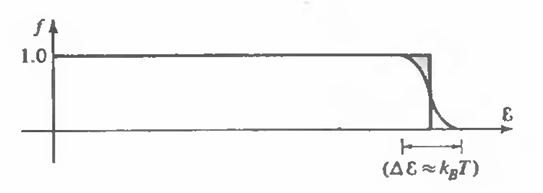
\includegraphics[width=0.6\textwidth]{images/1-Proprietà-Metalli/FDTmagg0.png}
	\caption{all'aumentare della temperatura la distribuzione di Fermi Dirac non è più una funzione a gradino}
	\label{fig:FDTmagg0}
\end{figure}

In tale grafico si nota che, all'aumentare della temperatura, la distribuzione di Fermi-Dirac non mantiene più la forma a gradino, ma si arrotonda. Le particelle che vengono "spostate" a destra (oltre il livello di Fermi) sono quelle che contribuiscono alla conduzione.\\\\
Per stimare le variazioni energetiche a temperatura finita si osserva che le particelle che cambiano stato sono quelle in un intorno di ampiezza $\sim K_B T$ intorno a $\varepsilon_f$. Se il numero di queste particelle è pari a $g(E_f) \cdot K_B T$, e ciascuna acquisisce in media un'energia dell'ordine di $K_B T$, allora la variazione di energia è:
\[
\Delta U \approx g(E_f) (K_B T)^2\,.
\]
Pertanto il calore specifico (per unità di volume) è:
\begin{equation}
	\frac{\partial \Delta U}{\partial T} \approx 2 K_B^2 T\,g(E_f)\,.
	\label{eqn:Cv_explicit}
\end{equation}
Questa correzione al calore specifico spiega il comportamento sperimentale, in cui il calore specifico diminuisce tendendo a zero quando $T\to 0$, contrariamente al caso classico in cui si avrebbe un calore specifico costante $C_V = 3R$.

\bigskip
\noindent
Analizziamo ora la dipendenza dell'energia totale $U$ (o della densità energetica $u=\frac{U}{V}$) dalla temperatura. L'energia totale del sistema è data da:
\[
U= 2 \sum_{\vec{k}} \varepsilon(\vec{k})\, f(\varepsilon(\vec{k}))\,,
\]
dove $f(\varepsilon)$ è la distribuzione di Fermi-Dirac. Passando dalla somma ad un integrale, si ha:
\[
u= \frac{U}{V}= 2\int \frac{d\vec{k}}{8\pi^3} \varepsilon(\vec{k})\, f(\varepsilon(\vec{k}))\,.
\]
Utilizzando la relazione tra lo spazio dei vettori $k$ ed il numero di stati in funzione dell'energia, si introduce la densità degli stati $g(\varepsilon)$; pertanto:
\[
u= \int_{0}^{\infty} d\varepsilon\, g(\varepsilon)\, \varepsilon\, f(\varepsilon)\,,
\]
e analogamente la densità delle particelle è:
\[
n= \int_{0}^{\infty} d\varepsilon\, g(\varepsilon)\, f(\varepsilon)\,.
\]

A temperature finite, per calcolare integrali del tipo 
\[
I= \int_{-\infty}^{\infty} H(\varepsilon) f(\varepsilon)\,d\varepsilon\,,
\]
è utile espandere $H(\varepsilon)$ in un intorno del potenziale chimico $\mu$. L'espansione (nota come espansione di Sommerfeld) è:
\[
\int_{-\infty}^{\infty} H(\varepsilon) f(\varepsilon) d\varepsilon = \int_{-\infty}^{\mu} H(\varepsilon) d\varepsilon + \frac{\pi^2}{6}(K_B T)^2\, H'(\mu) + O\left(\frac{K_B T}{\mu}\right)^4\,.
\]
Applicando questa espansione sia per $u$ che per $n$, e limitando l'integrazione da 0 a $\mu$ (poiché $g(\varepsilon)=0$ per $\varepsilon<0$), si ottengono:
\[
u= \int_0^\mu \varepsilon\, g(\varepsilon)\,d\varepsilon + \frac{\pi^2}{6}(K_B T)^2 \left[\varepsilon\,g'(\mu)+ g(\mu)\right] + O(T^4)
\]
e
\[
n= \int_0^\mu g(\varepsilon)\,d\varepsilon + \frac{\pi^2}{6}(K_B T)^2\, g'(\mu) + O(T^4)\,.
\]
Il potenziale chimico cambia con la temperatura e non coincide perfettamente con l'energia di Fermi, per cui si attua una seconda espansione:
\[ \int_0^\mu H(\varepsilon) d\varepsilon = \int_0^{\varepsilon_f} H(\varepsilon)d(\varepsilon) + (\mu - \varepsilon_f) H(\varepsilon_f) \]
Quindi ottengo:
\[ u = \int_0^{\varepsilon_f} \varepsilon\cdot  g(\varepsilon)\dot d\varepsilon  + (\mu - \varepsilon_f) g(\varepsilon_f)\cdot \varepsilon_f  + \frac{\pi^2}{6}(K_b T)^2 \bigl[g'(\varepsilon_f)  + g(\varepsilon_f)\bigr]+ O(T^4) \]
\[ n = \int_0^{\varepsilon_f} g(\varepsilon)\cdot d\varepsilon +\left\{(\mu - \varepsilon_f) g(\varepsilon_f) + \frac{\pi^2}{6}(K_b T)^2 g'(\varepsilon_f) \right\} \]
siccome $\int_0^\mu g(\varepsilon)d\varepsilon = n$ per definizione, questo significa che  \\
\[\left\{(\mu - \varepsilon_f) g(\varepsilon_f) + \frac{\pi^2}{6}(K_b T)^2 g'(\varepsilon_f) \right\} = 0\]
altrimenti non sto conservano il numero totale di particelle nel caso degli elettroni, da questa relazione possiamo quindi ricavare il poetnziale chimico:
\begin{equation}
	\mu = \varepsilon_f - \frac{\pi^2}{6} (K_b T)^2 \cdot \frac{g'(\varepsilon_f) }{g(\varepsilon_f) }
	\label{eqn:muT}
\end{equation}
Il segno del termine correttivo dipende dal segno di $g'(\varepsilon_f)$ e ciò spiega il piccolo spostamento di $\mu$ con la temperatura, come illustrato ad esempio in Figura \ref{fig:fermidirac2}.
\begin{figure} [H]
	\centering
	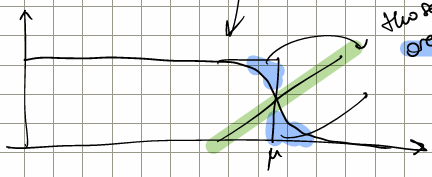
\includegraphics[width=0.4\textwidth]{images/1-Proprietà-Metalli/fermidirac2.png}
	\caption{}
	\label{fig:fermidirac2}
\end{figure}

\bigskip
\subsection{Densità di stati}

Quanti stati hanno energia compresa tra $\varepsilon$ e $\varepsilon + d\varepsilon$? In generale la densità di stati è definita da:
\begin{equation}
	g(\varepsilon)= \int \frac{d\vec{k}}{4\pi^3} \, \delta(\varepsilon-\varepsilon(\vec{k}))\,.
	\label{eqn:dos_def}
\end{equation}
Per valutare questo integrale, anziché lavorare direttamente con la delta di Dirac, si conta il numero di stati in una corona sferica nel $k$-space. La relazione tra una variazione infinitesima di energia $d\varepsilon$ e quella di $k$ è data da:
\[
\varepsilon + d\varepsilon \approx \varepsilon + |\vec{\nabla} \varepsilon(k)|\, \delta k(k) \quad \Longrightarrow \quad \delta k(k)= \frac{d\varepsilon}{|\vec{\nabla} \varepsilon(k)|}\,.
\]
\begin{figure} [H]
	\centering
	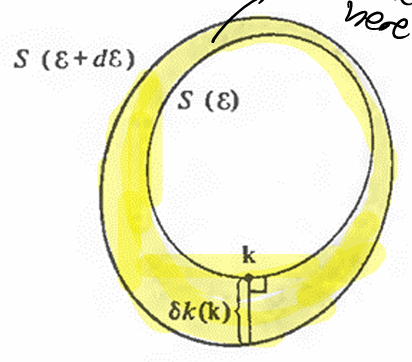
\includegraphics[width=0.4\textwidth]{images/1-Proprietà-Metalli/coronacircolare.png}
	\caption{}
	\label{fig:corona-circolare}
\end{figure}

Pertanto, il numero di stati con energia compresa in $[\varepsilon,\varepsilon+d\varepsilon]$ è:
\[
g(\varepsilon) \, d\varepsilon = \int_{S(\varepsilon)} \frac{dS}{4\pi^3}\,\frac{d\varepsilon}{|\vec{\nabla} \varepsilon(k)|}\,,
\]
da cui
\[
g(\varepsilon)= \int_{S(\varepsilon)} \frac{dS}{4\pi^3}\,\frac{1}{|\vec{\nabla} \varepsilon(k)|}\,.
\]
 In 3D $g(\varepsilon)$ è integrabile ma ci sono delle divergenze di $\frac{dg}{d\varepsilon}$ chiamate \textbf{singolarità di van Hove}, e sono mostrate in Figura \ref{fig:densstati3D}\\\\
\begin{figure} [H]
	\centering
	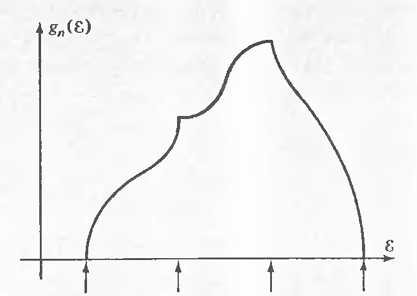
\includegraphics[width=0.4\textwidth]{images/1-Proprietà-Metalli/densstati3d.png}
	\caption{in figura i punti critici vengono indicati dalle frecce}
	\label{fig:densstati3D}
\end{figure}

Nel caso in cui
\[
\varepsilon(k)= \frac{\hbar^2 k^2}{2m}\,,
\]
si ha, in 1D, la derivata:
\[
\frac{d\varepsilon}{dk}= \frac{\hbar^2 k}{m}\,,
\]
e passando all'integrazione in $k$-space in 3D, contando il numero di stati in una corona sferica (tenendo conto della degenerazione di spin), il numero di stati tra $k$ e $k+dk$ è dato da:
\[
g(\varepsilon)d\varepsilon= 2\cdot \frac{1}{8\pi^3}\cdot 4\pi k^2\, dk\,.
\]
Poiché
\[
\frac{d\varepsilon}{dk}= \frac{\hbar^2 k}{m} \quad \Longrightarrow \quad dk= \frac{m}{\hbar^2 k}\,d\varepsilon\,,
\]
si ottiene:
\[
g(\varepsilon)= \frac{1}{\pi^2}\, k^2 \cdot \frac{m}{\hbar^2 k}= \frac{m}{\pi^2 \hbar^2}\, k\,.
\]
Infine, esprimendo $k$ in funzione dell'energia:
\[
k= \sqrt{\frac{2m\varepsilon}{\hbar^2}}\quad \implies \quad g(\varepsilon)= \frac{m}{\pi^2 \hbar^2}\sqrt{\frac{2m\varepsilon}{\hbar^2}} \propto \sqrt{\varepsilon}\,.
\]
Questo risultato corrisponde al noto andamento di $g(\varepsilon)$ nei metalli. In figura (vedi Figura \ref{fig:dosvsen}) si mostra l'andamento della densità degli stati moltiplicata per la distribuzione di Fermi-Dirac.
\begin{figure} [H]
	\centering
	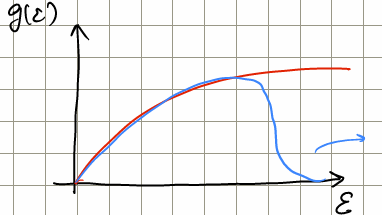
\includegraphics[width=0.4\textwidth]{images/1-Proprietà-Metalli/dosvsen.png}
	\caption{l'occupazione degli stati è indicata dalla curva in azzurro ed è così perchè è moltiplicata per la distribuzione di Fermi dirac}
	\label{fig:dosvsen}
\end{figure}

\subsection{Calcolo dell'energia totale e del calore specifico}
La densità di energia totale invece è data da:
\begin{equation}
\begin{split}
     u &= \int_0^{\varepsilon_f} \varepsilon\cdot  g(\varepsilon)\dot d\varepsilon  + \cancel{(\mu - \varepsilon_f) g(\varepsilon_f)\cdot \varepsilon_f}  + \cancel{\frac{\pi^2}{6}(K_b T)^2 \bigl[g'(\varepsilon_f)}  + g(\varepsilon_f)\bigr] \\
     &= \int_0^{\varepsilon_f} \varepsilon \ g(\varepsilon_f) d\varepsilon + \frac{\pi^2}{6} (KT)^2g(\varepsilon_f) = u_0 +  \frac{\pi^2}{6} (KT)^2g(\varepsilon_f)
\end{split}
\end{equation}
dove $\int_0^{\varepsilon_f} \varepsilon \ g(\varepsilon_f) d\varepsilon = u_0(T=0)$. \\\\
Da cui ottengo:
\begin{equation}
    C_v =\frac{du}{dt}\biggr|_v =\frac{\pi^2}{3}\cdot K_b^2T\cdot g(\varepsilon_f)
    \label{eqn:uconu0}
\end{equation}
Questo risultato, in accordo con le misurazioni sperimentali, mostra che il contributo degli elettroni al calore specifico è proporzionale a $T$ per $T\to 0$, mentre il contributo classico (basato sui soli gradi di libertà armonici) darebbe un valore costante.

\bigskip
\noindent
Si nota infine che, in un metallo, solo una piccola frazione degli elettroni (quelli prossimi a $\varepsilon_f$, il cosiddetto "strato di superficie" della sfera di Fermi, dell'ordine di $\sim K_B T$) è in grado di partecipare al trasporto termico e alla conduzione elettrica; il resto degli elettroni resta vincolato negli stati profondi e non contribuisce alle proprietà termiche a basse temperature.

\bigskip
\subsection{Calcolo esplicito della densità degli stati all'energia di Fermi}
Calcoliamo la densità di stati all'energia di Fermi. L'energia di Fermi in funzione di n è data da: $\varepsilon_f = \frac{\hbar^2}{2m}(3\pi^2 n)^{\frac{2}{3}}$ quindi:
\[ g(\varepsilon_f) = \frac{m}{\hbar^2 \pi^2} \sqrt{\frac{2m}{\hbar^2}} \sqrt{\varepsilon_f} \]
moltiplico e divido per $\frac{3}{2}\cdot n$ e ottengo:
\[ g(\varepsilon_f) =  \frac{3n}{2} \frac{2}{3n} \frac{m}{\hbar^2 \pi^2} \sqrt{\frac{2m}{\hbar^2}} \sqrt{\varepsilon_f} =  \frac{3n}{2} \left[ \left( \frac{1}{3\pi^2 n} \right) \left( \frac{2m}{\hbar^2} \right)^{\frac{3}{2}} \sqrt{\varepsilon_f} \right] = \frac{3n}{2} \frac{{\varepsilon_f}^\frac{1}{2}}{\varepsilon_f^{\frac{3}{2}}} = \frac{3}{2} \frac{n}{\varepsilon_f} \]
\[ \implies \mu =  \varepsilon_f - \frac{\pi^2}{6} (K_b T)^2 \frac{g'(\varepsilon_f) }{g(\varepsilon_f) }= [g(\varepsilon) \propto \sqrt{\varepsilon}] = \varepsilon_f \left[ 1 - \frac{1}{3} \left( \frac{\pi K_b T}{2 \varepsilon_f} \right)^2 \right] \]
considerando il calore specifico nella \ref{eqn:uconu0} nel caso dei metalli alcalini si ottiene:
\[ C_v = \left( \frac{\partial u}{\partial T} \right)_n = \frac{\pi^2}{3} K_b^2 T \ g(\varepsilon_f) = \frac{\pi^2}{2}\frac{n}{\varepsilon_f}K_b^2\cdot T\]
Confrontando con il risultato classico, che darebbe (utilizzando il modello di Einstein per i fononi, ad esempio):
\[
u= \frac{9}{2}\, K_B\, T\, n \quad \Longrightarrow \quad C_v^{\text{classico}}= \frac{9}{2}\,K_B\, n\,,
\]
si evidenzia come, a temperatura ambiente, solo una piccolissima frazione degli elettroni (quelli in prossimità di $\varepsilon_f$) contribuisce al calore specifico, mentre la maggior parte degli elettroni (al di sotto dell'energia di Fermi) rimane "congelata" e non partecipa all'aumento di energia termica.

\bigskip
\noindent
In Figura \ref{fig:cvCLvsQ} viene mostrato un confronto tra il calore specifico classico (costante, in nero) e quello corretto (che cresce linearmente con $T$, in viola), in cui la linea tratteggiata indica la temperatura ambiente.

\begin{figure}[H]
	\centering
	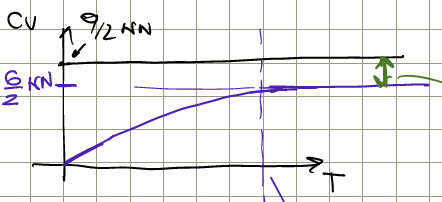
\includegraphics[width=0.5\textwidth]{images/1-Proprietà-Metalli/cvCLvsQ.png}
	\caption{Confronto tra il comportamento classico (costante) del calore specifico e il comportamento corretto (lineare in $T$) per i metalli.}
	\label{fig:cvCLvsQ}
\end{figure}

\bigskip
\noindent
Infine, si osserva che il numero di elettroni che "saltano" (cioè, che modificano il loro stato energetico a causa dell'aumento termico) è estremamente piccolo rispetto al numero totale, come illustrato in Figura \ref{fig:FD3}.

\begin{figure}[H]
	\centering
	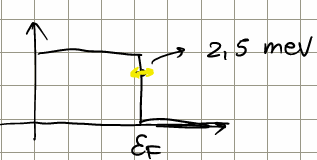
\includegraphics[width=0.5\textwidth]{images/1-Proprietà-Metalli/FD3.png}
	\caption{Distribuzione di Fermi-Dirac che evidenzia la piccola frazione di elettroni attivi (vicino a $\varepsilon_f$) a temperatura ambiente.}
	\label{fig:FD3}
\end{figure}
\chapter{Cristalli}
\label{ch:cristalli}
I solidi vengono descritti da strutture ordinate dette strutture cristalline: La prima volta che si ebbe l'intuizione che c'è dell'ordine nella struttura della materia fu grazie alla diffrazione dei Raggi X. Se un raggio X che trapassa un materiale alla sua uscita presenza di un reticolo di diffrazione implica che c'è una struttura ben precisa al suo interno. 
\begin{figure} [H]
	\centering
	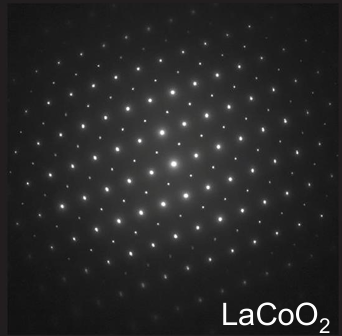
\includegraphics[width=0.15\textwidth]{images/2-Cristalli/xraydiff.png}
	\caption{qui si osserva il reticolo di diffrazione del \ce{LaCO2} da cui si deduce che in realtà la struttura è più complicata poiché ho dei punti più luminosi di altri}
	\label{fig:xraydiff}
\end{figure}

In natura gli elementi si presentano in diverse strutture e ce ne possono essere di diversi tipi: 
\begin{figure} [H]
	\centering
	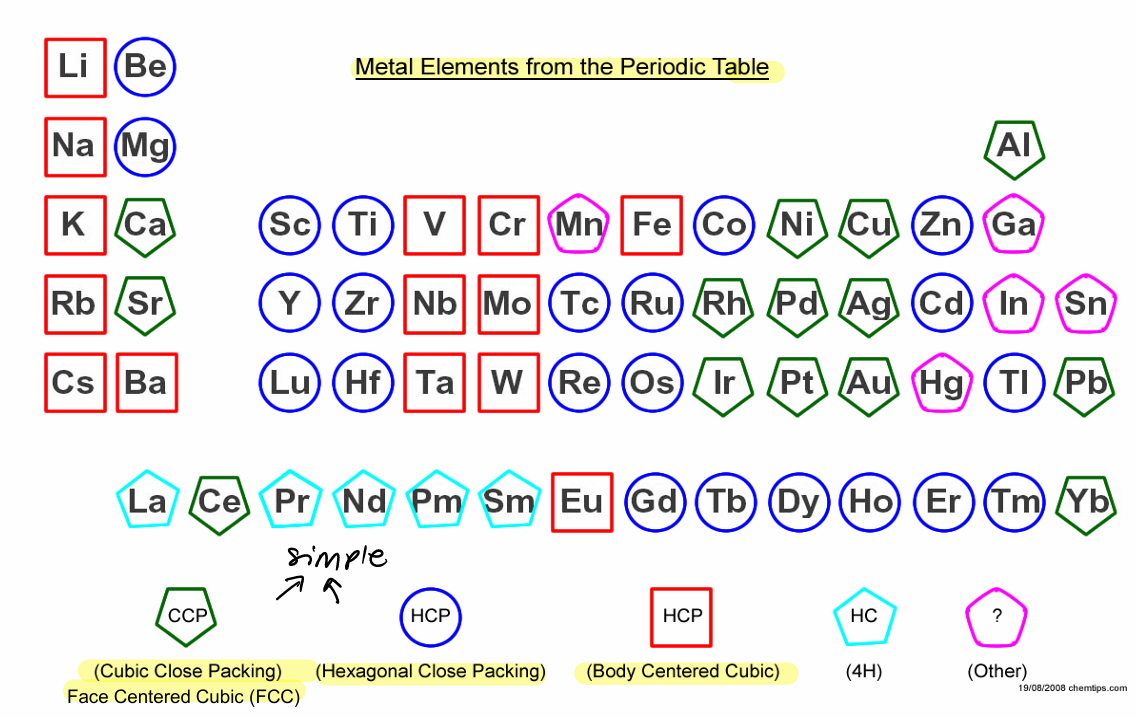
\includegraphics[width=0.55\textwidth]{images/2-Cristalli/strutturacrist.png}
	\caption{}
	\label{fig:strutturacrist}
\end{figure} 

\section{Reticolo di Bravais}
Un concetto fondamentale nella descrizione di qualsiasi tipo di solido cristallino è quello del \textbf{reticolo di Bravais}. Ci sono 2 possibili definizioni equivalenti per il reticolo di Bravais e sono:
\begin{itemize}
	\item Un reticolo di Bravais è un array infinito di punti discreti con posizioni e orientazioni precise che sono esattamente le stesse a prescindere dal punto in cui l'array viene osservato.
	\item Un reticolo di Bravais (tridimensionale) consiste in tutti i punti che possono descritti con vettore di posizione R della forma: \begin{equation} \vec{R} = n_1 \vec{a}_1 + n_2\vec{a}_2 + n_3 \vec{a}_3 \end{equation} dove $a_1,a_2,a_3$ sono 3 vettori qualsiasi che non appartengono allo stesso piano (non complanari) ed $n_1,n_2,n_3$ sono degli interi. Il punto $\sum_i n_i a_i$ si raggiunge facendo $n_i$ passi di lunghezza $a_i$ nella direzione i. 
\end{itemize}
Se sommo due elementi del reticolo di Bravais ottengo ancora un elemento del reticolo di Bravais: $R \in BL, \ R' \in BL \implies R + R' \in BL, \ R-R' \in BL$ \\
\begin{figure} [H]
	\centering
	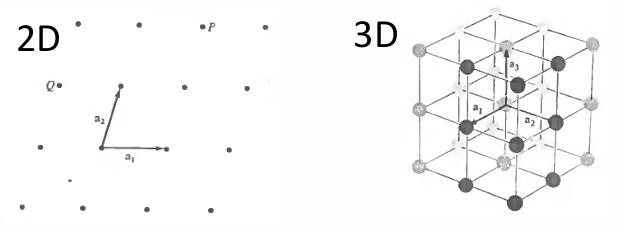
\includegraphics[width=0.55\textwidth]{images/2-Cristalli/reticoliB.png}
	\caption{Questi sono esempi di reticoli di Bravais: nel caso 2D avendo $a_1$ e $a_2$ e nel caso 3D avendo $a_1, a_2$ e $a_3$ posso ricostruire l'intero cristallo}
	\label{fig:reticoliB}
\end{figure} 

Un'altra definizione equivalente di reticolo di Bravais è: un set discreto di vettori (non appartenenti allo stesso piano) invarianti per somma e sottrazione.
\begin{figure} [H]
	\centering
	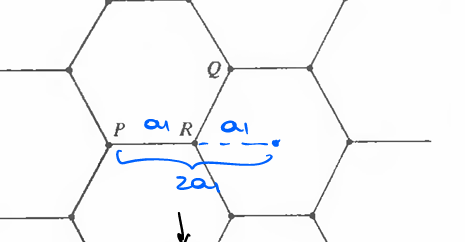
\includegraphics[width=0.55\textwidth]{images/2-Cristalli/nonBL.png}
	\caption{In figura è riportato un esempio del reticolo cristallino del Grafene che NON è un reticolo di Bravais, questo perché se al segmeto PR sommo a, che dovrebbe essere il passo del reticolo raggiungo una zona in cui non è presente nessun punto (nessun atomo), se fosse un reticolo di Bravais con $2a$ dovrei raggiungere un punto del reticolo di Bravais perché dovrei riuscire a ricostruire tutto il reticolo cristallino}
	\label{fig:nonBL}
\end{figure}

Ho una scelta infinita di vettori $a$, che vengono denominati \textbf{vettori primitivi} per definire un reticolo di Bravais, ma alcuni sono meglio di altri, vedremo le diverse scelte per diversi tipi di reticoli di Bravais.

\subsection{Cubo Semplice}
\begin{figure} [H]
	\centering
	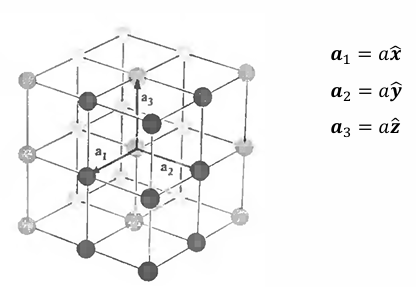
\includegraphics[width=0.55\textwidth]{images/2-Cristalli/cubosemplice.png}
	\caption{i vettori primitivi sono 3 vettori perpendicolari}
	\label{fig:cubosemplice}
\end{figure} 

\subsection{Body Centered Cube (BCC)}
\begin{figure} [H]
	\centering
	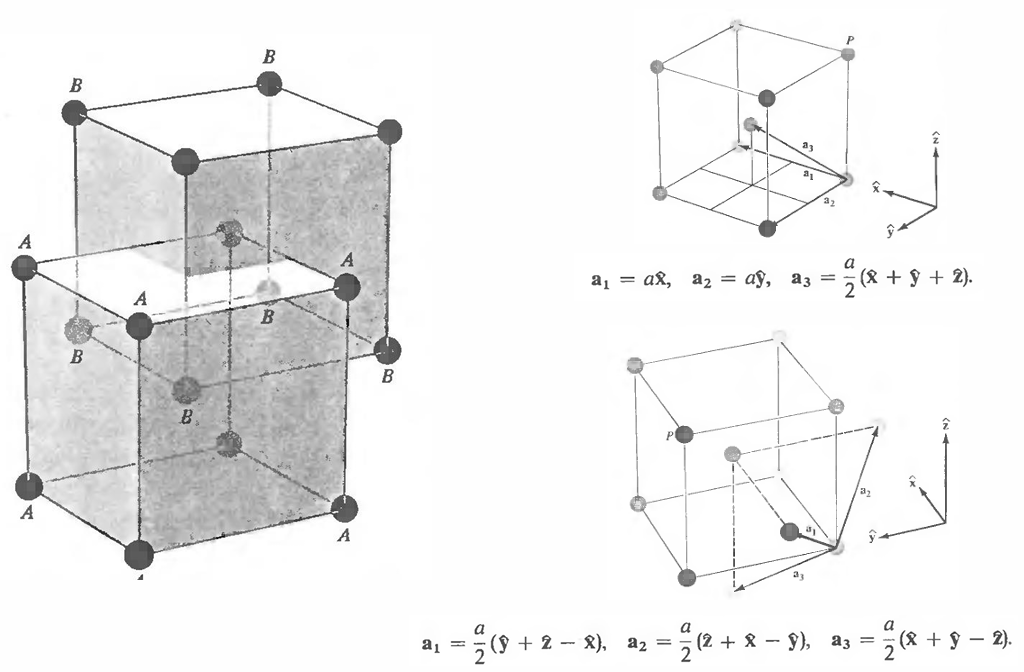
\includegraphics[width=0.9\textwidth]{images/2-Cristalli/BCC.png}
	\caption{}
	\label{fig:BCC}
\end{figure} 
Il cubo a corpo centrato è formato da due reticoli cubici compenetranti, in pratica è un cubo con un atomo al centro, dalla Figura \ref{fig:dimBCC} si dimostra che il BCC è un reticolo di Bravais. 
\begin{figure} [H]
	\centering
	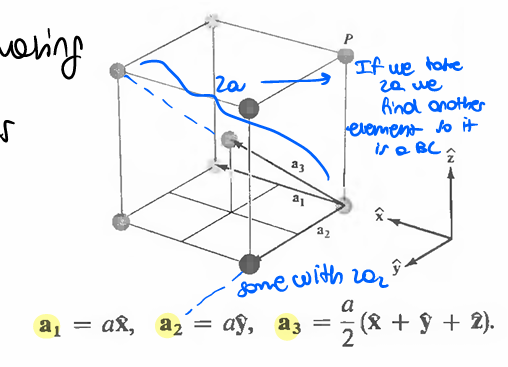
\includegraphics[width=0.5\textwidth]{images/2-Cristalli/dimBCC.png}
	\caption{Prendendo due volte il vettore $a_3$ incontro un atomo del cristallo quindi è per questo che è un reticolo di Bravais}
	\label{fig:dimBCC}
\end{figure} 
I metalli che presentano una struttura a BCC sono i metalli più duri, la presenza di quell'atomo centrale nel cubo crea frizione, i metalli deformabili invece sono formati da strati impilati l'uno sopra l'altro quindi molto più facili da deformare o spezzare (elementi di questo tipo sono Ba, Cr, Cs, Fe, K).

\subsection{Face Centered Cube (FCC)}
In questo caso invece ho un atomo al centro delle facce di ogni cubo. La struttura è piramidale con strati successivi orientati in maniera alternata.
\begin{figure}[H]
	\centering
	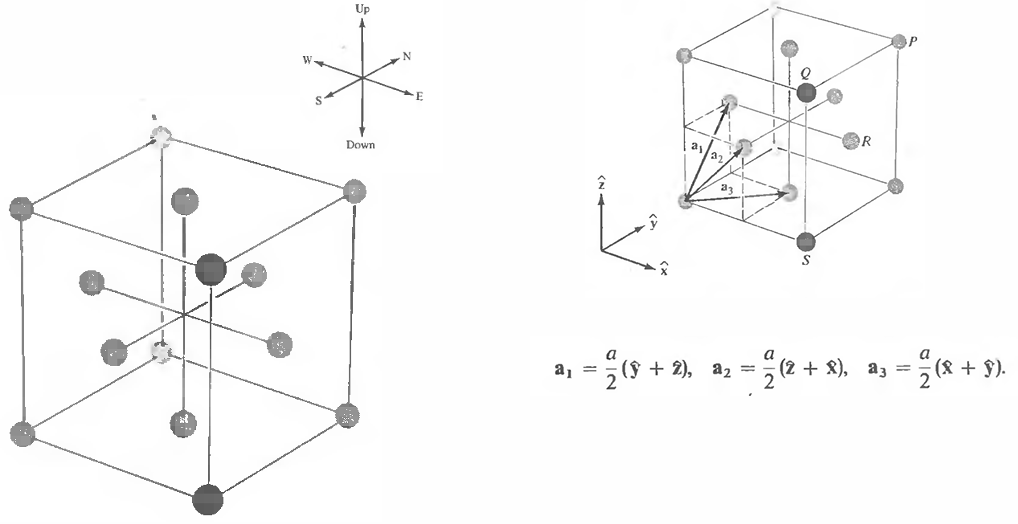
\includegraphics[width=0.9\textwidth]{images/2-Cristalli/FCC.png}
	\caption{}
	\label{fig:FCC}
\end{figure} 
Sono gli elementi più facili da deformare (gli elementi di questo tipo sono: Ar, Ag, Al, Au, Ca, Ce, $\beta$-Co, Cu).



\subsubsection{Coordination Number}
Il \textbf{coordination number} è il numero di primi vicini che ogni atomo ha all'interno di un certo cristallo, per esempio per il cubo semplice sono 6 per il BCC 8 e per l'FCC 12.

\subsection{Cella Primitiva Unitaria}
Una \textbf{cella primitiva unitaria} è una porzione di spazio (un volume) che se traslata lungo i vettori del reticolo di Bravais riempie tutto lo spazio senza lasciare buchi o sovrapponendosi a qualcosa. Anche in questo caso ci sono più scelte possibili di cella primitiva ma ce ne sono alcune che sono più importanti di altre. Le diverse scelte di cella primitiva però dovranno avere lo stesso volume. 
\\~\\
Una cella primitiva molto importante è la \textbf{cella di Wigner Seitz} che è una cella primitiva che mantiene la simmetria locale del cristallo. La WSC di un punto del reticolo è data dalla regione di spazio più vicina a quel punto rispetto a qualsiasi altro punto del reticolo. In Figura \ref{fig:WSC} è mostrato un esempio di una cella WSC.
\begin{figure} [H]
	\centering
	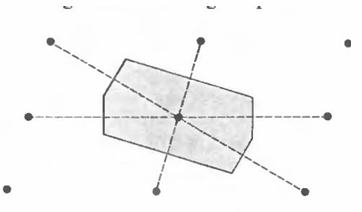
\includegraphics[width=0.5\textwidth]{images/2-Cristalli/WSC.png}
	\caption{Per costruire una cella di Wigner Seitz taglio a metà le linee che connettono tutti i gli altri atomi all'atomo centrale}
	\label{fig:WSC}
\end{figure} 

La WSC del BCC è un ottaedro troncato e quella dell'FCC è un dodecaedro rombico, la simmetria della WSC è correlata a quella del reticolo perché infatti nel caso del BCC dove abbiamo come numero di coordinazione 8 (quindi 8 primi vicini) abbiamo un ottaedro mentre nel caso dell'FCC che ha come numero di coordinazione 12 abbiamo un dodecaedro.

\section{Struttura cristallina, reticoli con base}
Una struttura cristallina non è un reticolo di Bravais e consiste in copie identiche della stessa unità fisica, chiamata \textbf{base}, localizzata nei punti di un reticolo di Bravais. \\
Un atomo è al centro del reticolo di Bravais e descrivo l'altro rispetto al reticolo quindi la sua posizione sarà $\Vec{R}+d$. In pratica colleziono coppie di atomi e questi due possono essere descritti da un reticolo di Bravais. La posizione dell'atomo è descritta da:
\begin{itemize}
	\item dal centro della cella unitaria descritta da un reticolo di Bravais $\implies \Vec{R}$
	\item dalla posizione relativa degli atomi all'interno della cella unitaria $\implies \Vec{R} + \Vec{d}$
\end{itemize}
\begin{figure} [H]
	\centering
	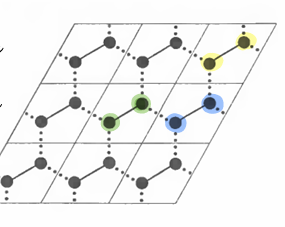
\includegraphics[width=0.5\textwidth]{images/2-Cristalli/struttcristall.png}
	\caption{}
	\label{fig:struttcristall}
\end{figure} 
\subsection{Strutture a diamante}
Nelle figure \ref{fig:diamantebase1} e \ref{fig:diamantebase2} è riportata una tipologia di cristalli con base che sono i cristalli con \textbf{struttura a diamante} che sono degli FCC con base, inoltre i siti atomici hanno tutti una struttura tetraedrica ad ibridizzazione $sp^3$ con numero di primi vicini 4.
\begin{figure} [H]
	\centering
	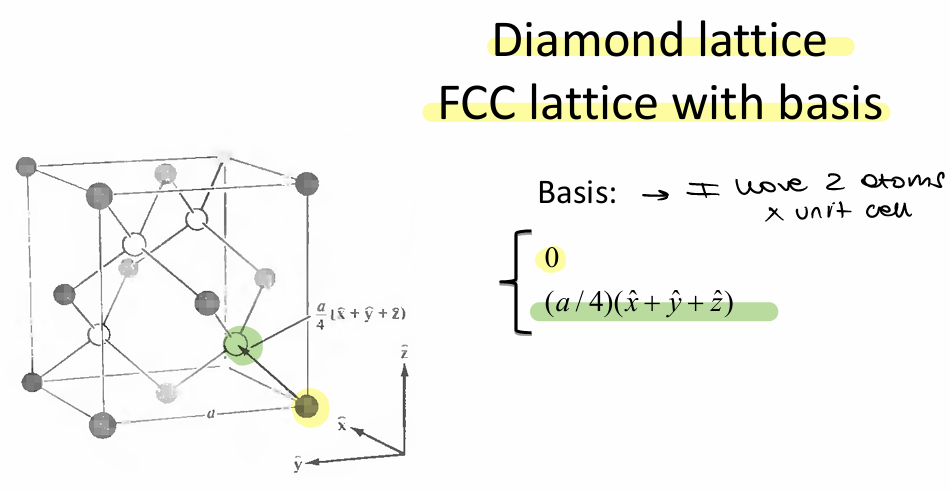
\includegraphics[width=0.9\textwidth]{images/2-Cristalli/diamantebase1.png}
	\caption{}
	\label{fig:diamantebase1}
\end{figure} 
\begin{figure} [H]
	\centering
	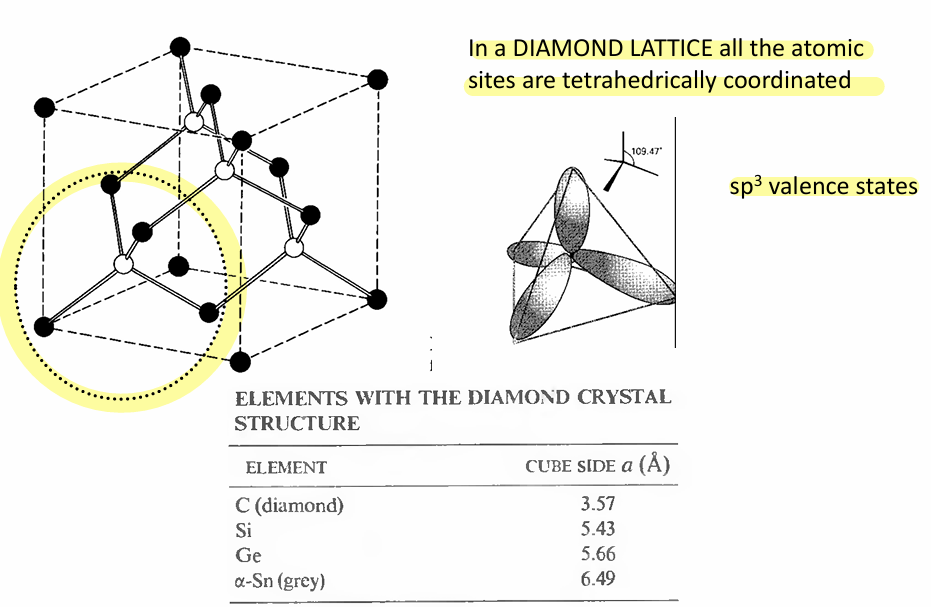
\includegraphics[width=0.9\textwidth]{images/2-Cristalli/diamantebase2.png}
	\caption{}
	\label{fig:diamantebase2}
\end{figure} 

Un altro esempio di cristallo con base che è un diamante FCC è la \textbf{zincoblenda}, in questo caso però si hanno due atomi all'interno della cella che sono diversi (esempi di cristalli sono: ZnS, CuF, CuCl ecc). Tieni a mente che non sono dei reticoli di Bravais

\subsection{Hexagonal Closed Packed Structure (HCP)}
Anche se non è un reticolo di Bravais l'HCP è una delle strutture più presenti in natura assieme ai reticoli di Bravais FCC e BCC. La struttura consiste in due reticoli di Bravais ad esagono semplice inter-penetranti spostati l'uno dall'altro di $\frac{a_1}{3}+\frac{a_2}{3}+\frac{a_3}{2}$. 
\begin{figure} [H]
	\centering
	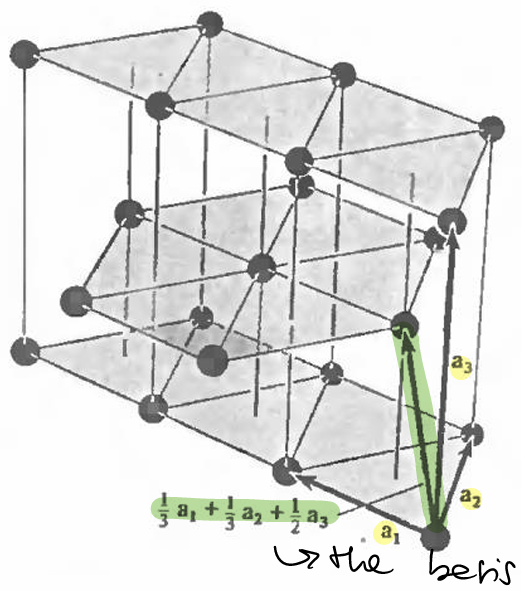
\includegraphics[width=0.35\textwidth]{images/2-Cristalli/HCP1.png}
	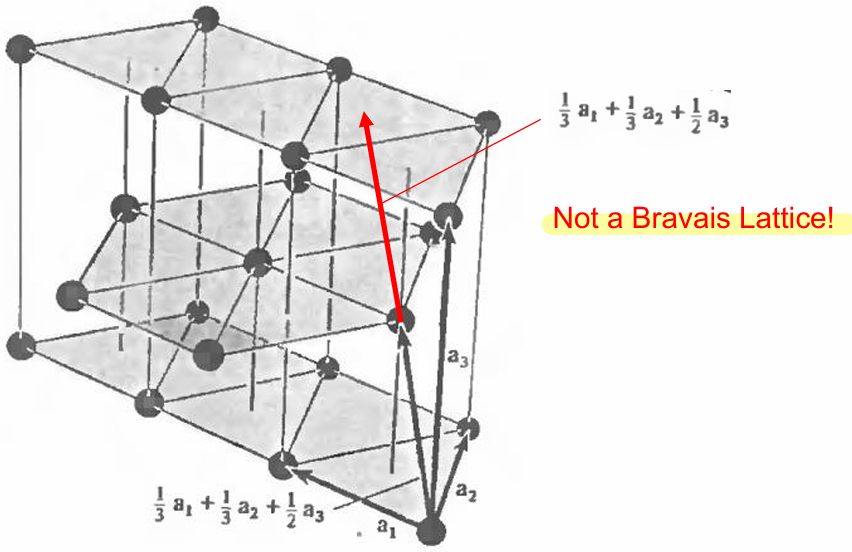
\includegraphics[width=0.55\textwidth]{images/2-Cristalli/HCP2.png}
	\caption{si può notare che l'HCP non è un reticolo di Bravais}
	\label{fig:HCP}
\end{figure} 

Si può notare che è un tipo di struttura che promuove atomi con forze isotropiche e a corto raggio (Forza di Coulumb o di Wan Der Waals), mentre atomi in cui prevale la direzionalità e forze a lungo raggio favoriscono la formazione di strutture FCC piuttosto che HCP.\\ 

\subsection{Altri reticoli con base}
\subsubsection{Struttura del cloruro di sodio}
È formato da 2 diversi atomi quindi rompo la simmetria perciò sicuramente non può essere descritto da un semplice reticolo di Bravais ma è un reticolo di Bravais FCC (quindi ha i vettori primitivi dell'FCC, e lo forma con cloro e ha il sodio all'interno della cella unitaria) con base $\frac{a}{2}(\hat{x}+\hat{y} + \hat{z})$. È un cristallo ionico, degli esempi cristalli di questa forma oltre all'NaCl sono NaF, NaI, KBr ecc...
\begin{figure} [H]
	\centering
	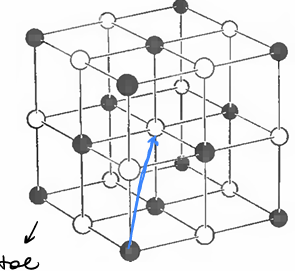
\includegraphics[width=0.35\textwidth]{images/2-Cristalli/NaCl.png}
	\caption{struttura cristallina dell'NaCl}
	\label{fig:NaCl}
\end{figure}

\subsubsection{Struttura del cloruro di cesio}
È un BCC con base $\frac{a}{2}(\hat{x}+\hat{y} + \hat{z})$ . Le forze principali in gioco sono le forze di coulomb e questa è la struttura che minimizza l'energia. Esempi di cristalli con questa struttura oltre al CsCl sono: CsBr e CsI
\begin{figure} [H]
	\centering
	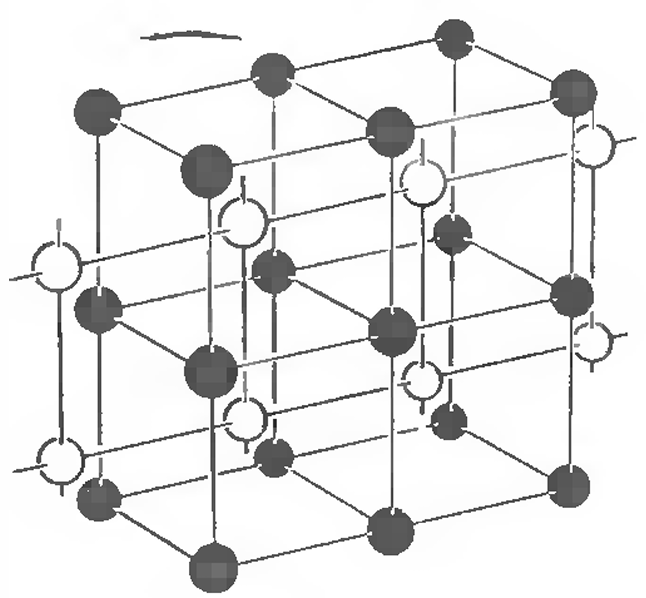
\includegraphics[width=0.35\textwidth]{images/2-Cristalli/CsCl.png}
	\caption{struttura cristallina dell'CsCl, l'atomo bianco al centro del BCC è un atomo diverso dagli altri quindi è per questo che necessito un reticolo di Bravais con base}
	\label{fig:CsCl}
\end{figure}
In poche parole se ho due atomi diversi nel cristallo sicuramente non sarà descritto da un reticolo di Bravais.


\section{Reticolo Reciproco}

Quando si eseguono esperimenti di diffrazione con raggi X per studiare la struttura cristallina, ciò che viene effettivamente osservato è la trasformata di Fourier delle posizioni degli atomi. In questo contesto, la trasformata di Fourier di un reticolo di Bravais risulta essere essa stessa un reticolo di Bravais, detto \textbf{reticolo di Bravais reciproco}.

\subsection*{Definizione di Reticolo Reciproco}

La definizione corretta è la seguente: l'insieme dei vettori d'onda \(\vec{K}\) tali che le onde piane associate \(e^{i\vec{K}\cdot \vec{r}}\) abbiano la stessa periodicità del dato reticolo di Bravais, costituisce il reticolo reciproco. In altre parole, per ogni vettore di traslazione \(\vec{R}\) del reticolo (cioè \(\vec{R}\) appartenente al reticolo di Bravais) deve valere:
\[
e^{i\vec{K}\cdot (\vec{r} + \vec{R})} = e^{i\vec{K}\cdot \vec{r}} \quad \forall\, \vec{r}.
\]
Da ciò segue che:
\[
e^{i\vec{K}\cdot \vec{R}} = 1.
\]
Pertanto, l'insieme dei vettori \(\vec{K}\) che soddisfano la condizione
\[
e^{i\vec{K}\cdot \vec{R}} = 1 \quad \text{per ogni } \vec{R} \text{ del reticolo di Bravais}
\]
definisce il reticolo reciproco.

Notiamo che se \(e^{i\vec{K}\cdot \vec{R}} = 1\) per ogni \(\vec{R}\), l'onda piana \(e^{i\vec{K}\cdot \vec{r}}\) assume lo stesso valore in tutti i punti del reticolo, cioè la funzione è periodica con la medesima periodicità del reticolo reale. In sostanza, il reticolo reciproco è costituito dai vettori \(\vec{K}\) associati ad onde piane la cui periodicità coincide con quella del reticolo di Bravais.

\subsection*{Chiusura per Addizione e Sottrazione}

Una proprietà importante del reticolo reciproco è la sua invarianza rispetto ad addizione e sottrazione. Infatti, se \( \vec{K},\, \vec{K'} \) appartengono al reticolo reciproco, allora:
\[
e^{i(\vec{K}+\vec{K'}) \cdot \vec{R}} = e^{i\vec{K}\cdot \vec{R}}\, e^{i\vec{K'}\cdot \vec{R}} = 1 \cdot 1 = 1,
\]
quindi anche \( \vec{K}+\vec{K'} \) appartiene al reticolo reciproco. Lo stesso vale per la sottrazione. Questo fatto mostra che il reticolo reciproco possiede la struttura di un reticolo di Bravais.

\subsection*{Relazione tra Reticolo di Bravais e Reticolo Reciproco}

Il reticolo reciproco permette di determinare geometricamente il reticolo di Bravais originale. Se sono dati i vettori primitivi \( \vec{a}_1, \vec{a}_2, \vec{a}_3 \) del reticolo di Bravais, i vettori primitivi del reticolo reciproco si definiscono in questo modo:
\[
\vec{b}_1 = 2\pi\, \frac{\vec{a}_2 \times \vec{a}_3}{\vec{a}_1 \cdot (\vec{a}_2 \times \vec{a}_3)},
\]
\[
\vec{b}_2 = 2\pi\, \frac{\vec{a}_3 \times \vec{a}_1}{\vec{a}_1 \cdot (\vec{a}_2 \times \vec{a}_3)},
\]
\[
\vec{b}_3 = 2\pi\, \frac{\vec{a}_1 \times \vec{a}_2}{\vec{a}_1 \cdot (\vec{a}_2 \times \vec{a}_3)}.
\]
Da queste definizioni si può dimostrare che i vettori primitivi \(\vec{b}_i\) soddisfano la relazione:
\[
\vec{b}_i \cdot \vec{a}_j = 2\pi\, \delta_{ij},
\]
dove \(\delta_{ij}\) è il delta di Kronecker.

\subsection*{Verifica della Condizione di Periodicità}

Per vedere che i vettori \(\vec{b}_i\) appartengono al reticolo reciproco, consideriamo un generico vettore di traslazione del reticolo reale:
\[
\vec{R} = n_1 \vec{a}_1 + n_2 \vec{a}_2 + n_3 \vec{a}_3 \quad \text{con } n_i \in \mathbb{Z}.
\]
Un generico vettore \(\vec{K}\) del reticolo reciproco si può scrivere come:
\[
\vec{K} = k_1 \vec{b}_1 + k_2 \vec{b}_2 + k_3 \vec{b}_3 \quad \text{con } k_i \in \mathbb{Z}.
\]
Il prodotto scalare risulta dunque:
\[
\vec{K} \cdot \vec{R} = k_1 n_1\, (\vec{b}_1 \cdot \vec{a}_1) + k_2 n_2\, (\vec{b}_2 \cdot \vec{a}_2) + k_3 n_3\, (\vec{b}_3 \cdot \vec{a}_3) = 2\pi (k_1 n_1 + k_2 n_2 + k_3 n_3).
\]
Pertanto:
\[
e^{i \vec{K}\cdot \vec{R}} = e^{i 2\pi (k_1 n_1 + k_2 n_2 + k_3 n_3)} = 1,
\]
il che dimostra che \(\vec{K}\) soddisfa la condizione di periodicità richiesta per appartenere al reticolo reciproco.

\subsection*{Correlazione tra Tipologie di Reticolo}

Un aspetto interessante è la relazione tra alcuni reticoli di Bravais e i loro reticoli reciproci. Ad esempio, si ha:
\begin{center}
	\begin{tabular}{|c|c|}
	\hline
	Reticolo di Bravais & Reticolo Reciproco \\ 
	\hline
	Simple Cubic (SC) & Simple Cubic (SC) \\
	\hline
	Face-Centered Cubic (FCC) & Body-Centered Cubic (BCC) \\
	\hline
	Body-Centered Cubic (BCC) & Face-Centered Cubic (FCC) \\
	\hline
	\end{tabular}
\end{center}
In altre parole, un cristallo con struttura FCC ha come reticolo reciproco una struttura BCC, e viceversa.


\section{Zona di Brillouin}
La \textbf{zona di Brillouin} è la cella di wigner seitz del reticolo reciproco. 
\\~\\
La \textbf{prima zona di Brillouin} è l'insieme di punti nello spazio reciproco/ k-space che possono essere raggiunti dall'origine senza attraversare nessun piano di Bragg.\\\\
La \textbf{seconda zona di Brillouin} è l'insieme di punti nello spazio reciproco che possono essere raggiunti dall'origine attraversando un solo piano di Bragg. \\\\
La $(n+1)$\textbf{-esima zona di Brilluoin} è l'insieme di punti nello spazio reciproco, che non stanno nella $(n-1)$-esima zona, che può essere raggiunto dalla n-esima zona di Brilluoin attraversando un solo piano di Bragg. \\
I \textbf{piani di Bragg} sono i piani che tagliano in due la connessione tra gli atomi.
\begin{figure} [H]
	\centering
	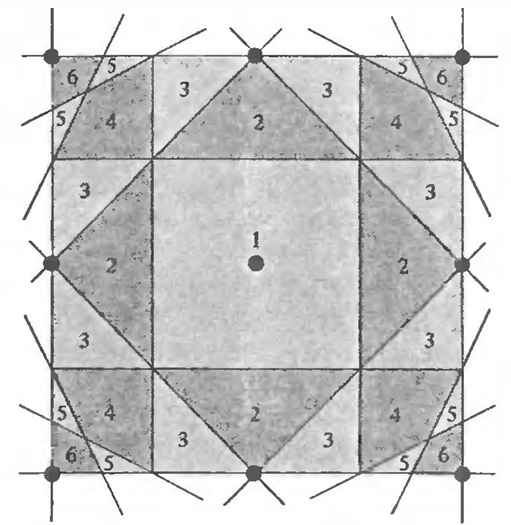
\includegraphics[width=0.4\textwidth]{images/2-Cristalli/BZ.png}
	\caption{queste sono le varie zone di Brillouin in un cristallo e i piani di Bragg sono indicati dale linee}
	\label{fig:BZ}
\end{figure}

in Figura \ref{fig:esBZ} sono riportati degli esempi dove si può osservare l'esterno di varie zone di Brillouin per reticoli FCC e BCC. Allontanandoci dal Piano di Bragg i cambiamenti della struttura elettronica sono deboli mentre vicino ai piani di Bragg sono molto forti, questo concetto è alla base dei gap nei solidi, conoscere le zone di Brillouin è fondamentale per capire la struttura elettronica e le sue interazioni.
\begin{figure} [H]
	\centering
	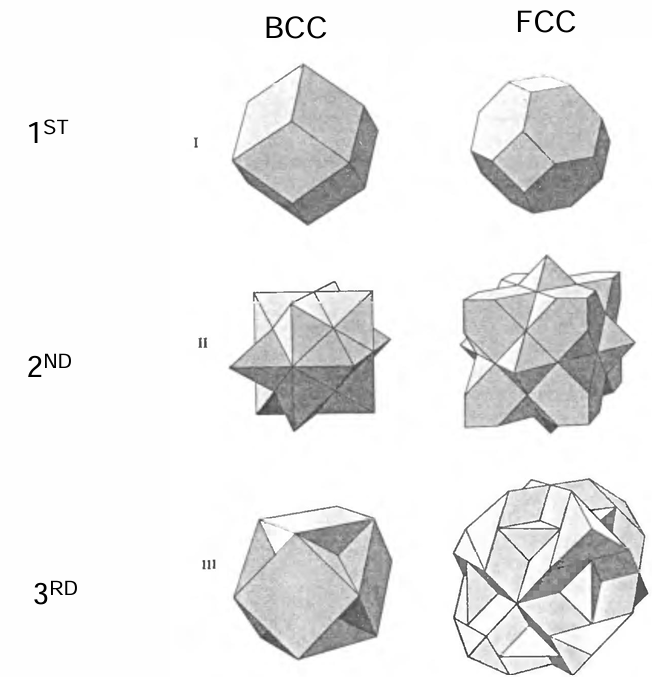
\includegraphics[width=0.45\textwidth]{images/2-Cristalli/esBZ.png}
	\caption{}
	\label{fig:esBZ}
\end{figure}
\section{Piani del reticolo}
Possiamo pensare ad un cristallo come ad una collezione di piani a distanza d, e posso identificare ogni piano con un vettore del reticolo reciproco. \\\\
Per una qualasiasi famiglia di piani cristallini separati da una distanza d, ci sono dei vettori del reticolo reciproco $\mathbf{K}$ perpendicolari al piano , il più corto sarà di lunghezza $\frac{2\pi}{d}$. \\\\
Al contrario, per un qualsiasi vettore del reticolo reciproco $\mathbf{K}$ c'è una famiglia di piani perpendicolari a $\mathbf{K}$ separati da una distanza d dove $\frac{2\pi}{d}$ è la lunghezza del vettore più corto del reticolo reciproco parallelo a K. \\\\
$k_0 = \frac{2\pi}{d}$ ha questa forma perché l'onda piana deve avere lo stesso valore nello spazio k, la dimostrazione di ciò è in Figura \ref{fig:dimpiani}
\begin{figure} [H]
	\centering
	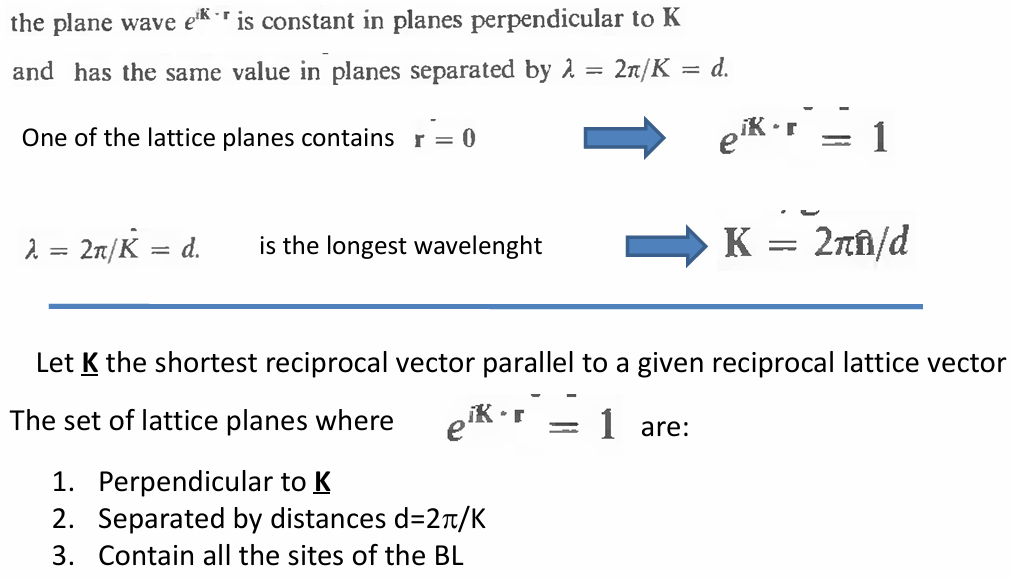
\includegraphics[width=0.9\textwidth]{images/2-Cristalli/dimpiani.png}
	\caption{}
	\label{fig:dimpiani}
\end{figure}

\subsection{Indice di Miller}
Dalla corrispondenza tra i vettori del reticolo reciproco e una famiglia di piani del cristallo possiamo definire un modo più conveniente per specificare l'orientazione del piano. L'\textbf{indice di Miller} di un piano del cristallo sono le coordinate del vettore del reticolo reciproco più corto perpendicolare a quel piano rispetto ad un set di vettori primitivi del reticolo reciproco specifico. Un piano con indici di miller h, k, l è perpendicolare ad un vetorre del reticolo reciproco $hb_1 + kb_2 + lb_3$. Quindi gli indici di Miller sono degli interi e dipendono da una particolare scelta di vettori primitivi. La definizione di indici di Miller è riportata in Figura \ref{fig:indicemiller}
\begin{figure} [H]
	\centering
	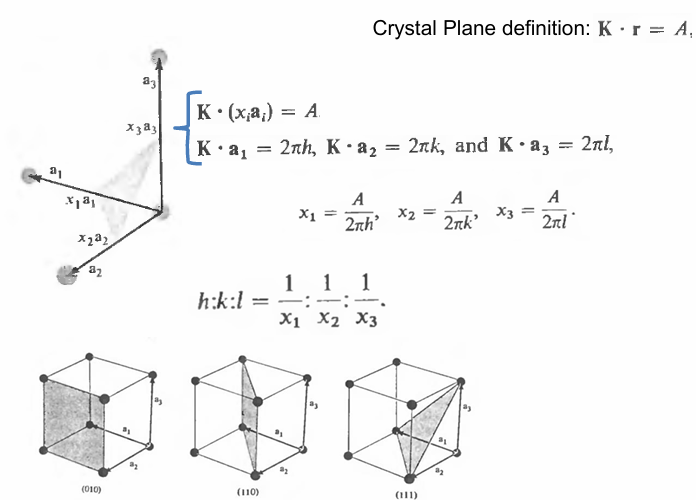
\includegraphics[width=0.9\textwidth]{images/2-Cristalli/indicemiller.png}
	\caption{}
	\label{fig:indicemiller}
\end{figure}

Ci sono diverse notazioni per indicare gli indici di miller una è (001), i piani equivalenti nello spazio reciproco sono $\{ 001 \}$ invece nel piano reale la direzione del cristallo è indicata con $[001]$ e le direzioni equivalenti con $<001>$.

\section{Diffrazione raggi-x nei cristalli e definizione della struttura cristallina}
\subsection{Formulazione di Bragg}
La formulazione di Bragg è un modello che descrive la diffrazione dei raggi X (o di altre onde) da parte di un cristallo, basandosi sull'idea che il cristallo sia costituito da piani reticolari paralleli composti da ioni separati da una distanza $d$ che agiscono come superfici riflettenti.\\\\
Quando un fascio di raggi X incide su un cristallo, esso può essere parzialmente riflesso da strati atomici interni.  L'obbiettivo è comprendere e studiare la posizione dei piani che compongono il solido osservando gli spot generati dalla diffrazione con i raggi X. \\\\
La condizione per cui questi raggi riflessi interferiscono in modo costruttivo è data dalla legge di Bragg:
\[2d\sin\theta = n\lambda\]
con $\theta$ angolo di incidenza detto di Bragg, $n$ numero intero. \\\\
\begin{figure} [H]
	\centering
	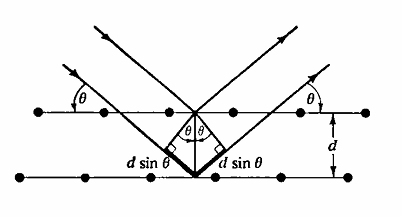
\includegraphics[width=0.4\textwidth]{images/2-Cristalli/braggdiffr.png}
	\caption{rappresentazione grafica della diffrazione, $d\sin \theta$ è la differenza di cammino ottico tra i due raggi riflessi sui diversi piani che determinerà quindi una differenza di fase}
	\label{fig:braggdiffr}
\end{figure}
Limiti:
\begin{itemize}
    \item È una descrizione semplificata che considera il cristallo come una serie di piani paralleli senza tenere conto dell'effetto della diffrazione su scala atomica più fine.
    \item Non include effetti come l'assorbimento dei raggi X o le anomalie legate alla dispersione.
    \item Siccome i piani hanno diverse direzioni ci sarebbe più un $\theta$ da prendere in considerazione.
\end{itemize}



\subsection{Formulazione di Von Laue}
\label{subsec:Formulazione-di-Von-Laue}
IPOTESI:
\begin{enumerate}
    \item Non viene individuata nessuna particolare suddivisione in piani reticolari e non viene imposta nessuna ipotesi di riflessione speculare, ossia non si assume che ogni raggio diffuso da un punto di scattering interferisca in modo costruttivo.\\
    \item Il reticolo è composto da oggetti macroscopici identici posti su dei siti in posizione $\vec{R}$ del B.L. e ciascuno ri-irradia la radiazione in tutte le direzioni.\\
\end{enumerate}
Per ottenere le condizioni di interferenza costruttiva considero uno scattering elastico come in Figura \ref{fig:vonform}, ossia supponiamo che un fascio di raggi X incida su 2 scatteratori posti a distanza $\vec{d}$ con $k$ vettore d'onda incidente e $k'$ vettore d'onda riflesso. 
\begin{figure} [H]
	\centering
	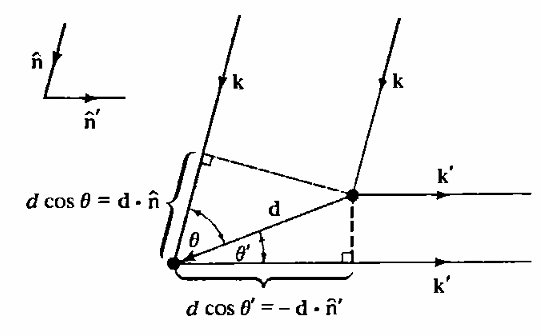
\includegraphics[width=0.5\textwidth]{images/2-Cristalli/vonform.png}
	\caption{}
	\label{fig:vonform}
\end{figure} 

La differenza di cammino ottico è data da:
\[ d\cos \theta + d \cos\theta' = d \cdot (\hat{n} - \hat{n}')\] 
e la condizione per ottenere interferenza costruttiva è:
\[ d \cdot ( \hat{n} - \hat{n}') = m\lambda  \]
siccome lo scattering è elastico avremo che $|k| = |k'|$, moltiplicando da entrambe le parti per $|k| = \frac{2\pi \hat{n}}{\lambda}$ ottengo: 
\[ d \cdot (k - k') = 2\pi m \implies R \cdot (k - k') = 2\pi m \]
poiché d è un vettore del reticolo di reciproco. Quindi guardando ai diversi spot della diffrazione posso ottenere informazioni sul reticolo di Bravais quindi
\[ e^{i(k'-k) \cdot R} = 1\]
confrontando questo risultato con la definizione di reticolo reciproco che è \\ $e^{i K \cdot R} = 1$ arriviamo alla \textbf{condizione di Laue che dice che l'interfenza costruttiva compare provocando un cambiamento nel vettore d'onda pari a $K = k'-k$ che è un vettore del reticolo reciproco}.


Nella condizione in cui $k$ e $k'$ sono uguali prendo $ |k| = |k-K|$ e facendo al quadrato entrambe le parti otteniamo: (ovviamente sono tutti vettori)
\[ \cancel{k^2} =\cancel{ k^2 }+ K^2 - 2k \cdot K \implies  2\vec{k} \cdot \vec{K} = K^2  \implies \frac{1}{K} 2k \cdot K = K^2 \frac{1}{K} \implies \vec{k} \cdot \hat{K} = \frac{1}{2} K\]
\textbf{La componente del vettore incidente k lungo il vettore del reticolo reciproco K deve essere metà della lunghezza di K.}\\\\
La formulazione di Laue è particolarmente utile quando si analizzano pattern di diffrazione complessi, specialmente con sorgenti policromatiche, in cui sono presenti molteplici lunghezze d’onda.
\begin{figure} [H]
	\centering
	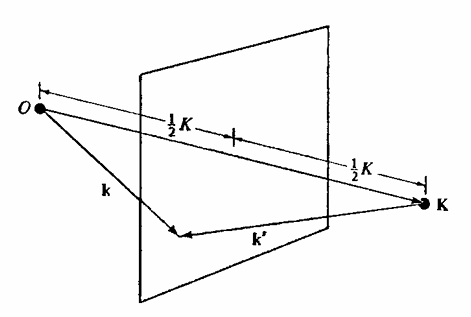
\includegraphics[width=0.5\textwidth]{images/2-Cristalli/vonlaue2.png}
	\caption{}
	\label{fig:vonlaue2}
\end{figure} 

\subsubsection{Equivalenza tra Von Laure e Bragg}
L'equivalenza tra i due criteri segue dalla relazione tra i vettori del reticolo reciproco e le famiglie di piani del cristallo. \\\\
Si supponga che il vettore d'onda incidente k e k' soddisfino la condizione di Laue che dice che $K = k'-k$ è un vettore del reticolo reciproco. Si nota dalla Figura \ref{fig:VLBeq} che k e k' hanno lo stesso angolo $\theta$ con il piano perpendicolare a K. \\
Quindi lo scattering può essere visto come una riflessione di Bragg, con un angolo di Bragg $\theta$ dalla famiglia di piani perpendicolari al vettore del reticolo reciproco K.
\begin{figure} [H]
	\centering
	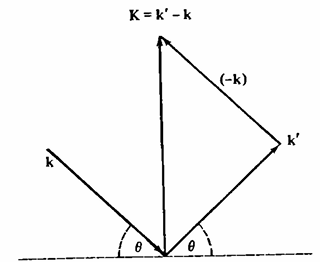
\includegraphics[width=0.5\textwidth]{images/2-Cristalli/VLBeq.png}
	\caption{}
	\label{fig:VLBeq}
\end{figure} 

Per dimostrare che questa affermazione soddisfi la condizione di Bragg, si noti che K è multiplo del vettore del reticolo reciproco più corto parallelo a $\mathbf{K} $
\[\implies K = n K_0 \hspace{0.3cm} \text{siccome} K_0 = \frac{2\pi}{d}\hat{n} \implies K = \frac{2\pi n}{d}\]
Dalla Figura \ref{fig:VLBeq} si osserva anche che $K = 2k \sin \theta$ perciò vale:
\[ k \sin \theta = \frac{\pi n}{d}, \ \ k = \frac{2\pi}{\lambda} \implies n\lambda = 2d\sin \theta \]
Questo significa che Bragg e Von Laue sono equivalenti. \textbf{Quindi la diffrazione di Laue corrisponde ad un cambio nel vettore d'onda dato da un vettore $\mathbf{K}$ del reticolo reciproco che corrisponde ad una riflessione di Bragg da una famiglia di piani del reticolo perpendicolari a \textbf{K}}.

\section{Costruzione di Ewald e metodo di Laue}
Una volta che ho i picchi di diffrazione posso ricostruire la struttura del cristallo ed un modo per farlo è utilizzando il metodo di Ewald che si può osservare in Figura \ref{fig:ewald}, grazie a questo strumento grafico si possono vedere immediatamente quali direzioni del reticolo (cioè quali piani interni al cristallo) genereranno riflessioni costruttive.\\\\
Si disegna una sfera (chiamata sfera di Ewald) con raggio $r = \frac{1}{\lambda} = k$, il centro della sfera è posto alla punta del vettore $k$.
I punti del reticolo reciproco che cadono sulla superficie di questa sfera sono quelli che soddisfano la condizione di diffrazione, siccome non ho mai un fascio monocromatico di Raggi X, ho più spot e quindi delle lunghezze d'onda comprese in un certo intervallo $\lambda_1 < \lambda < \lambda_0$.\\\\
Posso quindi usare i corrispondenti $k_{min}$ e $k_{max}$ per disegnare il cerchio come quello in Figura \ref{fig:metVL}, i picchi di Bragg saranno osservati per ogni vettore del reticolo reciproco compreso nelle sfere di Ewald di raggio $k_1$ e $k_0$.
\begin{figure} [H]
	\centering
	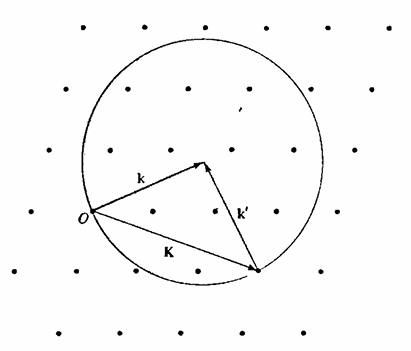
\includegraphics[width=0.5\textwidth]{images/2-Cristalli/ewald.png}
	\caption{}
	\label{fig:ewald}
\end{figure} 
\begin{figure} [H]
	\centering
	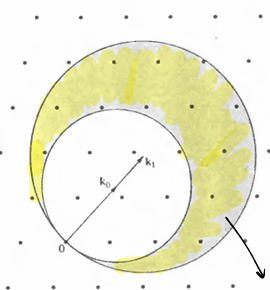
\includegraphics[width=0.5\textwidth]{images/2-Cristalli/metVL.png}
	\caption{L'interferenza si osserverà solo per i punti all'interno dell'area colorata}
	\label{fig:metVL}
\end{figure}

Ruotando il cristallo, ruoto anche il reticolo reciproco, alcuni punti che prima della rotazione non intersecavano la sfera di Edwald in seguito potrebbero farlo (come si osserva in Figura \ref{fig:esEd}) quindi ricostruendo di quanto il cristallo è stato ruotato vedo punti apparire e sparire e posso ricostruire il reticolo reciproco e quindi tornando allo spazio reale descrivere l'orientamento e la simmetria del cristallo.
\begin{figure} [H]
	\centering
	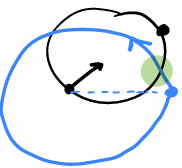
\includegraphics[width=0.3\textwidth]{images/2-Cristalli/esEd.png}
	\caption{Senza ruotare il cristallo il punto considerato non avrebbe intersecato la sfera di edwald}
	\label{fig:esEd}
\end{figure}

\section{Fattore di struttura geometrica }
Possiamo avere la prova che un reticolo sia un reticolo di Bravais semplice oppure uno con base osservando i raggi X? \\
Se è con base l'intensità dei punti non sarà la stessa e questo è dovuto alla presenza del \textbf{fattore geometrico} che è:
\[ S_k = \sum_{j =1}^n e^{i K \cdot d_j} \]
dove j è la posizione dell'atomo, $S_k$ che dipende da K è l'effetto dell'interferenza tra i fasci di raggi X scatterati dal primo e dal secondo atomo, infatti l'intensità del picco cambia con K ed è data da $|S_k|^2$. I raggi x sono la superposizione della diffrazione degli atomi per cella unitaria, negli altri casi c'è interferenza tra 2 atomi della cella. Vedo una modulazione che dipende dalla posizione dei due atomi. \\\\
Ora proviamo a calcolare il Fattore di struttura geometrica per per un BCC considerato come un SC con base riportato in Figura \ref{fig:BCCSC}.
\begin{figure} [H]
	\centering
	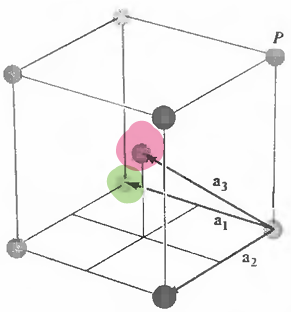
\includegraphics[width=0.3\textwidth]{images/2-Cristalli/BCCSC.png}
	\caption{i punti evidenziati sono $d_1$ e $d_2$}
	\label{fig:BCCSC}
\end{figure}
$d_1 = (0,0,0)$ è il punto nell'angolo mentre $d_2 = \frac{a}{2}(\hat{x}+\hat{y}+\hat{z})$ i vettori del reticolo sono $\Vec{K} = \frac{2\pi}{a}(n_1 \hat{x} + n_2 \hat{y} + n_3 \hat{z})$ per ogni punto del reticolo il fattore di struttura è:
\[ S_k = \sum e^{i \Vec{K}\cdot d_i} = 1 + \exp[i\Vec{K} \cdot \frac{1}{2}(\hat{x}+\hat{y}+\hat{z})] \]
Nel caso in cui i due atomi fossero diversi posso aggiungere un termine $\eta$ 
\[ S_k = 1 +\eta e^{i \pi(n_1 + n_2 + n_3)} = 1 + \eta(-1)^{n_1 + n_2 + n_3} = 
\begin{cases}
1+ \eta, \ n_1 + n_2 + n_3 \ \text{pari} \\
1-\eta, \ n_1 + n_2 + n_3  \ \text{dispari}
\end{cases} \]
Quindi a seconda del punto k ho un'intensità diversa. \\
Invece in un cristallo poliatomico gli ioni nella base non sono identici e quindi ciò che dovrebbe essere $\eta(K)$ dipende da K, quindi il fattore di struttura è:
\[ S_k = \sum_{j = 1}^n f_i(\Vec{K})e^{i K \cdot d_j}  \]
$f_j(K)$ è detto fattore di forma atomica ed è dato da:
\[ f_j(\Vec{K}) = -\frac{1}{e}\int  e^{i \Vec{K} \cdot \Vec{r}} \rho_j(r)\ \d\Vec{r} \]
ed è praticamente la trasformata di Fourier della densità di carica dell'atomo. \\\\

\chapter{Elettroni in un Potenziale Periodico}

Il potenziale in un cristallo possiede la stessa periodicità del reticolo di Bravais, cioè
\[
U(\mathbf{r}) = U(\mathbf{r}+\mathbf{R})\,,
\]
per ogni vettore di traslazione \(\mathbf{R}\).  
Pertanto, l'hamiltoniana del singolo elettrone è:
\begin{equation}
H\psi(\mathbf{r}) = \left[ -\frac{\hbar^2}{2m} \nabla^2 + U(\mathbf{r}) \right]\psi(\mathbf{r}) = \varepsilon\, \psi(\mathbf{r})\,.
\label{eqn:ham}
\end{equation}

\begin{figure}[H]
	\centering
	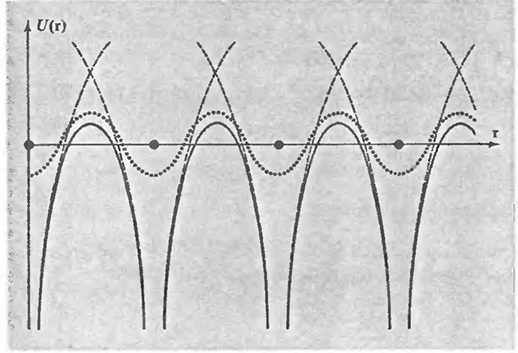
\includegraphics[width=0.5\textwidth]{images/3-Elettroni-Potenziale-Periodico/potper.png}
	\caption{Esempio di potenziale periodico in un cristallo. I punti evidenziati indicano le posizioni degli ioni.}
	\label{fig:potper}
\end{figure}

La periodicità del potenziale è la base per la \emph{teoria a bande} degli elettroni nei solidi, e conduce naturalmente all'uso della funzione d'onda di Bloch:
\[
\psi_{\mathbf{k}}(\mathbf{r}) = e^{i\mathbf{k}\cdot \mathbf{r}} u_{\mathbf{k}}(\mathbf{r})\,,
\]
con \(u_{\mathbf{k}}(\mathbf{r})\) una funzione periodica, cioè \(u_{\mathbf{k}}(\mathbf{r}) = u_{\mathbf{k}}(\mathbf{r}+\mathbf{R})\).

Questa struttura fornisce la base per l'interpretazione sperimentale delle proprietà elettroniche e ottiche dei cristalli.



\section{Teorema di Bloch}
Gli autostati dell'Hamiltoniana di singolo elettrone \ref{eqn:ham} con un potenziale con la stessa periodicità del reticolo di Bravais, sono un'onda piana moltiplicata ad una funzione con la periodicità del reticolo di Bravais
\begin{equation}
\psi_{nk}(r) = e^{i K \cdot r} u_{nk} (r), \ \ u_{nk}(r + R) = u_{nk}(r) \ \ R \in \ \text{BL}
\label{eqn:teobloch}
\end{equation}
$u_{nk}(r)$ in pratica è una funzione di r che è invariante per traslazione lungo i vettori del reticolo di Bravais. 
(\ref{eqn:teobloch}) la posso anche scrivere come:
\[\psi(r + R) = e^{i K \cdot R} \psi(r)\]
mostro che è vero:
\[ \psi(r + R) = e^{i K \cdot (r+R)} u_k(r + R) = e^{iKR}(e^{iKr} u(r)) = e^{i K R} \psi(r) \]
Notiamo anche che se questo è vero allora anche la densità di carica ha la stessa periodicità del reticolo di Bravais:
\[ \rho(r) = |\psi(r)|^2 = |\psi(r)e^{iKR}|^2 = |\psi(r + R)|^2 = \rho(r + R)  \]
all'interno del modulo ho inserito $e^{iKR}$ perché tanto il suo modulo è 1 quindi posso farlo.
\subsection{Dimostrazione del teorema di Bloch}
Per dimostrare il teorema di Bloch utilizzo la formulazione quantistica. \\\\

Definisco l'operatore traslazionale: $T_R f(r) = f(r+R)$\\
\textbf{1: Dimostro che $T_R$ commuta con H}
\[ T_R (H\psi) = H(r + R) \psi(r + R) = H(r) \psi (r+R) = H T_R \psi \implies T_R H = H T_R \]
ho che $H(r+R) = H(r)$ vale perché anche lei è periodica con il periodo del reticolo di Bravais. In ogni caso se $T_R$ ed H commutano questo significa che hanno lo stesso set di autovettori
\[ H\psi = \varepsilon \psi, \ \ T_R \psi = c(R)\psi \]
per il teorema di Bloch i loro autostati saranno:
\[ \psi(r + R) = e^{iKR}\psi(r), \ \ \psi(r + R) = c(R) \psi(r) \]
Dimostrando che queste due sono equivalenti si dimostra il teorema di Bloch. \\
Noto che 
\[ T_{R+R'}\psi(r) = T_R T_{R'} \psi(r) = T_{R'} T_{R} \psi(r) = \psi(r + R + R') \implies T_R T_{R'} =  T_{R'} T_{R} = T_{R+R'} \]
Perciò se 
\[ T_{R'}T_{R}\psi = c(R)T_{R'}\psi = c(R)c(R') \psi \ , \ T_{R'}T_{R} \psi = T_{R + R'} \psi = c(R + R')\psi \]
quindi
\begin{equation}\label{eqn:propcR}  
    c(R + R') = c(R)c(R')
\end{equation}
$T_{R}$ è un operatore unitario quindi il modulo $|c(R)|$ deve essere 1 perché è solo una traslazione e non cambia nessun altra cosa. Quindi con $R = n_1 a_1 + n_2 a_2 + n_3 a_3$ e sapendo che $T_{R} = T_{n_1 a_1 + n_2 a_2 + n_3 a_3}$ usando la proprietà \ref{eqn:propcR} ottengo:
\[ c(R) = C(a_1n_1)c(a_2n_2)c(a_3n_3) = c(a_1)^{n_1}c(a_2)^{n_2}c(a_3)^{n_3} \]
elevo alla $n_1$ perché moltiplico $n_1$ volte la stessa cosa. Se il modulo di $|c(R)|$ deve essere pari a 1 allora $c(R)$ deve essere della forma $c(R) = e^{i\mu}$ quindi in questo caso
\[ c(a_i) = e^{i2\pi x_i} \longrightarrow c(R) = e^{i2\pi(x_1n_1)}e^{i2\pi(x_2n_2)}e^{i2\pi(x_3n_3)} = e^{i 2\pi (x_1 n_1 + x_2n_2 + x_3 n_3)}   \]
sappiamo che $k = (x_1 b_1 + x_2b_2 + x_3 b_3)$ questo vuol dire che 
\[ C(R) = e^{i k \cdot R} \]
perché se $R = n_1 a_1 + n_2 a_2 + n_3 a_3$ e $K = x_1 b_1 + x_2b_2 + x_3 b_3$ allora facendo il prodotto scalare ho che $a_i \cdot b_j = 2\pi \delta_{ij}$ quindi $K \cdot R = 2\pi (x_1 n_1 + x_2n_2 + x_3 n_3)$ perciò
\[ T_R \psi = \psi (r + R) = c(R) \psi = e^{i K\cdot R} \psi (r) \]
Ed è il teorema di Bloch.

\subsection{Dimostrazione teorema di Bloch con trasformata}
Espandiamo la funzione d'onda e il potenziale come:
\[\psi(\mathbf{r})= \sum_q C_q\cdot e^{i\mathbf{q}\cdot \mathbf{r}} \hspace{0.3cm} U(\mathbf{r})= \sum_k U_k\cdot e^{i\mathbf{k}\cdot \mathbf{r}}\]
Con $\mathbf{r}$ vettore del B.L. e $\mathbf{k}$ vettore del R.L.\\\\
Dimostriamo che la trasformata del potenziale $U_k = U^*_k = U_{-k}$:
\[U_k = \int U(\mathbf{r}) \cdot e^{-i\mathbf{k}\cdot \mathbf{r}}\d\mathbf{r} \implies U^*_k = \int U^*(\mathbf{r}) \cdot e^{i\mathbf{k}\cdot \mathbf{r}}\d\mathbf{r} =  \int U(\mathbf{r}) \cdot e^{-i(-\mathbf{k})\cdot \mathbf{r}}\d\mathbf{r} = U_{-k}\]
Per $U(\mathbf{r}) = U(-\mathbf{r})$ si ottiene:
\begin{align*}
	U_k &= \int U(\mathbf{r}) \cdot e^{-i\mathbf{k}\cdot \mathbf{r}}\ \d\mathbf{r} \hspace{0.2cm}\text{invertiamo} \hspace{0.2cm} \mathbf{r} \to -\mathbf{r} \implies\\ 
	\implies U_k &= \int U(\mathbf{r}) e^{-i(\mathbf{-k})\cdot \mathbf{r}}\ \d\mathbf{r}= U_{-k} = U_k^*
\end{align*}
Ora risolviamo l'equazione agli autovalori:\\\\
\begin{enumerate}
    \item Termine cinetico :
    \[-\frac{\hbar^2\nabla^2}{2m}\cdot \psi(\mathbf{r)} =-\frac{\hbar^2\nabla^2}{2m}\cdot \sum_q C_q\cdot e^{i\mathbf{q}\cdot \mathbf{r}} = \frac{\hbar^2}{2m}\sum_q q^2 \cdot C_q\cdot \cdot e^{i\mathbf{q}\cdot \mathbf{r}}\]
    \item Termine potenziale :
    \[U(\mathbf{r}) \cdot \psi(\mathbf{r}) = \sum_{k,q} C_q U_k e^{i(\mathbf{k}+\mathbf{q})\cdot \mathbf{r}}\]
    Sostituiamo $\mathbf{q'} = \mathbf{q}+\mathbf{k}$
    \[U(\mathbf{r}) \cdot \psi(\mathbf{r}) = \sum_{k,q'} C_{q'-k} U_k e^{i\mathbf{q'\cdot r}}\]
    Usiamo il fatto che la scelta del indice è arbitraria (indice muto) ed otteniamo:
    \[U(\mathbf{r}) \cdot \psi(\mathbf{r}) = \sum_q \sum_k C_{q-k} U_k e^{i\mathbf{q\cdot r}}\]
\end{enumerate}
Da cui l'equazione diventa:
\[\frac{\hbar^2}{2m}\sum_q q^2 \cdot C_q\cdot \cdot e^{i\mathbf{q}\cdot \mathbf{r}}+ \sum_q \sum_k C_{q-k} U_k e^{i\mathbf{q\cdot r}} = \varepsilon \cdot \sum_q C_q\cdot e^{i\mathbf{q}\cdot \mathbf{r}}\]
\[\sum_q e^{i\mathbf{q}\cdot \mathbf{r}} \cdot \bigl[\biggr(\frac{\hbar^2}{2m}\cdot \mathbf{q}^2 -\varepsilon\biggr)C_q + \sum_{k} U_k C_{q-k}\bigr]= 0\]
Siccome $\{\mathbf{q}\}$ è un set di vettori orto-normali che soddisfano le Born Van-Karman Conditions, possiamo imporre a zero ciascun coefficiente ed ottenere per $\mathbf{q} = \mathbf{k}- \mathbf{K}$ e $\mathbf{k'}= \mathbf{k}+\mathbf{K}$ con $\mathbf{k}$ vettore della prima zona di brillouin e $\mathbf{K}$ vettore del R.L.
\[\biggr(\frac{\hbar^2}{2m}\cdot (\mathbf{k-K})^2 -\varepsilon\biggr)C_{k-K} + \sum_{k'} U_{k'-K} C_{k-k'}= 0\]
Abbiamo quindi un sistema di n equazioni per ogni valore di $\mathbf{k}$ permesso appartenente alla prima zona di Briollouin, da cui la funzione d'onda può essere riscritta come:
\[\psi(\mathbf{r}) = \sum_q C_q e^{i\mathbf{q}\cdot\mathbf{r}} = \sum_K C_{k-K}e^{i(\mathbf{k}-\mathbf{K})\cdot \mathbf{r}} =e^{i\mathbf{k}\cdot\mathbf{r}} \cdot  \sum_K C_{k-K}e^{-i\mathbf{K}\cdot \mathbf{r}} = e^{i\mathbf{k}\cdot\mathbf{r}} \cdot u_k(\mathbf{r}) \]
\section{Condizioni di Born-Von Karman}
Sono delle condizioni al contorno periodiche:
\[ \psi(r + N_i a_i) = \psi(r) \ , \ i = 1,2,3 \]
$N_i a_i$ è il numero di celle nel solido in ogni direzione e gli $a_i$ sono i vettori primitivi. Per il teorema di Bloch
\[ \psi_{nk}(r + N_i a_i) = e^{i N_i k \cdot a_i} \psi_{nk}(r) \]
ma abbiamo bisogno che $e^{i N_i k \cdot a_i} = 1$ per soddisfare la condizione di periodicità. Quindi se $k = x_1 b_1 + x_2b_2 + x_3 b_3$ allora ho che 
\[  e^{i N_i k \cdot a_i}  =  e^{i 2 \pi N_i x_i} = 1 \implies x_i = \frac{m_i}{N_i} \]
ed è discreto, è un intero diviso per il numero di celle in quella direzione i.\\\\ 
La forma generale del vettore d'onda quindi è:
\[ k = \sum_{i = 1}^3 \frac{m_i}{N_i}b_i \]
Questo significa che il fatto che la lunghezza di un reticolo è limitata causa la discretizzazione dei vettori k. \\\\
Quanti stati sono permessi? \\
Il volume dello spazio k per ogni k permesso è dato da, dato $k =  \frac{m_1}{N_1}b_1 + \frac{m_2}{N_2}b_2 + \frac{m_3}{N_3} b_3$ (ricordando che N è il numero di celle in quella direzione): 
\[ \Delta k = \frac{b_1}{N_1} \cdot \left( \frac{b_2}{N_2} \times \frac{b_3}{N_3} \right) = \frac{1}{N} b_1 \cdot (b_2 \times b_3) \]
quindi $b_1 \cdot (b_2 \times b_3)$ è il volume di un solido costituito da 3 vettori non collineari quindi è il volume della cella primitiva del reticolo reciproco. \\
Il numero di vettori d'onda permessi in una cella primitiva del reticolo reciproco è uguale al numero di siti nel cristallo, $\rho$ è la densità di sttai nel k-space
\[ \Delta k = \frac{(2\pi)^3}{a^3 } = \frac{(2\pi)^3}{V} \hspace{2cm} \rho = \frac{V}{(2\pi)^3} \]
\subsubsection{commenti sul teorema di Bloch}
1) $\psi_{nk}$ \textbf{non è un autostato del momento} $\vec{p} = (\frac{\hbar}{i})\vec{\nabla}$ 
\begin{equation*}
\frac{\hbar}{i} \vec{\nabla} \psi_{nk} = \frac{\hbar}{i} \vec{\nabla}(e^{i k \cdot r} u_{nk}(r)) = \hbar k \psi_{nk} + e^{i k\cdot r} \frac{\hbar}{i} \vec{\nabla} u_{nk}(r)
\end{equation*}
Dovremmo vedere k come un numero quantico caratteristico della simmetria traslazionale di un potenziale periodico, come il momento p che è un numero quantico caratteristico dell'intera simmetria traslazionale dello spazio libero. \\\\
2) se $k$ è confinato alla prima zona di Brillouin e $k'$ è al di fuori della prima zona di Brillouin, allora posso scrivere 
\[\mathbf{k' = k + K}\]
dove $K$ è un vettore del reticolo reciproco, infatti: 
\[ \psi(r + R) = e^{ik' \cdot R}\psi(r) = e^{i k \cdot R + iK \cdot R} \psi(r) = e^{i k \cdot R}\psi(r) \]
3) \textbf{La funzione d'onda dipende da un indice discreto $\mathbf{n}$ e da un continuo $\mathbf{k}$ appartenente alla prima zona di Brillouin}.\\\\
Data l'equazione di Schrodinger 
\[ H\psi = \left( -\frac{\hbar^2}{2m}\nabla^2 + U(r) \right) \psi = \varepsilon \psi \]
con delle funzioni d'onda di Bloch 
\[ \psi(r) = e^{i k \cdot r} u(r) \]
ottengo 
\[ H_k u_k = \left( -\frac{\hbar^2}{2m} \left( \frac{1}{i}\vec{\nabla} + k \right)^2 + U(r) \right) u_k(r) = \varepsilon_k u_k(r) \]
ricordando che $u_k(r) = u_k(r+R)$ \\
Per le condizioni periodiche al contorno, il problema è ristretto ad una sola cella del cristallo, siccome il volume è fissato ci aspettiamo per ogni valore $k$ che l'equazione di schrodinger abbia una \textbf{famiglia infinita di soluzioni con autovalori discreti di indice} $\mathbf{n}$ (come nel caso del elettrone libero in una scatola, ho livelli quantizzati).\\\\
4) \textbf{Periodicità dell'energia e indice di banda.}\\
Posso assegnare gli indici $\mathbf{n}$ ai livelli in modo tale che per un dato $\mathbf{n}$ gli autostati e gli autovalori sono funzioni periodiche in $\mathbf{k}$ del reticolo reciproco (c'è solo $\mathbf{n}$ perché nella nostra trattazione non viene considerata l'interazione con gli spin)
\[ \psi_{n,k}(r + R) = e^{i k \cdot R} \psi_{n,k}(r) \]
\[ \psi_{n, k + K}(r )= \psi_{nk}(r) \]
\[ \varepsilon_{n, k + K}(r )= \varepsilon_{nk}(r) \]
se $\psi$ è periodico nello spazio k allora lo sarà anche l'energia. $\varepsilon_n (k)$ è detta \textbf{banda di energia} ed $\mathbf{n}$ è l'indice della banda. È una banda perché se l'energià è periodica in $\mathbf{k}$ e continua avrà un limite superiore ed uno inferiore, quindi i livelli energetici sono compresi tra questi due limiti. \\\\
5) \textbf{Velocità}\\
Un elettrone in un livello specificato dall'indice di banda n e con vettore d'onda k ha una velocità data da:
\[ v_n (k) = \frac{1}{\hbar} \nabla_k \varepsilon_n (k) \]
$v_n(k)$ è la velocità di un pachetto d'onda, si nota che la velocità di un elettrone è in relazione al gradiente dell'energia questo perché è limitata, ci sono punti dove la velocità sarà 0 perché lo sarà anche il gradiente. 
\begin{figure} [H]
	\centering
	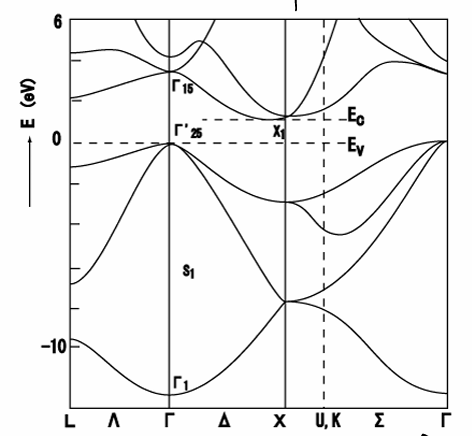
\includegraphics[width=0.5\textwidth]{images/3-Elettroni-Potenziale-Periodico/esbande.png}
	\caption{esempio di bande in un cristallo FCC. le bande vengono riempire sempre seguendo il principio di esclusione di Pauli}
	\label{fig:esbande}
\end{figure}

\subsection{Superficie di Fermi}
Siccome le bande vengono riempite sempre seguendo il principio di esclusione di Pauli un certo numero di bande può essere completamente pieno e altre invece possono rimanere vuote, la differenza di energia tra il livello occupato più alto e il livello non occupato più basso è detto \textbf{gap}. \\
Un certo numero di bande invece potrebbe essere parzialmente pieno e per ogni banda di questo tipo ci sarà una superficie nello spazio k che separa i livelli occupati da quelli non occupati. L'insieme di tutte queste superfici è noto come \textbf{superificie di Fermi}, ed è una generalizzazione degli elettroni liberi nella sfera di Fermi al modello di Bloch. \\
$\varepsilon_n(k) = \varepsilon_F$ definisce la superificie di Fermi

\subsection{Densità di stati}
Ora ho una serie di bande che contribuiscono in maniera diversa alla densità degli stati, quindi la densità di stati dipenderà da n. \\
Ciò che dovrò fare sarà calcolare una quantità che è una somma pesata  sui livelli elettronici di diverse proprietà di un singolo elettrone, e queste quantità sono del tipo:
\[ Q = 2 \sum_{n,k} Q_n (k) \]
Per ogni n la somma è su tutti i k permessi dando livelli distinti. Nel limite di un cristallo molto grande i valori permessi dei k si infittiscono diventando sempre più vicini tra di loro, quindi al posto della somma posso integrare. Dato che il volume dello spazio k per k permesso ha lo stesso valore del caso in cui l'elettrone è libero, tutto ciò che è stato ottenuto nel caso dell'elettrone libero rimane valido:
\begin{equation} q = \lim_{v \to \infty} \frac{Q}{V} = 2 \sum_n \int \frac{\d{k}}{(2\pi)^3} Q_n(k) \label{eqn:q1} \end{equation}
$Q_n (k)$ dipende da n e k solo attraverso l'energia $\varepsilon_n(k)$, qundi sempre seguendo l'analogia col caso con l'elettrone libero uno può definire la densità di stati per unità di volume per unità di volume $g(\varepsilon)$ in modo che q abbia la forma:
\begin{equation}\label{eqn:q2}
    q = \int \d{\varepsilon} g(\varepsilon)Q(\varepsilon)
\end{equation}
confrontando \ref{eqn:q1} e \ref{eqn:q2} trovo che 
\[ g(\varepsilon) = \sum_n g_n (\varepsilon) \]
con l'introduzione di questa definizione di densità di stati
\[ g_n (\varepsilon) = \int \frac{\d{k}}{4\pi^3}\delta(\varepsilon - \varepsilon_n(k)) \]
che indica il numero di stati compreso tra $\varepsilon$ ed $\varepsilon_n$. \\
Se voglio trovare anche l'energia totale
\[ U = \sum_{k,n} \varepsilon_n(R) f(T, \varepsilon_n(R)) \]
dove $\varepsilon_n(R)$ è una funzione di $Q_n(k)$ ed $f(T, \varepsilon_n(R))$ è la distribuzione di Fermi Dirac. \\
Un altro modo per rappresentare la densità di stati è riportato nelle figure \ref{fig:densst1} e \ref{fig:densst2} e si fa comportandoci come nel caso dell'elettrone libero. 
\begin{figure}[H]
	\centering
	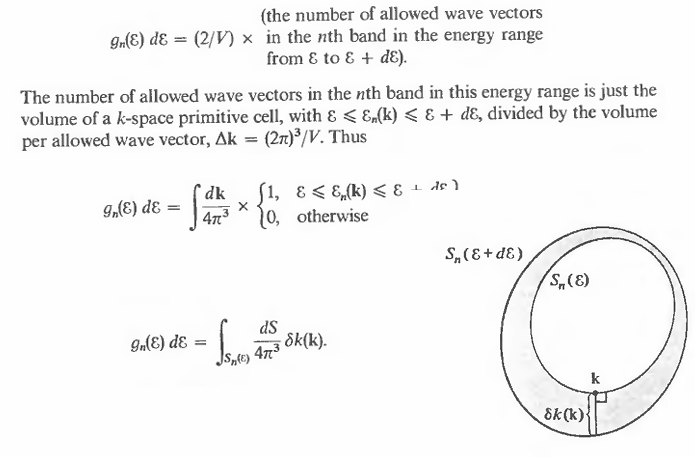
\includegraphics[width=\textwidth]{images/3-Elettroni-Potenziale-Periodico/densst1.png}
	\caption{}
	\label{fig:densst1}
\end{figure}
\begin{figure}[H]
	\centering
	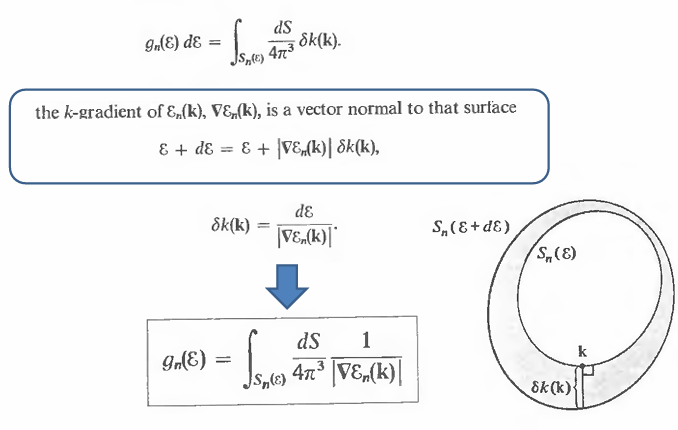
\includegraphics[width=\textwidth]{images/3-Elettroni-Potenziale-Periodico/densst2.png}
	\caption{}
	\label{fig:densst2}
\end{figure} 


\chapter{Elettroni in un Potenziale Debole}

\section{Nearly-Free Electron Approximation}
In questa approssimazione il potenziale \( U(\mathbf{r}) \) tra gli elettroni e gli ioni è considerato debole. Le ragioni per poter adottare questo modello sono le seguenti:
\begin{itemize}
	\item L'interazione ione--elettrone è forte quando i due sono molto vicini, ma agli elettroni in conduzione non è permesso avvicinarsi troppo allo ione perché la regione attorno allo ione è già occupata dagli elettroni di core.
	\item Nella regione in cui sono permessi gli elettroni in conduzione la loro elevata mobilità permette uno screening efficace del campo generato dagli ioni, riducendo il potenziale netto che ciascun elettrone "sente".
\end{itemize}
Poiché il potenziale è debole, lo trattiamo come una perturbazione.
La funzione d'onda di Bloch si scrive come:
\[
\psi_{\mathbf{k}}(\mathbf{r}) = \sum_{K} c_{\mathbf{k}-\mathbf{K}}\, e^{i (\mathbf{k}-\mathbf{K})\cdot \mathbf{r}}\,,
\]
dove la somma viene effettuata su tutti i vettori del reticolo reciproco \(\mathbf{K}\).
I coefficienti \(c_{\mathbf{k}-\mathbf{K}}\) e l'energia \(\varepsilon\) sono determinati dall'hamiltoniana perturbata:
\begin{equation}
\left[ \frac{\hbar^2}{2m} (\mathbf{k} - \mathbf{K})^2 - \varepsilon \right] c_{\mathbf{k}-\mathbf{K}} + \sum_{K'} U_{\mathbf{K'}- \mathbf{K}} \, c_{\mathbf{k}-\mathbf{K'}} = 0\,.
\label{eqn:hampotdebole}
\end{equation}
La parte di perturbazione, dovuta al potenziale debole, è data dal termine:
\begin{equation}
\sum_{K'} U_{\mathbf{K'}- \mathbf{K}} \, c_{\mathbf{k}-\mathbf{K'}}\,.
\label{eqn:perturbazione}
\end{equation}
1) Per prima cosa risolviamo il \textbf{caso non perturbato, cioè per gli elettroni liberi}. \\
In assenza di \(U\) l'hamiltoniana si riduce a:
\[
\left[ \frac{\hbar^2}{2m}(\mathbf{k}-\mathbf{K})^2 - \varepsilon \right] c_{\mathbf{k}-\mathbf{K}} = 0\,.
\]
Definiamo l'energia degli elettroni liberi come:
\begin{equation}
\varepsilon^0_{\mathbf{q}} = \frac{\hbar^2 q^2}{2m}\,,
\label{eqn:enimpert}
\end{equation}
con \(\mathbf{q} = \mathbf{k} - \mathbf{K}\).
Pertanto, in assenza di perturbazione, l'equazione si scrive:
\[
(\varepsilon^0_{\mathbf{k}-\mathbf{K}} - \varepsilon)\, c_{\mathbf{k}-\mathbf{K}} = 0\,.
\]
Da questa equazione emergono due possibili soluzioni:
\begin{enumerate}
	\item \(c_{\mathbf{k}-\mathbf{K}} = 0\);
	\item Oppure \(\varepsilon = \varepsilon^0_{\mathbf{k}-\mathbf{K}}\).
\end{enumerate}
Nel caso \textbf{non degenere}, per un dato \(\mathbf{k}\) esiste un solo vettore \(\mathbf{K}_1\) per cui \(\varepsilon = \varepsilon^0_{\mathbf{k}-\mathbf{K}_1}\) e la funzione d'onda è proporzionale a \( e^{i(\mathbf{k}-\mathbf{K}_1)\cdot \mathbf{r}}\). \\\\

2) Nel caso \textbf{degenere} invece, si ha che per alcuni \(\mathbf{k}\) esistono più vettori del reticolo reciproco, \(\mathbf{K}_1, \ldots, \mathbf{K}_m\), tali che
\[
\varepsilon^0_{\mathbf{k}-\mathbf{K}_1} = \cdots = \varepsilon^0_{\mathbf{k}-\mathbf{K}_m}\,.
\]
In questo caso la soluzione è una combinazione lineare di onde piane:
\[
\psi_{\mathbf{k}}(\mathbf{r}) = \sum_{i=1}^{m} c_{\mathbf{k}-\mathbf{K}_i}\, e^{i(\mathbf{k}-\mathbf{K}_i)\cdot \mathbf{r}}\,.
\]
Poiché l'energia degli elettroni liberi è data dalla parabola \(\varepsilon^0_{\mathbf{q}} = \frac{\hbar^2 q^2}{2m}\), si ottengono delle parabole centrate in ciascun \(\mathbf{K}\) (vedi figura~\ref{fig:solpotdebole}).\\
L'unica soluzione indipendente si ottiene, per convenienza, nella prima zona di Brillouin, mentre i punti in cui due parabole si intersecano sono dei punti di degenerazione.

\begin{figure}[H]
	\centering
	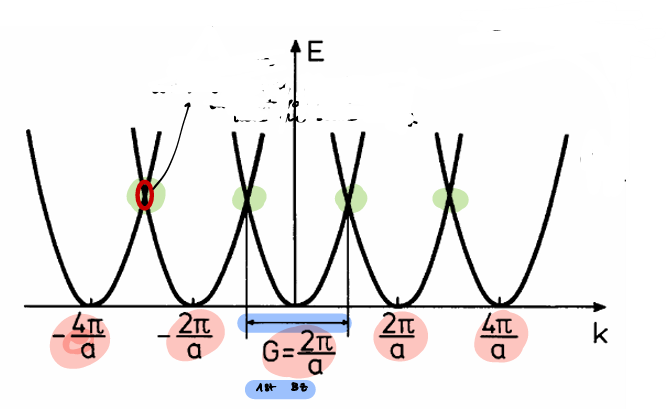
\includegraphics[width=\textwidth]{images/4-Elettroni-Potenziale-Debole/soluzpotdebole.png}
	\caption{Soluzioni imperturbate (onde piane) per il potenziale debole: parabole centrate in ciascun vettore \(\mathbf{K}\). I punti di intersezione rappresentano degenerazioni.}
	\label{fig:solpotdebole}
\end{figure}


\subsection{Effetti della Perturbazione Debole: Due Casi}
Quando il potenziale \(U\) non è più nullo occorrono correzioni all'energia e ai coefficienti \(c_{\mathbf{k}-\mathbf{K}}\).  
Esaminiamo due casi distinti:
\subsubsection{Caso A: Senza Degenerazione}

Fissato un certo \(\mathbf{k}\), supponiamo che esista un vettore \(\mathbf{K}_1\) tale che l'energia imperturbata \(\varepsilon^0_{\mathbf{k}-\mathbf{K}_1}\) sia ben separata (in termini dell'ordine di grandezza di \(U\)) da tutti gli altri livelli \(\varepsilon^0_{\mathbf{k}-\mathbf{K}}\) per ogni \(\mathbf{K} \neq \mathbf{K}_1\).  
Formalmente, si assume che
\begin{equation}
|\varepsilon^0_{\mathbf{k}-\mathbf{K}_1} - \varepsilon^0_{\mathbf{k}-\mathbf{K}}| \gg |U| \quad \text{per ogni } \mathbf{K} \neq \mathbf{K}_1\,.
\label{eqn:casoA}
\end{equation}
In questo caso la soluzione imperturbata è:
\[
\varepsilon = \varepsilon^0_{\mathbf{k}-\mathbf{K}_1}, \quad c_{\mathbf{k}-\mathbf{K}_1} \neq 0, \quad c_{\mathbf{k}-\mathbf{K}} = 0 \quad \text{per } \mathbf{K} \neq \mathbf{K}_1\,.
\]
Inserendo \( \mathbf{K} = \mathbf{K}_1 \) in \eqref{eqn:hampotdebole} si ottiene:
\begin{equation}
\bigl(\varepsilon - \varepsilon^0_{\mathbf{k}-\mathbf{K}_1}\bigr)c_{\mathbf{k}-\mathbf{K}_1} = \sum_{\mathbf{K}} U_{\mathbf{K} - \mathbf{K}_1} \, c_{\mathbf{k}-\mathbf{K}}\,.
\label{eqn:eq1}
\end{equation}
Si ricorda che la costante additiva del potenziale è scelta in modo tale che \(U_{\mathbf{0}} = 0\); pertanto, nel lato destro appariranno solo termini con \(\mathbf{K} \neq \mathbf{K}_1\).

Per \(\mathbf{K} \neq \mathbf{K}_1\), si può risolvere l'equazione \eqref{eqn:hampotdebole} per \(c_{\mathbf{k}-\mathbf{K}}\):
\[ c_{k - K} = \frac{U_{\mathbf{K}_1 - \mathbf{K}}\,c_{\mathbf{k}-\mathbf{K}_1}}{\varepsilon - \varepsilon^0_{\mathbf{k}-\mathbf{K}}}  + \sum_{K' \neq K_1}\frac{U_{K'-K}c_{k - K'}}{\varepsilon - \varepsilon^0_{k - K}}c_{\mathbf{k}-\mathbf{K}} = \frac{U_{\mathbf{K}_1 - \mathbf{K}}\,c_{\mathbf{k}-\mathbf{K}_1}}{\varepsilon - \varepsilon^0_{\mathbf{k}-\mathbf{K}}} + O(U^2)\]
Poiché per il caso non degenere (secondo l'ipotesi in \eqref{eqn:casoA}) \(\varepsilon^0_{\mathbf{k}-\mathbf{K}}\) è ben distante da \(\varepsilon^0_{\mathbf{k}-\mathbf{K}_1}\), i termini \(c_{\mathbf{k}-\mathbf{K}}\) risultano di ordine \(U\).  \\\\
Sostituendo nell'equazione per \(\mathbf{K} = \mathbf{K}_1\) in \eqref{eqn:eq1} si ottiene:
\[
\bigl(\varepsilon - \varepsilon^0_{\mathbf{k}-\mathbf{K}_1}\bigr)c_{\mathbf{k}-\mathbf{K}_1} = \sum_{\mathbf{K}\neq \mathbf{K}_1} U_{\mathbf{K} - \mathbf{K}_1}\, \frac{U_{\mathbf{K}_1-\mathbf{K}}\,c_{\mathbf{k}-\mathbf{K}_1}}{\varepsilon - \varepsilon^0_{\mathbf{k}-\mathbf{K}}} + O(U^3)\,.
\]
Dividendo per \(c_{\mathbf{k}-\mathbf{K}_1}\) (non nullo) e risolvendo per \(\varepsilon\) con le opportune simmetrie $U_k = U_{-k}= U^*_k$, si ottiene la correzione al secondo ordine:
\[
\varepsilon = \varepsilon^0_{\mathbf{k}-\mathbf{K}_1} + \sum_{\mathbf{K}\neq \mathbf{K}_1} \frac{|U_{\mathbf{K}_1-\mathbf{K}}|^2}{\varepsilon^0_{\mathbf{k}-\mathbf{K}_1} - \varepsilon^0_{\mathbf{k}-\mathbf{K}}} + O(U^3)\,.
\]
Questa espressione mostra che le bande non degenere subiscono uno spostamento (o "repulsione") perturbativo:  
i livelli imperturbati inferiori (con denominatore positivo) contribuiscono ad aumentare \(\varepsilon\) mentre quelli superiori (con denominatore negativo) tendono a diminuirla.
\begin{figure}[H]
	\centering
	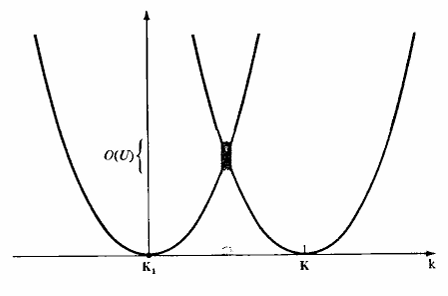
\includegraphics[width=0.5\textwidth]{images/4-Elettroni-Potenziale-Debole/seplivU.png}
	\caption{Intervallo di \(k\) in cui i livelli di energia imperturbati \(\varepsilon^0_{\mathbf{k}-\mathbf{K}_1}\) e \(\varepsilon^0_{\mathbf{k}-\mathbf{K}}\) differiscono di un termine dell'ordine \(O(U)\).}
	\label{fig:seplivU}
\end{figure}


\subsubsection{Caso B: Caso Degenere}
Supponiamo ora che, per un certo \(\mathbf{k}\), esistano \(m\) vettori del reticolo reciproco \(\mathbf{K}_1, \ldots, \mathbf{K}_m\) tali che:
\[
\varepsilon^0_{\mathbf{k}-\mathbf{K}_1} = \varepsilon^0_{\mathbf{k}-\mathbf{K}_2} = \cdots = \varepsilon^0_{\mathbf{k}-\mathbf{K}_m}\,,
\]
e che per ogni \(\mathbf{K} \not\in \{\mathbf{K}_1, \ldots, \mathbf{K}_m\}\) si abbia
\[
|\varepsilon^0_{\mathbf{k}-\mathbf{K}} - \varepsilon^0_{\mathbf{k}-\mathbf{K}_i}| \gg |U| \quad \text{per } i=1,\ldots,m\,.
\]
In questo caso le equazioni \eqref{eqn:hampotdebole} per \( \mathbf{K} = \mathbf{K}_i\) (con \(i=1,\ldots,m\)) devono essere trattate insieme.  
Per \(i=1,\ldots,m\) scriviamo:
\begin{equation}
\bigl(\varepsilon - \varepsilon^0_{\mathbf{k}-\mathbf{K}_i}\bigr)c_{\mathbf{k}-\mathbf{K}_i} = \sum_{j=1}^{m} U_{\mathbf{K}_j-\mathbf{K}_i}\, c_{\mathbf{k}-\mathbf{K}_j} + \sum_{\mathbf{K} \notin \{\mathbf{K}_1,\ldots,\mathbf{K}_m\}} U_{\mathbf{K}-\mathbf{K}_i}\, c_{\mathbf{k}-\mathbf{K}}\,,
\label{eqn:eq4}
\end{equation}
mentre per \(\mathbf{K}\) al di fuori dell'insieme degenere abbiamo (come nel caso A):
\begin{equation}
c_{\mathbf{k}-\mathbf{K}} = \frac{1}{\varepsilon - \varepsilon^0_{\mathbf{k}-\mathbf{K}}} \sum_{j=1}^{m} U_{\mathbf{K}_j-\mathbf{K}}\, c_{\mathbf{k}-\mathbf{K}_j} + O(U^2)\,,
\label{eqn:eq3}
\end{equation}
il cui contributo è di ordine \(U\).  
Inserendo \eqref{eqn:eq3} nell'equazione (\ref{eqn:eq4}) per \(i=1,\ldots,m\), il termine perturbativo esterno fornisce contributi di ordine \(U^2\).  
Dal momento che stiamo ricercando gli effetti principali, e considerando che nel limite \(U\to 0\) tale termine diventa trascurabile, trunchiamo al primo ordine ottenendo il sistema lineare:
\begin{equation}
\bigl(\varepsilon - \varepsilon^0_{\mathbf{k}-\mathbf{K}_i}\bigr) c_{\mathbf{k}-\mathbf{K}_i} = \sum_{j=1}^{m} U_{\mathbf{K}_j-\mathbf{K}_i}\, c_{\mathbf{k}-\mathbf{K}_j}, \quad i=1,\ldots,m\,.
\label{eqn:eq6}
\end{equation}
Questo sistema di \(m\) equazioni lineari determina i coefficienti \(c_{\mathbf{k}-\mathbf{K}_i}\) e le energie perturbate \(\varepsilon\) entro il sottospazio di degenerazione.  
L'energia risultante subirà uno spostamento del secondo ordine in \(U\); tuttavia, in questo trattamento di base, il problema si riduce alla diagonalizzazione della matrice perturbativa \(U_{\mathbf{K}_j-\mathbf{K}_i}\) al fine di determinare le correzioni energetiche.

Riassumendo:
\begin{itemize}
	\item Nel \textbf{caso non degenere} (condizione \eqref{eqn:casoA}), l'energia perturbata è data da:
	\[
	\varepsilon = \varepsilon^0_{\mathbf{k}-\mathbf{K}_1} + \sum_{\mathbf{K} \neq \mathbf{K}_1} \frac{|U_{\mathbf{K}_1-\mathbf{K}}|^2}{\varepsilon^0_{\mathbf{k}-\mathbf{K}_1} - \varepsilon^0_{\mathbf{k}-\mathbf{K}}} + O(U^3)\,.
	\]
	\item Nel \textbf{caso degenere}, il problema si riduce a diagonalizzare la matrice perturbativa \(U_{\mathbf{K}_j-\mathbf{K}_i}\) all'interno del sottospazio degenerato, determinando così le energie perturbate e la combinazione lineare degli stati che, in assenza di \(U\), risultavano degenere.
\end{itemize}

Questo trattamento permette di comprendere come il potenziale debole, trattato come perturbazione, modifichi i livelli energetici degli elettroni. Nei casi non degeneri l'effetto della perturbazione compare al secondo ordine, mentre nei casi degenere la struttura degli autostati viene "mista" e si ottengono soluzioni linearmente combinate che eliminano la degenerazione.

\bigskip






\section{Livelli Energetici Vicino ai Piani di Bragg}
In questa sezione si analizzano le soluzioni dell'equazione agli autovalori per elettroni in un potenziale periodico debole, concentrandosi sui casi in cui due livelli dell'elettrone libero sono quasi degeneri, ovvero quando la loro energia imperturbata differisce di un termine dell'ordine di \(U\) (l'ampiezza del potenziale perturbativo), mentre la differenza con gli altri livelli è molto maggiore di \(U\).  
Formalmente, supponiamo che per una certa quantità \(\mathbf{q}\) (dove \(\mathbf{q} = \mathbf{k} - \mathbf{K}_1\)) si abbia
\[
\varepsilon^0_{q} \sim \varepsilon^0_{q-K}\,,
\]
con la condizione che per ogni altro vettore di reticolo \(\mathbf{K'} \neq 0,\) si verifichi:
\[
|\varepsilon^0_{q} - \varepsilon^0_{q-K'}| \gg |U|\,.
\]
Questa condizione si verifica quando
\[
|q| = |q-K|\,,
\]
che è la definizione geometrica di un piano di Bragg.\\
Da ciò possiamo dedurre due affermazioni fondamentali:
\begin{itemize}
	\item Se \(|q| = |q-K|\), allora il punto \(\mathbf{q}\) giace sul piano di Bragg determinato dal vettore di reticolo \(K\).
	\item Se il punto \(\mathbf{q}\) giace sul piano di Bragg, allora il vettore \(\mathbf{q} - \frac{1}{2}\mathbf{K}\) è parallelo al piano.
\end{itemize}
(Per ulteriori dettagli, si veda la sezione denominata “Formulazione di Von Laue”.)\\\\
Le figure in basso mostrano due rappresentazioni grafiche degli stati energetici vicino al piano di Bragg:
\begin{figure}[H]
	\centering
	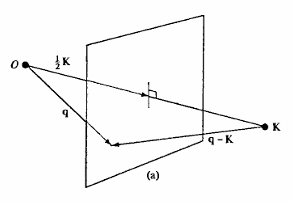
\includegraphics[width=0.4\textwidth]{images/4-Elettroni-Potenziale-Debole/elevelBraggP1.png}
	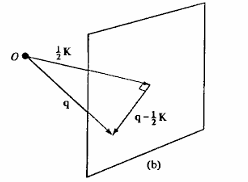
\includegraphics[width=0.4\textwidth]{images/4-Elettroni-Potenziale-Debole/elevelBraggP2.png}
	\caption{Diagrammi schematici dei livelli energetici vicino al piano di Bragg.}
	\label{fig:elevelBraggP}
\end{figure}

\bigskip
\noindent
\textbf{ Ci si aspetta degenerazione al bordo della zona di Brillouin, in quanto i vettori d'onda di elettroni vicini ai piani di Bragg, dove si possono verificare riflessioni di Bragg, sono quelli maggiormente influenzati dal potenziale periodico debole.}\\
\bigskip
\subsection{Struttura dei Livelli quando un Solo Piano di Bragg è Vicino}
Consideriamo il caso in cui un solo piano di Bragg interferisca con i livelli imperturbati. Supponiamo di avere due componenti significative per la funzione d'onda, associate a due vettori del reticolo reciproco \(K_1\) e \(K_2\). In assenza di perturbazione le energie imperturbate sono:
\[
\varepsilon^0_{k-K_1} \quad \text{e} \quad \varepsilon^0_{k-K_2}\,,
\]
ed ipotizziamo che siano quasi degeneri. L'equazione perturbata (vedi equazione \eqref{eqn:hampotdebole} della sezione precedente) assume, per i due termini significativi, la forma:
\[
(\varepsilon - \varepsilon^0_{k-K_1})\,c_{k-K_1} = U_{K_2 - K_1}\,c_{k-K_2}\,,
\]
\[
(\varepsilon - \varepsilon^0_{k-K_2})\,c_{k-K_2} = U_{K_1 - K_2}\,c_{k-K_1}\,.
\]
Per semplificare l'analisi, introduciamo le nuove variabili:
\[
q = k-K_1,\quad \text{e} \quad K = K_2 - K_1\,.
\]
Con queste definizioni, le due equazioni diventano:
\begin{equation}
(\varepsilon - \varepsilon^0_{q})\, c_{q} = U_{K}\, c_{q-K}\,,
\label{eqn:eqBragg}
\end{equation}
\begin{equation}
(\varepsilon - \varepsilon^0_{q-K})\, c_{q-K} = U_{-K}\, c_{q}\,.
\label{eqn:eqBragg2}
\end{equation}
Per trovare le energie permettendo la presenza di due componenti, cerchiamo soluzioni non banali imponendo che il sistema omogeneo di equazioni abbia determinante nullo:
\[
\det \begin{pmatrix}
\varepsilon - \varepsilon^0_{q} & -U_{K} \\
-U_{K}^* & \varepsilon - \varepsilon^0_{q-K}
\end{pmatrix} = 0\,.
\]
Questo determinante fornisce:
\[
(\varepsilon - \varepsilon^0_{q})(\varepsilon - \varepsilon^0_{q-K}) - |U_K|^2 = 0\,.
\]
Risolvendo per \(\varepsilon\) si ottiene:
\begin{equation}
\varepsilon = \frac{1}{2}\left(\varepsilon^0_{q} + \varepsilon^0_{q-K}\right) \pm \sqrt{\left(\frac{\varepsilon^0_{q} - \varepsilon^0_{q-K}}{2}\right)^2 + |U_K|^2}\,.
\label{eqn:soluzioneeps}
\end{equation}
Nel caso particolare in cui il punto \(q\) giaccia sul piano di Bragg, abbiamo
\[
|q| = |q-K| \quad \Rightarrow \quad \varepsilon^0_{q} = \varepsilon^0_{q-K}\,.
\]
Quindi l'equazione \eqref{eqn:soluzioneeps} si semplifica a:
\[
\varepsilon = \varepsilon^0_{q} \pm |U_K|\,.
\]
Questo risultato mostra che, in corrispondenza del piano di Bragg, l'energia si splitta in due valori differenti separati da un gap di ampiezza \(2|U_K|\).\\
Inoltre, ricordando che per un elettrone libero
\[
\varepsilon^0_q = \frac{\hbar^2 q^2}{2m}\,,
\]
si calcola il gradiente dell'energia:
\[
\frac{\partial \varepsilon}{\partial q} = \frac{\hbar^2}{m}\left(q - \frac{1}{2}K\right)\,.
\]
Si osserva che il gradiente risulta parallelo al piano di Bragg (poiché \(K\) è fisso per quel piano).\\\\
\textbf{Determinazione delle Funzioni d'Onda:}
Per il sistema di equazioni \eqref{eqn:eqBragg} e \eqref{eqn:eqBragg2} risulta utile analizzare il rapporto tra i coefficienti \(c_q\) e \(c_{q-K}\).  
Se poniamo:
\[
\varepsilon = \varepsilon^0_q \pm |U_K|\,,
\]
l'equazione \eqref{eqn:eqBragg} diventa (notando che \(\varepsilon - \varepsilon^0_q = \pm |U_K|\)):
\[
\pm |U_K|\, c_{q} = U_K\, c_{q-K}\,,
\]
da cui si ricava:
\[
c_{q} = \pm \frac{U_K}{|U_K|}\, c_{q-K} = \pm \operatorname{sgn}(U_K)\, c_{q-K}\,.
\]
Pertanto, a seconda del segno di \(U_K\), le due soluzioni avranno coefficienti in rapporto:
\begin{itemize}
	\item Per \(U_K>0\):
		\[
		|\psi(r)|^2 \propto \left(\cos\frac{1}{2}K\cdot r\right)^2 \quad \text{per } \varepsilon = \varepsilon^0_q + |U_K|,
		\]
		\[
		|\psi(r)|^2 \propto \left(\sin\frac{1}{2}K\cdot r\right)^2 \quad \text{per } \varepsilon = \varepsilon^0_q - |U_K|.
		\]
	\item Per \(U_K<0\):
		\[
		|\psi(+)|^2 \propto \left(\sin\frac{1}{2}K\cdot r\right)^2 \quad \text{per } \varepsilon = \varepsilon^0_q + |U_K|,
		\]
		\[
		|\psi(-)|^2 \propto \left(\cos\frac{1}{2}K\cdot r\right)^2 \quad \text{per } \varepsilon = \varepsilon^0_q - |U_K|.
		\]
\end{itemize}
La figura~\ref{fig:andamentiUpsi} mostra schematicamente l'andamento delle funzioni d'onda corrispondenti ai due livelli (le soluzioni sono "piccate" rispettivamente sull'atomo e nello spazio tra gli atomi).
\begin{figure}[H]
	\centering
	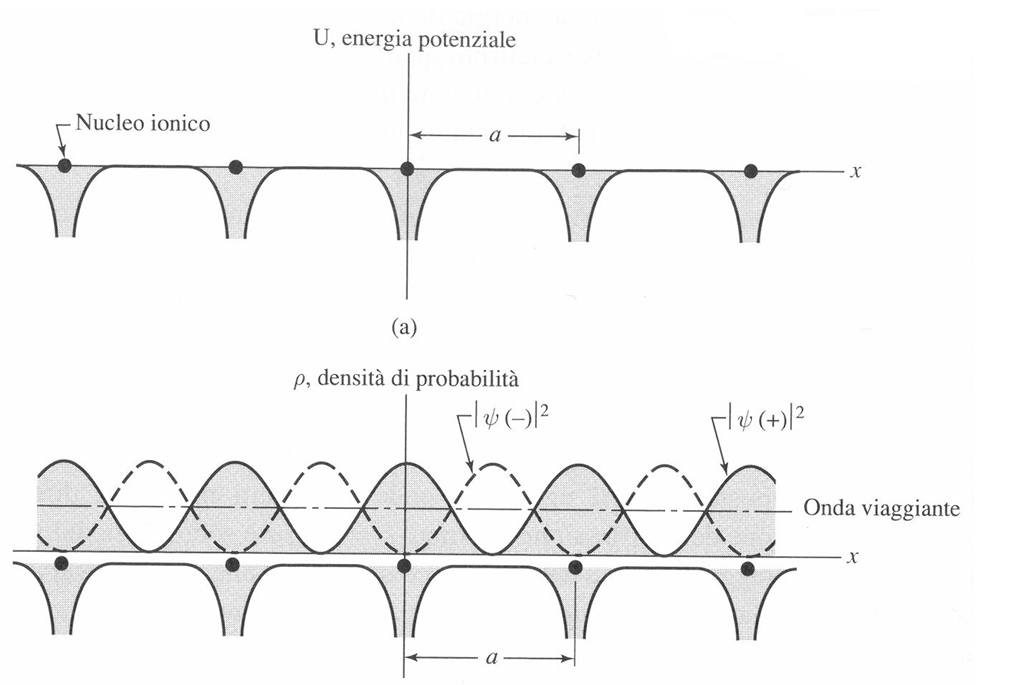
\includegraphics[width=0.8\textwidth]{images/4-Elettroni-Potenziale-Debole/andamentiUpsi.png}
	\caption{Le funzioni d'onda \(|\psi(+)|^2\) e \(|\psi(-)|^2\) per i due livelli splitati. La soluzione \(|\psi(+)|^2\) presenta massimo di densità sull'atomo, mentre \(|\psi(-)|^2\) è massima negli spazi interatomo.}
	\label{fig:andamentiUpsi}
\end{figure}

\bigskip
\subsection{Bande Energetiche in una Dimensione}
È utile illustrare come si presentano i livelli energetici nel caso monodimensionale, in modo da evidenziare il ruolo dei piani di Bragg nella separazione (splitting) dei livelli.\\\\
\textbf{(i) Caso Elettrone Libero:}  
In assenza di interazioni il grafico dell'energia in funzione di \(k\) è una parabola:
\begin{figure}[H]
	\centering
	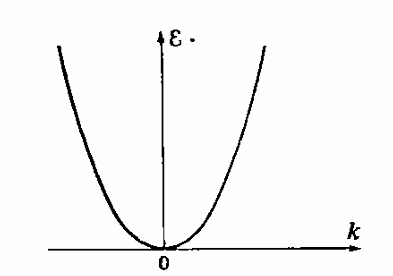
\includegraphics[width=0.4\textwidth]{images/4-Elettroni-Potenziale-Debole/livellien1Da.png}
	\caption{Livelli energetici di un elettrone libero (parabola).}
	\label{fig:livellien1Da}
\end{figure}

\textbf{(ii) Con Potenziale Periodico Debole:}  
La parabola dell'elettrone libero resta valida eccetto nelle vicinanze dei piani di Bragg.  
Quando \(q\) è vicino al piano di Bragg corrispondente a un vettore di reticolo \(K\), l'energia corretta si ottiene disegnando parabole centrate in \(K\).  
Questa rappresentazione è mostrata nella figura:
\begin{figure}[H]
	\centering
	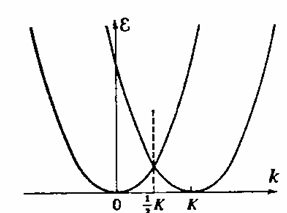
\includegraphics[width=0.4\textwidth]{images/4-Elettroni-Potenziale-Debole/livellien1Db.png}
	\caption{Livelli energetici in presenza di un potenziale periodico debole: parabole traslate.}
	\label{fig:livellien1Db}
\end{figure}

Al punto di intersezione delle parabole (piano di Bragg) la degenerazione viene risolta (split) di un ammontare pari a \(2|U_K|\) in modo che la derivata dell'energia sia nulla in quel punto. La figura successiva mostra la riproiezione con il gap:
\begin{figure}[H]
	\centering
	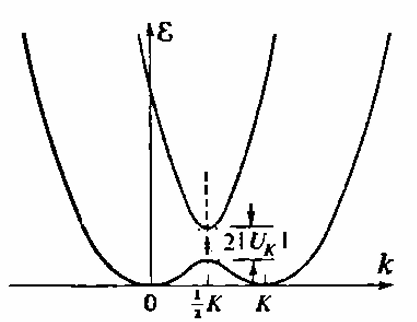
\includegraphics[width=0.4\textwidth]{images/4-Elettroni-Potenziale-Debole/livellien1Dc.png}
	\caption{Splitting delle parabole nelle vicinanze di un piano di Bragg.}
	\label{fig:livellien1Dc}
\end{figure}

La curva originale del caso libero (Figura~\ref{fig:livellien1Da}) si trasforma nella rappresentazione che si ottiene includendo l'effetto del potenziale (Figura~\ref{fig:livellien1Db}).  
Per visualizzare l'intera struttura a bande, si procede poi ad un'estensione nel cosiddetto \textbf{extended-zone scheme}, in cui ogni banda viene rappresentata nella propria zona di Brillouin:
\begin{figure}[H]
	\centering
	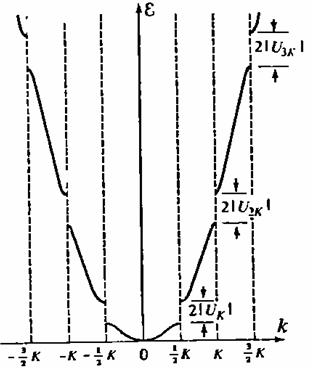
\includegraphics[width=0.4\textwidth]{images/4-Elettroni-Potenziale-Debole/livellien1De.png}
	\caption{Extended-zone scheme: ogni banda viene rappresentata nella corrispettiva zona di Brillouin.}
	\label{fig:livellien1De}
\end{figure}

Esistono schemi alternativi, come il \textbf{reduced zone scheme} (in cui tutte le bande vengono "riportate" nella prima zona di Brillouin) e il \textbf{repeated zone scheme}. Ad esempio, la figura seguente confronta i due schemi:
\begin{figure}[H]
	\centering
	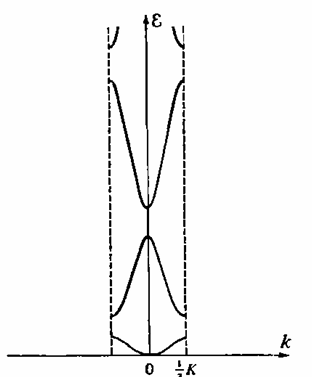
\includegraphics[width=0.4\textwidth]{images/4-Elettroni-Potenziale-Debole/reduced.png}
	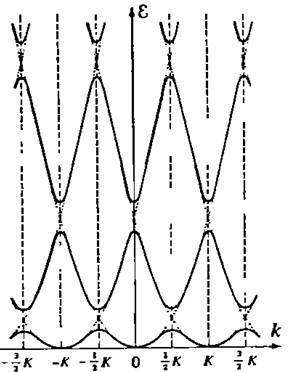
\includegraphics[width=0.4\textwidth]{images/4-Elettroni-Potenziale-Debole/repeated.png}
	\caption{A sinistra il reduced zone scheme, a destra il repeated zone scheme.}
	\label{fig:redrep}
\end{figure}

Infine, se il vettore di Fermi \(k_F\) si trova, ad esempio, tra \(-K\) e \(-\frac{1}{2}K\), dalla conoscenza di \(k_F\) è possibile dedurre immediatamente quante bande siano riempite.

\bigskip
\subsection{Bande Energetiche in Tre Dimensioni}
In tre dimensioni le bande energetiche, ottenute dalla soluzione dell'equazione agli autovalori per elettroni in un potenziale periodico, assumono forme complesse.  \\
Ad esempio, in un reticolo fcc privo di interazioni il grafico delle bande mostra punti di degenerazione in corrispondenza di punti specifici (ad es. il punto X) e il punto \(\Gamma\) rappresenta il centro della prima zona di Brillouin:
\begin{figure}[H]
	\centering
	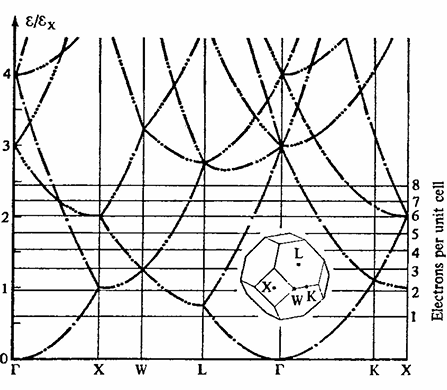
\includegraphics[width=0.6\textwidth]{images/4-Elettroni-Potenziale-Debole/bande3d1.png}
	\caption{Bande energetiche in 3D per un reticolo fcc senza interazioni.}
	\label{fig:bande3d1}
\end{figure}

Nel caso di materiali con interazioni (ad es. il silicio) la struttura a bande risulta modificata: in alcuni punti del reticolo reciproco (come X) possono rimanere degenerazioni mentre in altri (ad es. \(L\)) si apre un gap:
\begin{figure}[H]
	\centering
	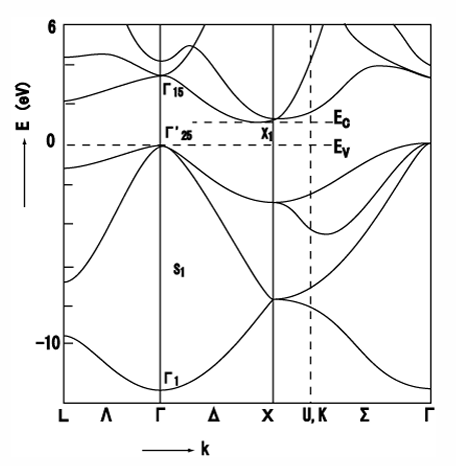
\includegraphics[width=0.6\textwidth]{images/4-Elettroni-Potenziale-Debole/bande3d2.png}
	\caption{Bande energetiche del silicio: si evidenziano gap e degenerazioni in diversi punti del reticolo reciproco.}
	\label{fig:bande3d2}
\end{figure}

\bigskip
\section{Zone di Brillouin}
Utilizzando la teoria degli elettroni in un potenziale, risulta possibile determinare l'intera struttura a bande tridimensionale di un cristallo.  
Si osserva che la posizione del vettore d'onda di Fermi fornisce informazioni sulle bande occupate:  
\begin{itemize}
	\item Se la superficie di Fermi imperturbata è completamente contenuta all'interno di una zona di Brillouin, allora la banda corrispondente è piena o parzialmente piena.
	\item Se invece la superficie di Fermi "spunta" da una zona di Brillouin (ovvero si trova tra due bande), la banda superiore risulterà vuota mentre quella inferiore sarà piena.
\end{itemize}
La figura seguente mostra le diverse zone di Brillouin per vari tipi di cristalli:
\begin{figure}[H]
	\centering
	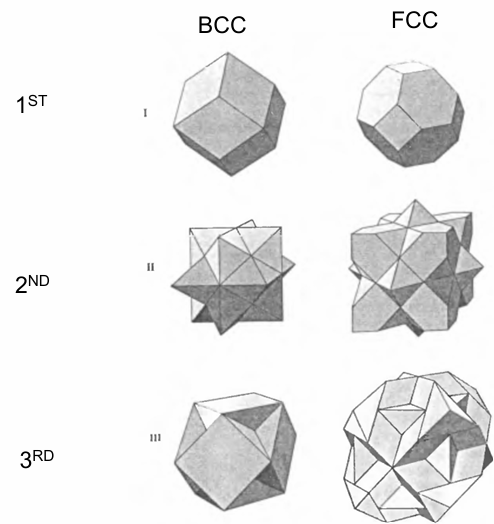
\includegraphics[width=0.6\textwidth]{images/4-Elettroni-Potenziale-Debole/zonediBr.png}
	\caption{Zone di Brillouin per diversi tipi di cristalli.}
	\label{fig:zonedibr}
\end{figure}


\bigskip
\section{Il Fattore di Struttura Geometrica in Reticoli con Base}
Quando il cristallo presenta più di un atomo per cella unitaria, il potenziale periodico derivante dagli ioni assume la forma
\[
U(\mathbf{r}) = \sum_{\mathbf{R}} \sum_j \phi\Bigl(\mathbf{r} - \mathbf{R} - \mathbf{d}_j\Bigr)\,,
\]
dove:
\begin{itemize}
	\item \(\mathbf{R}\) rappresenta il vettore di traslazione della cella unitaria,
	\item \(j\) scorre sugli atomi contenuti nella cella, che si trovano nelle posizioni \(\mathbf{d}_j\).
\end{itemize}
La componente Fourier del potenziale (cioè, la sua rappresentazione in \(\mathbf{K}\)-space) è definita da:
\[
U_{\mathbf{K}} = \frac{1}{v} \int_{\text{cella}} \d\mathbf{r}\, e^{-i\mathbf{K}\cdot\mathbf{r}}\, U(\mathbf{r})\,,
\]
dove \(v\) è il volume della cella unitaria.  
Inserendo l'espressione per \(U(\mathbf{r})\), si ha:
\[
U_{\mathbf{K}} = \frac{1}{v} \int_{\text{cella}} \d\mathbf{r}\, e^{-i\mathbf{K}\cdot\mathbf{r}} \sum_{\mathbf{R}} \sum_j \phi\Bigl(\mathbf{r} - \mathbf{R} - \mathbf{d}_j\Bigr)\,.
\]
Osserviamo che, poiché \(\phi(\mathbf{r})\) è un potenziale locale (importante solo in prossimità di ogni ione), la sommatoria sull'insieme delle traslazioni \(\mathbf{R}\) permette di estendere l'integrazione dalla cella unitaria a tutto lo spazio:
\[
U_{\mathbf{K}} = \frac{1}{v} \int_{\mathbb{R}^3} \d\mathbf{r}\, e^{-i\mathbf{K}\cdot\mathbf{r}} \sum_j \phi\Bigl(\mathbf{r} - \mathbf{d}_j\Bigr)\,.
\]
Definiamo quindi la trasformata di Fourier del potenziale locale:
\[
\phi(\mathbf{K}) = \int_{\mathbb{R}^3} \d\mathbf{r}\, e^{-i\mathbf{K}\cdot\mathbf{r}}\, \phi(\mathbf{r})\,,
\]
e il \emph{fattore di struttura}:
\[
S_{\mathbf{K}} = \sum_j e^{i\mathbf{K}\cdot\mathbf{d}_j}\,.
\]
Con queste definizioni la componente Fourier del potenziale risulta:
\[
U_{\mathbf{K}} = \frac{1}{v}\, \phi(\mathbf{K})\, S_{\mathbf{K}}^*\,.
\]
Riassumendo, il potenziale periodico in un reticolo con base si scrive come:
\[
\boxed{ U_{\mathbf{K}} = \frac{1}{v}\, \phi(\mathbf{K})\, S_{\mathbf{K}}^* \quad \text{con} \quad \phi(\mathbf{K}) = \int_{\mathbb{R}^3} \d\mathbf{r}\, e^{-i\mathbf{K}\cdot\mathbf{r}}\, \phi(\mathbf{r}), \quad S_{\mathbf{K}} = \sum_j e^{i\mathbf{K}\cdot\mathbf{d}_j}\,. }
\]
Questo risultato evidenzia che il potenziale Fourier \(U_{\mathbf{K}}\) è dato dal prodotto della forma del potenziale locale (tramite \(\phi(\mathbf{K})\)) e del fattore di struttura, che riflette la disposizione geometrica degli atomi nella cella unitaria.

\chapter{Dinamica Semiclassica degli Elettroni}

\section{Pacchetto d'onda di Bloch}
In un solido non tutti gli elettroni partecipano alla conduzione elettrica; infatti, sono principalmente quelli in prossimità del livello di Fermi a determinare le proprietà trasportistiche.\\
Considerando l'approccio classico di Sommerfeld, non è necessario localizzare l'elettrone su una scala comparabile alla distanza interatomica; pertanto, le equazioni di Newton possono essere applicate per descrivere la dinamica degli elettroni. In particolare, vale:
\[
\frac{\partial \vec{p}}{\partial t} = \hbar\, \frac{\partial \vec{k}}{\partial t} = \vec{F},
\]
dove \(\vec{k}\) è il vettore d'onda, \(\vec{p}=\hbar\vec{k}\) è l'impulso e \(\vec{F}\) è la forza esercitata sull'elettrone.\\
Tuttavia, poiché il valore di \(k_F\) è noto e tipicamente \(\Delta k\) è molto piccolo, il principio di indeterminazione
\[
\Delta k \, \Delta x \approx \hbar
\]
implica che l'incertezza nella posizione \(\Delta x\) risulti elevata. In altre parole, \textbf{per descrivere correttamente il sistema non si può considerare l'elettrone come una particella puntuale, ma bisogna ricorrere alla descrizione tramite un \emph{pacchetto d'onda}}. Nel nostro caso, adottiamo un'approssimazione semiclassica in cui il campo esterno non viene quantizzato.\\\\

Costruiamo dunque un pacchetto d'onda di Bloch centrato in \(\vec{r}_0\). Il pacchetto d'onda complessivo associato alla banda \(n\) si costruisce come una sovrapposizione ponderata di queste funzioni:
\[
\psi_n(\vec{r}) = \sum_k g(k)\psi_{n,k}(\vec{r})
\]
dove \(g(\vec{k})\) è una funzione peso scelta in modo da avere il pacchetto ben centrato in \(\vec{r}_0\). Se si scrive \(\vec{r} = \vec{r}_0 + \vec{R}\), con \(\vec{R}\) una coordinata relativa, il pacchetto risulta:
\[
\psi_n(\vec{r_0}+\vec{R}) = \sum_{k'} g(k')\psi_{n,k'}(\vec{r_0})e^{ik'R} = \sum_k \overline{g}(k')e^{ik'R}\]
 Tale espressione mostra che la funzione d'onda è delocalizzata rispetto alla posizione, estendendosi su più siti atomici. Il principio di indeterminazione
\[
\Delta k \, \Delta R \approx \hbar
\]
porta a
\[
\Delta R \approx \frac{\hbar}{\Delta k},
\]
quindi un piccolo intervallo in \(\vec{k}\) (intorno a \(k_F\)) implica un pacchetto d'onda molto esteso nello spazio reale.\\
\textbf{Questa delocalizzazione sottolinea che in un solido l'elettrone non è una particella localizzata, ma è rappresentato da un pacchetto d'onda composto da onde di Bloch aventi un vettore d'onda ben definito, che si estende su diverse celle primitive.}\\\\
La velocità di gruppo del pacchetto d'onda, che corrisponde alla velocità dell'elettrone, è data da:
\[
v_n(\vec{k}) = \frac{\partial \omega}{\partial \vec{k}} = \frac{1}{\hbar}\, \frac{\partial \varepsilon_n(\vec{k})}{\partial \vec{k}},
\]
con \(\varepsilon_n(\vec{k})\) l'energia della banda \(n\).

\subsection{Oscillazioni di Bloch}
Esaminiamo ora il comportamento degli elettroni sottoposti a un campo elettrico esterno. Se il potenziale elettrico è \(\phi\), il campo elettrico risulta:
\[
\vec{E} = - \vec{\nabla} \phi.
\]
Quando il campo agisce, l'energia totale di un elettrone nella banda \(n\) diventa:
\[
\varepsilon_n(\vec{k}(t)) - e\,\phi(\vec{r}(t)) = \text{costante}.
\]
Differenziando rispetto al tempo, si ottiene:
\[
\frac{d\varepsilon_n(\vec{k}(t))}{dt} - e\,\frac{d\phi(\vec{r}(t))}{dt} = 0.
\]
Utilizzando la relazione di catena per il tempo:
\[
\frac{d\varepsilon_n}{dt} = \frac{\partial \varepsilon_n}{\partial \vec{k}} \cdot \frac{\d\vec{k}}{dt} \quad \text{e} \quad \frac{d\phi}{dt} = \vec{\nabla} \phi \cdot \frac{d\vec{r}}{dt},
\]
e definendo la velocità di gruppo \(v_n(\vec{k}) = \frac{1}{\hbar} \frac{\partial \varepsilon_n}{\partial \vec{k}}\), si ottiene:
\[
\hbar\, \frac{\d\vec{k}}{dt} \cdot v_n(\vec{k}) - e\, \frac{d\vec{r}}{dt} \cdot \vec{\nabla} \phi = 0.
\]
Utilizzando il fatto che \(\frac{d\vec{r}}{dt}=v_n(\vec{k})\), la precedente uguaglianza diventa:
\[
v_n(\vec{k})\cdot\Bigl[\hbar\, \frac{\d\vec{k}}{dt} - e\,\nabla\phi\Bigr]=0.
\]
Dal momento che, in generale, \(v_n(\vec{k}) \neq 0\), si deve avere:
\[
\hbar\, \frac{\d\vec{k}}{dt} = e\,\nabla\phi = -e\,\vec{E}.
\]
Pertanto, l'evoluzione nel tempo del vettore d'onda risulta:
\begin{equation}
    \vec{k}(t) = \vec{k}_0 - \frac{e\, \vec{E}}{\hbar}\, t.
    \label{eqn:bloch_osc}
\end{equation}
Essendo l'energia periodica rispetto a \(\vec{k}\), ad esempio in una banda elettronica la funzione \(\varepsilon_n(\vec{k})\) possiede una periodicità determinata dalla zona di Brillouin; ciò significa che la velocità di gruppo
\[
v_n(\vec{k}(t)) = \frac{1}{\hbar}\, \frac{\partial \varepsilon_n(\vec{k}(t))}{\partial \vec{k}}
\]
risulterà anch'essa periodica. Di conseguenza, al variare del tempo, \textbf{la velocità può alternare segni positivi e negativi e l'elettrone oscillerà avanti e indietro: queste sono le oscillazioni di Bloch}. Un esempio schematico è riportato in Figura \ref{fig:OscillBloch}.
\begin{figure}[H]
	\centering
	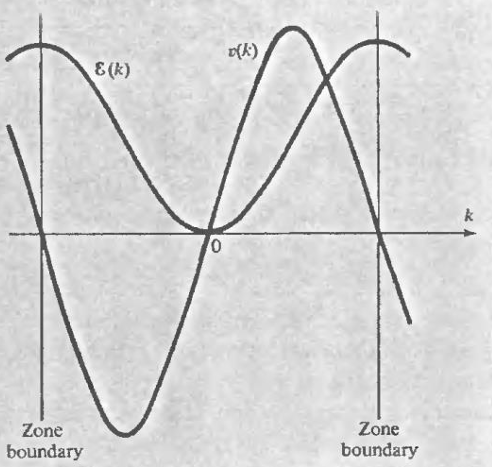
\includegraphics[width=0.4\textwidth]{images/5-Dinamica-Semiclassica/oscilldiBloch.png}
	\caption{Schema delle oscillazioni di Bloch. L'elettrone oscilla avanti e indietro nella banda, a causa della periodicità dell'energia in funzione del vettore d'onda.}
	\label{fig:OscillBloch}
\end{figure}

Nella maggior parte dei materiali reali il tempo d'oscillazione di Bloch è molto più lungo del tempo medio \(\tau\) tra gli scattering, così che questo effetto non è osservabile direttamente. Per evidenziarlo sarebbe necessario utilizzare campioni estremamente puri (con \(\tau\) elevato) oppure materiali in cui la zona di Brillouin sia molto piccola (cioè, con un intervallo \(\Delta k\) ridotto).

\section{Il Modello Semiclassico}
Le seguenti ipotesi semplificano la trattazione della dinamica degli elettroni in un solido:
\begin{enumerate}
    \item \textbf{Banda costante:} La banda \(n\) considerata resta la stessa in presenza del campo esterno; il campo è abbastanza debole da non indurre transizioni inter-banda. (In altre parole, il modello semiclassico non è in grado di descrivere processi di assorbimento che richiederebbero cambi di banda.)
    
    \item \textbf{Dinamica nel \(\vec{k}\)-spazio:} La dinamica del sistema è descritta dalle equazioni:
    \[
    \hbar \frac{\partial k}{\partial t} = e\vec{\nabla}\phi = -e\vec{E} \implies \vec{k}(t) = \vec{k}_0 - \frac{e\,\vec{E}}{\hbar}\, t.
    \]
    \[v_n(\vec{k}(t)) \equiv v\left(\vec{k}_0 -\frac{e\vec{E}}{\hbar}\cdot t \right)  = \frac{1}{\hbar} \frac{\partial \varepsilon_n(\vec{k}(t))}{\partial \vec{k}}\]
    
    \item \textbf{Vettore d'onda come numero quantico:} Il vettore \(\vec{k}\) caratterizza lo stato dell'elettrone, ma non coincide necessariamente con il classico concetto di momento. In un solido il vettore d'onda è definito dalla periodicità del reticolo ed è un numero quantico
    
    \item \textbf{Esclusione di Pauli:} Non è possibile che due elettroni occupino lo stesso stato quantico all'interno della stessa banda \(n\); ciò significa che non possono esistere due elettroni con la stessa posizione \(\vec{r}\) e con vettori d'onda differenti da un vettore reciproco \(\vec{K}\).
    
    \item \textbf{Distribuzione termica:} La distribuzione degli elettroni in funzione dell'energia è data dalla distribuzione di Fermi-Dirac:
    \[
    f\bigl(\varepsilon_n(\vec{k})\bigr)\, \frac{\d\vec{k}}{(2\pi)^3} = \frac{1}{e^{\beta\bigl(\varepsilon_n(\vec{k})-\mu\bigr)}+1}\, \frac{\d\vec{k}}{(2\pi)^3},
    \]
    dove \(\mu\) è il potenziale chimico e \(\beta = 1/(k_BT)\).
    \item \textbf{Perturbazione debole:} Il campo esterno è sufficientemente debole da soddisfare le seguenti condizioni:
    \begin{equation}
        \begin{split}
            eEa &\ll \frac{\bigl[\varepsilon_{\text{gap}}(\vec{k})\bigr]^2}{\varepsilon_F},\\[1mm]
            \hbar\omega_c &\ll \frac{\bigl[\varepsilon_{\text{gap}}(\vec{k})\bigr]^2}{\varepsilon_F},\\[1mm]
            \hbar\omega_c &\ll \varepsilon_{\text{gap}},\\[1mm]
            \lambda &\gg a,
        \end{split}
    \end{equation}
    dove \(a\) è la costante reticolare, \(\varepsilon_{\text{gap}}\) il gap energetico e \(\omega_c\) una frequenza caratteristica determinata dal campo.
\end{enumerate}


\subsection{Massa efficace}
Ora andiamo nel dettaglio della dinamica di un elettrone in un cristallo all'interno di una singola banda. Considero una funzione d'onda di Bloch $\psi_k(\mathbf{r}) = \frac{e^{i\mathbf{k}\cdot \mathbf{r}}}{\sqrt{V}}u_k(\mathbf{r})$ con $u_k(\mathbf{r}+\mathbf{R}) = u_k(\mathbf{r})$. \\
Data l'equazione di Schrodinger: 
\begin{equation}
    \begin{split}
        &H\psi = \varepsilon\psi \hspace{0.2cm}\text{divido da entrambe le parti:}\\
        &e^{-i \vec{k} \cdot \vec{r}}H e^{i \vec{k} \cdot \vec{r}}u_k(\vec{r}) = e^{-i \vec{k} \cdot \vec{r}}\varepsilon e^{+i \vec{k} \cdot \vec{r}}u_k(\vec{r})\\
        &H_k u_k(\vec{r}) = \varepsilon u_k(\vec{r}) \hspace{0.2cm}\text{autostato $u_k$ con stesso autovalore di H}\\
    \end{split}
\end{equation}
Per come si è definita $H_k$ possiamo riscriverla nel seguente modo:
\begin{equation}\label{eqn:Hk}
    \begin{split}
        &H_k \equiv e^{-i \vec{k} \cdot \vec{r}} H( \hat{\mathbf{p}}, \mathbf{r})  e^{i\vec{k} \cdot \vec{r}} = e^{-i\vec{k}\cdot \vec{r}} \left( -\frac{\hbar^2}{2m}\nabla^2+V \right) e^{i\vec{k}\cdot \vec{r}}\\
        &(-i\hbar \vec{\nabla}) e^{i\vec{k}\cdot\vec{r}}u_k(\vec{r}) = e^{i\vec{k}\cdot \vec{r}}(-i\hbar\vec{\nabla}+\hbar \vec{k})u_k(\vec{r}) \hspace{0.2cm}\text{da cui si ottiene:}\\
        &H_k\cdot u_k = e^{-i\vec{k}\cdot\vec{r}} \bigl[\frac{1}{2m}(-i\hbar\vec{\nabla}+\hbar \vec{k})^2+V\bigr]e^{i\vec{k}\cdot\vec{r}}\cdot u_k=\bigl[\frac{1}{2m}(-i\hbar\vec{\nabla}+\hbar \vec{k})^2+V\bigr]\cdot u_k\\
    \end{split}
\end{equation}
e quindi otteniamo:
\[ H( \hat{\mathbf{p}}, \mathbf{r}) \psi_k(\mathbf{r}) = \varepsilon_k\psi_k(\mathbf{r}) \implies H( \hat{\mathbf{p}} + \hbar \mathbf{k}, r) u_k(\mathbf{r}) = \varepsilon_k u_k(\mathbf{r})\]
Mostriamo che per il teorema di Herenfest la velocità è data da:
\[ v = \frac{d\mathbf{r}}{dt} = \frac{i}{\hbar}\left[ H, \mathbf{r}\right] \implies \braket{v_k^{(n)}} = \bra{\psi_k^{(n)}} \frac{d\mathbf{r}(t)}{dt} \ket{\psi_k^{(n)}} = \frac{i}{\hbar}\bra{\psi_k^{(n)}}\left[ H, \mathbf{r}\right]\ket{\psi_k^{(n)}} \]
Calcoliamo $\mathbf{\nabla}_kH_k$:
\begin{equation}
    \begin{split}
        &\mathbf{\nabla}_kH_k=\mathbf{\nabla}_k(e^{-i\vec{k}\cdot\vec{r}}\cdot H \cdot e^{i\vec{k}\cdot\vec{r}})=\\
        &=(-i\mathbf{r})e^{-i\vec{k}\cdot\vec{r}}He^{i\vec{k}\cdot\vec{r}} + e^{-i\vec{k}\cdot\vec{r}} \mathbf{\nabla}_k H e^{i\vec{k}\cdot\vec{r}} + e^{-i\vec{k}\cdot\vec{r}}H(i\mathbf{r})e^{i\vec{k}\cdot\vec{r}} \\
        &\text{il termine centrale si annulla in quanto non dipende da $k$}\\
        &=e^{-i\vec{k}\cdot\vec{r}}(-i\mathbf{r}H) e^{i\vec{k}\cdot\vec{r}} + e^{-i\vec{k}\cdot\vec{r}}(iH\mathbf{r}) e^{i\vec{k}\cdot\vec{r}}\\
        &=i(e^{-i\vec{k}\cdot\vec{r}}[H,\mathbf{r}]e^{i\vec{k}\cdot\vec{r}})\\
    \end{split}
\end{equation}
Da cui la velocità diventa:
\begin{equation}
    \begin{split}
        &\braket{v_k}= \bra{\psi_k} \frac{d\mathbf{r}(t)}{dt} \ket{\psi_k} = \frac{i}{\hbar}\bra{\psi_k}\left[ H, \mathbf{r}\right]\ket{\psi_k} \\
        & =\frac{i}{\hbar}\bra{u_k e^{-i\vec{k}\cdot\vec{r}}}\left[ H, \mathbf{r}\right]\ket{e^{i\vec{k}\cdot\vec{r}}u_k} = \frac{1}{\hbar} \bra{u_k}\mathbf{\nabla}_kH_k\ket{u_k} \hspace{0.2cm}\text{calcolando esplicitamente:}\\
        &=\frac{1}{\hbar} \bigl[\mathbf{\nabla_k} \bra{u_k} H_k \ket{u_k} -  \bra{\nabla_ku_k} H_k \ket{u_k} - \bra{u_k} H_k \ket{\nabla_k u_k}\bigr]\\
        &=\frac{1}{\hbar} \bigl[\mathbf{\nabla_k}\varepsilon(\mathbf{k}) -  \bra{\nabla_ku_k} H_k \ket{u_k} - \bra{u_k} H_k \ket{\nabla_k u_k}\bigr]\\
    \end{split}
\end{equation}
Osserviamo che siccome $\braket{u_k | u_k}=1$ la derivata è nulla per cui:
\begin{equation}
    \begin{split}
    &\bra{\nabla_ku_k} H_k \ket{u_k} = \varepsilon(\mathbf{k}) \braket{\nabla_k u_k | u_k}\\
    &\bra{u_k} H_k \ket{\nabla_k u_k} = \varepsilon(\mathbf{k}) \braket{u_k |\nabla_k u_k} \\
    & \vec{\nabla} \braket{u_k | u_k} = \braket{\vec{\nabla} u_k | u_k} + \braket{u_k | \vec{\nabla} u_k} = 0 \\
    & \implies \braket{\vec{\nabla} u_k | u_k} = - \braket{u_k | \vec{\nabla} u_k} 
    \end{split}
\end{equation}
Quindi il termine $-  \bra{\nabla_ku_k} H_k \ket{u_k} - \bra{u_k} H_k \ket{\nabla_k u_k}$ si elide e da qui si ottiene:
\begin{equation}
    \braket{v_k}= \frac{1}{\hbar} \mathbf{\nabla}_k\varepsilon(\mathbf{k})
\end{equation}
\\\\
Ora posso introdurre il concetto di \textbf{massa effettiva/efficace}, ossia a differenza del elettrone libero, la massa del elettrone non è quella classica ma è un tensore che dipende da k:
\begin{equation}
\begin{split}
    &\hbar \frac{d\mathbf{k}}{dt} = \mathbf{F} = m\mathbf{a}\\
    &\mathbf{a}=\frac{d\braket{v_k^{(n)}}}{dt} = \frac{d}{dt} \biggr(\frac{1}{\hbar}\mathbf{\nabla}_k\varepsilon(\mathbf{k}(t)\biggr)\\
    &=\frac{1}{\hbar}\left( \frac{dk}{dt} \frac{\partial}{\partial k_j} \right) \frac{\partial}{\partial k_i}\varepsilon_k^{(n)} \\
    &= \left( \hbar \frac{dk_j}{dt}\right)\left[ \frac{1}{\hbar^2} \frac{\partial^2 \varepsilon_k^{(n)}}{\partial k_j \partial k_i}\right]= \frac{\mathbf{F}}{m} = \left( \hbar \frac{dk_j}{dt}\right) \frac{1}{\overline{m}_{ij}^{(n)}(k)}
\end{split}
\end{equation} 
Il parametro di proporzionalità tra la forza e la accelerazione non è più uno scalare ma il tensore di massa efficace:
\begin{equation}
    m_{ij} = \left( \frac{1}{\hbar^2} \frac{\partial^2 \varepsilon_k}{\partial k_j \partial k_i}\right)^{-1}
\end{equation}
La massa efficace tiene conto degli effetti che agiscono sugli elettroni quando si muovono all'interno di un reticolo periodico, può essere positiva o negativa a seconda del valore di $\mathbf{k}$ ma questo dipende anche dal tipo di banda, nella banda di conduzione la massa efficace è positiva (elettroni) mentre in quella di valenza è negativa (lacune). Per avere un elettrone molto pesante mi serve una banda molto piatta ($\partial^2\varepsilon$ piccola), solitamente negli isolanti le bande sono piatte (elettroni più "pesanti) ed è per questo che gli elettroni si muovono molto lentamente. 

\section{Probabilità di Scattering}
Consideriamo un sistema in cui avviene lo scattering elastico degli elettroni. Le ipotesi principali sono:
\begin{enumerate}
    \item Lo scattering è elastico, cioè l'energia dell'elettrone rimane invariata.
    \item La probabilità di transizione \(W_{k,k'}\) dall'onda piana di vettore d'onda \(\vec{k}\) a quella di vettore \(\vec{k}'\) è indipendente dalla distribuzione elettronica.
    \item È simmetrica, ovvero \(W_{k,k'} = W_{k',k}\).
    \item Si può utilizzare la regola d'oro di Fermi per calcolare la probabilità di transizione, dato che l'urto provoca una transizione tra stati quantistici.
\end{enumerate}
La probabilità che un elettrone nello stato \(\vec{k}\) venga scatterato, in un intervallo di tempo infinitesimale \(dt\), in un qualsiasi stato nell'elemento di volume \(\d\vec{k}'\) è data da:
\[
\frac{W_{k,k'}\,\d{t}\,\d\vec{k}'}{(2\pi)^3}.
\]
In particolare, utilizzando la regola d'oro di Fermi, il tasso di transizione è:
\[
W_{k,k'} = \frac{2\pi}{\hbar}\, n_i\, \delta\Bigl(\varepsilon(\vec{k})-\varepsilon(\vec{k}')\Bigr)\, \bigl|\langle \vec{k}|U|\vec{k}'\rangle \bigr|^2,
\]
dove:
\begin{itemize}
    \item \(n_i\) è il numero di impurità (o la densità delle stesse) che generano la perturbazione,
    \item \(U\) è il potenziale introdotto dalle impurità, che rompe la periodicità del potenziale cristallino,
    \item La \(\delta\)-di Dirac impone la conservazione dell'energia (scattering elastico).
\end{itemize}
La probabilità totale di scattering per unità di tempo per uno stato \(\vec{k}\) si ottiene integrando su tutti gli stati finali disponibili:
\[
\frac{1}{\tau(\vec{k})} = \int \frac{\d\vec{k}'}{(2\pi)^3}\, W_{k,k'}\,[1-f(\vec{k}')],
\]
dove \(f(\vec{k}')\) è la funzione di distribuzione degli elettroni negli stati finali e il termine \([1-f(\vec{k}')]\) rappresenta la probabilità che lo stato \(\vec{k}'\) sia vuoto (il principio di esclusione di Pauli).\\\\
Per descrivere il processo di scattering nel sistema, si schematizza il flusso in uscita ed in ingresso in un dato stato \(\vec{k}\):

\subsubsection*{Flusso in Uscita}
La probabilità che un elettrone in uno stato \(\vec{k}\) venga scatterato fuori da questo stato (ossia, perda la propria occupazione) è data da:
\[
\left(\frac{df(\vec{k})}{dt}\right)_{\text{out}} = -\frac{f(\vec{k})}{\tau(\vec{k})} = - f(\vec{k}) \int \frac{\d\vec{k}'}{(2\pi)^3}\, W_{k,k'}\,[1-f(\vec{k}')].
\]

\subsubsection*{Flusso in Ingresso}
Analogamente, la probabilità che uno stato \(\vec{k}\) venga occupato da un elettrone proveniente da un altro stato \(\vec{k}'\) è:
\[
\left(\frac{df(\vec{k})}{dt}\right)_{\text{in}} = [1-f(\vec{k})] \int \frac{\d\vec{k}'}{(2\pi)^3}\, W_{k',k}\, f(\vec{k}'),
\]
dove \([1-f(\vec{k})]\) è la probabilità che lo stato \(\vec{k}\) sia vuoto e \(f(\vec{k}')\) è la probabilità che lo stato \(\vec{k}'\) sia occupato.

\subsubsection*{Termine Collisionale}
Combinando i contributi in uscita e in ingresso, il termine collisionale totale diventa:
\begin{equation}\label{eqn:coll}
\begin{split}
\left(\frac{df(\vec{k})}{dt}\right)_{\text{coll}} &= \left(\frac{df(\vec{k})}{dt}\right)_{\text{in}} + \left(\frac{df(\vec{k})}{dt}\right)_{\text{out}} \\
&= [1-f(\vec{k})] \int \frac{\d\vec{k}'}{(2\pi)^3}\, W_{k',k}\, f(\vec{k}') - f(\vec{k}) \int \frac{\d\vec{k}'}{(2\pi)^3}\, W_{k,k'}\,[1-f(\vec{k}')].
\end{split}
\end{equation}
Utilizzando la simmetria \(W_{k,k'} = W_{k',k}\) e riorganizzando i termini, si trova che:
\[
\left(\frac{df(\vec{k})}{dt}\right)_{\text{coll}} = - \int \frac{\d\vec{k}'}{(2\pi)^3}\, W_{k,k'}\,[f(\vec{k}) - f(\vec{k}')].
\]

\subsection{Relaxation Time Approximation}
Per semplificare ulteriormente il problema, si introduce l'approssimazione del tempo di rilassamento. Questa approssimazione si basa su due ipotesi:
\begin{enumerate}
    \item Il tempo medio di collisione \(\tau(\vec{k})\) non dipende dalla funzione di distribuzione stessa $f$, e si assume identico per le collisioni in uscita e in ingresso; in altre parole, la probabilità di transizione da \(\vec{k}\) a \(\vec{k}'\) è simmetrica e può essere caratterizzata da un unico \(\tau(\vec{k})\).
    \item Dopo un tempo sufficientemente lungo, il sistema si porta in equilibrio e la distribuzione degli elettroni assume la forma di \(f_0(\vec{k})\), la distribuzione di Fermi-Dirac locale.
\end{enumerate}
Sostituendo \(f(\vec{k}') \to f_0(\vec{k}')\) nella Eq. \eqref{eqn:coll} e considerando che il sistema tende a portarsi verso l'equilibrio, si definisce il termine collisionale nella \emph{relaxation time approximation} come:
\[
\left(\frac{df(\vec{k})}{dt}\right)_{\text{coll}} = -\frac{f(\vec{k})-f_0(\vec{k})}{\tau(\vec{k})}.
\]

\subsubsection*{Equazione Cinematica (Teorema di Liouville)}
Un altro importante concetto è che, in assenza di collisioni, il teorema di Liouville stabilisce che il volume in spazio delle fasi è conservato. In presenza di scattering, questa condizione non risulta più valida e lo stato della funzione di distribuzione varia secondo:
\begin{equation}\label{eqn:liouville}
f(\vec{k},\vec{r}, t) \to f(\vec{k}+\d\vec{k},\, \vec{r}+d\vec{r},\, t+dt) = f(\vec{k},\vec{r},t) + \left[\frac{\partial f}{\partial t}\right]_{\text{coll}} dt.
\end{equation}
D'altro canto, se consideriamo il movimento degli elettroni in modo semiclassico, un elettrone sottoposto a una forza \(\vec{F}\) subirà una variazione del vettore d'onda data da:
\[
\d\vec{k} = \frac{\vec{F}}{\hbar}\, dt,
\]
e la posizione cambierà di:
\[
d\vec{r} = \vec{v}\, dt,
\]
con \(\vec{v}\) la velocità del pacchetto d'onda. Pertanto, espandendo in serie di Taylor, si ha:
\begin{equation}
\begin{split}
f\Bigl(\vec{k}+\frac{\vec{F}}{\hbar}\,dt,\, \vec{r}+\vec{v}\,dt,\, t+dt\Bigr) &\approx f(\vec{k},\vec{r},t) + \frac{\partial f}{\partial \vec{r}}\cdot \vec{v}\,dt \\
&\quad + \frac{\partial f}{\partial \vec{k}}\cdot \frac{\vec{F}}{\hbar}\, dt + \frac{\partial f}{\partial t}\, dt.
\end{split}
\end{equation}
Equagliando questa espansione con l'evoluzione data da \eqref{eqn:liouville}, si ottiene:
\begin{equation}\label{eqn:boltzmann}
\frac{\partial f}{\partial t} + \vec{v}\cdot \frac{\partial f}{\partial{\vec{r}}}  + \frac{\vec{F}}{\hbar}\cdot  \frac{\partial f}{\partial{\vec{k}}} = -\frac{f - f_0}{\tau},
\end{equation}
che è la forma semplificata dell'equazione di Boltzmann in presenza di collisioni, nella \emph{relaxation time approximation}.

\subsubsection*{Soluzione Semplice in Assenza di Gradiente Spaziale}

Se supponiamo che inizialmente al tempo \(t=0\) il sistema sia disturbato e che la forza esterna sia nulla (ovvero nessun gradiente spaziale) oppure il sistema è isotropo (cosicché \(\nabla_{\vec{r}} f = 0\)), l'equazione \eqref{eqn:boltzmann} si riduce a:
\[
\frac{\partial f}{\partial t} = -\frac{f-f_0}{\tau}.
\]
La cui soluzione è immediata e prende la forma:
\[
f(\vec{k},t) = f_0(\vec{k}) + \left[f(\vec{k},0)-f_0(\vec{k})\right] e^{-t/\tau}.
\]
Questa soluzione mostra che la funzione di distribuzione \(f\) si rilassa esponenzialmente verso la distribuzione di equilibrio \(f_0\) con un tempo caratteristico \(\tau\).

\bigskip
\noindent \textbf{Nota:} Il meccanismo di scattering (spesso dovuto alle impurità) che impedisce l'osservazione completa delle oscillazioni di Bloch è anche la causa della resistività nei materiali. Inoltre, si assume che gli elettroni interagiscano debolmente tra loro, poiché il contributo medio delle interazioni elettrone-elettrone si annulla in un sistema omogeneo (la "nuvola elettronica" appare quasi simmetrica).

\section{Trattazione Semiclassica del Risultato di Drude}
Il modello di Drude descrive la conduzione elettrica in un metallo attraverso la relazione
\[
\vec{J} = \sigma\, \vec{E} \quad \text{con} \quad \sigma = \frac{n\,e^2\,\tau}{m},
\]
dove \(n\) è la densità totale degli elettroni, \(e\) la carica elementare, \(\tau\) il tempo medio di collisione (o tempo di rilassamento) e \(m\) la massa dell'elettrone.\\\\
Nell'approccio semiclassico considerato, si assume che solo gli elettroni in prossimità del livello di Fermi partecipino alla conduzione. In presenza di una perturbazione esterna, la sfera di Fermi in \(\vec{k}\)-spazio inizia a spostarsi e avvengono collisioni (scattering). Gli elettroni, passando in stati vuoti di energia inferiore, subiscono scattering che in media comporta una piccola traslazione della sfera di Fermi, la quale risulta responsabile del flusso di corrente.\\\\
La densità di corrente totale si scrive come
\begin{equation}
    \vec{J} = 2 \int \frac{\d\vec{k}}{(2\pi)^3}\, (-e)\,\vec{v}(\vec{k})\, f(\vec{k}),
\end{equation}
dove il fattore 2 tiene conto della degenerazione per spin, \(\vec{v}(\vec{k})\) è la velocità di gruppo associata a uno stato con vettore d'onda \(\vec{k}\) e \(f(\vec{k})\) è la funzione di distribuzione degli elettroni.\\\\
Si assume che, in presenza di una perturbazione debole, la funzione di distribuzione possa essere scritta come
\[
f(\vec{k}) = f_0(\vec{k}) + f_1(\vec{k}),
\]
dove \(f_0(\vec{k})\) è la distribuzione di equilibrio (la distribuzione di Fermi–Dirac) e \(f_1(\vec{k})\) una piccola variazione dovuta al campo esterno\\
Utilizzando l'approssimazione del tempo di rilassamento, dall'equazione del termine collisionale (vedi la trattazione precedente) in un sistam isotropo e indipendente dal tempo si ottiene:
\[
\frac{1}{\hbar}\,\frac{\partial f_0}{\partial \vec{k}} \cdot \vec{F} = \frac{1}{\hbar}\,\frac{\partial f_0}{\partial \vec{k}} \cdot (-e\,\vec{E}) = -\frac{f(\vec{k})-f_0(\vec{k})}{\tau},
\]
da cui si ricava
\[
f(\vec{k}) = f_0(\vec{k}) + \frac{e\,\tau}{\hbar}\,\frac{\partial f_0}{\partial \vec{k}} \cdot \vec{E} \equiv f_0(\vec{k}) + f_1(\vec{k}) f(\mathbf{k}) \approx f_0(\mathbf{k}+\frac{e\tau}{\hbar}\mathbf{E})\]
per una perturbazione $e\tau \mathbf{E}<<\hbar \mathbf{k}_f$\\
Un'altra forma equivalente, esprimendo la derivata rispetto a \(\vec{k}\) in funzione della derivata rispetto all'energia \(\varepsilon\), è
\[
f_1(\vec{k}) = \frac{e\,\tau}{\hbar}\,\frac{\partial f_0}{\partial \varepsilon}\,\frac{\partial \varepsilon}{\partial \vec{k}} \cdot \vec{E} = e\,\tau\,\frac{\partial f_0}{\partial \varepsilon}\,\vec{v}(\vec{k}) \cdot \vec{E}.
\]
Inserendo questa correzione nella definizione della corrente, la densità di corrente diventa
\[
\vec{J} = \frac{-2e}{(2\pi)^3} \int \d\vec{k}\, \vec{v}(\vec{k})\, \left[f_0(\vec{k}) + f_1(\vec{k})\right].
\]
Il contributo dovuto a \(f_0\) si annulla per simmetria (la sfera di Fermi è isotropa in assenza di campo), perciò rimane
\[
\vec{J} = \frac{-2e}{(2\pi)^3} \int \d\vec{k}\, \vec{v}(\vec{k})\, f_1(\vec{k}).
\]
Sostituendo \(f_1(\vec{k})\) si ottiene
\[
\vec{J} = \frac{-2e}{(2\pi)^3} \int \d\vec{k}\, \vec{v}(\vec{k})\, \left[ e\,\tau\,\frac{\partial f_0}{\partial \varepsilon}\,\vec{v}(\vec{k}) \cdot \vec{E}\right].
\]
Possiamo esprimere questo risultato componente per componente come:
\[
J_\alpha = \frac{e^2}{4\pi^3} \int \d\vec{k}\, \tau\, \left(-\frac{\partial f_0}{\partial \varepsilon}\right)\, v_\alpha(\vec{k})\,\left[\vec{v}(\vec{k}) \cdot \vec{E}\right].
\]
Definendo il tensore di conducibilità mediante \(J_\alpha = \sum_\beta \sigma_{\alpha\beta}\, E_\beta\) e, in un sistema isotropo, scegliendo la direzione del campo \(\vec{E}\) lungo il versore \(\hat{e} = \frac{\vec{E}}{|\vec{E}|}\), si ha
\[
\sigma_0 = \frac{e^2}{4\pi^3} \int \d\vec{k}\, \tau\, \left(-\frac{\partial f_0}{\partial \varepsilon}\right) \, (\hat{e} \cdot \vec{v}(\vec{k}))^2.
\]
In un sistema isotropo la media vale
\[
v_x^2+v_y^2+v_z^2 = v \implies v_x^2 = \frac{v^2}{3} \implies (\hat{e} \cdot \vec{v}(\vec{k}))^2 = \frac{v^2(\vec{k})}{3}.
\]
Inoltre, a basse temperature, la derivata \(-\frac{\partial f_0}{\partial \varepsilon}\) è fortemente concentrata attorno all'energia di Fermi e può essere approssimata con una \(\delta\)-di Dirac:
\[
-\frac{\partial f_0}{\partial \varepsilon} = \delta\bigl(\varepsilon(\vec{k})-\varepsilon_F\bigr).
\]
Utilizzando la definizione della densità degli stati per la banda \(n\)
\[
g_n(\varepsilon) = \frac{1}{(2\pi)^3}\int \delta\bigl(\varepsilon_n(\vec{k})-\varepsilon\bigr)\, \d\vec{k} = \frac{1}{(2\pi)^3} \int_{S_\varepsilon} \frac{\d{S}}{|\nabla_{\vec{k}} \varepsilon(\vec{k})|},
\]
si giunge a
\[
\sigma_0 = \frac{e^2}{3\cdot 4\pi^3} \int \d\vec{k}\, \tau\, v^2(\vec{k})\, \delta\bigl(\varepsilon(\vec{k})-\varepsilon_F\bigr)
= \frac{e^2}{12 \pi^3}\, \tau_F\, v_F^2 \int_{S_F} \frac{\d{S}}{|\vec{\nabla} \varepsilon(\vec{k})|},
\]
dove \(S_F\) è la superficie di Fermi, mentre \(\tau_F\) e \(v_F\) rappresentano il tempo di rilassamento e la velocità a \(k_F\).\\

ricordando che valgono le seguenti relazioni 
\[
 k_F^3 = 3\pi^2\, n \quad v_F = \frac{\hbar k_F}{\overline{m}} \quad \vec{v} = \frac{1}{\hbar}\cdot\nabla\varepsilon(\vec{k}) 
\]
si ottiene la classica formula di Drude:
\[
\sigma_0 = \frac{e^2\,\tau_F}{m^*}\, n.
\]
\vspace{1em}
\section{Lacune}
La conduzione in un metallo è dovuta esclusivamente agli elettroni presenti in bande parzialmente piene. Infatti, le bande completamente piene sono sempre all'equilibrio poiché, nell'approccio semiclassico, il teorema di Liouville garantisce la conservazione del volume nello spazio delle fasi (cioè, la conservazione contemporanea della posizione e del vettore d'onda). Di conseguenza, anche in presenza di campi elettrici e magnetici dipendenti da posizione e tempo, una banda completamente piena resta tale, in quanto le modifiche di stato causate dalla perturbazione si bilanciano esattamente.\\\\
Possiamo infatti esprimere la densità di corrente \(\vec{J}\) come
\begin{equation}
    \vec{J} = (-e) \int \frac{\d\vec{k}}{(4\pi^3)} \, \frac{1}{\hbar}\frac{\partial \varepsilon(\vec{k})}{\partial \vec{k}},
\end{equation}
e l'energia totale come
\begin{equation}
    U = \int \frac{\d\vec{k}}{(4\pi^3)} \, \varepsilon(\vec{k}) \,\frac{1}{\hbar}\frac{\partial \varepsilon(\vec{k})}{\partial \vec{k}}.
\end{equation}
Se l'integrale si estende su tutta la zona di Brillouin e la funzione \(\varepsilon(\vec{k})\) riguarda una banda completamente piena, i contributi relativi alle velocità con segni positivi e negativi si cancellano (perché la funzione è periodica e simmetrica), e quindi entrambi gli integrali risultano nulli. Questo implica che le bande piene non contribuiscono alla conduzione elettrica.\\\\
La conduzione è dunque determinata esclusivamente dalle "quasi particelle" presenti in bande parzialmente piene, dove esistono degli stati vuoti (dette anche \emph{lacune}) in cui gli elettroni possono muoversi.

\subsection*{Concetto di Lacuna}

Il termine \emph{lacuna} indica uno stato non occupato in una banda che, altrimenti, sarebbe completamente piena. Le lacune non sono particelle elementari, ma quasiparticelle che nascono dall'azione collettiva degli elettroni. Consideriamo i seguenti punti:
\begin{itemize}
    \item Quando la banda è completamente piena, la somma vettoriale dei vettori d'onda degli elettroni è uguale a zero: \(\sum_i \vec{k}_i = 0\).
    \item Se si rimuove un elettrone dalla banda (ad es. un elettrone con vettore d'onda \(\vec{k}_e\) viene promosso in una banda di conduzione), la somma dei vettori d'onda degli elettroni rimasti diventa
    \[
    \sum_i \vec{k}_i = -\vec{k}_e,
    \]
    e dunque, per mantenere la condizione di equilibrio (la somma totale deve restare zero), il vettore d'onda associato allo stato vuoto (la lacuna) deve essere:
    \[
    \vec{k}_h = -\vec{k}_e.
    \]
\end{itemize}
Questo procedimento è una conseguenza del fatto che, essendo un effetto collettivo, la definizione della lacuna nasce dalla differenza fra l'insieme degli stati occupati e la condizione di band complete. In altre parole, se scriviamo:
\[
\sum_i \vec{k}_i = \sum_{\text{occupati}} \vec{k}_i + \sum_{\text{non occupati}} \vec{k}_i = 0,
\]
allora la mancanza di un elettrone in un particolare stato si traduce in un contributo netto uguale al vettore \(-\vec{k}_e\).

\subsection*{Energia della Lacuna}
Per quanto riguarda l'energia, immaginiamo di avere una banda di valenza completamente piena e una banda di conduzione completamente vuota, come illustrato in Figura~\ref{fig:lacune1}. Se, promuovendo un elettrone dallo stato \(\vec{k}_e\) della banda di valenza (VB) a uno stato della banda di conduzione (CB) mediante l'assorbimento di un fotone (con \(\hbar\omega > E_g\), dove \(E_g\) è il gap energetico), si crea nello stesso momento una lacuna nella banda di valenza, la reazione è:
\[
e(\text{VB}) + \text{fotone}\, (\hbar\omega > E_g) \to e(\text{CB}) + h(\text{VB}).
\]
Quando la banda di valenza è piena, la somma totale dei vettori d'onda è nulla:
\[
\vec{k}_{\text{band}} = \sum_i \vec{k}_i = 0.
\]
Pertanto, rimuovendo un elettrone con vettore \(\vec{k}_e\) si ottiene che il vettore d'onda della lacuna è:
\[
\vec{k}_h = -\vec{k}_e.
\]
Per quanto riguarda l'energia, convenzionalmente si prende $E_e(\text{VB}) < 0$,
\[ E_e(\text{VB}) + \hbar\omega = E_e(\text{CB})\]
Ma
\[\hbar\omega = E_e(\text{CB}) + E_h(\text{VB}) \]
Da cui si ricava 
\[E_e(\text{VB})+ \cancel{E_e(\text{CB})} + E_h(\text{VB}) = \cancel{E_e(\text{CB})}
    \implies E_h(\text{VB}) = - E_e (\text{VB})\]
Questo risultato esprime il fatto che, dal punto di vista delle lacune, lo spazio e l'energia si conservano: per ridurre l'energia, l'elettrone in banda di conduzione tenderà a scendere (per minimizzare l'energia totale) mentre la lacuna, per effetto opposto, tenderà a spostarsi verso energie più elevate nella banda di valenza.


\subsection*{Massa Efficace e Velocità della Lacuna}
La massa efficace della lacuna si ricava dalla seconda derivata dell'energia rispetto al vettore d'onda. Formalmente, si scrive:
\[
\frac{1}{m_h^*} = \frac{1}{\hbar^2} \frac{\partial^2 E_h(\vec{k}_h)}{\partial k_i^{(h)} \partial k_j^{(h)}}.
\]
Utilizzando la relazione \(E_h(\vec{k}_h) = -E_e(\vec{k}_e)\) e \(\vec{k}_h = - \vec{k}_e\), si ottiene:
\[
\frac{1}{m_h^*} = -\frac{1}{\hbar^2} \frac{\partial^2 E_e(\vec{k}_e)}{\partial k_i^{(e)} \partial k_j^{(e)}}.
\]
Quindi, la massa efficace della lacuna risulta essere:
\[
m_h^* = - m_e^*.
\]
Analogamente, la velocità di gruppo della lacuna è definita come
\[
v_h(\vec{k}_h) = \frac{1}{\hbar} \frac{\partial E_h(\vec{k}_h)}{\partial \vec{k}_h}.
\]
Utilizzando la relazione \(E_h(\vec{k}_h) = -E_e(\vec{k}_e)\) e \(\vec{k}_h = -\vec{k}_e\), si trova:
\[
v_h(\vec{k}_h) = \frac{1}{\hbar} \frac{\partial E_e(\vec{k}_e)}{\partial \vec{k}_e} = v_e(\vec{k}_e).
\]
Pertanto, la velocità della lacuna coincide con quella dell'elettrone, mentre la massa efficace ha il segno opposto.

\subsection*{Comportamento in Presenza di una Forza Esterna}

Consideriamo l'effetto di una forza esterna sul sistema. Dal punto di vista della lacuna, l'evoluzione del vettore d'onda è governata da
\[
\hbar \frac{\d\vec{k}_h}{dt} = q_h \left[\vec{E} + \vec{v}_h \times \vec{B}\right],
\]
mentre dal punto di vista dell'elettrone:
\[
\hbar \frac{d\vec{k}_e}{dt} = q_e \left[\vec{E} + \vec{v}_e \times \vec{B}\right],
\]
dove \(q_e = -e\). Poiché \(\vec{k}_h = -\vec{k}_e\), derivando rispetto al tempo si ottiene:
\[
- \hbar \frac{d\vec{k}_e}{dt} = q_h \left[\vec{E} + \vec{v}_e \times \vec{B}\right].
\]
La relazione per l'elettrone è:
\[
\hbar \frac{d\vec{k}_e}{dt} = -e \left[\vec{E} + \vec{v}_e \times \vec{B}\right].
\]
Le due equazioni saranno compatibili se:
\[
q_h = -q_e = +e.
\]
Questo conferma che, dal punto di vista dinamico, la lacuna si comporta come una particella con carica positiva \(+e\).

\subsection*{Conclusioni sul Ruolo delle Lacune}
La conduzione elettrica è determinata dal riempimento delle bande:
\begin{enumerate}
    \item \textbf{Metalli:} Presentano almeno una banda parzialmente piena, in cui la conduzione è dovuta principalmente agli elettroni.
    \item \textbf{Semimetalli:} Hanno il livello di Fermi posizionato in una regione con densità di stati molto bassa, e quindi pochi portatori contribuiscono al trasporto.
    \item \textbf{Semiconduttori:} La banda di valenza è quasi piena e la banda di conduzione quasi vuota; la conduzione avviene promuovendo elettroni dalla banda di valenza alla banda di conduzione, generando contemporaneamente lacune.
    \item \textbf{Isolanti:} Presentano una banda di valenza completamente piena e una banda di conduzione vuota, separati da un gap energetico elevato, rendendo difficile l'eccitazione di elettroni.
\end{enumerate}
Possiamo vedere anche il comportamento della densità di corrente integrando sull'intera zona di Brillouin:
\[
j = \int_{\text{BZ}} \frac{\d\vec{k}}{(4\pi^3)}\, (-e)\, v(\vec{k}) = 0,
\]
perché, in una banda completamente piena, le componenti della corrente dovute agli stati occupati si annullano per simmetria. Possiamo scrivere questo risultato come:
\[
0 = \int_{\text{occupati}} \frac{\d\vec{k}}{(4\pi^3)}\, (-e)\, v(\vec{k}) + \int_{\text{non occupati}} \frac{\d\vec{k}}{(4\pi^3)}\, (-e)\, v(\vec{k}).
\]
Da qui si può ricavare che:
\[
\int_{\text{non occupati}} \frac{\d\vec{k}}{(4\pi^3)}\, (-e)\, v(\vec{k}) = \int_{\text{occupati}} \frac{\d\vec{k}}{(4\pi^3)}\, (+e)\, v(\vec{k}),
\]
il che significa che la corrente prodotta se si trascurano gli elettroni negli stati occupati è equivalente a quella prodotta dalle lacune, che agiscono come portatori con carica \(+e\).





\chapter{Misurazione della Superficie di Fermi}

Ci sono diversi effetti sperimentali che permettono di misurare la superficie di Fermi; una volta nota la sua forma, è possibile ricavare informazioni approfondite sulla struttura delle bande elettroniche nel solido.

\section{De Haas--van Alphen Effect}

L'effetto De Haas--van Alphen consiste nella misurazione della magnetizzazione \(M\) di un campione (ad esempio, di Bismuto) in funzione del campo magnetico \(H\) a temperature molto basse (ad esempio, \SI{14.2}{\kelvin}).  \\
In tali esperimenti si osservano oscillazioni del rapporto \(M/H\) nonché oscillazioni analoghe nelle grandezze come la suscettività magnetica, la conduttività e la magnetoresistenza, quando queste vengono tracciate in funzione dell'inverso del campo magnetico, \(1/H\).\\\\

Landau aveva già mostrato che l'oscillazione di un elettrone libero in campo magnetico deriva dalla quantizzazione delle orbite elettroniche.  
Successivamente, Osanger introdusse quella che viene chiamata la \textbf{legge di Osanger}, secondo la quale il cambiamento nell'inverso del campo magnetico in un singolo periodo d'oscillazione è dato da:
\[
\Delta\left(\frac{1}{H}\right) = \frac{2\pi e}{\hbar c}\,\frac{1}{A_e}\,,
\]
dove \(A_e\) \textbf{rappresenta l'area della sezione trasversale della superficie di Fermi}, calcolata lungo la direzione normale al campo magnetico.  
\textbf{Variando il campo magnetico, dunque, si possono attraversare sezioni diverse della superficie di Fermi e, in questo modo, si può “mappare” l'intera superficie.}  \\
Si ricorda che gli elettroni coinvolti sono quelli prossimi all'energia di Fermi, poiché solo loro partecipano attivamente alla conduzione.

\begin{figure}[H]
	\centering
	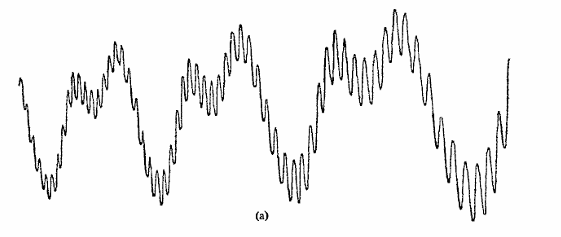
\includegraphics[width=0.8\textwidth]{images/6-Superficie-Fermi/vanalphen.png}
	\caption{Esempio di oscillazioni dell'effetto De Haas--van Alphen nel Renio.}
	\label{fig:vanalphen}
\end{figure}


\subsection{Origine del Fenomeno Oscillatorio}
Per comprendere a fondo il comportamento oscillatorio delle varie grandezze al variare del campo magnetico, è necessario analizzare come la presenza del campo alteri la densità degli stati elettronici.

\subsubsection{Livelli di Landau}

Per investigare la struttura degli stati quantizzati in campo magnetico, si risolve l'equazione di Schrödinger per una particella carica in presenza di un campo magnetico.  \\
Consideriamo elettroni confinati in una "box" di lato \(L\) e imponiamo il gauge di London con il campo magnetico \(H\) orientato lungo l'asse \(z\).  
Si adotta il gauge di Coulomb (London) tale che:
\[
\mathbf{H}=(0,0,H) \quad \text{e} \quad \mathbf{A}=(0,Hx,0),
\]
con la condizione \(\vec{\nabla} \cdot \mathbf{A}=0\).  
Passando agli operatori, il momento canonico si sostituisce con:
\[
\hat{\mathbf{p}} \to \hat{\mathbf{p}} - \frac{q}{c}\,\mathbf{A}\,,
\]
e considerando la carica elettronica \(q = -e\) (si usi la convenzione in cui \(c\) è posto uguale ad 1 se non diversamente indicato), si scrive:
\[
\hat{\mathbf{p}} \to \hat{\mathbf{p}} + \frac{e}{c}\,\mathbf{A}\,.
\]
L'hamiltoniana del sistema diventa quindi:
\[
\hat{\mathcal{H}} = \frac{1}{2m}\Bigl[\hat{p}_x^2 + \hat{p}_z^2 + \bigl(\hat{p}_y+eHx\bigr)^2\Bigr]\,.
\]
Espandendo il termine \(\bigl(\hat{p}_y+eHx\bigr)^2\) e raggruppando i termini, si ottiene:
\[
\hat{\mathcal{H}} = \frac{\hat{p}_z^2}{2m} + \frac{\hat{p}_y^2}{2m} + \omega_c\, \hat{p}_y + \frac{\hat{p}_x^2}{2m} + \frac{1}{2}m\omega_c^2\, x^2\,,
\]
dove la frequenza di ciclotrone è definita come:
\[
\omega_c = \frac{eH}{m}\,.
\]

Si ipotizza una soluzione del tipo:
\[
\psi(x,y,z)= C\,e^{ik_z z}\, e^{ik_y y}\, f(x)\,,
\]
con \(C\) costante di normalizzazione.  \\
Inserendo questa forma nell'equazione agli autovalori
\[
\hat{\mathcal{H}}\,\psi = \varepsilon\, \psi\,,
\]
si separa il problema nelle variabili \(z\) e \(y\) – che danno termine \(\frac{\hbar^2 k_z^2}{2m}\) e \(\frac{\hbar^2 k_y^2}{2m}+\hbar\,k_y\,\omega_c\,x\) – e nella variabile \(x\):
\[
\left[\frac{\hat{p}_x^2}{2m}+ \frac{1}{2}m\omega_c^2 x^2\right]\,f(x) + \left[\frac{\hbar^2 k_y^2}{2m}+ \hbar\,k_y\,\omega_c\,x\right]f(x) + \frac{\hbar^2 k_z^2}{2m}\, f(x) = \varepsilon\, f(x)\,.
\]
La parte in \(x\) può essere riarrangiata in maniera tale da completare il quadrato.  \\
Osserviamo che:
\[
\frac{\hbar^2 k_y^2}{2m} + \hbar\,k_y\,\omega_c\, x + \frac{1}{2}m\omega_c^2\, x^2
\]
può essere scritta riscrivendo il termine lineare in \(x\) in modo da completare il quadrato.  
Si definisce:
\[
x_0 = -\frac{\hbar k_y}{eH}\,,
\]
in modo da poter scrivere:
\[
\frac{\hbar^2 k_y^2}{2m} + \hbar\,k_y\,\omega_c\, x + \frac{1}{2}m\omega_c^2\, x^2 = \frac{1}{2}m\omega_c^2\,(x-x_0)^2\,.
\]
Pertanto, l'equazione per \(f(x)\) diventa quella dell'oscillatore armonico unidimensionale:
\[
\left[\frac{\hat{p}_x^2}{2m} + \frac{1}{2}m\omega_c^2\,(x-x_0)^2\right] f(x) = \left(\varepsilon - \frac{\hbar^2 k_z^2}{2m}\right) f(x)\,.
\]
Gli autovalori di un oscillatore armonico sono ben noti e si hanno:
\[
E_l = \hbar\omega_c\left(l+\frac{1}{2}\right)\,,
\]
con \(l=0,1,2,\ldots\).  
Perciò l'energia totale del sistema diventa:
\[
\varepsilon_l= \hbar\omega_c\left(l+\frac{1}{2}\right) + \frac{\hbar^2 k_z^2}{2m}\,.
\]
La funzione d'onda corrispondente è:
\[
\psi(x,y,z) = C\, e^{ik_z z}\, e^{ik_y y}\, \psi_l\bigl(x-x_0\bigr)\,,
\]
con
\[
x_0 = -\frac{\hbar k_y}{eH} \quad \text{e} \quad k_{y,z} = \frac{2\pi}{L}\, n_{y,z}, \quad n_{y,z} \in \mathbb{Z}\,.
\]
\textbf{Questa soluzione mostra che, in presenza del campo magnetico, l'elettrone si comporta come libero lungo la direzione \(z\) (l'asse del campo) mentre nel piano \(xy\) il suo moto è quantizzato secondo i livelli di Landau (oscillatore armonico 1-D).}  \\
Siccome x e y sono descritti dallo stesso numero quantico ($l$) implica che i diversi livelli presenti in assenza del campo magnetico vengono compressi in unico livello energetico, quindi ho della degenerazione nei livelli. \\
Calcoliamo il raggio delle orbite circolari (quantizzati):\\
\begin{equation}
    \begin{split}
        &k_x^2+k_y^2=R^2 \implies \frac{\hbar^2}{2m}(k_x^2+k_y^2)=\hbar\omega_c\biggr(l+\frac{1}{2}\biggr) = R^2\\
        &R = \sqrt{\frac{2m}{\hbar}\cdot \omega_c\biggr(l+\frac{1}{2}\biggr)}
    \end{split}
\end{equation}

\bigskip
\subsubsection{Degenerazione dei Livelli di Landau}

Il centro dell'orbita, definito da
\[
x_0= -\frac{\hbar k_y}{eH}\,,
\]
dipende dal valore di \(k_y\).  
Affinché l'orbita si trovi completamente all'interno del solido (di dimensione \(L\) lungo \(x\)) si impone:
\[
0 < x_0 < L\,.
\]
Il passo discreto nei valori di \(k_y\) è dato dalla quantizzazione imposta dalle condizioni al contorno. In particolare, cambiando \(k_y\) di un incremento \(\Delta k_y\), il corrispondente spostamento in \(x_0\) è:
\[
\Delta x_0 = \frac{\hbar}{eH}\,\Delta k_y\,.
\]
Considerando che, per condizioni periodiche, \(\Delta k_y= \frac{2\pi}{L}\), si ottiene:
\[
\Delta x_0 = \frac{2\pi \hbar}{eH\,L}\,.
\]
Il numero totale di stati (per ogni coppia fissa \((l,k_z)\)) corrisponde al numero di valori distinti di \(k_y\) tali che \(x_0\) varia nell'intervallo di lunghezza \(L\).  \\
Quindi, il numero di stati \(p\) è:
\[
p = 2\frac{L}{\Delta x_0} = 2\, \frac{eH\,L}{2\pi\hbar} = \frac{eH\,L^2}{\pi\hbar}\,.
\]
Il fattore 2 tiene conto della degenerazione di spin e \(L^2\) rappresenta l'area del campione (nel piano \(xy\)).  \\
Si nota dunque che \textbf{la degenerazione dei livelli di Landau è proporzionale all'area del solido e indipendente dai numeri quantici \(l\) e \(k_z\)}.

\begin{figure}[H]
	\centering
	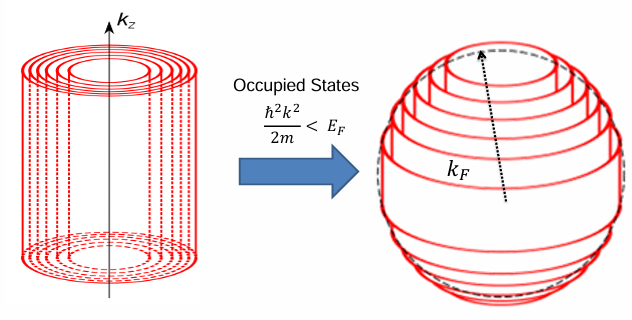
\includegraphics[width=0.8\textwidth]{images/6-Superficie-Fermi/livellilandau.png}
	\caption{I livelli di Landau rappresentano la quantizzazione del moto circolare degli elettroni nel piano per un campo magnetico applicato lungo \(z\).}
	\label{fig:livelli di Landau}
\end{figure}
\begin{figure}[H]
	\centering
	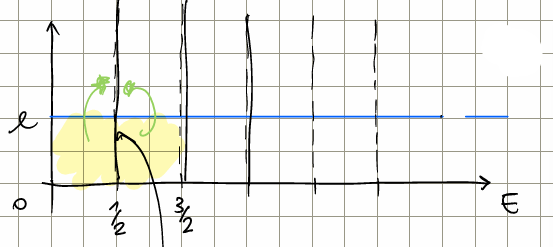
\includegraphics[width=0.6\textwidth]{images/6-Superficie-Fermi/compresslvl.png}
	\caption{Schematizzazione: l'energia contenuta nella corona d'orbite (area evidenziata) viene compressa in un livello discreto, determinato dalla quantizzazione dei livelli di Landau.}
	\label{fig:compress livelli}
\end{figure}


\subsection{Effetto Oscillatorio della Densità di Stati}

Per comprendere il comportamento oscillatorio osservato in molti esperimenti (come l'effetto De Haas--van Alphen) è fondamentale capire come il campo magnetico modifichi la densità di stati elettronici. In particolare, si studiano i casi in cui la densità di stati è calcolata in spazi di dimensioni diverse.

\subsection*{Densità degli Stati in 3 Dimensioni (3D)}

Consideriamo la relazione elementare tra la densità degli stati in \(k\)-space e in \(E\)-space.\\
In 3D il numero di stati in un volume d'elemento \(d\vec{k}\) è proporzionale a:
\[
\rho(E)dE = \rho(k) \, d\vec{k} = \rho(k) \, 4\pi k^2 \, dk\,.
\]
Dato che, per un elettrone libero, l'energia è data da:
\[
E = \frac{\hbar^2 k^2}{2m}\,,
\]
si ottiene, derivando,
\[
dE = \frac{\hbar^2}{m}\, k\, dk \quad \Longrightarrow \quad dk = \frac{m}{\hbar^2\, k}\, dE\,.
\]
Pertanto, sostituendo nell'espressione precedente, la densità degli stati per unità di energia diventa:
\[
\rho_{3D}(E)\, dE = \rho(k) \, 4\pi k^2 \, \frac{m}{\hbar^2\, k}\, dE 
= \rho(k) \, 4\pi k \,\frac{m}{\hbar^2}\, dE
\]
Concludiamo per 
\[\rho(k) = 2\cdot \biggr(\frac{L}{2\pi}\biggr)^3 \]
\[
\rho_{3D}(E) = 2\cdot \biggr(\frac{L}{2\pi}\biggr)^3 \cdot \, 4\pi \frac{m}{\hbar^2}\cdot \sqrt{\frac{2m}{\hbar^2}}\cdot \sqrt{E} = \frac{L^3}{2\pi^2}\cdot \biggr(\frac{2m}{\hbar}\biggr)^\frac{3}{2}\cdot \sqrt{E}\propto \sqrt{E}\,,
\]
ovvero la densità degli stati in 3D cresce come la radice quadrata dell'energia.
\subsection*{Densità degli Stati in 2 Dimensioni (2D)}

In 2D, il numero di stati in un elemento di area nel \(k\)-space è dato da:
\[
\rho_{2D}(E)dE = \rho(k) \, d\vec{k} = \rho(k)\, 2\pi k\, dk\,.
\]
Usiamo nuovamente la relazione energetica per un elettrone libero,
\[
E = \frac{\hbar^2 k^2}{2m} \quad \Longrightarrow \quad dk = \frac{m}{\hbar^2\, k}\,dE\,.
\]
Sostituendo:
\[
\rho_{2D}(E)\, dE = \rho(k)\, 2\pi k\, \frac{m}{\hbar^2\, k}\, dE
= \rho(k)\, 2\pi\, \frac{m}{\hbar^2}\, dE\,.
\]
Inoltre, notando che la densità dei punti in \(k\)-space per un sistema bidimensionale con condizioni periodiche è 
\[\rho(k) = 2\cdot \left(\frac{L}{2\pi}\right)^2\]
risulta che
\[
\rho_{2D}(E) = \frac{mL^2}{\pi\hbar^2}\,,
\]
cioè una quantità costante in funzione dell'energia.  \\
Pertanto, in 2D la densità degli stati è piatta (non dipende da \(E\)).

\subsection*{Densità degli Stati in 1 Dimensione (1D)}

La forma tubolare dei livelli di Landau suggerisce di considerare anche la densità di stati unidimensionale.  
In 1D, il numero di stati in un elemento \(dk\) è dato da:
\[
\rho_{1D}(E)dE = \rho(k)\, dk\,.
\]
Nei sistemi unidimensionali la densità degli stati in \(k\)-space, per condizioni periodiche, è 
\[
\rho(k) = 2\cdot \frac{L}{2\pi}\ = \frac{L}{\pi},.
\]
Per un elettrone libero la relazione energia-momento è:
\[
E = \frac{\hbar^2 k^2}{2m^*}\,,
\]
da cui
\[
dE = \frac{\hbar^2}{m^*}\, k\, dk \quad \Longrightarrow \quad dk = \frac{dE}{\frac{\hbar^2}{m^*}\, k} = \frac{m^*}{\hbar^2 k}\, dE\,.
\]
Sostituendo nell'espressione per la densità degli stati in \(k\)-space,
\[
\rho_{1D}(E)\, dE = \rho(k) \, dk = \frac{L}{\pi} \cdot \frac{m^*}{\hbar^2 k}\, dE\,.
\]
Per eliminare \(k\) in favore dell'energia, usiamo l'equazione
\[
k = \sqrt{\frac{2m^* E}{\hbar^2}}\,,
\]
quindi:
\[
\rho_{1D}(E)\, dE = \frac{L}{\pi}\, \frac{m^*}{\hbar^2\, \sqrt{\frac{2m^* E}{\hbar^2}}}\, dE
=  \frac{L}{\pi}\, \sqrt{\frac{m^*}{2\hbar^2}}\, \frac{dE}{\sqrt{E}}\,.
\]
Così si conclude che
\[
\rho_{1D}(E) \propto \frac{1}{\sqrt{E}}\,.
\]

\section{L'effetto del Campo Magnetico sui Livelli di Landau e sulla Densità degli Stati}

Nel caso in presenza del campo magnetico, gli elettroni sono quantizzati in livelli di Landau.  \\
Per ogni livello (etichettato da \(l\)), la densità di stati risulta modificata e, in particolare, per i livelli di Landau che presentano una natura unidimensionale (movimento libero lungo la direzione del campo) la densità degli stati segue il comportamento:
\[
\rho(E) \propto \frac{1}{\sqrt{E}}\,.
\]
\textbf{Questo significa che ogni volta che l'energia di Fermi \(E_F\) si avvicina al valore corrispondente a uno specifico livello di Landau, la densità degli stati mostra una divergenza (o almeno una grande fluttuazione), determinando il comportamento oscillatorio osservato negli esperimenti.  \\
Infatti, cambiando il campo magnetico (essendo \(\omega_c \propto H\)) la posizione relativa dei livelli di Landau rispetto a \(E_F\) si sposta, provocando una fluttuazione della densità degli stati all'energia di Fermi.}\\\\
Per illustrare questo punto, consideriamo la condizione per cui un elettrone a \(E_F\) occupi il livello \(l\):
\[
E_F = \hbar\omega_c\left(l+\frac{1}{2}\right) 
=\hbar\frac{eH}{m}\left(l+\frac{1}{2}\right)\,.
\]
Da qui si può ricavare:
\[
\frac{E_F}{H} = \frac{\hbar e}{m}\left(l+\frac{1}{2}\right)
\quad \Longrightarrow \quad
\frac{1}{H} = \frac{\hbar e}{mE_F}\left(l+\frac{1}{2}\right)\,.
\]
Indicando con \(A = \frac{\hbar e}{mE_F}\), per \(l=0\) abbiamo:
\[
\frac{1}{H_0} = A\frac{1}{2}\,,
\]
mentre per \(l=1\):
\[
\frac{1}{H_1} = A\frac{3}{2}\,.
\]
Queste relazioni mostrano che la distanza in \(\frac{1}{H}\) (cioè l'intervallo tra i massimi nelle oscillazioni) è determinata dall'area corrispondente alla sezione trasversale della superficie di Fermi e, in generale, varia in modo lineare con \(l+\frac{1}{2}\).\\\\
Plottando \(1/H\) si osserverà quindi una distanza costante tra i massimi, mentre variando il campo magnetico le posizioni relative dei livelli di Landau si spostano.  \\
\textbf{La "larghezza" dei tubi (ovvero delle orbite quantizzate) dipende direttamente dal campo magnetico esterno; all'aumentare di \(H\) i livelli si avvicinano a \(E_F\) e la densità degli stati mostra le divergenze caratteristiche che determinano il comportamento oscillatorio.}

\begin{figure}[H]
    \centering
    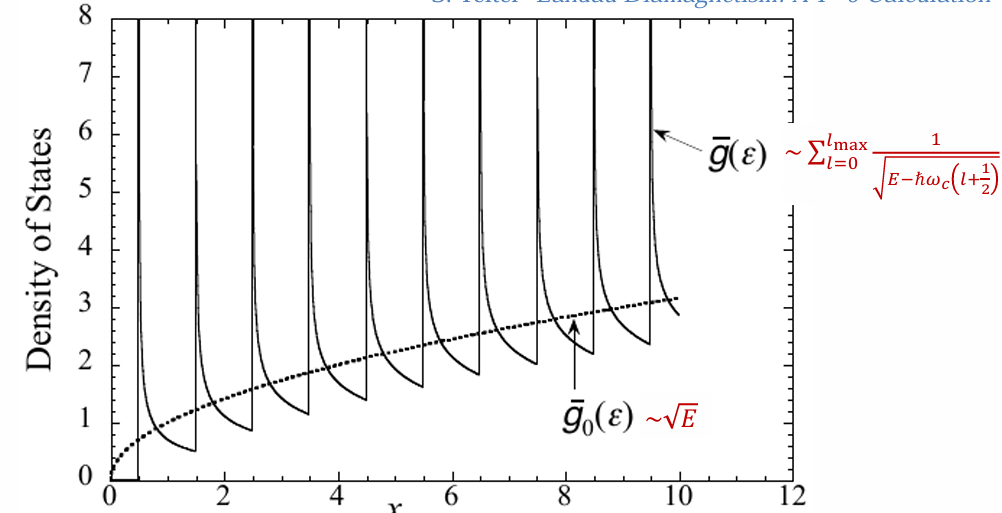
\includegraphics[width=0.9\textwidth]{images/6-Superficie-Fermi/oscillazdos.png}
    \caption{A sinistra, \(g_0(\varepsilon)\) rappresenta la densità degli stati in assenza di campo magnetico, mentre a destra \(g(\varepsilon)\) è quella in presenza del campo magnetico. Le fluttuazioni evidenziano la divergenza quando un livello di Landau si avvicina all'energia di Fermi.}
    \label{fig:oscill-dos}
\end{figure}

\bigskip
\noindent
\textbf{Conclusione:}  
Cambiando \(B\) (o, equivalentemente, \(H\)) si varia il fattore \(\omega_c\) e, di conseguenza, la posizione dei livelli di Landau rispetto a \(E_F\). Questo determina una fluttuazione della densità degli stati all'energia di Fermi, che si manifesta sperimentalmente come un comportamento oscillatorio delle proprietà magnetiche (ad es. oscillazioni in \(\frac{1}{H}\) della suscettività) e nella conduttività.  
In altre parole, la larghezza e la posizione dei "tubi" (orbite quantizzate) dipendono dal campo magnetico esterno: all'aumentare di \(H\) esse si spostano, toccando periodicamente la sfera di Fermi e generando l'oscillazione osservata.  
È importante notare che il "tubo" può intersecare la superficie di Fermi in modi differenti, dando luogo a forme particolari (come ad esempio configurazioni a "clessidra") che forniscono ulteriori informazioni sulla geometria della superficie di Fermi.




\section{Struttura delle bande}
\subsection{Metalli monovalenti}
Hanno la superficie di Fermi più semplice e si dividono in \textbf{metalli nobili} e \textbf{metalli alcalini}. Entrambi hanno un elettrone nella banda di valenza ma la loro struttura elettronica è differente.\\\\

 
 
\subsubsection{Metalli alcalini}
\textbf{I metalli alcalini} hanno la particolarità che le proprietà ottiche e di conduzione rispecchiano perfettamente il modello di Drude-Sommerfeld. Questo perchè i loro elettroni si comportano quasi come elettroni liberi (sfera di Fermi non perfetta per le perturbazioni al secondo ordine), infatti la loro banda di conduzione è formata dagli orbitali s del metallo, che si sovrappongono e creano una banda larga con una densità elettronica relativamente bassa, l'assenza di altri elettroni di valenza implica che la banda di conduzione è poco riempita e i metalli alcalini risultano essere quindi dei eccellenti conduttori.\\\\
La loro superficie di Fermi è una sfera ben contenuta nella prima zona di Brillouin, calcoliamo il raggio della sfera di Fermi che sarà dato da:
\begin{equation}
    \frac{k_F^3}{3\pi^2} = n = \frac{2}{a^3} \implies k_f = \left( \frac{3}{4\pi}\right)^{\frac{1}{3}} \left( \frac{2\pi}{a}\right) = 0,620 \left( \frac{2\pi}{a}\right) 
    \label{eqn:kappaf}
\end{equation}
che proviene dalla relazione tra $k_F$ è la densità di elettroni $n$. La distanza più breve dal centro della zona ad una delle facce (Figura \ref{fig:bcc-met-alc}) è:
\begin{equation} 
    \Gamma N = \frac{2\pi}{a} \sqrt{\left( \frac{1}{2}\right)^2 + \left( \frac{1}{2}\right)^2 + 0^2} = 0,707 \left( \frac{2\pi}{a}\right)
    \label{eqn:gamma-N}
\end{equation}
\begin{figure}
    \centering
    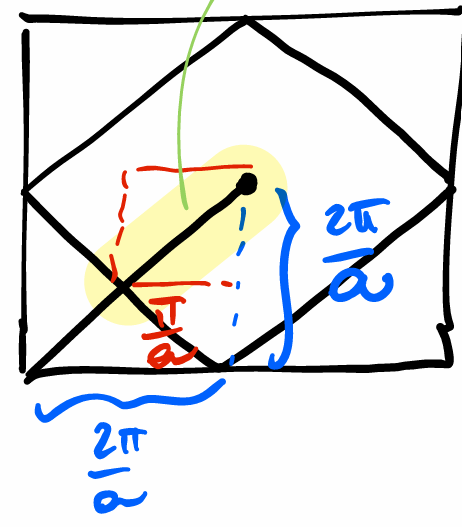
\includegraphics[width=0.2\textwidth]{images/6-Superficie-Fermi/bccmetallialk.png}
    \caption{in (\ref{eqn:gamma-N}) ho calcolato il segmento evidenziato}
    \label{fig:bcc-met-alc}
\end{figure} 

Quindi la sfera di Fermi dell'elettrone libero è interamente contenuta nella prima zona di Brillouin.\\\\
Andando a osservare il grafico in Figura \ref{fig:en-met-alc} vediamo anche che il punto in cui la perturbazione che genera il gap nelle bande è lontana dalla sfera di Fermi, questa è un'altra delle prove a favore del fatto che si comporta come un elettrone libero e questo è perché le proprietà dei metalli, come la conduttività, dipendono dagli elettroni sulla sfera di Fermi, bisgonerebbe andare al secondo ordine per vederne gli effetti. 
\begin{figure}
    \centering
    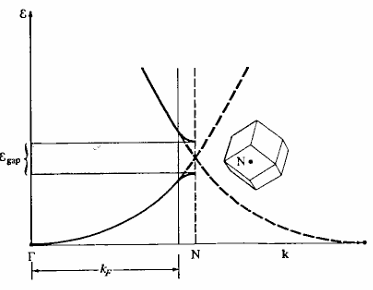
\includegraphics[width=0.7\textwidth]{images/6-Superficie-Fermi/enmetalc.png}
    \caption{}
    \label{fig:en-met-alc}
\end{figure} 

Poi misurando la superficie di Fermi tramite l'effetto di De Haas-van Alphen si conferma sperimentalmente la sfericità della sfera di Fermi in quanto si possono studiare le differenze tra una sfera di Fermi perfetta e ciò che si è ottenuto nel caso del metalli alcalini (Figura \ref{fig:sup-Fermi-met-alc} ) e sono frazioni di percentuale, quindi possiamo finalmente affermare che la loro superficie di Fermi è una sfera. 
\begin{figure}
    \centering
    \includegraphics[width=0.6\textwidth]{images/6-Superficie-Fermi/sup-Fermi-met-alc.png}
    \caption{}
    \label{fig:sup-Fermi-met-alc}
\end{figure}

\subsubsection{Metalli nobili}
\textbf{I metalli nobili} sono duttili perché sono degli FCC che si presentano a strati e quindi sono deformabili, sono caratterizzati da una banda di conduzione che è costituita principalmente dagli orbitali s e d, e le interazioni tra queste bande rendono più complessa la struttura elettronica rispetto ai metalli alcalini. \\
La banda s è larga ed è parzialmente piena (quindi conduce) e si sovrappone con la banda d che è piena, ma altamente localizzata (bassa mobilità) e  vicina in energia agli stati s, questo permette loro di ibridarsi in degli stati ibridi \textbf{sd} che modificano la dispersione (la forma della banda s). Quindi gli stati d:
\begin{itemize}
    \item non partecipano direttamente alla conduzione, ma la influenzano generando questi stati ibridi $sd$ che quando vengono eccitati (assorbimento) permettono più transizioni e quindi modificano la densità degli stati.
    \item gli stati ibridi aumentando la massa efficace degli elettroni di conduzione, questo effetto riduce la mobilità degli elettroni e, di conseguenza, la conducibilità elettrica.
    \item deformano la dipendenza di $\varepsilon$ dal momento $k$, aumenta la densità degli stati vicino all'energia di Fermi,  creando delle perturbazioni uscenti dalla superficie di Fermi che quando toccano i piani di Bragg generano dei gap, ossia aperture al primo ordine che il modello si Sommerfield non può prevedere.
\end{itemize}  
\begin{figure}
    \centering
    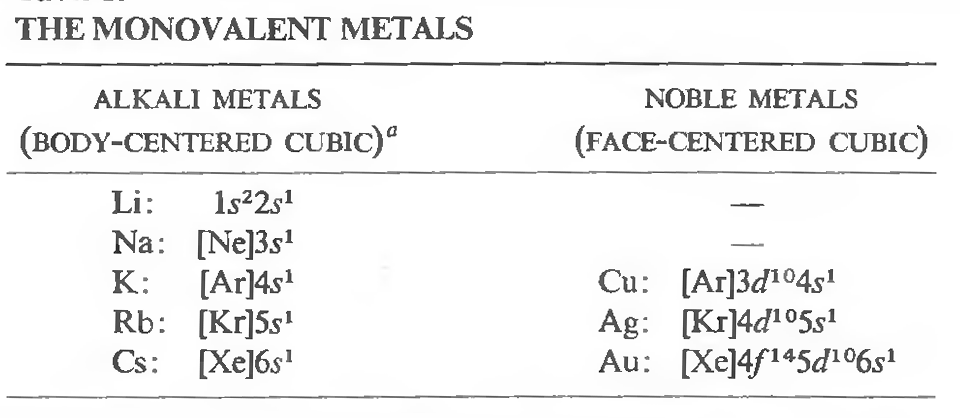
\includegraphics[width=0.9\textwidth]{images/6-Superficie-Fermi/metallimono.png}
    \caption{}
    \label{fig:metalli-monovalenti}
\end{figure} 

Dall'effeto di de Haas-van Alphen si osserva che la loro sfera di Fermi è quasi interamente sferica, però presenta dei "colli" che raggiungono le facce della BZ (Figura \ref{fig:met-nob}). Questo è un effetto di superfici minime e massime è legato alla densità di stati, i tubi in alcuni punti saranno più stretti e in altri sono più larghi, quindi sarò in punti diversi del grafico \ref{fig:oscill-dos}. Per esempio nel caso dell'oro infatti osservo due oscillazioni nella suscettività magnetica e quindi con l'effetto di de Haas-van Alphen quindi posso ottenere una superficie massima ma anche una superficie minima. 
\begin{figure} [H]
    \centering
    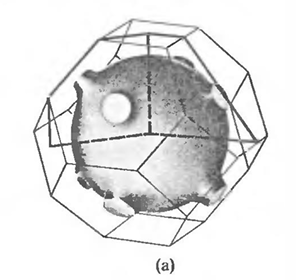
\includegraphics[width=0.3\textwidth]{images/6-Superficie-Fermi/metnob.png}
    \caption{questa è la sfera di Fermi dell'oro}
    \label{fig:met-nob}
\end{figure}


\section*{Proprietà Ottiche dei Metalli Monovalenti}

Il colore di un metallo è determinato dalla dipendenza dalla frequenza della sua riflettività, in quanto alcune frequenze della radiazione incidente vengono riflesse in misura maggiore rispetto ad altre.  
Nel semplice modello a elettrone libero non è possibile riprodurre correttamente le proprietà ottiche poiché, in assenza di collisioni, un elettrone eccitato accelera assorbendo energia e riirraggia la radiazione assorbita, riflettendola quasi completamente, il che non corrisponde alla realtà.  \\
In effetti, è proprio la presenza delle collisioni che fornisce il meccanismo per l'assorbimento dell'energia della radiazione.\\\\
Per elettroni che obbediscono alla legge di Bloch la situazione risulta differente, poiché un processo fortemente dipendente dalla frequenza della radiazione incidente diventa possibile.\\\\
Consideriamo ora un fascio di fotoni avente energia $\hbar\omega$ e momento $\hbar q$ (con il vettore d'onda del fotone $q = 2\pi/\lambda$) che eccita un elettrone da uno stato di energia $\varepsilon$ ad uno stato di energia $\varepsilon'$.  \\
I processi di assorbimento devono soddisfare le seguenti condizioni di conservazione di energia e di momento:

\begin{equation}
    \begin{split}
        \varepsilon' &= \varepsilon + \hbar\omega\,, \\
        k' &= k + q + K\,, \quad \text{con } K \in \text{Reticolo Reciproco (RL)}\,.
    \end{split}
    \label{eqn:con-en-mom}
\end{equation}

Qui si nota che il \textbf{momento cristallino} $k$ non viene conservato nel senso stretto, ma è definito modulo un vettore del reticolo reciproco, per cui
\[
k' = k \pm K\,.
\]
Questo fatto deriva dal potenziale periodico del reticolo, che introduce una perturbazione nello spazio e modifica l'operatore traslazionale collegato al momento.\\
Il meccanismo per il trasferimento di energia $\hbar\omega$ implica che l'elettrone debba passare da una banda ad un'altra (transizioni interbanda), poiché la componente di momento $q$ del fotone è molto più piccola rispetto al valore tipico del vettore d'onda degli elettroni (tipicamente $q \ll k_F$, dove $k_F$ è il raggio della sfera di Fermi).  \\
Pertanto, una transizione interbanda si verifica quando lo stato iniziale si trova al di sotto dell'energia di Fermi e lo stato finale al di sopra, e la frequenza che consente questo salto energetico è detta \textbf{frequenza di soglia}.\\\\
Nei metalli alcalini la banda completamente piena giace ben al di sotto della banda di conduzione.  
Così, l'eccitazione verso la banda di conduzione stabilisce la frequenza di soglia e, mediante un'analisi dettagliata (vedi Figura \ref{fig:trans-banda}), si ottiene la relazione

\[
\hbar\omega = \frac{\hbar^2}{2m}\,(2k_0 - k_F)^2 - \frac{\hbar^2}{2m}\, k_F^2\,,
\]
dove $k_0$ è la distanza (calcolata, ad esempio, lungo la direzione $\Gamma N$ come visto in precedenti analisi) e, sperimentalmente, si trova che $k_F \approx 0,877\, k_0$.  
Da questa relazione si ottiene:
\[
\hbar\omega \approx 0,64\, \varepsilon_F\,,
\]
con $\varepsilon_F$ che indica l'energia di Fermi.

\begin{figure}[H]
    \centering
    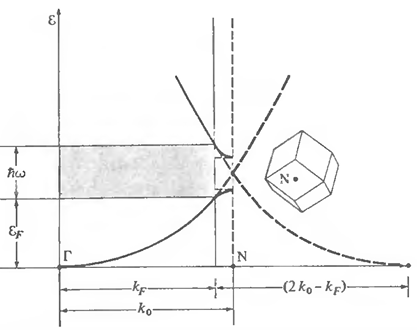
\includegraphics[width=0.6\textwidth]{images/6-Superficie-Fermi/transbanda.png}
    \caption{Schema delle transizioni interbanda in un metallo alcalino.}
    \label{fig:trans-banda}
\end{figure}
\begin{figure}[H]
    \centering
    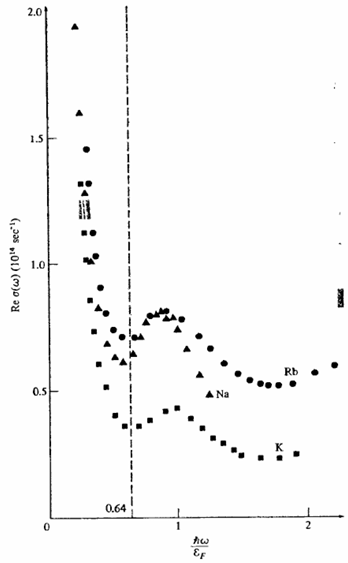
\includegraphics[width=0.6\textwidth]{images/6-Superficie-Fermi/trasm-met-alc.png}
    \caption{Grafico della trasmittanza di alcuni metalli alcalini: si osserva un assorbimento significativo in un intorno di $0,64\,\varepsilon_F$, dove $\varepsilon_F$ è l'energia di Fermi dell'elettrone libero.}
    \label{fig:trasmittanza}
\end{figure}

\section{Metalli Bivalenti e Trivalenti}

\subsection{Metalli Bivalenti}
I metalli divalenti sono quelli la cui struttura elettronica porta ad avere una banda di conduzione parzialmente occupata.  
In Figura \ref{fig:metalli-divalenti} sono riportati alcuni esempi di metalli divalenti.

\begin{figure}[H]
    \centering
    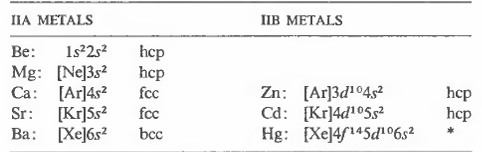
\includegraphics[width=0.7\textwidth]{images/6-Superficie-Fermi/metallidiv.png}
    \caption{Esempi di metalli divalenti.}
    \label{fig:metalli-divalenti}
\end{figure}

\subsection{Metalli Trivalenti}
Tra i metalli trivalenti il caso più semplice è rappresentato dall'alluminio.  
Nel caso dell'alluminio, la prima zona di Brillouin è completamente piena e contiene due elettroni per atomo; il terzo elettrone, invece, si distribuisce nelle seconde e terze zone.  
Si consideri la seguente analisi:

\[
n_e^{II} + n_e^{III} = \frac{n}{3}\,,
\]
dove $n$ è la densità complessiva di elettroni liberi e la suddivisione per 3 deriva dal fatto che, mediamente, vi è un elettrone per cella elementare in eccesso oltre a quelli che occupano la prima zona.  
Inoltre, considerando che in ciascuna zona sono ammessi al massimo due elettroni (degenerazione per spin), si ha:
\[
n_e^{II} + n_h^{II} = 2 \left(\frac{n}{3}\right)\,.
\]
Sottraendo queste due relazioni si ottiene:
\[
n_e^{III} - n_h^{II} = -\frac{n}{3}\,.
\]
Questo risultato indica che, dal punto di vista della conduzione, l'alluminio trasporta una lacuna per atomo.


\chapter{Energia di Coesione e Classificazione dei Solidi}

\section{Classificazione dei Solidi}

A differenza del capitolo precedente, in cui i solidi sono stati descritti principalmente in base alla struttura geometrica, in questo capitolo si classificheranno i solidi in base alla configurazione degli elettroni in valenza.  
La distinzione principale viene fatta tra metalli e isolanti e si basa sulla distribuzione elettronica nello spazio $k$.  
Nei metalli si osserva la presenza di bande semipiene, mentre negli isolanti gli elettroni risultano fortemente localizzati.

\subsection{Isolanti}
Gli isolanti possono essere classificati in tre gruppi:
\begin{itemize}
    \item \textbf{Cristalli covalenti:} in cui la distribuzione elettronica è molto localizzata lungo direzioni ben definite, legata alla formazione dei legami covalenti.
    \item \textbf{Cristalli molecolari:} per esempio, i gas nobili allo stato solido, caratterizzati da shell elettroniche completamente piene.
    \item \textbf{Cristalli ionici:} dove l'interazione principale è di natura coulombiana, dovuta alla presenza di ioni.
\end{itemize}

\subsection{Cristalli Alogenuro-Alcalini}
I cristalli alogenuro-alcalini sono cristalli ionici formati da un catione (tipicamente un metallo alcalino) e un anione (tipicamente un alogeno).  
La stabilità di tali solidi è dovuta al potenziale coulombiano che si instaura tra ioni di carica opposta.  
Per fare un esempio, consideriamo il cristallo di \ce{RbBr}:  \\
per formare uno ione \ce{Br-} è necessaria un'energia di circa \SI{-3.5}{\electronvolt}, mentre per formare uno ione \ce{Rb+} occorrono circa \SI{4.2}{\electronvolt}.  
Apparentemente, un atomo di Rb legato a un atomo di Br implicherebbe un consumo netto di energia di circa \SI{0.5}{\electronvolt}.  
Tuttavia, abbassando la distanza tra gli ioni, l'interazione elettrostatica riduce significativamente l'energia, così che nel cristallo \ce{RbBr}, per una distanza tipica di $r \approx$ \SI{0.34}{\nano\meter}, l'energia coulombiana raggiunge valori di circa \SI{-4.2}{\electronvolt}, compensando ampiamente il contributo energetico positivo.\\
La struttura reticolare dei cristalli alogenuro-alcalini è confermata anche da diffrazioni a raggi X.  
In Figura \ref{fig:NaCl-cristallo} è riportata la densità di carica elettronica per il caso dell'\ce{NaCl}.
\begin{figure}[H]
    \centering
    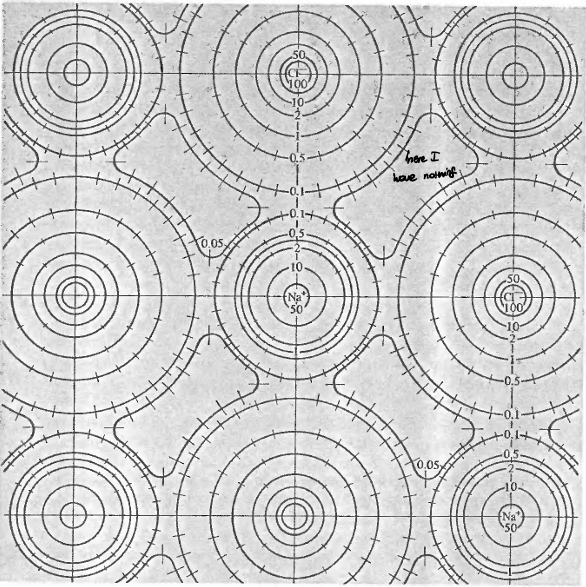
\includegraphics[width=0.5\textwidth]{images/7-Classificazione-Solidi/cristNaCl.png}
    \caption{Densità di carica elettronica nell'NaCl.}
    \label{fig:NaCl-cristallo}
\end{figure}

Dal punto di vista elettronico, essendo degli isolanti, questi cristalli presentano un ampio gap tra la banda di valenza e quella di conduzione.  
Inoltre le bande sono molto piatte, il che implica che la derivata seconda dell'energia rispetto al vettore d'onda è piccola.  
Questo porta a una massa efficace elevata e, conseguentemente, a una bassa mobilità degli elettroni, come si evince dal grafico in Figura \ref{fig:bande-alk-hal}.

\begin{figure}[H]
    \centering
    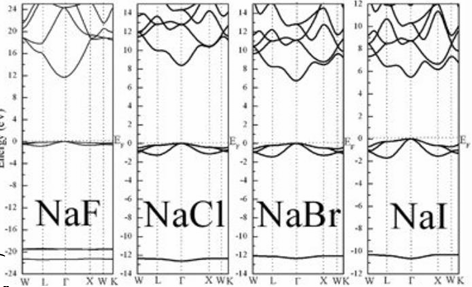
\includegraphics[width=0.5\textwidth]{images/7-Classificazione-Solidi/bandealkhal.png}
    \caption{Bande elettroniche nei cristalli alogenuro-alcalini: bande piatte che indicano una bassa mobilità elettronica.}
    \label{fig:bande-alk-hal}
\end{figure}

\noindent
Confrontando la distanza tra due ioni in un cristallo ionico con la metà della distanza tra il primo vicino in un metallo (vedi Figura \ref{fig:dist-metalli}), si osserva che nei cristalli ionici gli ioni sono molto più vicini tra loro rispetto agli atomi in un metallo.  
Questo fatto solleva il problema: \emph{che cosa tiene insieme un metallo?}  
La risposta risiede negli effetti puramente quantistici derivanti dall'interazione degli elettroni, che stabilizzano il reticolo metallico anche se gli atomi sono più distanziati.

\begin{figure}[H]
    \centering
    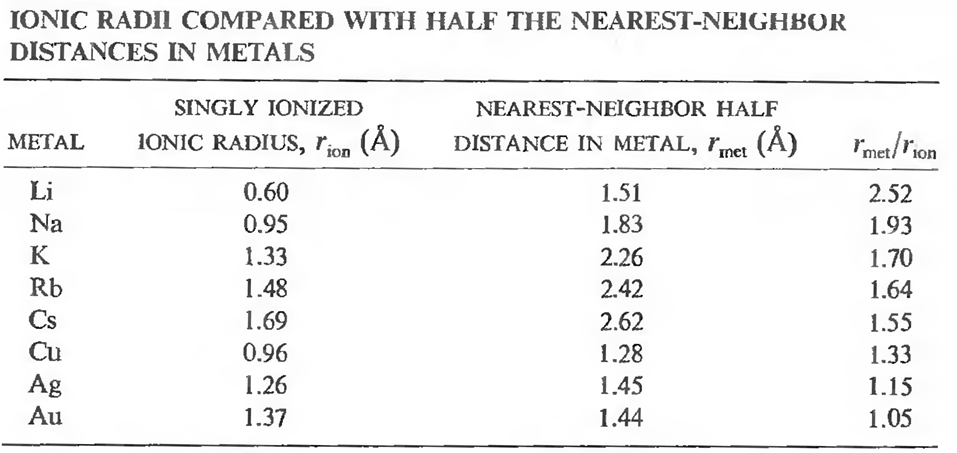
\includegraphics[width=0.8\textwidth]{images/7-Classificazione-Solidi/Distmetalli.png}
    \caption{Confronto tra le distanze interatomiche nei metalli e negli ioni in un cristallo ionico.}
    \label{fig:dist-metalli}
\end{figure}


\section{Energia di Coesione}
L'energia di coesione è l'energia necessaria per estrarre un atomo dal cristallo, vediamo l'energia di coesione nei diversi tipi di solido.
\subsection{Forze di Van Der Waals e potenziale di Lennard-Jones}
Le forze di Van der Waals sono forze di attrazione o repulsione deboli che si manifestano tra molecole (o atomi) neutri, non legate da legami chimici covalenti o ionici. Sono fondamentali per spiegare molti fenomeni fisici e chimici, come la condensazione dei gas, la coesione tra molecole nei liquidi e il comportamento delle molecole biologiche.\\\\
Come si orginano? Supponiamo di avere due atomi ad una distanza $r$, anche se la loro distribuzione di carica media è simmetrica, possiamo avere fluttuazioni istantanee che genererano un momento di dipolo istantaneo $p_1$ con un campo elettrico $E \propto \frac{p_1}{r^3}$. Quest'ultimo a sua volta indurrà un momento di dipolo istantaneo nell'atomo 2 che sarà pari a $ p_2 = \alpha E \sim \frac{\alpha p_1}{r^3}$, con $\alpha$ polarizzabilità, ossia la misura della deformazione di carica.\\
L'energia potenziale dovuta all'interazione tra i due dipoli sarà data da:
\[ \frac{p_2 p_1}{r^2} \sim \frac{\alpha p_1^2}{r^6}\]
Dimostriamolo usando la meccanica quantistica: \\
considera la situazione riportata in Figura \ref{fig:dip}
\begin{figure} [H]
    \centering
    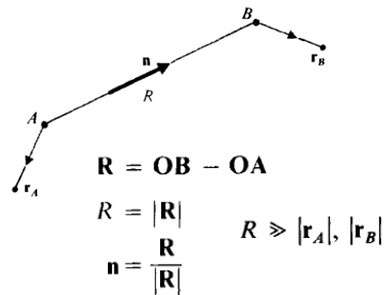
\includegraphics[width=0.5\textwidth]{images/7-Classificazione-Solidi/dip.png}
    \caption{}
    \label{fig:dip}
\end{figure} 

Il dipolo è dato da:
\[ \begin{split}
    &\mathcal{D}_A = qr_A \\
    &\mathcal{D}_B = qr_B \\
\end{split}\]
L'energia potenziale di un dipolo in un campo elettrico è:
\[ U(\mathbf{R}) = \frac{1}{4\pi\varepsilon_0} \frac{\mathcal{D}_A\cdot \mathbf{R}}{R^3}\]
Quindi:
\[ \mathbf{E} = -\nabla_R U = -\frac{q}{4\pi\varepsilon_0}\frac{1}{R^3}[\mathbf{r}_A-3(\mathbf{r}_A \cdot \mathbf{n})\mathbf{n}]\]
ora andiamo a vedere l'interazione del campo elettrico generato dal dipolo $\mathcal{D}_A$ con il dipolo $\mathcal{D}_B$, quindi dato $r_{A,B} = x_{A,B} \hat{i}+y_{A,B}\hat{j}+z_{A,B}\hat{k}$ otteniamo:
\[
\begin{split}
    &\mathcal{W}_{dd} = - \mathbf{E} \cdot \mathcal{D}_B = \frac{e^2}{R^3}[ \mathbf{r}_A \cdot \mathbf{r}_B - 3(\mathbf{r}_A \cdot \mathbf{n})(\mathbf{r}_B \cdot \mathbf{n})] \\
    & \implies \mathcal{W}_{dd} = \frac{e^2}{R^3}(x_Ax_B + y_Ay_B - 2z_Az_B)
\end{split}
\]
Ora trasformiamo questo approccio classico in un operatore quantistico
\begin{equation}
    \mathcal{W}_{dd} = \frac{e^2}{R^3} (X_AX_B + Y_AY_B -2Z_AZ_B)
    \label{eqn:quantum-wdd}
\end{equation}
dove in questo caso $X$ è l'operatore posizione associato al dipolo. L'hamiltoniana sarà: 
\[H = H_{0A}+H_{0B} + \mathcal{W}_{dd}\]
dove le $H_0$ sono le hamiltoniane atomiche e $\mathcal{W}_{dd}$ è la parte di interazione, quindi utilizzo la teoria delle perturbazioni:
\[(H_{0A}+H_{0B})\ket{\psi_{n,l,m}^A; \psi_{n',l',m'}^B} = (E_n + E_{n'})\ket{\psi_{n,l,m}^A; \psi_{n',l',m'}^B} \]
Allo stato fondamentale imperturbato l'energia sarà la somma dell'energia dei due stati fondamentali dei due singoli atomi $E_T = -2E_0$.\\
Mentre la perturbazione al primo ordine sarà:
\[ \varepsilon_1 = \bra{\psi_{1,0,0}^A;\psi_{1,0,0}^B}\mathcal{W}_{dd}\ket{\psi_{1,0,0}^A;\psi_{1,0,0}^B} = 0\]
Questo perché è il prodotto dei termini \\
\[\bra{\psi_{1,0,0}^A;\psi_{1,0,0}^B} X_A \ket{\psi_{1,0,0}^A;\psi_{1,0,0}^B}\bra{\psi_{1,0,0}^A;\psi_{1,0,0}^B}X_B\ket{\psi_{1,0,0}^A;\psi_{1,0,0}^B} = 0\]
in quanto allo stato stazionario il  valore medio delle componenti degli operatori di posizione è zero.\\
Quindi dobbiamo andare al secondo ordine:
\begin{equation*}
\varepsilon_2 = \sum_{\substack{n,l,m \\ n',l',m'}} \frac{|\bra{\psi_{n,l,m}^A;\psi_{n',l',m'}^B} \mathcal{W}_{dd}\ket{\psi_{1,0,0}^A;\psi_{1,0,0}^B}|^2}{-2E_1-E_n-E_{n'}}
\end{equation*}
data (\ref{eqn:quantum-wdd}) estraggo $\left| \frac{1}{R^3} \right|^2$ dalla somma e ottengo:
\[ \varepsilon_2 = - \frac{C}{R^6}\]
dove C è il numero che sarà dato da $\bra{...}\mathcal{W}_{dd}\ket{...}$ senza $1/R^3$. \\
\textbf{Quindi possiamo concludere che le forze di Van der Waals sono di tipo attrattivo (segno meno) e sono date dal secondo ordine perturbativo dell'energia.}
\\~\\
Quando gli atomi si avvicinano però entra in gioco la repulsione dei nuclei atomici, quindi il potenziale che descrive al meglio il sistema in modo più semplice possibile è quello di \textbf{Lennard-Jones} (Figura \ref{fig:lennard-jones}). La relazione che descrive questo potenziale è stata ottenuta tramite  un approccio semi empirico fittando dati sperimentali
\[ \phi(r) = -\frac{A}{r^6} + \frac{B}{r^{12}}\]
dove il primo termine indica l'attrazione dovuta alle forze di Van der Waals e il secondo è la repulsione dei nuclei. Il fatto che sia alla 12esima potenzia il termine repulsivo non ha alcun significato fisico, viene dal fit ed è arbitrario, semplicemente serviva qualcosa che divergesse velocemente su piccole distanze. \\
Un altro modo per scrivere questa relazione è:
\begin{equation}
\begin{split}
 &\phi(r) = 4\varepsilon \left[ \left( \frac{\sigma}{r}\right)^{12} - \left( \frac{\sigma}{r}\right)^6 \right] \\
 & \sigma = \left( \frac{B}{A}\right)^{\frac{1}{6}} \\
 & \varepsilon = \frac{A^2}{4B}
\end{split}
\label{eqn:lennard-jones-pot}
\end{equation}
dove $\varepsilon$ è un parametro che ha le dimensioni di un'energia ed è relativo all'energia di coesione mentre $\sigma$ ha le dimensioni di una lunghezza ed è legato alla distanza media tra due atomi.
\begin{figure} [H]
    \centering
    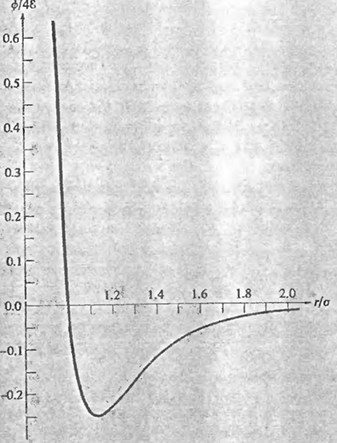
\includegraphics[width=0.4\textwidth]{images/7-Classificazione-Solidi/lennardjones.png}
    \caption{}
    \label{fig:lennard-jones}
\end{figure}
\begin{figure} [H]
    \centering
    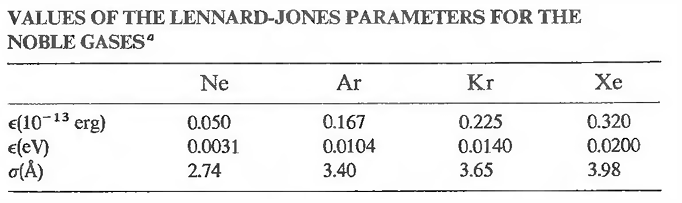
\includegraphics[width=0.75\textwidth]{images/7-Classificazione-Solidi/valori-lennard-jones.png}
    \caption{}
    \label{fig:valori-lennard-jones}
\end{figure}

Ora troviamo l'energia potenziale totale del solido. \\
L'energia di interazione totale di un atomo all'origine con tutti gli altri è data da:
\[ \sum_{\mathbf{R} \neq 0} \phi (\mathbf{R})\]
($R \neq 0$ perché non ho self interaction) \\
Quindi l'energia per singola particella è data da:
\begin{equation}
    u = \frac{1}{2} \sum_{\mathbf{R} \neq 0} \phi (\mathbf{R})
    \label{eqn:ulj}
\end{equation}
dove l'$1/2$ serve per evitare di contare 2 volte la stessa coppia di atomi. Quindi l'energia totale sarà quest'ultima per il numero N di particelle $\implies U = Nu$. \\
Conviene considerare R nel seguente modo:
\[ |\mathbf{R} | = \alpha(\mathbf{R}) r
\]
dove r è la distanza dell'atomo con i primi vicini e $\alpha(\mathbf{R})$ è un parametro che dipende dalla tipo di reticolo e ci dice che la posizione degli atomi è sempre nella stessa direzione nel solido. Quindi la (\ref{eqn:ulj}) inserendo (\ref{eqn:lennard-jones-pot}) con questo $R$ diventa:
\[ 
\begin{split}
&u = 2\varepsilon \left[ A_{12} \left( \frac{\sigma}{r}\right)^{12} - A_6 \left( \frac{\sigma}{r}\right)^6 \right] \\
&A_n = \sum_{R \neq 0} \frac{1}{\alpha(R)^n}
\end{split}
\]
$A_n$ è un termine che dipende quindi dal tipo di cristallo, alcuni valori sono riportati in Figura \ref{fig:valori-An}
\begin{figure} [H]
    \centering
    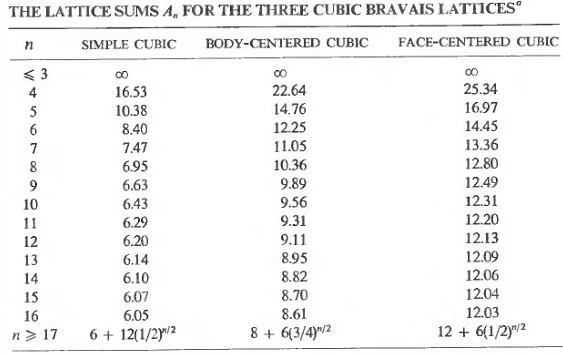
\includegraphics[width=0.75\textwidth]{images/7-Classificazione-Solidi/valoriAn.png}
    \caption{l'esponente deve essere maggiore di 3 altrimenti la serie non converge}
    \label{fig:valori-An}
\end{figure}

Posso trovare la distanza tra due atomi all'equilibrio facendo $\frac{\partial u}{\partial r} = 0$ e si ottiene
\[ r_0^{th} = \left( \frac{2A_{12}}{A_6} \right)^{\frac{1}{6}}\sigma = 1,09\sigma\]
Quindi all'equilibrio è:
\[ u_0^{th} = -\frac{\varepsilon A_6^2}{2A_{12}} = -8,6\varepsilon\]
Possiamo anche calcolare il \textbf{modulo di compressibilità} all'equilibrio che sarà dato da:
\[ \begin{split}
    &B = - V \left( \frac{\partial P}{\partial V}\right)_T \\
    & P = -\frac{dU}{dV}, \ \ v = \frac{V}{N} \\
    & B = v \frac{\partial}{\partial v}\left( \frac{\partial u}{\partial v}\right)_T
\end{split} \]
per un FCC (vedi Figura \ref{fig:FCC}) che ha lato di lunghezza $a$, la distanza di un atomo col suo primo vicino sarà data da $r$ ed è la diagonale di un quadrato di lato $a/2$. Perciò $a = \sqrt{2}r$ e ho 4 celle unitarie quindi:
\[v = \frac{a^3}{4} = \frac{r^3}{\sqrt{2}} \implies \frac{\partial }{\partial v} = \frac{\partial}{\partial r}\frac{\partial r}{\partial v} = \frac{\sqrt{2}}{3r^2}\frac{\partial}{\partial r}\]
B quindi diventa:
\[ B = \frac{r^3}{\sqrt{2}} \frac{\sqrt{2}}{3r^2} \frac{\partial}{\partial r} \frac{\sqrt{2}}{3r^2}\frac{\partial u}{\partial r} = \frac{\sqrt{2}}{9} r \frac{\partial}{\partial r}\frac{1}{r^2}\frac{\partial u}{\partial r}\]
se $r = r_0^{th} \equiv r_0$ abbiamo che 
\[ \begin{split}
     &B = \frac{\sqrt{2}}{9} r_0 \frac{\partial}{\partial r}\frac{1}{r_0^2}\frac{\partial u}{\partial r} = \frac{\sqrt{2}}{9} \frac{\cancel{r_0}}{r_0^{\cancel{2}}}\frac{\partial}{\partial r}\frac{\partial u}{\partial r} =\\
     & = \frac{\sqrt{2}}{9r_0}\left(\frac{\partial^2 u}{\partial r^2}\right)_{r=r_0} = \frac{4\varepsilon}{\sigma^3} A_{12} \left( \frac{A_6}{A_{12}} \right)^{\frac{5}{2}} = \frac{75\varepsilon}{\sigma^3}
    \end{split}\]

\subsection{Cristalli ionici}
Siccome un cristallo ionico è formato da ioni positivi e negativi che si alternano, ciascun ione sarà attratto da alcuni e respinto da altri in un suo intorno, perciò l'energia di coesione sarà data da due contributi: uno attrattiva coulombiano e uno repulsivo con i nuclei quando gli atomi si avvicinano troppo.
\[ u(r) = u^{\text{core}}(r) + u^{\text{coul}}(r) \]
Ci sarebbe anche da aggiungere il contributo delle forze di Van der Waals ma in questo caso sono trascurabili. \\\\
In questo caso $u^{\text{coul}}(r)$ è molto difficile da calcolare perché ho interazioni sia repulsive che attrattive. Considero l'esempio dell'\textbf{\ce{NaCl}} cristallo composto da 2 reticoli di Bravais FCC sovrapposti, uno composto da ioni negativi in posizione $\mathbf{R}$ e un secondo composto da ioni positivi spostato di \textbf{d} (vedi Figura \ref{fig:NaCl} e considera i pallini neri come ioni negativi e quelli bianchi come ioni positivi). \\
In un  FCC la distanza tra i primi vicini è data da $r = \frac{a}{2}$, quindi come prima si ottiene
\[ \begin{split} &|\mathbf{R}| = \alpha(R) r \ \ \ \  \text{reticolo fcc negativo} \\
& |\mathbf{R + d}| = \alpha(R+d) r \ \ \ \  \text{reticolo fcc positivo}
\end{split}
\]
Quindi il potenziale di un singolo anione o catione sarà:
\begin{equation}
    u^{\text{coul}}(r) = -\frac{e^2}{r} \left\{ \frac{1}{\alpha(d)} + \sum_{R \neq 0} \left( \frac{1}{\alpha(R + d)} - \frac{1}{\alpha(R)}\right)\right\}
    \label{eqn:ucoul}
\end{equation}
dove il primo termine è l'interazione attrattiva degli atomi all'interno di una cella, mentre tutto il resto è l'interazione con tutti gli altri ioni di tutte le altre celle. L'energia totale sarà
\[ U = - \frac{N}{2}\frac{e^2}{r} \left\{ \frac{1}{\alpha(d)} + \sum_{R \neq 0} \left( \frac{1}{\alpha(R + d)} - \frac{1}{\alpha(R)}\right)\right\}\]

\subsubsection{Costante di Madelung}
La (\ref{eqn:ucoul}) può essere scritta così:
\[ u^{\text{coul}}(r) = -\alpha_M \frac{e^2}{r}\]
Nel caso 1 dimensionale la situazione è la seguente:
\begin{figure} [H]
    \centering
    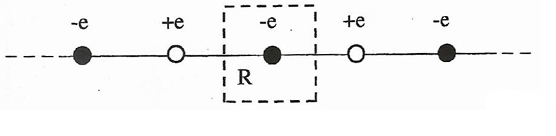
\includegraphics[width=0.75\textwidth]{images/7-Classificazione-Solidi/madel1d.png}
    \caption{}
    \label{fig:madel-1d}
\end{figure} 

Sviluppo la serie della (\ref{eqn:ucoul}) e diventa:
\[ u^{\text{coul}}(r) = - \frac{e^2}{2}2\left[\frac{1}{1}-\frac{1}{2}+\frac{1}{3}-\frac{1}{4}+\frac{1}{5}-...\right] = -\frac{e^2}{r}2\ln 2\]
Quindi la costante di Madelung è: $\alpha_M = 2 \ln 2$. Il numero 2 all'interno del logaritmo sta a indicare che le particelle coinvolte sono due. A dimensioni superiori l'interazione si fa più complicata e la serie potrebbe essere non ben definita e quindi divergere. \\
\textbf{L'idea di madelung è stata comprendere che la sommatoria dipende da come viene costruito il cristallo, introduce quindi delle interazioni quadrupolo suddividendo il cristallo in celle elettricamente neutre e a simmetria cubica nelle quali l'interazione elettrostatica cade rapidamente (come l'inverso della quinta potenza $\sim 1/r^5$) e in seguito calcola l'energia di interazione in ogni cella e tra le celle. }\\\\
Ogni cella contiene:\\
a)  4 unità di carica positiva composte da: $\frac{1}{1}$ una unità intera al centro e $\frac{12}{4}$ dodici quarti sui bordi \\
b)  4 unità di carica negativa composte da: $\frac{6}{2}$ sei metà (1 per ogni faccia) e $\frac{8}{8}$ otto ottavi sugli angoli, come in Figura \ref{fig:madel-3d}.
\begin{figure} [H]
    \centering
    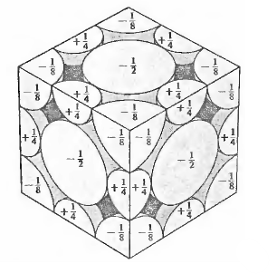
\includegraphics[width=0.4\textwidth]{images/7-Classificazione-Solidi/madel3d.png}
    \caption{}
    \label{fig:madel-3d}
\end{figure} 

Quindi l'interazione ora è divisa nell'interazione di una cella con tutte le altre e nell'interazione interna alla cella invece che l'atomo con tutti gli altri.\\
\[u = u_{\text{cell}}+u_{\text{int}}\]
La cella al suo interno ha delle interazioni di \textbf{quadrupolo} perché ho una carica centrale che interagisce con 4 cariche attorno. Quindi la serie diventa:
\[ u^{\text{coul}}(r) = -\frac{e^2}{r}\left[ \frac{6}{1}-\frac{12}{\sqrt{2}}+\frac{8}{\sqrt{3}}-\frac{3}{\sqrt{4}}+\frac{12}{\sqrt{5}}-\frac{12}{\sqrt{6}}-\frac{3}{\sqrt{8}}+\frac{6}{\sqrt{9}}-\frac{1}{\sqrt{12}}\right] = - 1,751 \frac{e^2}{r}\]
quindi $\alpha_M = 1,751$. \\
Siccome è poco diversa da 1 vuol dire che l'interazione con tutto il resto non è poi così importante, quasi tutta l'interazione coulombiana è ristretta alla cella elementare. 
\\~\\
Ora aggiungiamo a $u^{\text{coul}}(r)$ la repulsione dei nuclei che può essere rappresentata come qualcosa che varia rapidamente al variare della distanza tra gli ioni (la possiamo vedere come una correzione all'energia), quindi l'energia totale è:
\[ u(r) = - \frac{\alpha e^2}{r} + \frac{C}{r^m}\]
Per trovare la separazione all'equilibrio $r_0$ dobbiamo minimizzare $u(r)$ ponendo $\frac{\partial u}{\partial r} = 0$
\[ \begin{split}
    &r_0^{m-1} = \frac{mC}{e^2 \alpha} \implies C = \frac{\alpha e^2 r_o^{m-1}}{m} \\
    &u_0^{th} \equiv u(r_0) = -\frac{\alpha e^2}{r_0}\frac{m-1}{m} \\
    & m = 1 + \frac{18 B_0 r_0^3}{|u^{\text{coul}}(r_0)|}
    \end{split}
\]
dove $B_0$ è il modulo di compressibilità (bulk modulus). \\\\
\textbf{Dai valori riportati nella tabella in Figura \ref{fig:valori-ci} si nota che l'80\%-90\% dell'energia di coesione dei cristalli ionici è attrazione coulombiana, la correzione è veramente piccola.}
\begin{figure} [H]
    \centering
    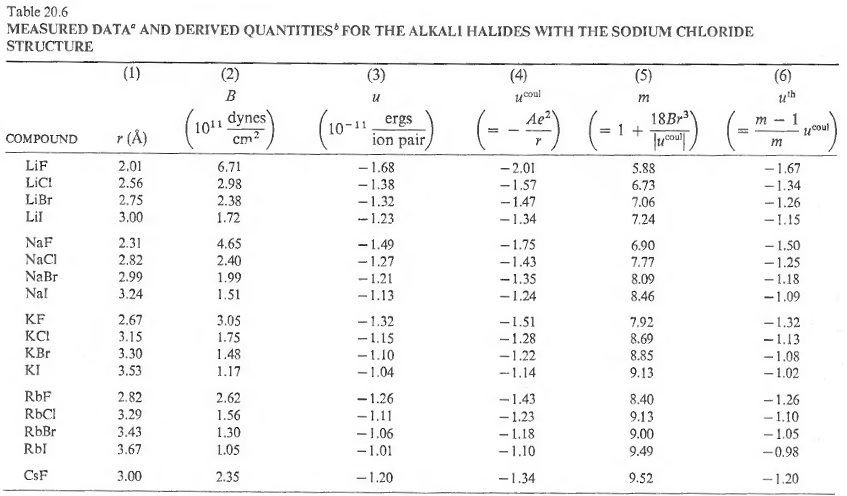
\includegraphics[width=\textwidth]{images/7-Classificazione-Solidi/valori-en-crist-ionici.png}
    \caption{}
    \label{fig:valori-ci}
\end{figure}

\subsection{Metalli}
Per i metali, ossia solidi ionici non covalenti, possiamo considerare un reticolo formato da ioni (positivi) fissi con una distribuzione degli elettroni di valenza uniforme su tutto il solido. \\
Quindi abbiamo che l'energia totale sarà data dalla somma dell'energia delle cariche puntiformi positive dei nuclei del metalle e dall'energia di un gas di elettroni con una densità di $\frac{3}{4}\pi r_s^3$ dove $r_s$ dipende dalla densità ed è dato da: $\frac{1}{n} = 4\pi r_s^3$, quindi 2 volte la distanza tra gli elettroni, e $n = \frac{N_e}{V}$ dove $N_e$ è il numero di elettroni di valenza.\\
Quindi l'energia totale è:
\[u^{\text{coul}} = - \frac{24.35}{(r_s/a_0)}  \ \ \ \text{eV/atomo}\]
L'energia è legata all'energia di Fermi $\varepsilon_F$, quindi calcoliamo l'energia cinetica:
\[ u^{\text{kin}} = \frac{3}{5}\varepsilon_F = \frac{30.1}{(r_s/a_0)^2} \ \ \text{eV/atomo}\]
è più alta dell'energia attrattiva quindi \textbf{c'è qualcosa che tiene il metallo stabile, questo significa che ci sono degli effetti quantistici e l'energia associata a questo è l'exchange energy}
\[ \begin{split}
    &u^{ex} = - \frac{12.5}{(r_s/a_0)} \ \ \text{eV/atomo} \\
    &\implies u = u^{kin} +u^{\text{coul}} + u^{ex} = \left[ \frac{30.1}{(r_s/a_0)^2} - \frac{24.35}{(r_s/a_0)} - \frac{12.5}{(r_s/a_0)} \right] \ \ \text{eV/atomo}  =\\
    & = \frac{30.1}{(r_s/a_0)^2} - \frac{36.8}{(r_s/a_0)} \ \ \text{eV/atomo} 
    \end{split}
\]
Minimizzando questa rispetto a $r_s$ troviamo:
\[ \frac{r_s}{a_0} = 1.6\]



\chapter{Fononi}
\section{Cristallo Armonico "Classico"}
Consideriamo un reticolo di Bravais in cui ogni sito occupato da uno ione non è fisso, ma vibra attorno alla propria posizione di equilibrio. Indichiamo la posizione reale dell'ione con
\[
\vec{r}(\vec{R}) = \vec{R} + \vec{u}(\vec{R}),
\]
dove \(\vec{R}\) è la posizione di equilibrio (proveniente dal reticolo di Bravais) e \(\vec{u}(\vec{R})\) è lo spostamento (con \(|\vec{u}(\vec{R})| \ll a\), dove \(a\) è la distanza interatomica).\\\\
Si assume inoltre l'\textbf{approssimazione adiabatica}, vale a dire che la scala temporale degli elettroni è molto più veloce di quella degli ioni. In questo modo, gli elettroni occupano sempre lo stato fondamentale per una data configurazione ionica, permettendo di disaccoppiare le dinamiche elettronica e ionica.\\\\
L'Hamiltoniana del sistema è data da
\[
H = \sum_{\vec{R}} \frac{\vec{P}(\vec{R})^2}{2M} + U,
\]

\subsection*{Energia Potenziale del Reticolo}
Nel caso statico, cioè quando le ioni restano fissi nelle posizioni di equilibrio, l'energia potenziale si ottiene considerando un potenziale a due corpi:
\[
U = \frac{1}{2}\sum_{\vec{R},\vec{R}'} \phi(\vec{R}-\vec{R}') = \frac{N}{2}\sum_{\vec{R}} \phi(\vec{R}),
\]
dove \(N\) è il numero totale di ioni.\\
Nel caso dinamico, dove gli ioni sono spostati dalle loro posizioni di equilibrio, abbiamo:
\[
U = \frac{1}{2}\sum_{\vec{R},\vec{R}'} \phi\Bigl(\vec{r}(\vec{R}) - \vec{r}(\vec{R}')\Bigr)
= \frac{1}{2}\sum_{\vec{R},\vec{R}'} \phi\Bigl(\vec{R} - \vec{R}' + \vec{u}(\vec{R}) - \vec{u}(\vec{R}')\Bigr).
\]
Poiché \(|\vec{u}(\vec{R})| \ll |\vec{R}|\), è possibile espandere il potenziale in serie di Taylor attorno a \(\vec{u}=0\). Si ottiene:
\begin{equation}
\begin{split}
    U &\approx \frac{N}{2}\sum_{\vec{R} \neq 0}\phi(\vec{R}) \\
    &\quad + \frac{1}{2}\sum_{\vec{R},\vec{R}'} \Bigl\{ \bigl[\vec{u}(\vec{R}) - \vec{u}(\vec{R}')\bigr] \cdot \vec{\nabla} \phi(\vec{R}-\vec{R}') \Bigr\} \\
    &\quad + \frac{1}{4}\sum_{\vec{R},\vec{R}'} \Bigl\{ \bigl[\vec{u}(\vec{R}) - \vec{u}(\vec{R}')\bigr] \cdot \nabla^2 \phi(\vec{R}-\vec{R}') \cdot \bigl[\vec{u}(\vec{R}) - \vec{u}(\vec{R}')\bigr] \Bigr\} \\
    &= U_{\text{eq}} + U_{\text{arm}}.
\end{split}
\end{equation}
Il primo termine \(U_{\text{eq}}\) rappresenta l'energia di equilibrio del reticolo. Il termine lineare è nullo, poiché in un cristallo stabile ci troviamo al minimo dell'energia. Il termine di ordine quadratico \(U_{\text{arm}}\), che descrive la correzione armonica, può essere scritto in due modi equivalenti:
\begin{equation}
    U_{\text{arm}} = \frac{1}{4}\sum_{\vec{R},\vec{R}',\mu,\nu} \bigl[u_{\mu}(\vec{R}) - u_{\mu}(\vec{R}')\bigr]\, \phi_{\mu\nu}\bigl(\vec{R}-\vec{R}'\bigr)\, \bigl[u_{\nu}(\vec{R}) - u_{\nu}(\vec{R}')\bigr],
\end{equation}
oppure
\begin{equation}
    U_{\text{arm}} = \frac{1}{2}\sum_{\vec{R},\vec{R}',\mu,\nu} u_{\mu}(\vec{R})\, D_{\mu\nu}\bigl(\vec{R}-\vec{R}'\bigr)\, u_{\nu}(\vec{R}'),
\end{equation}
dove la \emph{dynamical matrix} (o tensore) è definita da
\[
D_{\mu\nu}\bigl(\vec{R}-\vec{R}'\bigr) = \delta_{\vec{R},\vec{R}'} \sum_{\vec{R}''} \left[\phi_{\mu\nu}\bigl(\vec{R}-\vec{R}'') - \phi_{\mu\nu}\bigl(\vec{R}-\vec{R}'\bigr)\right],
\]
e
\[
\phi_{\mu\nu}(\vec{r}) = \frac{\partial^2 \phi(\vec{r})}{\partial r_\mu \partial r_\nu}.
\]

\subsubsection*{Simmetrie del Sistema}
Il sistema possiede diverse simmetrie:
\begin{enumerate}
    \item L'ordine delle derivate non influenza il risultato, ossia 
    \[(D_{\mu\nu}(\vec{R}-\vec{R}') = D_{\nu\mu}(\vec{R}-\vec{R}')\]
    \item Il tensore \(D\) è simmetrico rispetto allo scambio dei vettori,
     \[(D_{\mu\nu}(\vec{R}-\vec{R}') = D_{\mu\nu}(\vec{R}'-\vec{R})\] 
    \item Se gli ioni si muovono tutti nello stesso modo, cioè \(u_{\mu}(\vec{R}) = d_{\mu}\) per ogni \(\vec{R}\), allora
    \[
    \sum_{\vec{R},\vec{R}'} D_{\mu\nu}(\vec{R}-\vec{R}') = 0,
    \]
    garantendo che le traslazioni uniformi non contribuiscano all'energia (l'energia varia solo rispetto alle deformazioni relative).
\end{enumerate}

\subsection{Equazione del Moto}
L'equazione del moto per gli spostamenti \(\vec{u}(\vec{R})\) si ottiene dalla derivazione rispetto al tempo dell'Hamiltoniana. Si ha:
\begin{equation}
\begin{split}
    M\, \frac{\partial^2 u_{\mu}(\vec{R})}{\partial t^2} &= -\frac{\partial U}{\partial u_{\mu}(\vec{R})} = -\frac{\partial (U_{\text{eq}}+U_{\text{arm}})}{\partial u_{\mu}(\vec{R})} \\
    &= -\sum_{\vec{R}',\nu} D_{\mu\nu}(\vec{R}-\vec{R}')\, u_{\nu}(\vec{R}).
\end{split}
\end{equation}
Il fattore \(1/2\) scompare correttamente durante la derivazione perché, derivando rispetto a \(u_{\mu}(\vec{R})\), si considerano i contributi dovuti sia a \(u_{\mu}(\vec{R})\) che a \(u_{\mu}(\vec{R}')\).

\subsection{Soluzione in 3-D}
La soluzione dell'equazione del moto per un sistema periodico assume la forma di un'onda piana:
\[
\vec{u}(\vec{R},t) = \vec{\varepsilon}\, e^{i(\vec{k}\cdot\vec{R}-\omega t)},
\]
dove \(\vec{\varepsilon}\) è il vettore di polarizzazione (che descrive la direzione delle vibrazioni) e \(\vec{k}\) è il vettore d'onda vibrazionale. Per imporre le condizioni periodiche al contorno (le condizioni di Born--von Karman) si richiede che
\[
\vec{u}(\vec{R}+N_i\vec{a}_i,t) = \vec{u}(\vec{R},t),
\]
da cui il vettore d'onda \(\vec{k}\) deve appartenere al reticolo reciproco e si può scrivere come
\[
\vec{k} = \frac{n_1}{N_1}\vec{b}_1 + \frac{n_2}{N_2}\vec{b}_2 + \frac{n_3}{N_3}\vec{b}_3,
\]
con \(n_i\) interi.

\section{Caso 1-D: Uno Ione per Cella}
Consideriamo ora il caso di una catena unidimensionale di ioni, ad intervallo costante \(a\). Supponiamo che ogni ione sia connesso al suo vicino tramite una "molla" di costante elastica \(K\). La coordinata dell'ione in posizione \(na\) è \(u(na)\).\\
Per la catena unidimensionale, l'energia armonica è data da
\begin{equation}
\begin{split}
    U_{\text{arm}} &= \frac{1}{4}\sum_{n} \Bigl[ u(na) - u\bigl((n+1)a\bigr) \Bigr]^2\, \phi''(a) \\
    &= \frac{1}{2}\sum_{n} \Bigl[ u(na) - u\bigl((n+1)a\bigr) \Bigr]^2\, K,
\end{split}
\end{equation}
dove \(K\) è considerata costante.
Per ricavare l'equazione del moto, deriviamo \(U_{\text{arm}}\) rispetto a \(u(na)\). Tenendo conto dei contributi degli ioni adiacenti, si ottiene:
\begin{equation}
\begin{split}
    M\,\frac{d^2 u(na)}{dt^2} &= -\frac{\partial U_{\text{arm}}}{\partial u(na)} \\
    &=\frac{K}{2}\cdot \bigl[2\cdot\biggr(u(na)-u[(n+1)a]\biggr)\cdot(1)+2\cdot\biggr(u[(n-1)a]-u(na)\biggr)\cdot(-1)\bigr]\\
    &= -K\Bigl[2\,u(na) - u\bigl((n+1)a\bigr) - u\bigl((n-1)a\bigr)\Bigr].
\end{split}
\end{equation}
Per risolvere quest'equazione, assumiamo una soluzione del tipo onda piana:
\[
u(na,t) = \varepsilon\, e^{i( kna - \omega t)},
\]
con \(k\) assunto quantizzato dalle condizioni di Born--von Karman, \(e^{ikNa} = 1\) (da cui \(k = \frac{2\pi}{Na}n\), con \(n\) intero). Sostituendo questa soluzione nell'equazione del moto si ha:
\[
-M\omega^2\, e^{i( kna-\omega t)} = -K\, e^{i( kna-\omega t)} \left[2 - e^{ika} - e^{-ika}\right].
\]
Dividendo per il termine esponenziale, e utilizzando la relazione
\[
2 - e^{ika} - e^{-ika} = 2\Bigl[1-\cos(ka)\Bigr] = 4\sin^2\Bigl(\frac{ka}{2}\Bigr),
\]
si ottiene:
\[
M\omega^2 = 4K\,\sin^2\left(\frac{ka}{2}\right),
\]
quindi la dispersione è data da:
\[
\omega(k) = 2\sqrt{\frac{K}{M}}\, \Bigl|\sin\Bigl(\frac{ka}{2}\Bigr)\Bigr|.
\]
Nel limite in cui \(k\to 0\), espandendo la funzione \(\sin(ka/2)\) per piccoli \(ka\) si ha:
\[
\omega(k) \approx 2\sqrt{\frac{K}{M}}\,\frac{ka}{2} = \sqrt{\frac{K}{M}}\, a\, k,
\]
ossia la relazione diventa lineare, e le velocità di fase e di gruppo coincidono:
\[
v_f = \frac{\omega}{k} = v_g = \sqrt{\frac{K}{M}}\, a.
\]

\section{Caso 1-D: Soluzione con la Dynamical Matrix}
Consideriamo il caso generico in 3-D e poi specializziamo al caso unidimensionale. L'equazione del moto è:
\begin{equation}
    M\,\frac{\partial^2 u_{\mu}(\vec{R})}{\partial t^2} = -\sum_{\vec{R}',\nu} D_{\mu\nu}(\vec{R}-\vec{R}')\, u_{\nu}(\vec{R}).
\end{equation}
Cerchiamo soluzioni del tipo:
\[
u_{\mu}(\vec{R},t) = \varepsilon_{\mu}\, e^{i(\vec{k}\cdot\vec{R} - \omega t)}.
\]
Scegliendo l'origine, ad esempio \(\vec{R}=0\), l'equazione diventa:
\begin{equation}
    -M\,\omega^2\, \vec{\varepsilon}\, e^{i(\vec{k}\cdot\vec{0} - \omega t)} = -\sum_{\vec{R}'} D(\vec{R}')\, \vec{\varepsilon}\, e^{i(\vec{k}\cdot\vec{R}' - \omega t)}.
\end{equation}
Quindi,
\[
M\,\omega^2\, \vec{\varepsilon} = \sum_{\vec{R}'} D(\vec{R}')\, \vec{\varepsilon}\, e^{i\vec{k}\cdot\vec{R}'}.
\]
Definiamo la trasformata discreta della dynamical matrix nel \(\vec{k}\)-spazio:
\[
D(\vec{k}) = \sum_{\vec{R}'} D(\vec{R}')\, e^{i\vec{k}\cdot\vec{R}'}.
\]
Utilizzando le proprietà simmetriche e dividendo la somma in due parti (una con \(\vec{R}'\) e una con \(-\vec{R}'\)), otteniamo:
\begin{equation}
\begin{split}
    D(\vec{k}) &= \frac{1}{2}\sum_{\vec{R}'} D(\vec{R}') \Bigl[e^{i\vec{k}\cdot\vec{R}'} + e^{-i\vec{k}\cdot\vec{R}'}\Bigr] \\
    &= \sum_{\vec{R}'} D(\vec{R}') \Bigl[\cos(\vec{k}\cdot\vec{R}') - 1\Bigr] \quad \text{(poiché la somma costante \(\sum_{\vec{R}'} D(\vec{R}') = 0\))} \\
    &= -2 \sum_{\vec{R}'} D(\vec{R}') \, \sin^2\Bigl(\frac{\vec{k}\cdot\vec{R}'}{2}\Bigr).
\end{split}
\end{equation}
Specializzando al caso unidimensionale, dove gli unici contributi significativi sono dovuti ai vicini immediati (cioè, \(n = \pm 1\)):
\[
M\,\omega^2 = -2 \sum_{n} D(na)\, \sin^2\left(\frac{k\,na}{2}\right).
\]
Per il caso unidimensionale, se consideriamo che il contributo di \(D(na)\) è:
\[
D(na) = \begin{cases}
-K, & \text{per } n = \pm 1, \\
D(0) = 2K, & \text{per } n = 0,
\end{cases}
\]
e notiamo che \(\sin(0)= 0\), l'unico contributo viene dai primi vicini:
\[
M\,\omega^2 = -2\Bigl[D(a)\,\sin^2\Bigl(\frac{ka}{2}\Bigr) + D(-a)\,\sin^2\Bigl(\frac{-ka}{2}\Bigr)\Bigr].
\]
Dati \(D(a)=D(-a)=-K\) e ricordando che \(\sin^2\bigl(\frac{-ka}{2}\bigr)=\sin^2\bigl(\frac{ka}{2}\bigr)\), otteniamo:
\[
M\,\omega^2 = -2\Bigl[ -K\,\sin^2\Bigl(\frac{ka}{2}\Bigr) -K\,\sin^2\Bigl(\frac{ka}{2}\Bigr) \Bigr] = 4K\,\sin^2\Bigl(\frac{ka}{2}\Bigr).
\]
Pertanto,
\[
\omega^2(k) = \frac{4K}{M}\, \sin^2\left(\frac{ka}{2}\right)
\quad \Longrightarrow \quad
\omega(k) = 2\sqrt{\frac{K}{M}}\, \left|\sin\left(\frac{ka}{2}\right)\right|.
\]
Questa espressione rappresenta la relazione di dispersione per i fononi in una catena unidimensionale di ioni, ottenuta sia tramite il metodo diretto che utilizzando la dinamical matrix.
\bigskip
Per \(k \to 0\) espandendo la funzione \(\sin(x)\) per piccoli \(x\) si ha:
\[
\sin\left(\frac{ka}{2}\right) \approx \frac{ka}{2},
\]
da cui:
\[
\omega(k) \approx \sqrt{\frac{K}{M}}\, a\, k.
\]
In questo limite lineare, le velocità di fase e di gruppo coincidono:
\[
v_f = \frac{\omega}{k} \approx \sqrt{\frac{K}{M}}\, a
\quad \text{e} \quad
v_g = \frac{d\omega}{dk} \approx \sqrt{\frac{K}{M}}\, a.
\]


\section{Caso 1-D, Due Ioni per Cella}
Consideriamo ora il caso in cui la cella unitaria contiene due ioni. 
\begin{figure} [H]
    \centering
    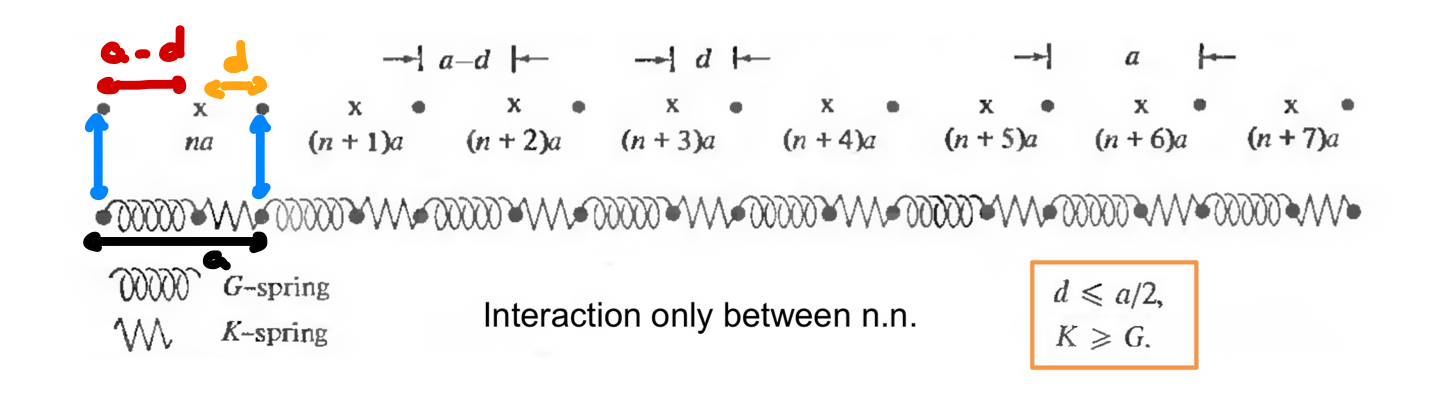
\includegraphics[width=1\textwidth]{images/8-Fononi/Fononi.jpeg}
    \caption{}
\end{figure}

\begin{itemize}
    \item Supponiamo che vi siano due costanti elastiche differenti, denotate da \(G\) e \(K\), e due posizioni di equilibrio differenti: un ione oscilla attorno a \(na\) e l'altro attorno a \(na+d\), con \(d\leq \frac{a}{2}\)
    \item In questo sistema le forze che agiscono tra gli ioni dipendono dalla loro separazione: gli ioni separati da \(d\) interagiscono con una costante elastica \(K\), mentre quelli separati da \(a-d\) interagiscono con una costante \(G\). 
    \item \(K \geq G\), ossia il legame interno (tra ioni in posizione \(na\) e \(na+d\)) è più forte, il che rompe la simmetria del sistema e porta all'esistenza di due branche (acustica e ottica).
\end{itemize}
Definiamo $u_1(na)$ per lo ione che oscilla attorno a $na$, $u_2(na)$ per lo ione che oscilla attorno a $na+d$.\\
L'energia armonica totale del sistema si scrive come:
\begin{equation}
\begin{split}
    U_{\text{arm}} &= \frac{K}{2}\sum_{n} \Bigl[u_1(na) - u_2(na)\Bigr]^2 
    + \frac{G}{2}\sum_{n} \Bigl[u_2(na) - u_1\bigl((n+1)a\bigr)\Bigr]^2.
\end{split}
\end{equation}
Le equazioni del moto per i due ioni si ottengono derivando \(U_{\text{arm}}\) rispetto a \(u_1(na)\) e \(u_2(na)\):
\begin{enumerate}
    \item Per \(u_1(na)\):
    \begin{equation}
    M\,\frac{\partial^2 u_1(na)}{\partial t^2} = -\frac{\partial U}{\partial u_1(na)} = -K\Bigl[u_1(na) - u_2(na)\Bigr] - G\Bigl[u_1(na) - u_2\bigl((n-1)a\bigr)\Bigr].
    \end{equation}
    \item Per \(u_2(na)\):
    \begin{equation}
    M\,\frac{\partial^2 u_2(na)}{\partial t^2} = -\frac{\partial U}{\partial u_2(na)} = -K\Bigl[u_2(na) - u_1(na)\Bigr] - G\Bigl[u_2(na) - u_1\bigl((n+1)a\bigr)\Bigr].
    \end{equation}
\end{enumerate}
Si cerca la soluzione in forma d'onda, ponendo:
\[
u_1(na,t) = \varepsilon_1\, e^{i( kna - \omega t)},\quad
u_2(na,t) = \varepsilon_2\, e^{i( kna - \omega t)}.
\]
Sostituendo queste soluzioni nelle equazioni del moto e dividendo per \(e^{i( kna - \omega t)}\) si ottengono due equazioni algebriche:
\begin{align}
    -M\omega^2\,\varepsilon_1 &= -K\Bigl[\varepsilon_1 - \varepsilon_2\Bigr] - G\Bigl[\varepsilon_1 - \varepsilon_2\,e^{-ika}\Bigr],\\[1mm]
    -M\omega^2\,\varepsilon_2 &= -K\Bigl[\varepsilon_2 - \varepsilon_1\Bigr] - G\Bigl[\varepsilon_2 - \varepsilon_1\,e^{ika}\Bigr].
\end{align}
Riarrangiando:
\begin{align}
    \Bigl[M\omega^2 - (K+G)\Bigr]\varepsilon_1 + \Bigl[K + G\,e^{-ika}\Bigr]\varepsilon_2 &= 0, \\
    \Bigl[K + G\,e^{ika}\Bigr]\varepsilon_1 + \Bigl[M\omega^2 - (K+G)\Bigr]\varepsilon_2 &= 0.
\end{align}
Per avere una soluzione non banale il determinante del sistema deve essere nullo:
\begin{equation}
\begin{split}
    \Bigl[M\omega^2 - (K+G)\Bigr]^2 &- \Bigl[K + G\,e^{-ika}\Bigr]\Bigl[K + G\,e^{ika}\Bigr] = 0.
\end{split}
\end{equation}
Osserviamo che
\[
\Bigl[K + G\,e^{-ika}\Bigr]\Bigl[K + G\,e^{ika}\Bigr] = K^2 + KG\Bigl(e^{ika}+e^{-ika}\Bigr) + G^2,
\]
e poiché
\[
e^{ika}+e^{-ika} = 2\cos(ka),
\]
si ottiene:
\[
\Bigl[M\omega^2 - (K+G)\Bigr]^2 - \Bigl[K^2 + 2KG\cos(ka) + G^2\Bigr] = 0.
\]
Pertanto, l'equazione si scrive:
\[
M^2\omega^4 - 2M\omega^2(K+G) + (K+G)^2 - \Bigl[K^2 + 2KG\cos(ka) + G^2\Bigr] = 0.
\]
Notiamo che
\[
(K+G)^2 - \Bigl[K^2 + 2KG\cos(ka) + G^2\Bigr] = 2KG\bigl[1-\cos(ka)\bigr],
\]
per cui l'equazione diventa:
\[
M^2\omega^4 - 2M\omega^2(K+G) + 2KG\bigl[1-\cos(ka)\bigr] = 0.
\]
Da cui:
\[
\omega^2 = \frac{K+G}{M} \pm \frac{1}{M}\sqrt{K^2 + G^2 + 2KG\cos(ka)}.
\]
Le due soluzioni corrispondono alle due branche:
\begin{itemize}
    \item La \textbf{branca ottica}: per cui le oscillazioni dei due ioni sono in controfase.
    \item La \textbf{branca acustica}: in cui le oscillazioni dei due ioni avvengono in fase.
\end{itemize}
In casi limite si ha:
\begin{enumerate}
    \item Per \(k=0\): si ottengono le soluzioni
    \[
    \omega = 0 \quad \text{(branca acustica)}
    \]
    e
    \[
    \omega = \sqrt{2\frac{K+G}{M}} \quad \text{(branca ottica).}
    \]
    \item Al bordo della prima zona di Brillouin (\(k = \pi/a\)), si ottengono due soluzioni:
    \[
    \omega_1^2 = \frac{K+G}{M} + \frac{K-G}{M} = \frac{2K}{M} \quad \text{(branca ottica)}
    \]
    e
    \[
    \omega_2^2 = \frac{K+G}{M} - \frac{K-G}{M} = \frac{2G}{M} \quad \text{(branca acustica).}
    \]
\end{enumerate}
La relazione tra le due branche è schematizzata nella Figura~\ref{fig:branche}. Nella branca ottica, i due atomi oscillano in controfase, generando dipoli che interagiscono fortemente con la luce (particolarmente importante nei cristalli ionici), mentre nella branca acustica i due atomi oscillano in fase.
\begin{figure} [H]
    \centering
    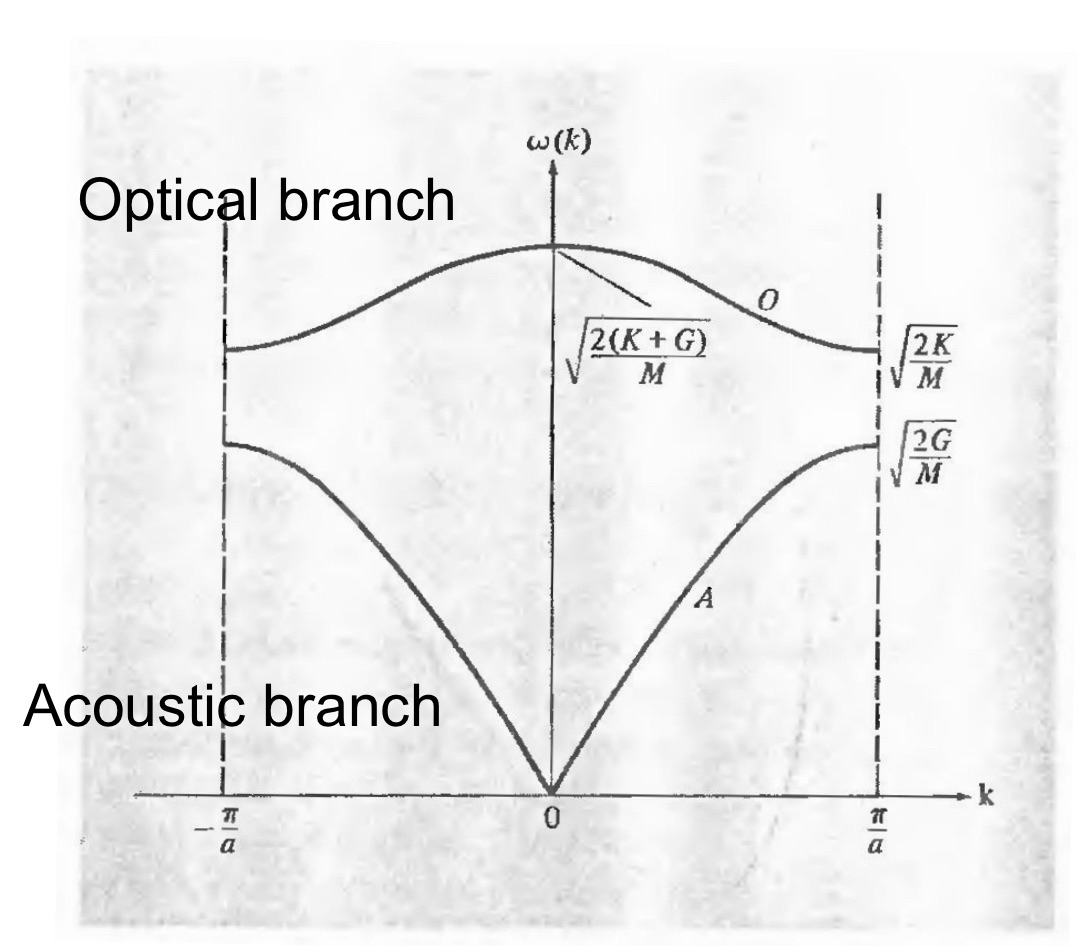
\includegraphics[width=0.7\textwidth]{images/8-Fononi/Branche.jpeg}
    \caption{}
    \label{fig:branche}
\end{figure}

\subsection{Considerazioni Generali}
La trasformata discreta della dynamical matrix, \(\mathbf{D}(\vec{k})\), è un tensore simmetrico e possiede 3 autovettori reali, \(\vec{\varepsilon}_s(\vec{k})\), che corrispondono agli stati normali di vibrazione, dove \(s\) è l'indice di branca. Questi soddisfano:
\begin{equation}
    \mathbf{D}(\vec{k})\,\vec{\varepsilon}_s(\vec{k}) = \lambda_s(\vec{k})\, \vec{\varepsilon}_s(\vec{k}),
\end{equation}
da cui si ricava la relazione di dispersione dei modi normali:
\[
\omega_s(\vec{k}) = \sqrt{\frac{\lambda_s(\vec{k})}{M}}.
\]
Per ogni valore di \(\vec{k}\) in uno spazio tridimensionale, se la cella unitaria contiene \(N\) ioni, ci sono in totale \(3N\) modi normali: in particolare, vi sono 3 branche acustiche (per cui il numero di modi che contribuiscono alla vibrazione traslazionale comune) e \(3(N-1)\) branche ottiche (relative ai movimenti relativi tra gli ioni all'interno della cella).\\
Questi autostati rappresentano, in maniera quantistica, i pacchetti d'onda dei modi normali di vibrazione del solido.



%\section{Misurazione dei fononi}
%Per misurare i fononi c'è bisogno di qualcosa che scatterando con loro ci dia delle informazioni riguardo al loro momento. Utilizzo delle particelle non cariche perché non voglio che ci sia interazione con gli elettroni, dei candidati potrebbero essere quindi i neutroni oppure i fotoni che però sono in un range di energia-momento molto differenti
%\[ \begin{split}
%    &\text{neutroni:} \ \ E_n = \frac{p^2}{2M_n}, \ \ M_n = 1838,65 \ m_e \\
%    &\text{fotoni}: \ \ E_\gamma= pc
%\end{split}\]
%Guardando il grafico in Figura \ref{disp fon} si nota che con i fotoni riesco ad osservare piccoli valori di k quindi sono buoni per controllare la parte centrale della zona di Brillouin poiché è molto vicino a zero, mentre coi neutroni riesco a vedere un'area più grande.
%\begin{figure} [H]
%    \centering
%    
\includegraphics[width=0.5\linewidth]{dispersionefononi.png}
 %   \caption{le linee orizzontali indicano il range energetico dell'energia termica e quindi dei fononi, $E_\gamma$ è l'energia dei fotoni mentre $E_n$ è quella dei neutroni}
 %   \label{disp fon}
%\end{figure} 
%Quindi irraggiando un cristallo con un fascio di neutroni possiamo vedere la perdita (o guadagno) di energia del neutrone che interagisce col cristallo come un fenomeno dovuto all'emissione (o assorbimento) di un fonone e andando a vedere l'angolo di uscita e l'energia dei neutroni uscenti ottengo informazioni sullo spettro fononico. 
%\\~\\
%Considero un neutrone di momento $\mathbf{p}$ ed energia $E = \frac{p^2}{2M_n}$ che in seguito all'urto con un cristallo fuoriesce da esso con momento $\mathbf{p}'$ ed energia $E'=\frac{p'^2}{2M_n}$. \\
%Il neutrone entrando nel solido interagisce con uno o più atomi e causa una vibrazione, quindi in pratica la particella esterna interagisce con un modo normale e scambia un quanto di energia vibrazionale, quel quanto di energia vibrazionale è il fonone. Supponiamo che inizialmente il fonone si trova in uno stato con un numero di occupazione pari a $n_{ks}$ e in seguito all'urto troviamo il cristallo in uno stato nel quale il numero di occupazione dei fononi è $n_{ks}'$, quindi per la conservazione dell'energia abbiamo che:
%\[ \begin{split}
%    &\Delta E = E'-E = -\sum_{ks} \hbar\omega_{ks} \Delta n_{ks} \\
%    & \Delta n_{ks} = n_{ks}'-n_{ks}
%\end{split}\]
%Quindi il cambio dell'energia del neutrone è pari all'energia del fonone che ha assorbito passando attraverso al cristallo meno l'energia del fonone che ha emesso. (s è l'indice della branca). \\
%Invece per quanto riguarda la conservazione del momento, il cambiamento nel momento del neutrone è pari all'inverso del momento cristallino totale del fonone più un vettore del reticolo reciproco
%\[ \Delta p = p' - p = -\sum_{ks} \hbar\mathbf{k} \Delta n_{ks} + \text{vettore reticolo reciproco} \times \hbar\]
%Guardando $\Delta E$ e $\Delta p$ posso ricostruire il grafico in Figura \ref{Branche}. \\
%Ricorda però che il momento cristallino del fonone non è in generale un momento come lo conosciamo. Il "momento cristallino" è semplicemente $\hbar$-volte il vettore d'onda del fonone. Si chiama così perché spesso ha un ruolo simile a quello del momento ma il fatto è che non è soggetto in maniera rigida alla conservazione del momento, la sua simmetria è quella di un reticolo di Bravais e per questo la sua legge di conservazione non è rigida come quella della conservazione del momento ma si conserva sempre più o meno un vettore del reticolo reciproco. \\
%Ora esaminiamo la distribuzione dei nuetroni scatterati emergenti dal cristallo classificando i tipi di scattering che possoo avvenire a seconda del numero totale di fononi con i quali i neutroni scambiano energia passando attraverso al cristallo. 

\section{Misurazione dei Fononi}
Per misurare i fononi all'interno di un cristallo, è necessario utilizzare particelle che possano interagire con essi senza essere significativamente influenzate dagli elettroni. Per questo motivo si prediligono particelle neutre, come i neutroni o i fotoni, che offrono caratteristiche energetiche e di impulso differenti.
\begin{equation}
\begin{split}
&\text{Neutroni:} \quad E_n = \frac{p^2}{2M_n}, \quad M_n = 1838.65\, m_e \\
&\text{Fotoni:} \quad E_\gamma = pc
\end{split}
\end{equation}
Dal confronto tra le relazioni energia-momento si deduce che:
\begin{itemize}
    \item  I fotoni hanno un impulso più piccolo rispetto alla loro energia, rendendoli adatti per esplorare la zona centrale della prima zona di Brillouin, ovvero per bassi valori del vettore d'onda $\mathbf{k}$.
    \item I neutroni, avendo massa e quindi una diversa relazione tra energia e impulso, riescono a coprire una porzione più ampia della zona di Brillouin.
\end{itemize}
\begin{figure}[H]
    \centering
    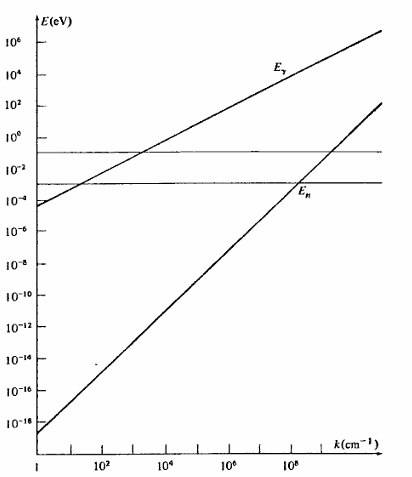
\includegraphics[width=0.5\linewidth]{images/8-Fononi/dispersionefononi.png}
    \caption{Le linee orizzontali rappresentano il range energetico tipico dell'energia termica e quindi dei fononi. $E_\gamma$ rappresenta l'energia dei fotoni, mentre $E_n$ quella dei neutroni.}
    \label{fig:disp-fon}
\end{figure}

L'irraggiamento di un cristallo con un fascio di neutroni permette di analizzare l'interazione tra i neutroni incidenti e i fononi all'interno del reticolo cristallino. Quando un neutrone interagisce con un fonone, può assorbirlo o emetterlo, modificando la propria energia e direzione di moto.\\\\
\textbf{Misurando l'energia e la direzione del neutrone dopo l'interazione, si possono ottenere informazioni sullo spettro fononico del materiale.}\\\\
Consideriamo un neutrone con momento iniziale $\mathbf{p}$ ed energia $E = \frac{p^2}{2M_n}$ che, dopo l'interazione, esce dal cristallo con momento $\mathbf{p}'$ ed energia $E' = \frac{p'^2}{2M_n}$.\\
Durante l'interazione, il neutrone può scambiare energia con i modi vibrazionali del cristallo, ovvero con i fononi. \\
Se inizialmente il fonone si trova in uno stato caratterizzato da un numero di occupazione $n_{\mathbf{k}s}$, al termine dell'interazione tale numero diventa $n_{\mathbf{k}s}'$.\\\\
La variazione di energia del neutrone è quindi data da:
\begin{equation}
\begin{split}
\Delta E &= E' - E = - \sum_{\mathbf{k}s} \hbar \omega_{\mathbf{k}s} (n_{\mathbf{k}s}' - n_{\mathbf{k}s}) \\
         &= - \sum_{\mathbf{k}s} \hbar \omega_{\mathbf{k}s} \Delta n_{\mathbf{k}s}
\end{split}
\end{equation}
Dove $s$ rappresenta l'indice della branca fononica. \textbf{La variazione di energia del neutrone è quindi pari all'energia totale dei fononi emessi meno quella dei fononi assorbiti durante l'interazione.}\\
La conservazione del momento cristallino, invece, implica che:
\begin{equation}
\Delta \mathbf{p} = \mathbf{p}' - \mathbf{p} = - \sum_{\mathbf{k}s} \hbar \mathbf{k} \Delta n_{\mathbf{k}s} + \hbar \mathbf{K}
\end{equation}
Dove $\mathbf{K}$ è un vettore del reticolo reciproco. Questo termine riflette la natura periodica del reticolo cristallino: \textbf{il momento cristallino non si conserva rigidamente come il momento canonico, ma si conserva a meno di $\pm$ un vettore del reticolo reciproco, a causa della simmetria discreta del reticolo di Bravais.\\
Il "momento cristallino" del fonone, definito come $\hbar \mathbf{k}$, non è un vero e proprio momento nel senso classico, ma un'entità legata alla simmetria traslazionale del cristallo.}\\\\
Analizzando la variazione di energia e momento del neutrone in seguito all'interazione, si può ricostruire la relazione di dispersione dei fononi.\\\\

Infine, classificando i neutroni usciti dal cristallo in base alla variazione totale di numero di fononi ($\sum_{\mathbf{k}s} |\Delta n_{\mathbf{k}s}|$), si può distinguere tra:
\begin{itemize}
    \item \textbf{Scattering elastico}: nessun fonone è creato o distrutto ($\Delta n_{\mathbf{k}s} = 0$), l'energia del neutrone resta invariata.
    \item \textbf{Scattering anelastico}: avviene creazione o annichilazione di fononi ($\Delta n_{\mathbf{k}s} \neq 0$), l'energia del neutrone cambia, fornendo informazioni sullo spettro fononico del materiale.
\end{itemize}
Questa tecnica prende il nome di "inelastic neutron scattering" e costituisce uno degli strumenti fondamentali per lo studio delle eccitazioni vibrazionali nei solidi.
\subsection{Zero Phonon Scattering}
In questo caso lo stato finale del cristallo coincide esattamente con quello iniziale, pertanto non viene scambiata energia tra il neutrone e il reticolo. La conservazione del momento cristallino impone che il vettore d'onda del neutrone possa cambiare solo di un multiplo di $\hbar\mathbf{K}$, dove $\mathbf{K}$ è un vettore del reticolo reciproco. Se indichiamo il momento iniziale e finale del neutrone con 
\[
\mathbf{p} = \hbar \mathbf{q} \quad \text{e} \quad \mathbf{p}' = \hbar \mathbf{q}',
\]
i vincoli imposti sono:
\[
\mathbf{q}' = \mathbf{q} \quad \text{oppure} \quad \mathbf{q}' = \mathbf{q} + \mathbf{K}.
\]
Queste condizioni sono le \emph{condizioni di Von Laue} (vedi sezione \ref{subsec:Formulazione-di-Von-Laue}) che, analogamente alla diffrazione di raggi X, determinano i picchi di Bragg. In altre parole, un fascio di neutroni, trattato come un'onda piana con vettore d'onda $\mathbf{q}$, scattera elasticamente solo nelle direzioni che soddisfano queste condizioni. Di conseguenza, tale scattering fornisce informazioni precise sulla struttura cristallina senza coinvolgere processi di eccitazione vibrazionale.

\subsection{One-Phonon Scattering}
Nel caso in cui il neutrone assorbe o emette un singolo fonone, la maggior parte delle informazioni sullo spettro vibrazionale viene trasferita in un unico evento. La conservazione di energia e di momento (tenendo conto del vettore di compensazione del reticolo $\hbar\mathbf{K}$) viene espressa nei seguenti due casi:

\paragraph{Assorbimento di un Fonone}
Il neutrone assorbe un fonone caratterizzato dal vettore d'onda $\mathbf{k}$ e dalla frequenza $\omega_s(\mathbf{k})$, dove $s$ indica la branca fononica. Le relazioni di conservazione sono:
\[
\begin{split}
E' &= E + \hbar \omega_s(\mathbf{k}), \\
\mathbf{p}' &= \mathbf{p} + \hbar \mathbf{k} + \hbar \mathbf{K} = \mathbf{p} + \hbar \left( \mathbf{k} + \mathbf{K} \right).
\end{split}
\]

\paragraph{Emissione di un Fonone}
In questo caso il neutrone emette un fonone e quindi perde un quanto di energia pari a $\hbar \omega_s(\mathbf{k})$. Le condizioni di conservazione diventano:
\[
\begin{split}
E' &= E - \hbar \omega_s(\mathbf{k}), \\
\mathbf{p}' &= \mathbf{p} - \hbar \mathbf{k} + \hbar \mathbf{K} = \mathbf{p} + \hbar \left( \mathbf{K} - \mathbf{k} \right).
\end{split}
\]

Si noti che, dal momento che $\omega_s(\mathbf{k})$ è una funzione periodica nel reticolo reciproco (cioè $\omega_s(\mathbf{k}) = \omega_s(\mathbf{k} \pm \mathbf{K})$), possiamo definire il vettore d'onda del fonone in funzione della variazione di momento del neutrone. Infatti, ignorando esplicitamente il contributo del vettore reticolo $\mathbf{K}$, si ottengono le seguenti relazioni:
\[
\begin{split}
\mathbf{k} &= \frac{\mathbf{p}' - \mathbf{p}}{\hbar} \quad \text{(fonone assorbito)}, \\
\mathbf{k} &= \frac{\mathbf{p} - \mathbf{p}'}{\hbar} \quad \text{(fonone emesso)}.
\end{split}
\]

Pertanto, le equazioni di conservazione dell'energia per i due casi diventano:
\[
\begin{split}
\frac{p'^2}{2M_n} &= \frac{p^2}{2M_n} + \hbar \omega_s\!\left(\frac{p'-p}{\hbar}\right) \quad \text{(fonone assorbito)},\\[1mm]
\frac{p'^2}{2M_n} &= \frac{p^2}{2M_n} - \hbar \omega_s\!\left(\frac{p-p'}{\hbar}\right) \quad \text{(fonone emesso)}.
\end{split}
\]

\subsection{Two-Phonon Scattering}
Nel caso in cui siano coinvolti due fononi, il processo di scattering può avvenire in modalità diverse:
\begin{itemize}
    \item Il neutrone può assorbire o emettere due fononi.
    \item Il neutrone può assorbirne uno e emetterne un altro.
\end{itemize}
In tali casi la combinazione dei vari processi porta a configurazioni multiple che, nonostante trasmettano lo stesso trasferimento totale di energia, contribuiscono a formare uno spettro che tipicamente presenta due componenti:
\begin{enumerate}
    \item Un \textbf{picco intenso} dovuto ai processi one-phonon, che sono molto più probabili.
    \item Un \textbf{background continuo} che rappresenta i contributi dei processi a più di un fonone, visibile ad esempio nella parte indicata dalla freccia in Figura \ref{fig:2phonon-scattering}.
\end{enumerate}
Il picco intenso si deve al fatto che lo scattering che coinvolge un solo fonone ha una probabilità significativamente maggiore rispetto a quello che coinvolge due o più fononi. Di conseguenza, l'analisi del segnale di scattering permette di distinguere chiaramente i contributi elastici (zero phonon), one-phonon e multi-phonon, offrendo informazioni dettagliate sia sulla struttura che sull'interazione vibrazionale del cristallo.

\begin{figure}[H]
    \centering
    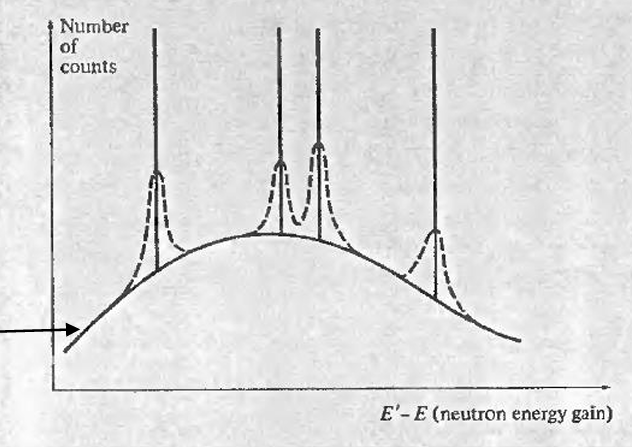
\includegraphics[width=0.7\linewidth]{images/8-Fononi/2phonscatt.png}
    \caption{Spettro di scattering. Il picco intenso corrisponde allo scattering one-phonon, mentre il background continuo evidenzia i processi multi-phonon.}
    \label{fig:2phonon-scattering}
\end{figure}

\section{Conservazione del momento e del momento cristallino}
Dato l'operatore traslazionale $\hat{T}(x) \ket{r} = \ket{r+x}$ l'operatore momento è definito come:
\[ \hat{p} = -i \hbar \left( \vec{\nabla}\hat{T}(x) \right)_{x = 0}\]
considero $\vec{\nabla} T$ come il limite del rapporto incrementale e ho che 
\[ \begin{split}
    & \hat{p_x} = -i\hbar \lim_{a \to 0} \frac{\hat{T}(a\hat{x})-\mathbb{I}}{a} \\
    &(\hat{p}\psi)(r) = -i\hbar \lim_{a \to 0} \frac{(\hat{T}(a)\psi)(r) - \psi(r)}{a} \\
    & = -i\hbar \lim_{a \to 0} \frac{\psi(r-a)-\psi(r)}{a} \\
    & = -i\hbar\frac{\partial}{\partial r} \psi(r)
\end{split}\]
La forma esplicita dell'operatore traslazionale è
\[ \begin{split}
    &\hat{T}(x) = \lim_{N \to \infty} \left( \hat{T} (x/N)\right)^N \\
    &\frac{x}{N} \ \text{è piccolo} \implies \text{espando} \\
    & = \lim_{N \to \infty} \left[ 1-\frac{x}{N}\vec{\nabla} T \right]^N =\\
    & = \lim_{N \to \infty} \left[ 1-\frac{ix\cdot \hat{p}}{N\hbar} \right]^N \\
    & \hat{T}(x) = \exp\left( -\frac{ix\cdot \hat{p}}{\hbar}\right) = 1 - \frac{ix\cdot \hat{p}}{\hbar} - \frac{(x\cdot \hat{p)^2}}{2\hbar^2} + \frac{i(x\cdot \hat{p})^3}{6\hbar^3}+... \\
    & \psi(r-x) = \hat{T}(x)\psi(r) = \exp\left(-  \frac{ix\cdot \hat{p}}{\hbar}\right)\psi(r) = \\
    & = \left( \sum_{n = 0} \frac{1}{n!} \left(  - \frac{i}{\hbar}x \cdot \hat{p}\right)^n\right) \psi(r) = \\
    & = \left( \sum_{n = 0} \frac{1}{n!} \left( -x \cdot\vec{\nabla}\right)^n\right) \psi(r) = \\
    & = \psi(r) - x \cdot \vec{\nabla}\psi(r) + \frac{1}{2!}(x \cdot \vec{\nabla})^2\psi(r)-...
\end{split}\]
La conservazione del momento viene dal fatto che l'hamiltoniana commuta con l'operatore traslazionale:
\[ \begin{split}
    &\left[ \hat{H}, \hat{T}(x) \right] = 0 \\
    & \left[ \hat{H}, 1-\frac{i x \cdot \hat{p}}{N\hbar} \right] = 0 \\
    & \implies \left[ \hat{H}, \hat{p} \right] = 0 \implies \frac{d}{dt}<\hat{p}> = \frac{i}{\hbar}\left[ \hat{H}, \hat{p} \right] = 0
\end{split}\]
In un cristallo la traslazione è data da $\hat{T}(R)$ dove $R$ è un vettore del Bravias lattice
\[ T(R) = e^{ikR} = e^{i(k+K)R}\]
dato che ho $e^{i(k+K)R}$, mi indica che ho un set di vettori siccome $K \in \text{RL}$ quindi p non sarà più ben definito perché ho un insieme di diversi $K$ che mi daranno la stessa traslazione. Quindi è per questo che la conservazione del momento di un cristallo è soddisfatta più o meno un vettore $K$ del reticolo reciproco.


\section{Quantum Harmonic Crystal}
In questo paragrafo calcoliamo il calore specifico a volume costante, \(C_V\), per un solido descritto come un cristallo armonico quantistico. Iniziamo definendo le grandezze macroscopiche fondamentali.
\subsection*{Definizioni Preliminari}
L'energia totale del sistema, dovuta alle vibrazioni quantizzate (fononi), si esprime come:
\begin{equation}
    E_{\text{tot}} = \sum_{n,s} \left(n_s(\mathbf{k}) + \frac{1}{2}\right) \hbar \omega_s(\mathbf{k}),
\end{equation}
dove:
\begin{itemize}
    \item \(n_s(\mathbf{k})\) è il numero di occupazione del fonone nel ramo \(s\) e con vettore d'onda \(\mathbf{k}\);
    \item La presenza del termine \(\frac{1}{2}\) rappresenta l'energia di punto zero, tipica del comportamento quantistico.
\end{itemize}
La distribuzione di Bose-Einstein, che regola la popolazione dei fononi, è data da:
\begin{equation}
    n_s(\mathbf{k}) = \frac{1}{e^{\beta \hbar \omega_s(\mathbf{k})} - 1},
\end{equation}
con \(\beta = \frac{1}{k_B T}\).
L'energia media per unità di volume è:
\begin{equation}
    u(T) = \frac{E_{\text{tot}}}{V},
\end{equation}
e il calore specifico a volume costante è definito come:
\begin{equation}
    C_V = \left(\frac{\partial u(T)}{\partial T}\right)_V.
\end{equation}
Si noti che, in questo contesto, il potenziale chimico \(\mu = 0\) poiché il numero di fononi non è conservato.\\
Riassumendo, possiamo scrivere:
\begin{equation}
    C_V = \frac{1}{V}\sum_{n,s} \frac{\partial}{\partial T} \left[ \hbar \omega_s(\mathbf{k}) \left( \frac{1}{e^{\beta \hbar \omega_s(\mathbf{k})} - 1} + \frac{1}{2} \right) \right].
\end{equation}
\subsection*{Caso Temperature Alte (\(\beta \ll 1\))}
Nel regime delle alte temperature, possiamo espandere la distribuzione di Bose-Einstein per \(x = \beta \hbar \omega\) intorno a \(x=0\). Consideriamo l'espansione:
\begin{equation}
    \frac{1}{e^x - 1} \approx \frac{1}{x + \frac{x^2}{2} + \frac{x^3}{6} + \cdots} \approx \frac{1}{x}\left(1 - \frac{x}{2} + \frac{x^2}{12} + \cdots\right).
\end{equation}
Sostituendo l'espansione nella definizione di \(C_V\) ed esplicitando il termine dell'energia, abbiamo:
\begin{equation}
\begin{split}
    C_V &\approx \frac{1}{V}\sum_{n,s} \frac{\partial}{\partial T} \left[ \hbar \omega_s \left(\frac{k_B T}{\hbar \omega_s} - \frac{1}{2} + \frac{\hbar \omega_s}{k_B T} \cdot \frac{1}{12} \right) \right] \\
    &\approx \frac{1}{V}\sum_{n,s} \left( k_B - \frac{(\hbar \omega_s)^2}{12 k_B} \frac{1}{T^2}\right).
\end{split}
\end{equation}
Dato che, a temperature elevate, ci aspettiamo che il contributo energetico totale sia dominato dal termine costante (secondo il teorema di equipartizione), la somma porta al risultato:
\begin{equation}
    C_V \approx 3R - \frac{1}{V}\sum_{n,s} \frac{(\hbar \omega_s)^2}{12 k_B}\frac{1}{T^2},
\end{equation}
dove \(3R\) rappresenta il contributo classico (in unità di moli, \(R\) è la costante dei gas) e il termine correttivo decresce con \(1/T^2\).

\subsection*{Caso Temperature Basse (\(\beta \gg 1\))}
Nel limite delle basse temperature, i modi vibratori con \(\hbar \omega_s \gg k_B T\) non contribuiscono significativamente all'energia. Inoltre, per basse energie, la relazione di dispersione assume la forma lineare:
\begin{equation}
    \omega_s(\mathbf{k}) \approx c_s\, k,
\end{equation}
con \(c_s\) che rappresenta la velocità del suono nel materiale, e quindi:
\begin{equation}
    x = \beta \hbar c_s k.
\end{equation}
Nel passaggio dal discreto al continuo, la sommatoria si sostituisce con:
\begin{equation}
    \frac{1}{V}\sum_{\mathbf{k}} \to \int \frac{\d\mathbf{k}}{(2\pi)^3}.
\end{equation}
L'energia per unità di volume diventa:
\begin{equation}
\begin{split}
    u(T) &\propto \sum_s \int \frac{\d\mathbf{k}}{(2\pi)^3}\, \hbar \omega_s(\mathbf{k}) \, \frac{1}{e^{\beta \hbar \omega_s(\mathbf{k})} - 1} \\
         &= \sum_s \frac{1}{(2\pi)^3} \cdot 4\pi \int_0^{\infty} \d{k}\, k^2\, \frac{\hbar c_s k}{e^{\beta \hbar c_s k} - 1}.
\end{split}
\end{equation}
Svolgendo il cambio di variabile \(x = \beta \hbar c_s k\), si ottiene:
\begin{equation}
\begin{split}
    u(T) &\propto \sum_s \frac{1}{(2\pi)^3} \cdot 4\pi \int_0^{\infty} \frac{\d{x}}{\beta \hbar c_s}\, \left(\frac{x}{\beta \hbar c_s}\right)^2 \, \frac{\hbar c_s \, \frac{x}{\beta \hbar c_s}}{e^{x} - 1} \\
         &= \sum_s \frac{1}{2\pi^2} \frac{1}{(\beta \hbar c_s)^3} \int_0^{\infty} \frac{x^3}{e^x - 1}\, \d{x}.
\end{split}
\end{equation}
Utilizzando il risultato noto:
\begin{equation}
    \int_0^{\infty} \frac{x^3}{e^x - 1}\, \d{x} = \frac{\pi^4}{15},
\end{equation}
l'energia assume la forma:
\begin{equation}
    u(T) \propto \sum_s \frac{k_B^4}{(\hbar c_s)^3} T^4 \cdot \frac{\pi^4}{15}.
\end{equation}
Il calore specifico a volume costante si ottiene derivando \(u(T)\) rispetto a \(T\):
\begin{equation}
\begin{split}
    C_V &= \frac{\partial u(T)}{\partial T} \propto \sum_s \frac{k_B^4}{(\hbar c_s)^3} \cdot \frac{\pi^4}{15} \cdot 4T^3 \\
    &\propto \frac{2\pi^2}{5}\frac{k_B^4}{(\hbar c_s)^3} T^3.
\end{split}
\end{equation}
Quindi, nel limite delle basse temperature:
\begin{equation}
    C_V \propto T^3,
\end{equation}
in accordo con l'osservazione sperimentale.
\bigskip
\noindent Riassumendo, il comportamento del calore specifico è:
\begin{itemize}
    \item \textbf{A temperature elevate: \(C_V\) tende a un valore costante (con piccole correzioni che decadono come \(1/T^2\)).}
    \item \textbf{A temperature basse: \(C_V \propto T^3\).}
\end{itemize}


\chapter{Nanostrutture}
Il senso di creare una nanostruttura è quello di cambiare le proprietà del materiale confinandolo dimensionalmente e cambiando quindi la sua densità di stati all'energia di Fermi che è ciò che dona le proprietà ad un materiale. 
\begin{figure} [H]
    \centering
    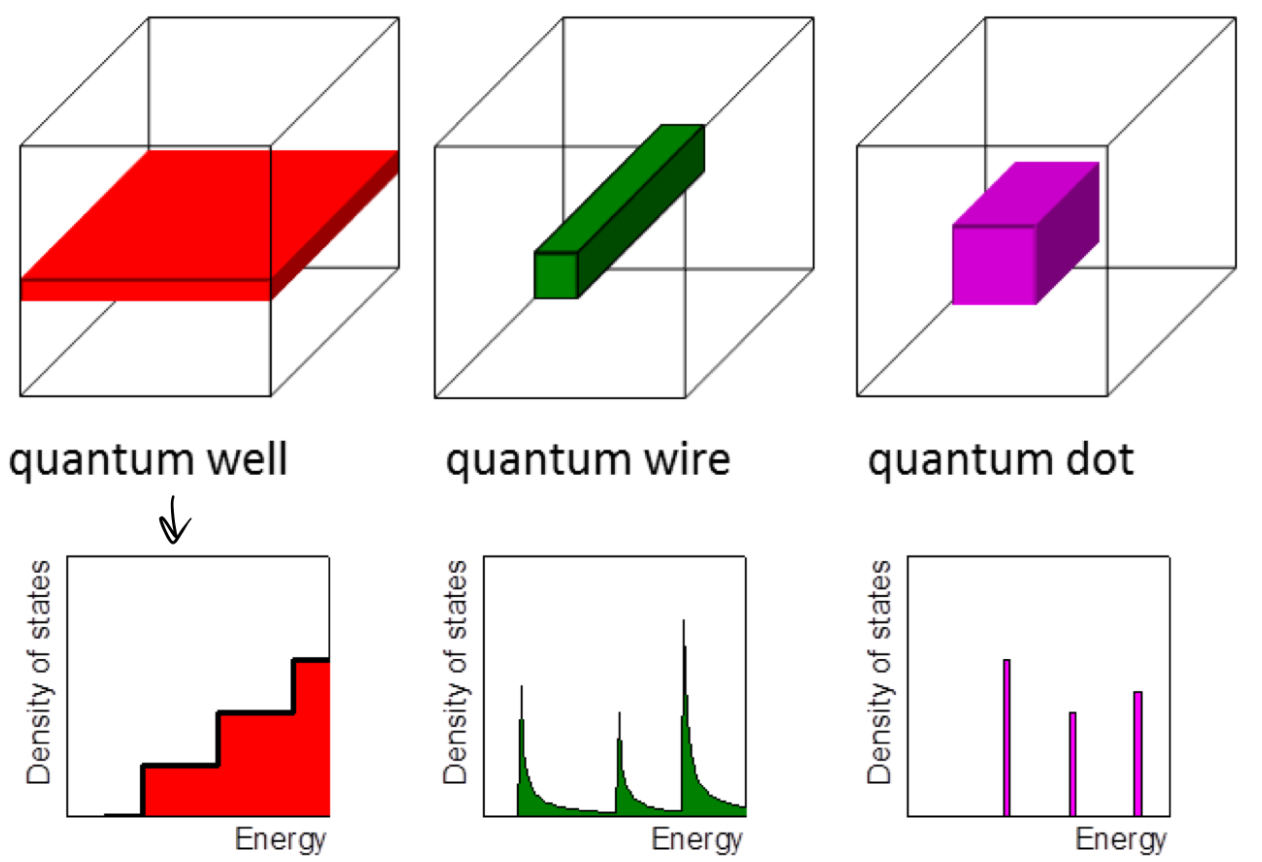
\includegraphics[width=0.5\linewidth]{images/9-Nanostrutture/Nanostr.jpeg}
    \caption{}
    \label{fig:nanostruttura}
\end{figure}

\section{Eterostrutture a confinamento quantico}
Si possono creare delle strutture che combinano un materiale ad alto gap con uno a basso gap, crescendoli su di un substrato layer per layer, creando la struttura in Figura \ref{fig:eterostruttura}
\begin{figure} [H]
    \centering
    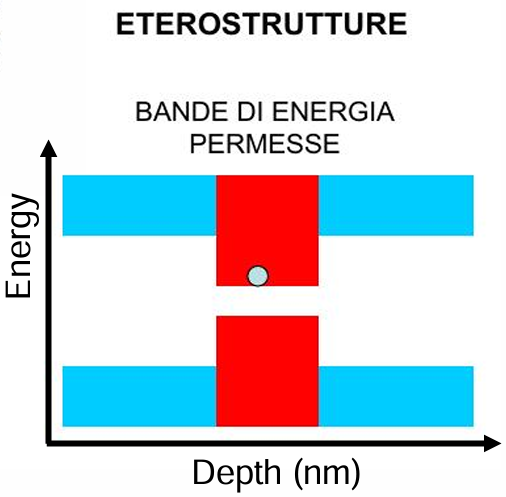
\includegraphics[width=0.4\linewidth]{images/9-Nanostrutture/eterostruttura.png}
    \caption{il materiale azzurro è quello ad alto gap mentre quello rosso è quello a basso gap}
    \label{fig:eterostruttura}
\end{figure} 

L'elettrone non si muove nella zona bianca dell'eterostruttura perché non ho stati permessi
\subsection{Molecular beam epitaxy (MBE)}

La tecnica della \textit{Molecular Beam Epitaxy} (MBE) sfrutta un controllo atomico per la crescita epitassiale di film sottili. Questo documento analizza in maniera dettagliata il processo MBE, focalizzandosi sulla scelta del substrato, l'evaporazione del materiale, il controllo del flusso molecolare e l'importanza delle condizioni in \textit{ultra-alto vuoto} (UHV).

\subsection{Selezione del Substrato}

Il substrato ideale su cui far crescere il film deve essere costituito dallo stesso materiale del film da depositare oppure da un materiale con una costante reticolare simile. Tale compatibilità strutturale è essenziale per:
\begin{itemize}
    \item Minimizzare lo stress reticolare.
    \item Ridurre la formazione di dislocazioni e difetti durante la deposizione.
    \item Favorire una crescita cristallina omogenea e di alta qualità.
\end{itemize}

\subsection{Evaporazione del Materiale}

Il materiale da depositare viene riscaldato all'interno di celle di evaporazione tramite un filamento in tungsteno. L'innalzamento della temperatura induce l'evaporazione del materiale, trasformandolo in un fascio di molecole o atomi.

L'uso del tungsteno, grazie al suo elevato punto di fusione, permette di ottenere:
\begin{itemize}
    \item Una distribuzione stabile ed omogenea dell'energia termica.
    \item Un'evaporazione controllata del materiale.
\end{itemize}

\subsection{Utilizzo dello Shutter}

Prima che il materiale evaporato venga diretto verso il substrato, un \textit{shutter} (otturatore) viene utilizzato per intercettare e controllare il fascio molecolare. In particolare:
\begin{itemize}
    \item Lo shutter permette di bloccare il flusso di molecole fino al momento opportuno.
    \item Una volta aperto, lo shutter consente il passaggio del fascio verso il substrato, garantendo un controllo preciso del tasso di deposizione.
\end{itemize}

\subsection{Ambiente di Ultra-Alto Vuoto (UHV)}

La camera di deposizione è mantenuta in condizioni di ultra-alto vuoto, tipicamente dell'ordine di \(10^{-11}\) mbar, un valore significativamente inferiore rispetto alla pressione atmosferica (circa 1000 mbar). Queste condizioni sono fondamentali per:

\begin{itemize}
    \item \textbf{Prevenzione della contaminazione:} Il vuoto riduce al minimo la presenza di molecole residue che potrebbero contaminare il film sottile.
    \item \textbf{Controllo delle interazioni:} Garantisce che le interazioni tra il fascio molecolare e il substrato avvengano in maniera controllata, evitando reazioni indesiderate.
\end{itemize}

\subsection{Conclusioni}

La MBE rappresenta una tecnica estremamente precisa per la fabbricazione di materiali semiconduttori e sistemi complessi. La combinazione di una selezione accurata del substrato, il controllo termico dell'evaporazione, e l'impiego di uno shutter per regolare il flusso molecolare, consente di ottenere film sottili di alta qualità. Le condizioni in ultra-alto vuoto sono, infine, indispensabili per evitare contaminazioni e assicurare una crescita epitassiale con le proprietà fisiche e strutturali desiderate.
\begin{figure} [H]
    \centering
    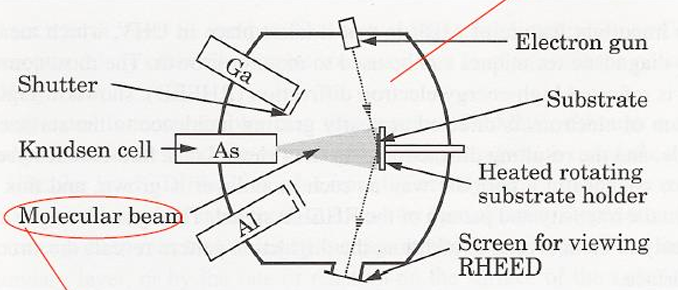
\includegraphics[width=0.8\linewidth]{images/9-Nanostrutture/MBE.png}
    \caption{}
    \label{fig:MBE}
\end{figure} 

\begin{figure} [H]
    \centering
    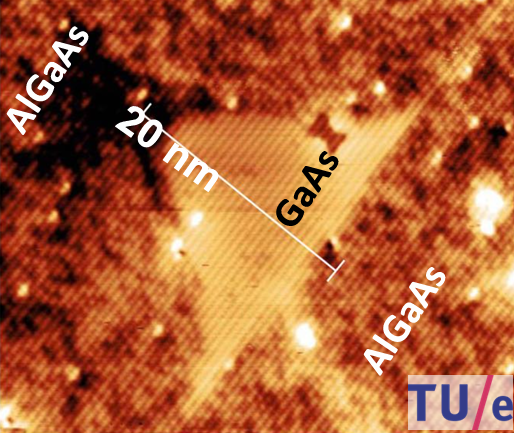
\includegraphics[width=0.5\linewidth]{images/9-Nanostrutture/cross-section.png}
    \caption{l'\ce{AlGaAs} è l'elemento ad alto gap mentre il \ce{GaAs} è quello a basso gap}
    \label{fig:crosss}
\end{figure}

\section{Allineamento delle bande}
Nel progettare eterostrutture a base di semiconduttori, l’obiettivo principale è quello di manipolare i livelli energetici (le bande di conduzione e di valenza) in modo da controllare il comportamento di elettroni e lacune. Ciò si realizza integrando materiali differenti in modo tale che le loro proprietà elettroniche, come il gap di banda e l’affinità elettronica, producano una struttura di bande ingegnerizzata.

\subsection{Regola di Anderson}

Uno degli approcci più utilizzati per stimare l’allineamento delle bande tra due semiconduttori è la \textbf{regola di Anderson}. Secondo questa regola, assumendo che i livelli di energia nel vuoto siano allineati, la differenza tra i livelli della banda di conduzione dei due materiali corrisponde alla differenza nelle loro affinità elettroniche:
\[
\Delta E_c = \chi_1 - \chi_2
\]
dove $\chi$ è l'affinità elettronica. Questa regola fornisce una stima iniziale utile per progettare eterogiunzioni, anche se non tiene conto di effetti interfaccia come stati interfaccia o polarizzazione spontanea.

La scelta della coppia di materiali non deve quindi basarsi solo sulla compatibilità del passo reticolare, ma anche sull’allineamento energetico, in modo da garantire un efficiente trasporto di carica.

\subsection{Effetti del disallineamento reticolare}

È comunque possibile far crescere materiali con un passo reticolare diverso, ma questo genera disallineamenti nella struttura cristallina, con la formazione di difetti strutturali. Tali difetti possono comportare la presenza di zone che intrappolano cariche, note come \textbf{zone morte}.
\\
In alcuni casi, queste zone morte possono risultare utili: introducono livelli energetici intermedi che permettono l’assorbimento di fotoni con energie diverse. \\
Questo principio viene sfruttato per aumentare l’efficienza delle celle fotovoltaiche, consentendo l’assorbimento di una porzione più ampia dello spettro solare.

\subsection{Quantum well}

Una particolare eterostruttura di interesse è la \textbf{quantum well}, ovvero una struttura in cui un materiale a gap minore è confinato tra due materiali a gap maggiore. Questo porta al confinamento quantistico degli elettroni lungo una direzione (solitamente la direzione di crescita epitassiale), lasciando libertà di movimento nelle altre due dimensioni.

Il confinamento quantistico porta alla quantizzazione dei livelli energetici nella banda di conduzione e di valenza. Modificando lo spessore del pozzo quantico, è possibile controllare direttamente l’energia di questi livelli.

\subsection{Esperimenti di fotoluminescenza}

In esperimenti di fotoluminescenza, si irraggia la quantum well con luce avente energia $h\nu > E_{gap}$ del materiale, promuovendo elettroni nella banda di conduzione. Alcuni di questi elettroni vengono confinati negli stati quantizzati del pozzo.

Successivamente, gli elettroni decadono verso la banda di valenza, emettendo fotoni con energia corrispondente alla differenza tra i livelli quantizzati. Controllando la larghezza del pozzo, si controlla anche l’energia dei fotoni emessi, senza dover modificare la composizione chimica del materiale.

\subsection{Conclusioni}

L’ingegnerizzazione delle eterostrutture richiede un’attenta valutazione sia del passo reticolare che dell’allineamento delle bande. Difetti strutturali possono essere sfruttati per aumentare l’assorbimento spettrale, mentre le quantum well offrono un controllo preciso delle proprietà ottiche attraverso la sola variazione geometrica. Questi concetti sono fondamentali per lo sviluppo di dispositivi optoelettronici avanzati come laser a semiconduttore, LED e celle solari multi-giunzione.


\section{Determinare lo stato elettronico}
Supponiamo di trattare la nanostruttura come una perturbazione, per cui avremo:
\begin{equation}
    \begin{split}
        &(H_{id} + V_{per}) \cdot \xi(\vec{r}) = E \cdot \xi(\vec{r})\\
        &H_{id} \cdot \psi_{n,k}= \varepsilon\cdot \psi_{n,k} \hspace{0.4cm}\psi_{n,k}= e^{i\vec{k}\cdot\vec{r}}\cdot u_{n,k}\hspace{0.3cm} \textbf{stati di Bloch} \\
    \end{split}
\end{equation}
Applichiamo la teoria perturbativa per semplicità nel caso 1-D:
\begin{equation}
    \xi(x) = \sum_k \int_{-\frac{\pi}{a}}^{\frac{\pi}{a}} \chi_n(k)\cdot \psi_{n,k}(x)\cdot \frac{\d{k}}{2\pi}y
\end{equation}
\textbf{Prima approssimazione}: banda singola, ossia trascuro i termini al di fuori della banda di conduzione.\\
\textbf{Seconda approssimazione}: consideriamo la perturbazione grande rispetto al passo reticolare $L>>a \implies k$ sta attorno al minimo della banda ossia $k<<\frac{2\pi}{a}$, $k\approx 0$. Ciò implica che le autofunzioni $u_{c,k}$ variano debolmente con $k$, ossia possiamo scrivere:\\
\[\psi_{c,k} = u_{c,k}\cdot e^{ikx} \approx \psi_{c,0} \cdot e^{ikx} \implies \xi(x) \approx \psi_{c,0}(x) \cdot \int_{-\frac{\pi}{a}}^{\frac{\pi}{a}}\chi_c(k) \cdot e^{ikx}\cdot \frac{\d{k}}{2\pi} = \psi_{c,0}\cdot \chi_c(x)\]
        
Dove $\chi_c(x)$ è la trasformata di fourier e prende nome di \textbf{funzione inviluppo} , applichiamo ora la prima parte della Hamiltoniana:
\[H_{id.} \cdot \xi(x) = \int_{-\frac{\pi}{a}}^{\frac{\pi}{a}}\chi_c(k) \cdot H_{id.} \cdot \psi_{c,k}(x)\cdot \frac{\d{k}}{2\pi}  = \int_{-\frac{\pi}{a}}^{\frac{\pi}{a}}\chi_c(k) \cdot \varepsilon_{c,k}\cdot u_{c,k}\cdot e^{ikx}\cdot \frac{\d{k}}{2\pi} \]
\[\approx \psi_{c,0} \int \chi_c(k) \cdot \varepsilon_{c,k} \cdot e^{ikx}\cdot \frac{\d{k}}{2\pi}  \]
Dove gli estremi vanno via in quanto $k\approx 0$
\[\varepsilon_c(k) = \sum_ma_m^c\cdot k^m \approx E_c + \frac{\hbar^2}{2m^*}\cdot k^2 \hspace{0.3cm} \text{con} \hspace{0.3cm} m^* \approx \frac{d^2\varepsilon}{d^2x} \]
\[\implies  E_c \cdot \psi_{c,0} \int \chi_c(k) \cdot e^{ikx}\cdot \frac{\d{k}}{2\pi} + \psi_{c,0} \frac{\hbar^2}{2m^*}\int \chi_c(k) \cdot k^2 \cdot e^{ikx}\cdot \frac{\d{k}}{2\pi}  \]
\[=E_c \cdot \psi_{c,0} \int \chi_c(k) \cdot e^{ikx}\cdot \frac{\d{k}}{2\pi} + \psi_{c,0} \frac{\hbar^2}{2m^*} \cdot \biggr(-\frac{d^2}{d^2x}\cdot \chi_c(x)\biggr)\]
 
Per cui l'equazione agli autovalori $(H_{id}+V_{per.})\cdot \xi = E \cdot \xi$ diventa:\\
\begin{equation}
    \begin{split}
        &\psi_{c,0}(x)\cdot \biggr(E_c-\frac{\hbar^2}{2m^*}\cdot \frac{d^2}{d^2x}\biggr)\cdot \chi_c(x) + V_{per.}\cdot \psi_{c,0}(x) \cdot \chi_c(x) = E \cdot \psi_{c,0}(x) \cdot \chi_c(x)\\
        &\biggr(-\frac{\hbar^2}{2m^*}\cdot \frac{d^2}{d^2x}+V_{per.}\biggr)\cdot \chi_c(x) = (E-E_c)\cdot \chi_c(x)\\
    \end{split}
\end{equation}
\\\\
\textbf{Quindi si ottiene un'equazione di shrodinger sottoposta ad un potenziale perturbativo esterno con autostato la funzione inviluppo $\chi_c(x)$}, osserviamo che non coincide con l'autofunzione del sistema $\xi(x)$, per cui non che deve essere necessariamente una funzione continua con derivata continua.\\\\

\subsection{Esempio: Quantum well a pareti infinite $D=2$}
Supponiamo di avere quindi una buca di potenziale con pareti idealmente infinite $V_0 \to \infty$ tra $-\frac{a}{2}<z<\frac{a}{2}$, le soluzioni avranno la forma:
\begin{equation}
    \begin{split}
        & \phi_n(z) \begin{cases}
            \sqrt{\frac{2}{a}}\cdot \cos\biggr(\frac{n\pi z}{a}\biggr) \hspace{0.3cm} \text{n dispari}\\
            \sqrt{\frac{2}{a}}\cdot \sin\biggr(\frac{n\pi z}{a}\biggr) \hspace{0.3cm} \text{n pari}
        \end{cases}\\
        &\varepsilon_n = \frac{\hbar^2}{2m_e}\cdot \biggr(\frac{n\pi}{a}\biggr)^2\\
    \end{split}
\end{equation}

\subsection{Esempio: Quantum well a pareti finite $(D=2)$}
Per descrivere una Quantum well a pareti finite supponiamo di considerare un sistema in cui l'energia in funzione della coordinata $z$ sia suddivisa in 3 zone: una prima zona che corrisponde ad una energia $V_0$ (barriera), una zona intermedia a energia nulla compresa tra $-\frac{a}{2}< z <\frac{a}{2}$ (fondo della banda di conduzione della quantum well) e una terza zona a energia $V_0$ (barriera).\\
Consideriamo le seguenti ipotesi:\\
\begin{enumerate}
    \item tutte le energia sono misurate dal fondo della quantum well.
    \item la funzione $\psi_{c,0}$ è la stessa per tutte le tre zone con $\xi = \psi_{c,0}\cdot \chi_c(x) $ autostato del sistema.
    \item la massa efficacie $m^*_e$ è la stessa per tutte le tre zone
    \item gli stati a energia $\varepsilon< V_0$ sono \textbf{stati legati} mentre quelli con $\varepsilon> V_0$ sono \textbf{stati delocalizzati}.
\end{enumerate}
\begin{equation}
    \begin{split}
        &\psi_2(z) = C \cdot \begin{cases}
            \cos(kz) \\
            \sin(kz) \end{cases}\hspace{0.3cm}\text{dentro alla quantum well}\\
        &-\frac{\hbar^2}{2m_e}\cdot \frac{d^2}{d^2z}\psi_{1,3}(z)+V_0\cdot\psi_{1,3}(z) = \varepsilon \cdot \psi_{1,3}(z) \hspace{0.3cm}\text{fuori dalla quantum well}\\
        &\psi_1 = D\cdot e^{Kz} \hspace{0.9cm} \psi_3 =D\cdot  e^{-Kz}\hspace{0.9cm}\frac{\hbar^2K^2}{2m_e}= V_0-\varepsilon =B\\
    \end{split}
\end{equation}
Studiamo il caso per $z>\frac{a}{2}$ e per simmetria possiamo dedurre il caso di $z<-\frac{a}{2}$, imponiamo quindi la continuità della funzione e della derivata nel punto di contatto $z=\frac{a}{2}$.\\
\begin{equation}
    \begin{split}
        &\psi\biggr(\frac{a}{2}\biggr)=C\cdot \begin{cases}
            \cos(\frac{ka}{2})\\
            \sin(\frac{ka}{2})\end{cases} = D \cdot e^{-\frac{Ka}{2}}\\
        &\frac{d\psi}{dz}\biggr|_{z=\frac{a}{2}} = C\cdot k \cdot \begin{cases} -\sin(\frac{ka}{2}) \\
        \cos(\frac{ka}{2})  \end{cases} = -D\cdot K\cdot e^{-\frac{Ka}{2}}\\
        &k\cdot \begin{cases}-\tan(\frac{ka}{2})\\ \cot(\frac{ka}{2}) \end{cases}=-K\hspace{0.3cm}\text{dividendo membro a membro le due eq.}\\
        &\begin{cases}\tan(\frac{ka}{2})\\ -\cot(\frac{ka}{2}) \end{cases}= \frac{K}{k} = \frac{1}{k}\cdot \sqrt{\frac{2m_e}{\hbar^2}\cdot (V_0-\varepsilon)}= \sqrt{\frac{2m_eV_0}{\hbar^2k^2}-1}\\    
        &\begin{cases}\tan(\theta)\\ -\cot(\theta) \end{cases}= \sqrt{\frac{2m_eV_0\cdot a^2}{2\hbar^2}\cdot \frac{1}{\theta^2}-1}= \sqrt{\frac{\theta_0^2}{\theta^2}-1}\hspace{0.3cm}\text{definendo}\hspace{0.3cm}\theta= \frac{ka}{2} \hspace{0.3cm}\theta_0^2= \frac{m_eV_0a^2}{2\hbar^2}\\       
    \end{split}
\end{equation}
\\
\begin{figure} [H]
    \centering
    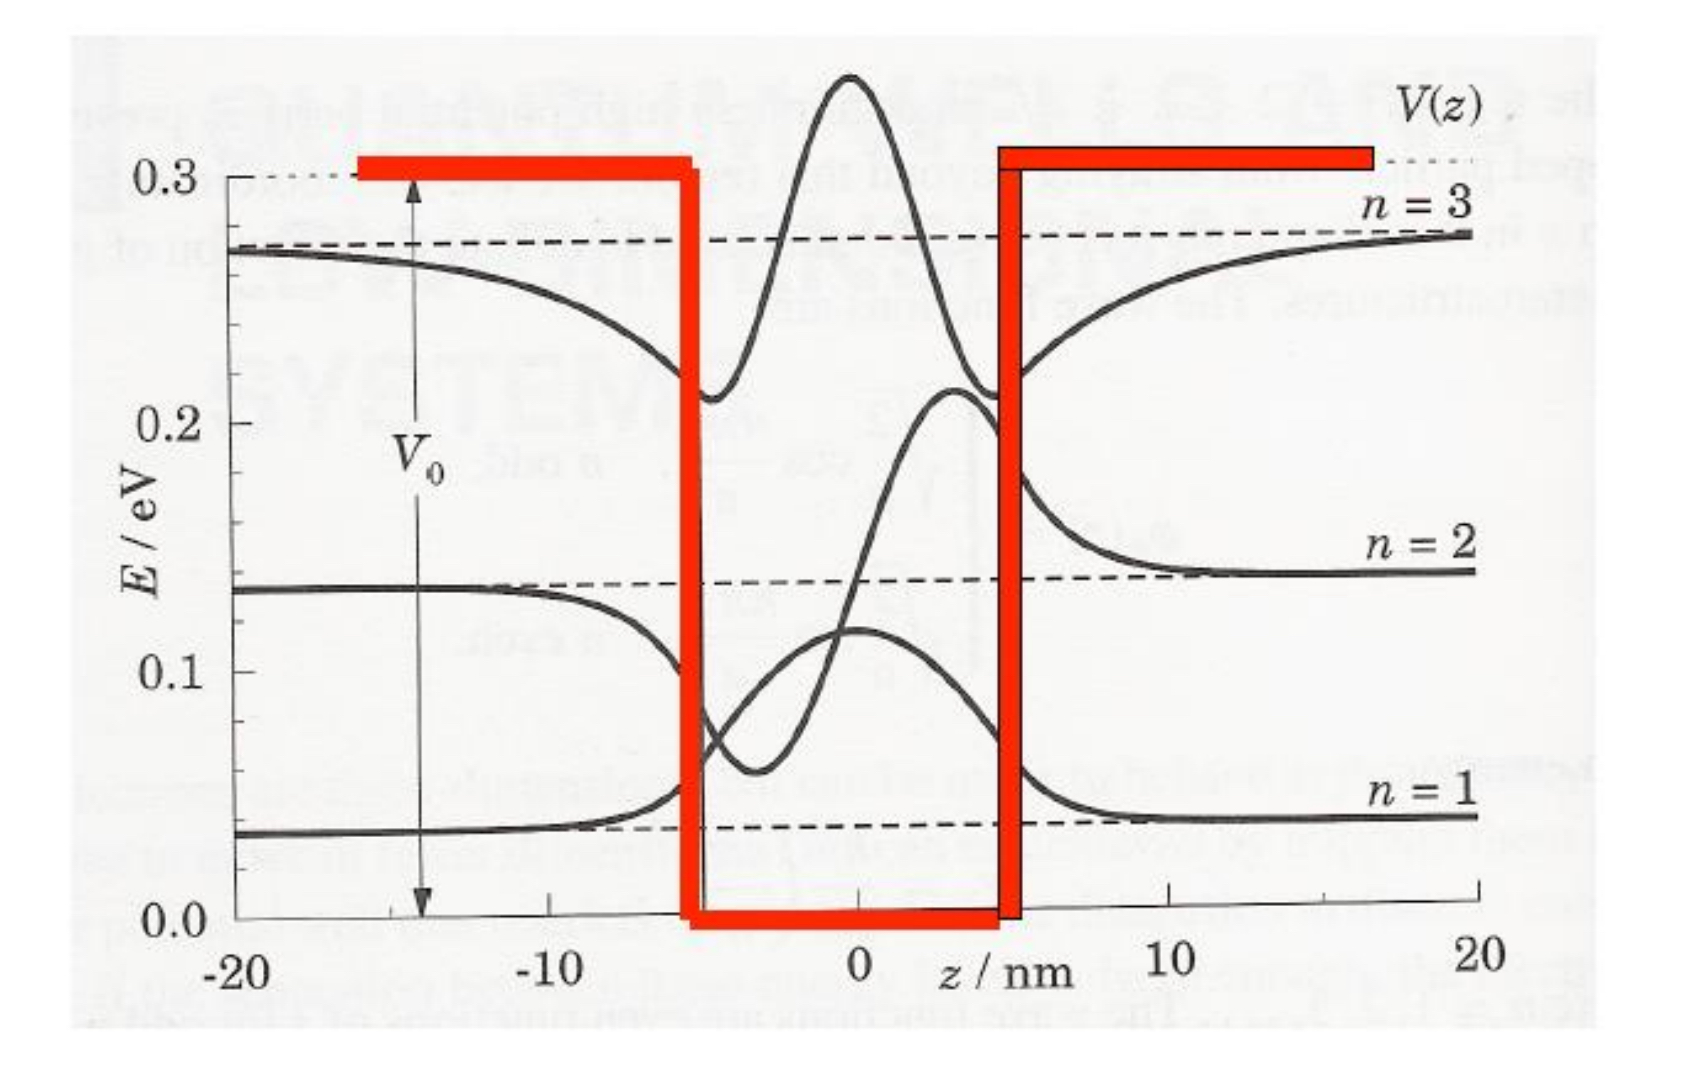
\includegraphics[width=0.7\linewidth]{images/9-Nanostrutture/IMG_1788.jpg}
    \caption{funzioni d'onda risultanti}
\end{figure}
\begin{figure} [H]
    \centering
    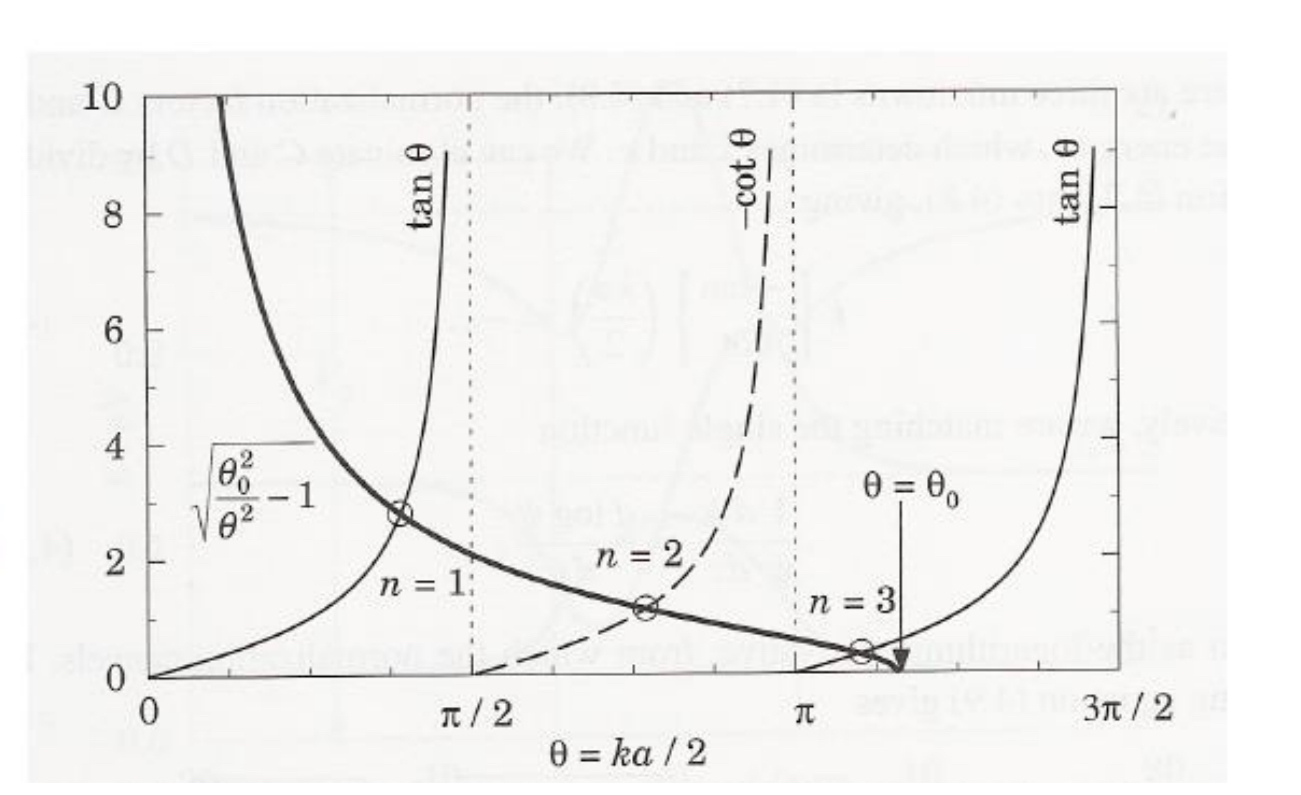
\includegraphics[width=0.7\linewidth]{images/9-Nanostrutture/IMG_1790.jpg}
    \caption{Risoluzione grafica per ricavare $\theta$}
\end{figure}

Considerazioni:
\begin{enumerate}
    \item Il numero di soluzioni dell'equazioni è dato da $\frac{2}{\pi}\cdot \theta_0 = \frac{2}{\pi}\cdot \frac{m_eV_0a^2}{2\hbar^2}$ quindi esiste sempre almeno una soluzione (\textbf{una QW ha sempre uno stato legato}).
    \item Per una QW poco profonda (un solo stato legato) si dimostra che l'energia di legame B dello stato legato è: $B= V_0-\varepsilon \approx \frac{m_eV_0^2a^2}{2\hbar^2}$.
    \item Per un certo stato legato, la probabilità di trovare l'elettrone dentro la QW è: $\int_{-\frac{a}{2}}^\frac{a}{2}|\psi(z)|^2\cdot dz \cdot \bigl[\int_{-\frac{a}{2}}^{\frac{a}{2}}|\psi(z)|^2\cdot dz\bigr]^{-1}$ quindi aumentare la profondità della QW, equivale ad aumentare $\varepsilon$, $B$ e $k$, ossia lo stato è meglio confinato. 
    \item Gli stati a piccolo valore di $n$ sono meno penetranti negli slab di barriera.
\end{enumerate}

\textbf{Il problema completo corrisponde a considerare un'equazione agli autovalori in tre dimensioni in cui la variazione del potenziale avviene solo lungo una direzione $V(x,y,z) =V(z)$}, siccome l'elettrone è libero nel piano $(x,y)$, la soluzione generale avrà la forma: 
\[\psi(x,y,z) = e^{ik_x\cdot x} \cdot e^{ik_y\cdot y}\cdot u(z)\]
sostituendo si ottiene:
\begin{equation}
    \bigl[-\frac{\hbar^2}{2m}\cdot \frac{d^2}{d^2z}+V(z)\bigr]\cdot u(z) = \varepsilon\cdot u(z) \hspace{0.4cm} \varepsilon = E - \frac{\hbar^2k_x^2}{2m}-  \frac{\hbar^2k_y^2}{2m}
\end{equation}
Questa equazione corrisponde a quella che abbiamo risolto sopra per la QW a pareti infinite o finite e conosciamo le soluzioni $u_n(z)$ corrispondenti a stati legati, il sistema è quindi caratterizzato da 3 numeri quantici $k_x,k_y,n$:
\begin{equation}
    \psi_{k_x,k_y,n}(x,y,z) = e^{ik_x\cdot x} \cdot e^{ik_y\cdot y}\cdot u_n(z) \hspace{0.5cm} E_n(k_x,k_y)= \varepsilon_n + \frac{\hbar^2k_x^2}{2m_e} + \frac{\hbar^2k_y^2}{2m_e}
\end{equation}
\begin{figure} [H]
    \centering
    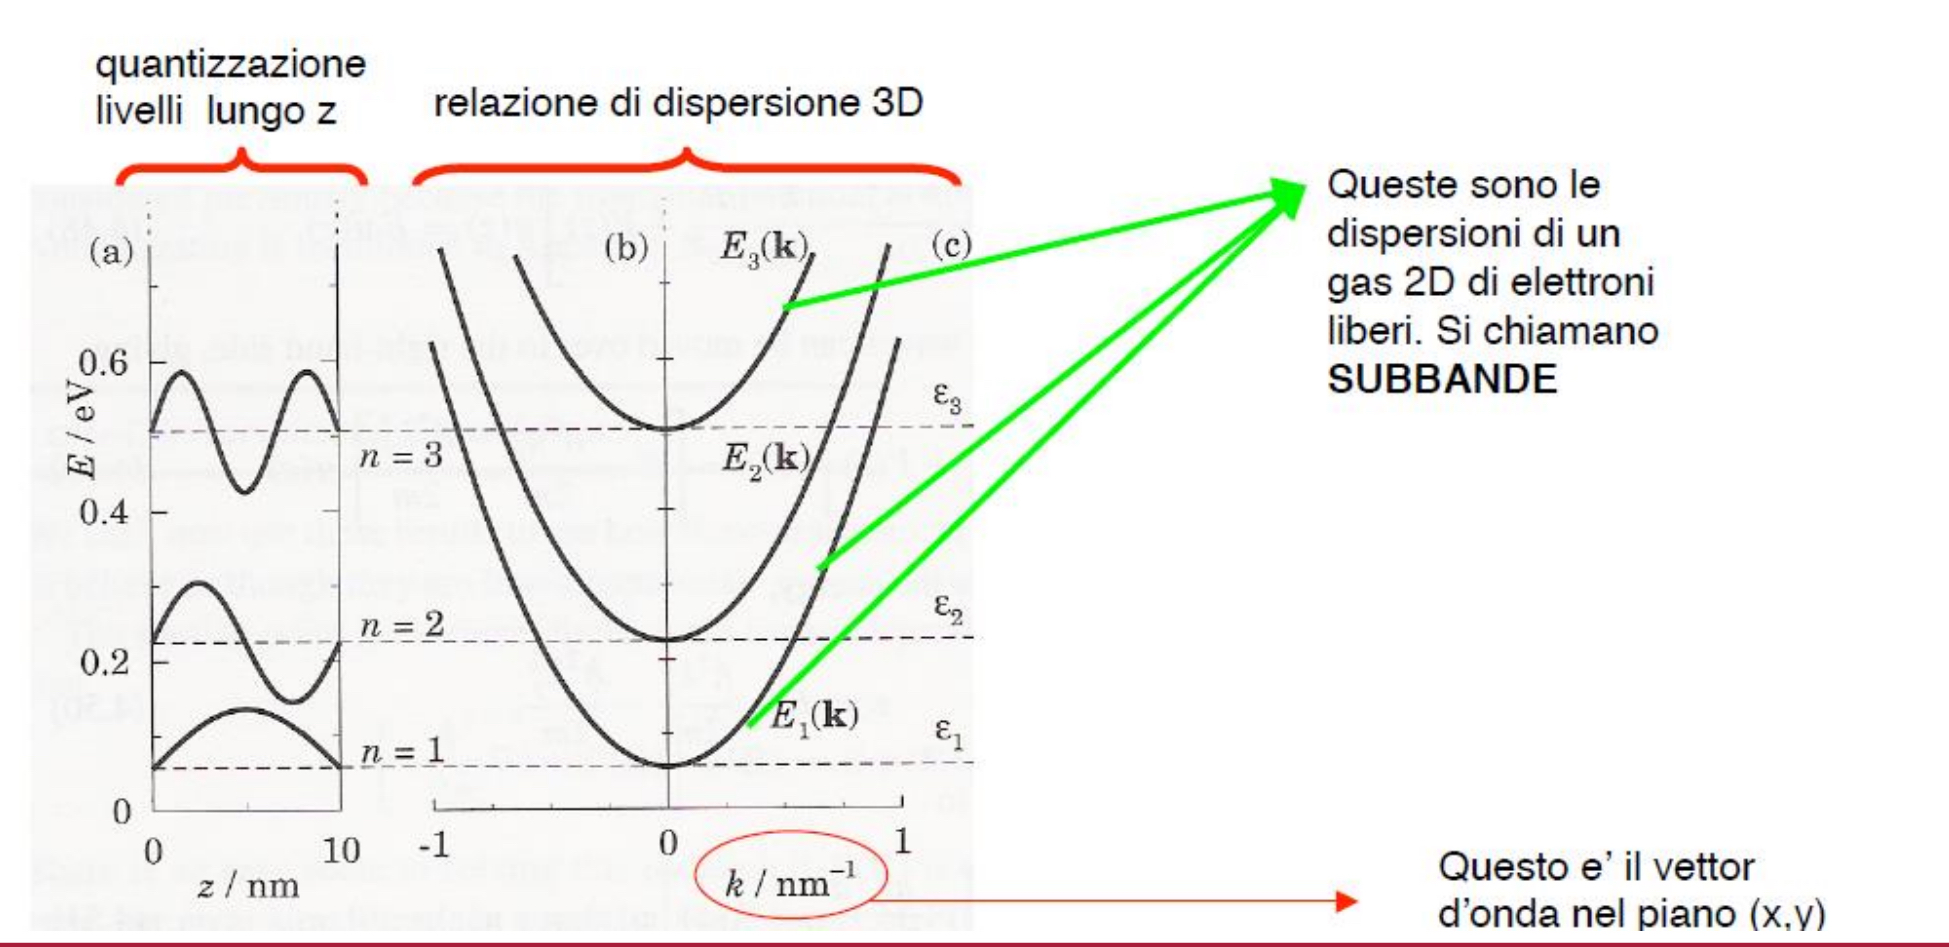
\includegraphics[width=1\linewidth]{images/9-Nanostrutture/IMG_1792.jpg}
\end{figure}
\begin{figure} [H]
    \centering
    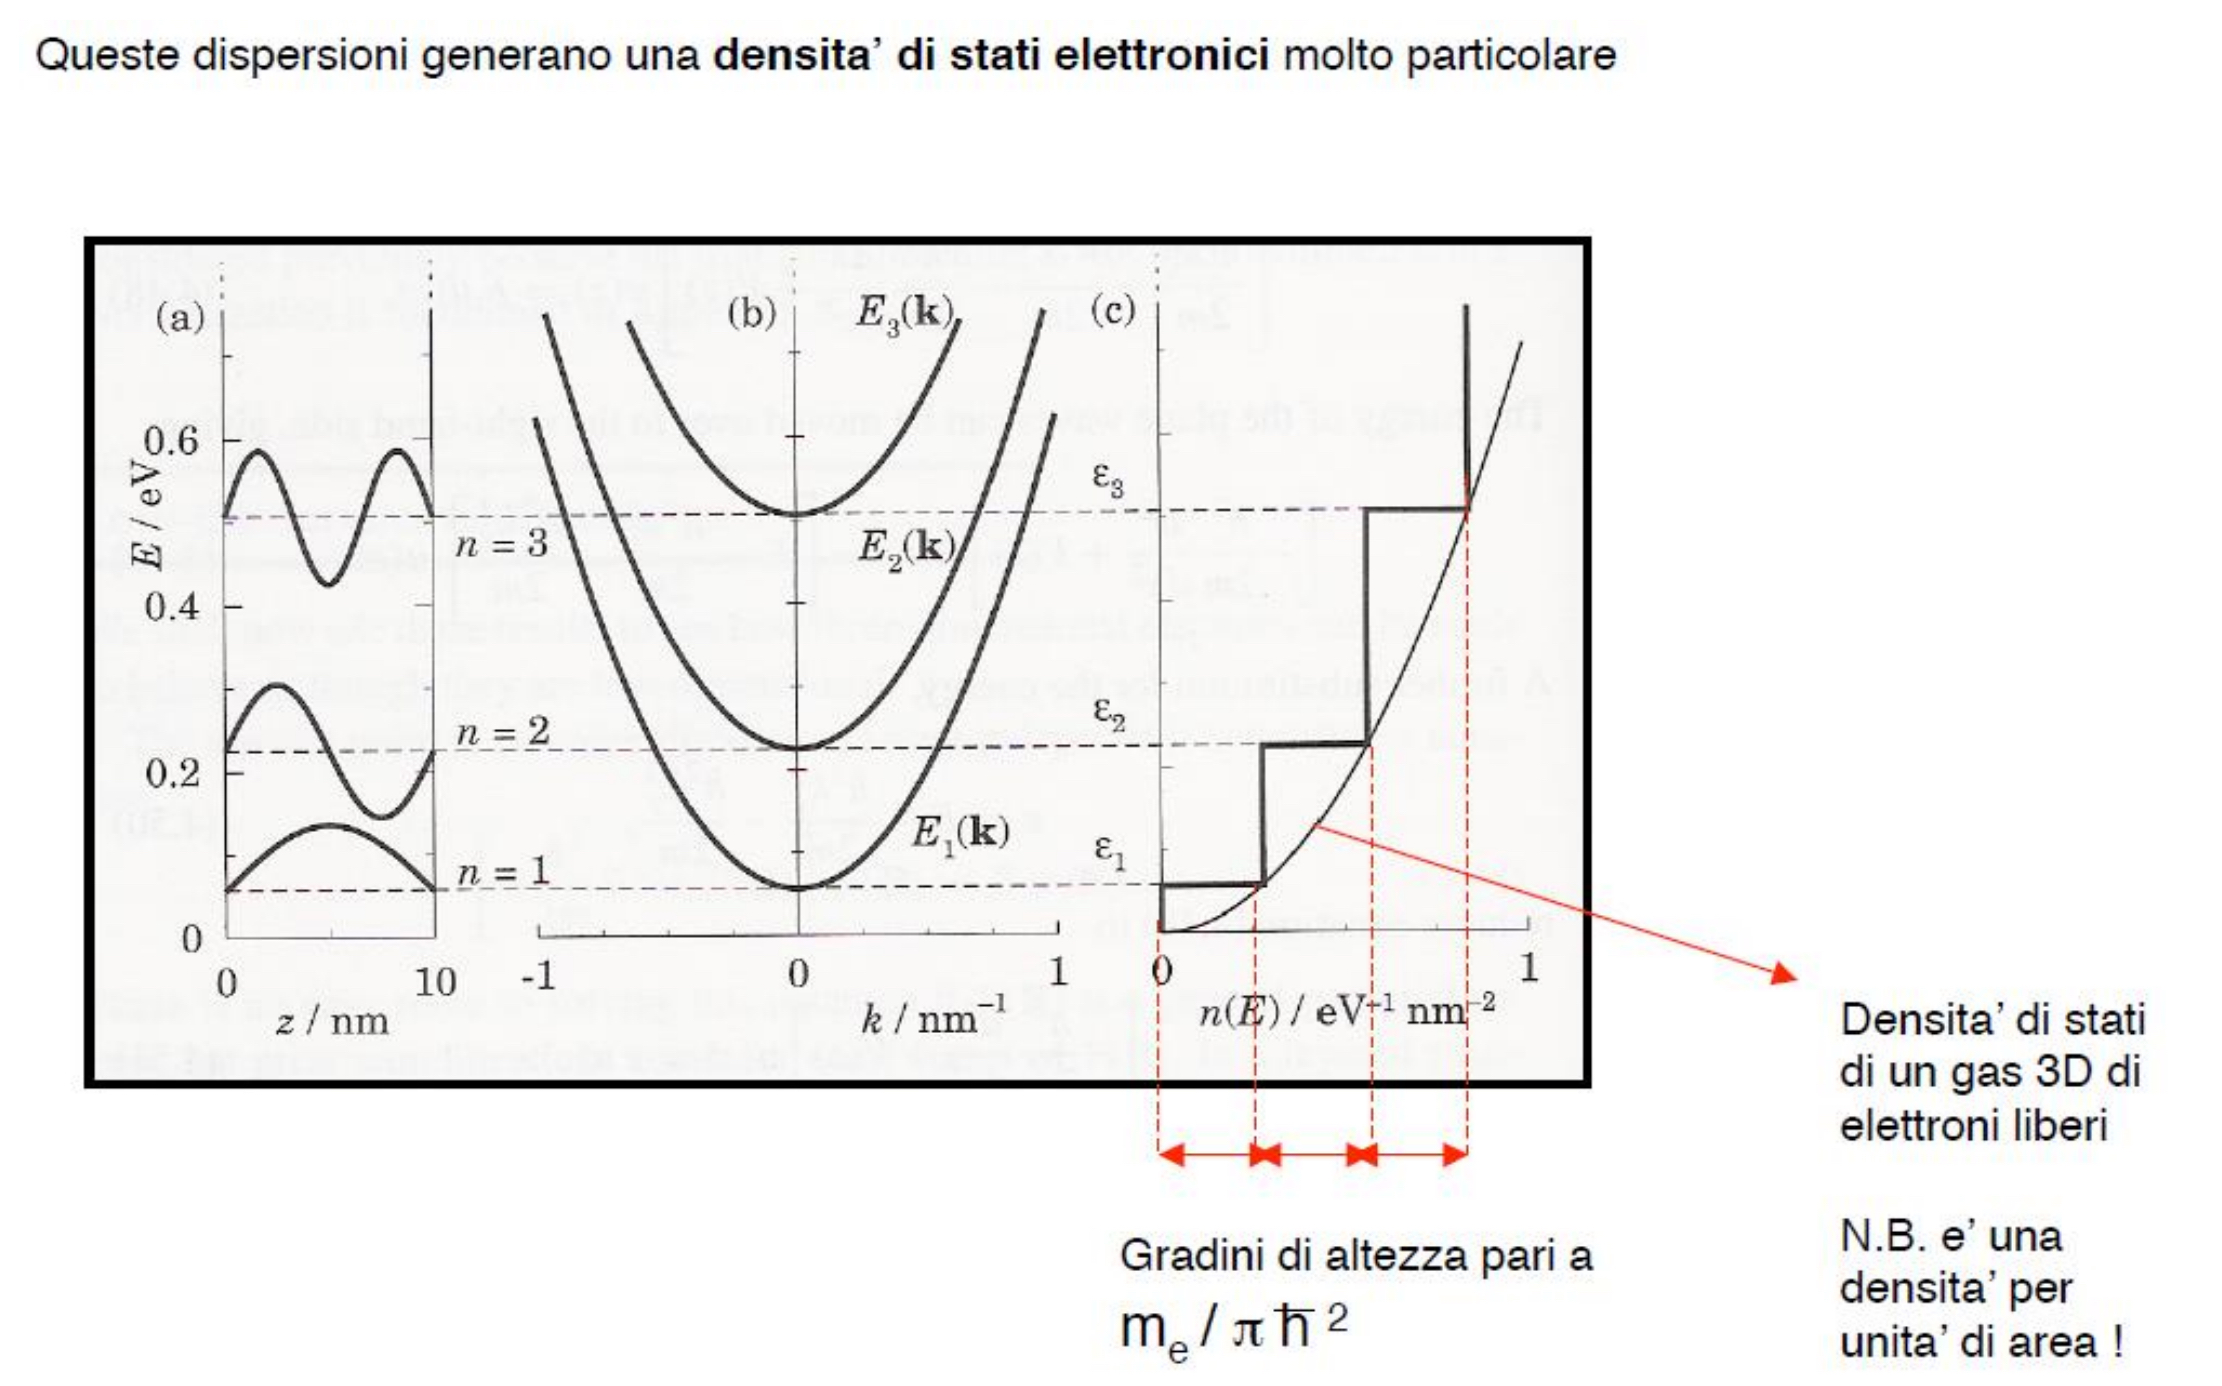
\includegraphics[width=1 \linewidth]{images/9-Nanostrutture/IMG_1793.jpg}
\end{figure}

\section*{Quantum Well a Pareti Finite ($D=2$)}
Si consideri un sistema in cui il potenziale $V(z)$ è suddiviso in tre zone:
\begin{enumerate}
    \item \textbf{Zona 1:} $z < -\frac{a}{2}$ con $V(z) = V_0$ (barriera inferiore);
    \item \textbf{Zona 2:} $-\frac{a}{2} < z < \frac{a}{2}$ con $V(z)=0$ (interno della quantum well, fondo della banda di conduzione);
    \item \textbf{Zona 3:} $z > \frac{a}{2}$ con $V(z) = V_0$ (barriera superiore).
\end{enumerate}
\textbf{Ipotesi:}
\begin{itemize}
    \item Tutte le energie sono misurate rispetto al fondo della quantum well (cioè, $V=0$ nella zona interna).
    \item La massa efficace $m_e^*$ è la stessa in tutte le regioni.
    \item Gli stati con energia $\varepsilon<V_0$ sono \emph{stati legati} (la funzione d'onda decresce esponenzialmente nelle barriere), mentre quelli con $\varepsilon > V_0$ sono \emph{stati delocalizzati}.
\end{itemize}
\subsection*{Soluzione dell'Equazione di Schrödinger}
\subsubsection*{1. Zona Interna della Quantum Well ($-\frac{a}{2} < z < \frac{a}{2}$)}
Nel vano della well il potenziale è nullo e l'equazione stazionaria diventa:
\[
-\frac{\hbar^2}{2m_e}\frac{d^2}{dz^2}\psi_2(z) = \varepsilon\, \psi_2(z).
\]
La soluzione generale è data da:
\[
\psi_2(z)= C\cdot
\begin{cases}
\cos(kz) & \text{(soluzione pari)},\\[1mm]
\sin(kz) & \text{(soluzione dispari)},
\end{cases}
\]
con
\[
k=\sqrt{\frac{2m_e\varepsilon}{\hbar^2}}.
\]

\subsubsection*{2. Zone Esterne (Barriere, $z < -\frac{a}{2}$ e $z > \frac{a}{2}$)}
Per $z$ al di fuori della well il potenziale è costante, $V(z)=V_0$, e l'equazione diventa:
\[
-\frac{\hbar^2}{2m_e}\frac{d^2}{dz^2}\psi_{1,3}(z) + V_0\,\psi_{1,3}(z)= \varepsilon\,\psi_{1,3}(z).
\]
Per stati legati, in cui $\varepsilon<V_0$, si scrive:
\[
-\frac{\hbar^2}{2m_e}\frac{d^2}{dz^2}\psi_{1,3}(z) = (\varepsilon-V_0)\, \psi_{1,3}(z).
\]
Definendo
\[
\frac{\hbar^2K^2}{2m_e} = V_0-\varepsilon \quad \Longrightarrow \quad K=\sqrt{\frac{2m_e(V_0-\varepsilon)}{\hbar^2}},
\]
le soluzioni decrescenti sono:
\[
\psi_1(z)= D\cdot e^{Kz} \quad (z< -\tfrac{a}{2}), \quad \psi_3(z)= D\cdot e^{-Kz}\quad (z>\tfrac{a}{2}).
\]

\subsection*{Condizioni al Contorno}
Per garantire la regolarità della soluzione si impongono la continuità della funzione d'onda e della sua derivata nei punti di confine $z=\pm \frac{a}{2}$. Consideriamo il caso $z=\frac{a}{2}$ (il caso $z=-\frac{a}{2}$ segue per simmetria).

\subsubsection*{Continuità della Funzione}
Si ha:
\[
\psi_2\Bigl(\frac{a}{2}\Bigr)= \psi_3\Bigl(\frac{a}{2}\Bigr),
\]
da cui:
\[
C\cdot
\begin{cases}
\cos\left(\frac{ka}{2}\right) & \text{(soluzione pari)},\\[1mm]
\sin\left(\frac{ka}{2}\right) & \text{(soluzione dispari)}
\end{cases}
= D\cdot e^{-K\frac{a}{2}}.
\]
\subsubsection*{Continuità della Derivata}
Si richiede:
\[
\frac{d\psi}{dz}\Big|_{z=\frac{a}{2}^-} = \frac{d\psi}{dz}\Big|_{z=\frac{a}{2}^+}.
\]
Per la regione interna (zona 2) si ha:
\[
\frac{d\psi_2}{dz}\Big|_{z=\frac{a}{2}} = C\cdot k\cdot
\begin{cases}
-\sin\left(\frac{ka}{2}\right) & \text{(soluzione pari)},\\[1mm]
\cos\left(\frac{ka}{2}\right) & \text{(soluzione dispari)},
\end{cases}
\]
mentre per la zona esterna (zona 3), derivando l'esponenziale, si ottiene:
\[
\frac{d\psi_3}{dz}\Big|_{z=\frac{a}{2}} = -D\cdot K\cdot e^{-K\frac{a}{2}}.
\]

\subsubsection*{Equazioni di Quantizzazione}

Dividendo l'equazione della derivata per quella della funzione (in modo da eliminare le costanti $C$ e $D\cdot e^{-K\frac{a}{2}}$) si ottengono due casi:
\paragraph{Soluzione Pari}
\[
\frac{-C\,k\,\sin\left(\frac{ka}{2}\right)}{C\,\cos\left(\frac{ka}{2}\right)} = -K \quad \Longrightarrow \quad k\, \tan\left(\frac{ka}{2}\right)= K.
\]
\paragraph{Soluzione Dispari}
\[
\frac{C\,k\,\cos\left(\frac{ka}{2}\right)}{C\,\sin\left(\frac{ka}{2}\right)} = -K \quad \Longrightarrow \quad -k\,\cot\left(\frac{ka}{2}\right)= K.
\]
Definendo l'angolo adimensionale
\[
\theta = \frac{ka}{2},
\]
le condizioni diventano:
\[
\begin{cases}
\tan(\theta)=\dfrac{K}{k} & \text{(stato pari)}, \\[2mm]
-\cot(\theta)=\dfrac{K}{k} & \text{(stato dispari)}.
\end{cases}
\]
Notiamo che, essendo
\[
k=\sqrt{\frac{2m_e\varepsilon}{\hbar^2}} \quad \text{e} \quad K=\sqrt{\frac{2m_e(V_0-\varepsilon)}{\hbar^2}},
\]
possiamo scrivere:
\[
\frac{K}{k} = \sqrt{\frac{V_0-\varepsilon}{\varepsilon}}.
\]
Introducendo il parametro adimensionale
\[
\theta_0^2=\frac{m_eV_0a^2}{2\hbar^2},
\]
si ottiene:
\[
\frac{K}{k} = \sqrt{\frac{\theta_0^2}{\theta^2} -1}.
\]
Le equazioni trascendenti risultanti sono:
\[
\begin{cases}
\tan(\theta)=\sqrt{\dfrac{\theta_0^2}{\theta^2}-1} & \text{(stato pari)}, \\[2mm]
-\cot(\theta)=\sqrt{\dfrac{\theta_0^2}{\theta^2}-1} & \text{(stato dispari)}.
\end{cases}
\]
\begin{figure}[h]
\centering
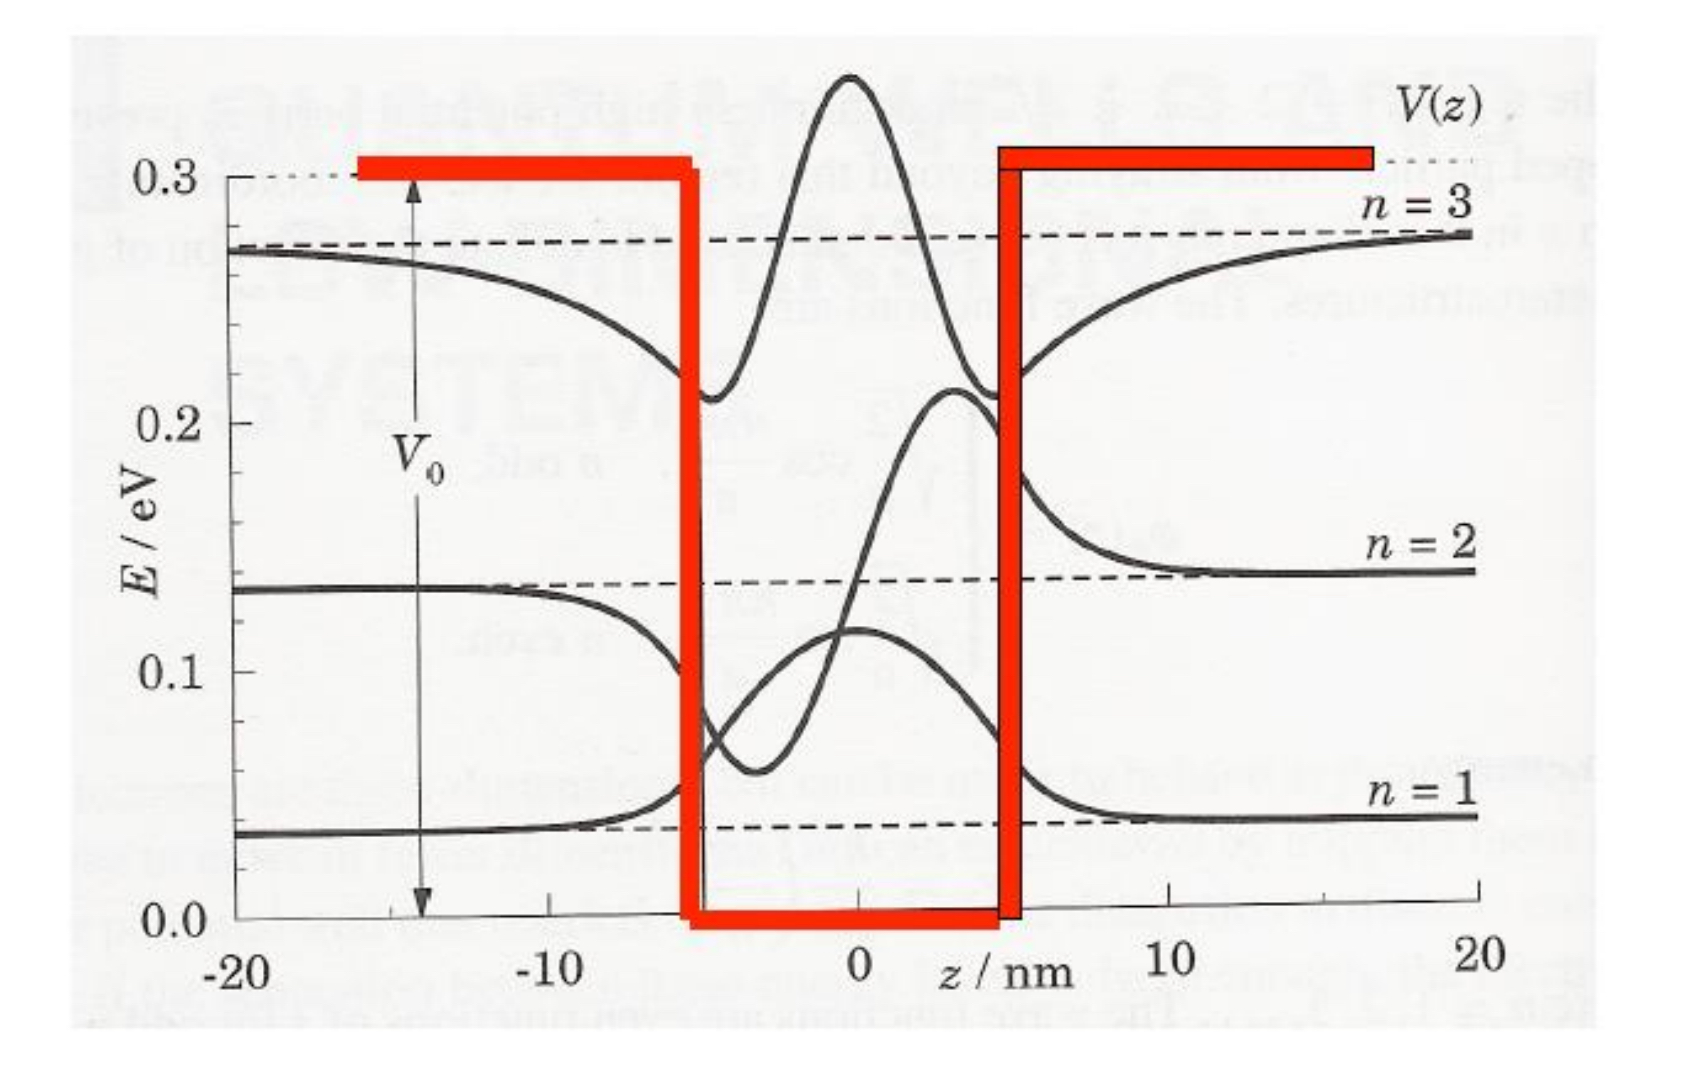
\includegraphics[width=0.7\linewidth]{images/9-Nanostrutture/IMG_1788.jpg}
\caption{Andamento della funzione d'onda all'interno e all'esterno della QW.}
\end{figure}

\begin{figure}[h]
\centering
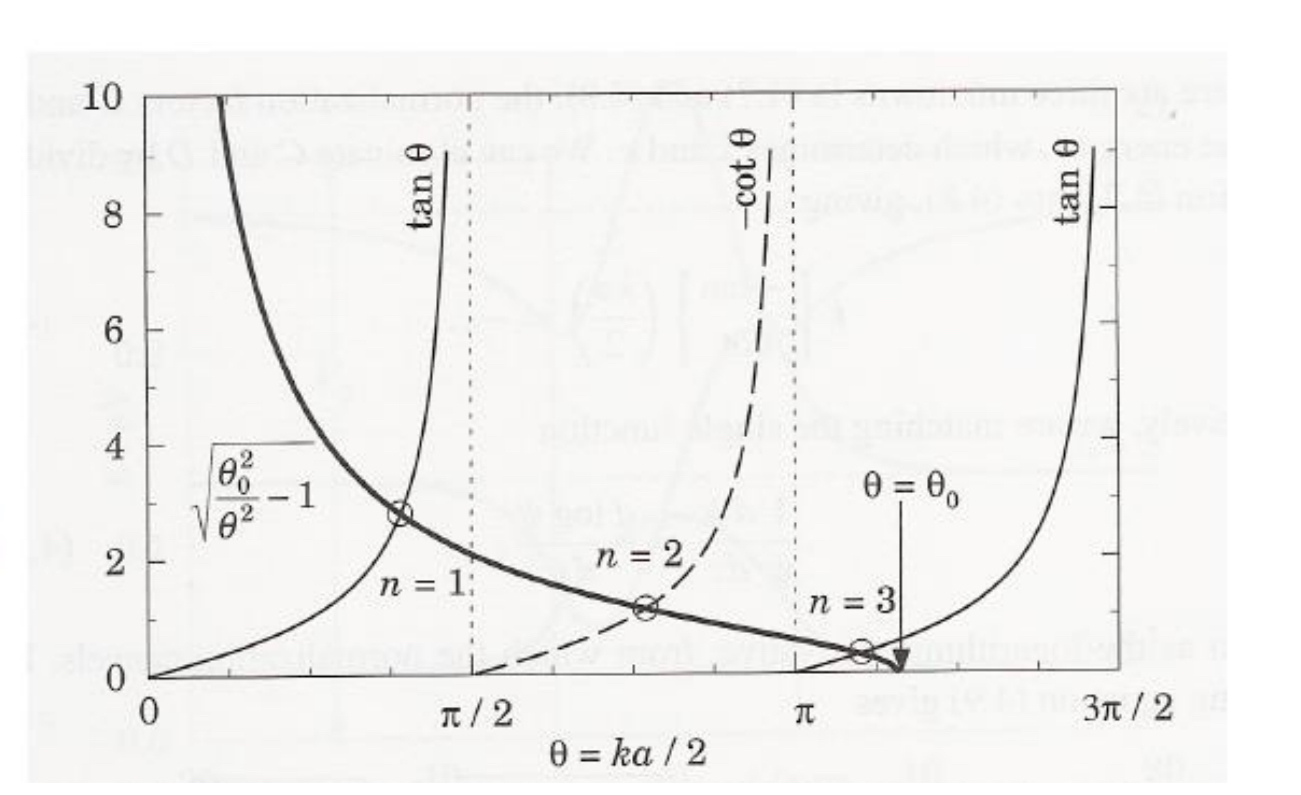
\includegraphics[width=0.7\linewidth]{images/9-Nanostrutture/IMG_1790.jpg}
\caption{Risoluzione grafica per determinare $\theta$.}
\end{figure}

\subsection*{Interpretazione dei Risultati}
\begin{enumerate}
    \item \textbf{Numero di Soluzioni:} \\
    L'equazione trascendente mostra che il numero di soluzioni (stati legati) è approssimativamente:
    \[
    N \approx \frac{2\theta_0}{\pi} = \frac{2}{\pi}\sqrt{\frac{m_eV_0a^2}{2\hbar^2}},
    \]
    garantendo almeno una soluzione, ossia, una quantum well ha sempre almeno uno stato legato.
    
    \item \textbf{Quantum Well Poco Profonda:} \\
    Nel caso in cui vi sia un solo stato legato, il legame energetico, definito da
    \[
    B = V_0 - \varepsilon,
    \]
    risulta approssimativamente:
    \[
    B \approx \frac{m_eV_0^2a^2}{2\hbar^2}.
    \]
    
    \item \textbf{Confinamento:} \\
    La probabilità di trovare l'elettrone all'interno della well è data da:
    \[
    P = \frac{\displaystyle \int_{-\frac{a}{2}}^{\frac{a}{2}} |\psi(z)|^2\,dz}{\displaystyle \int_{-\infty}^{+\infty} |\psi(z)|^2\,dz}.
    \]
    L'aumento di $V_0$ porta a un aumento di $\varepsilon$, $B$ e $k$, e dunque il confinamento nella quantum well diventa migliore.
    
    \item \textbf{Penetrazione nelle Barriere:} \\
    Gli stati a bassi valori di $n$ presentano minore penetrazione nelle regioni delle barriere, in quanto il parametro $K$ risulta maggiore, facendo decadere più rapidamente la funzione esponenziale nelle regioni $z < -\frac{a}{2}$ e $z > \frac{a}{2}$.
\end{enumerate}
\subsection*{Estensione a Tre Dimensioni}
\begin{figure} [H]
    \centering
    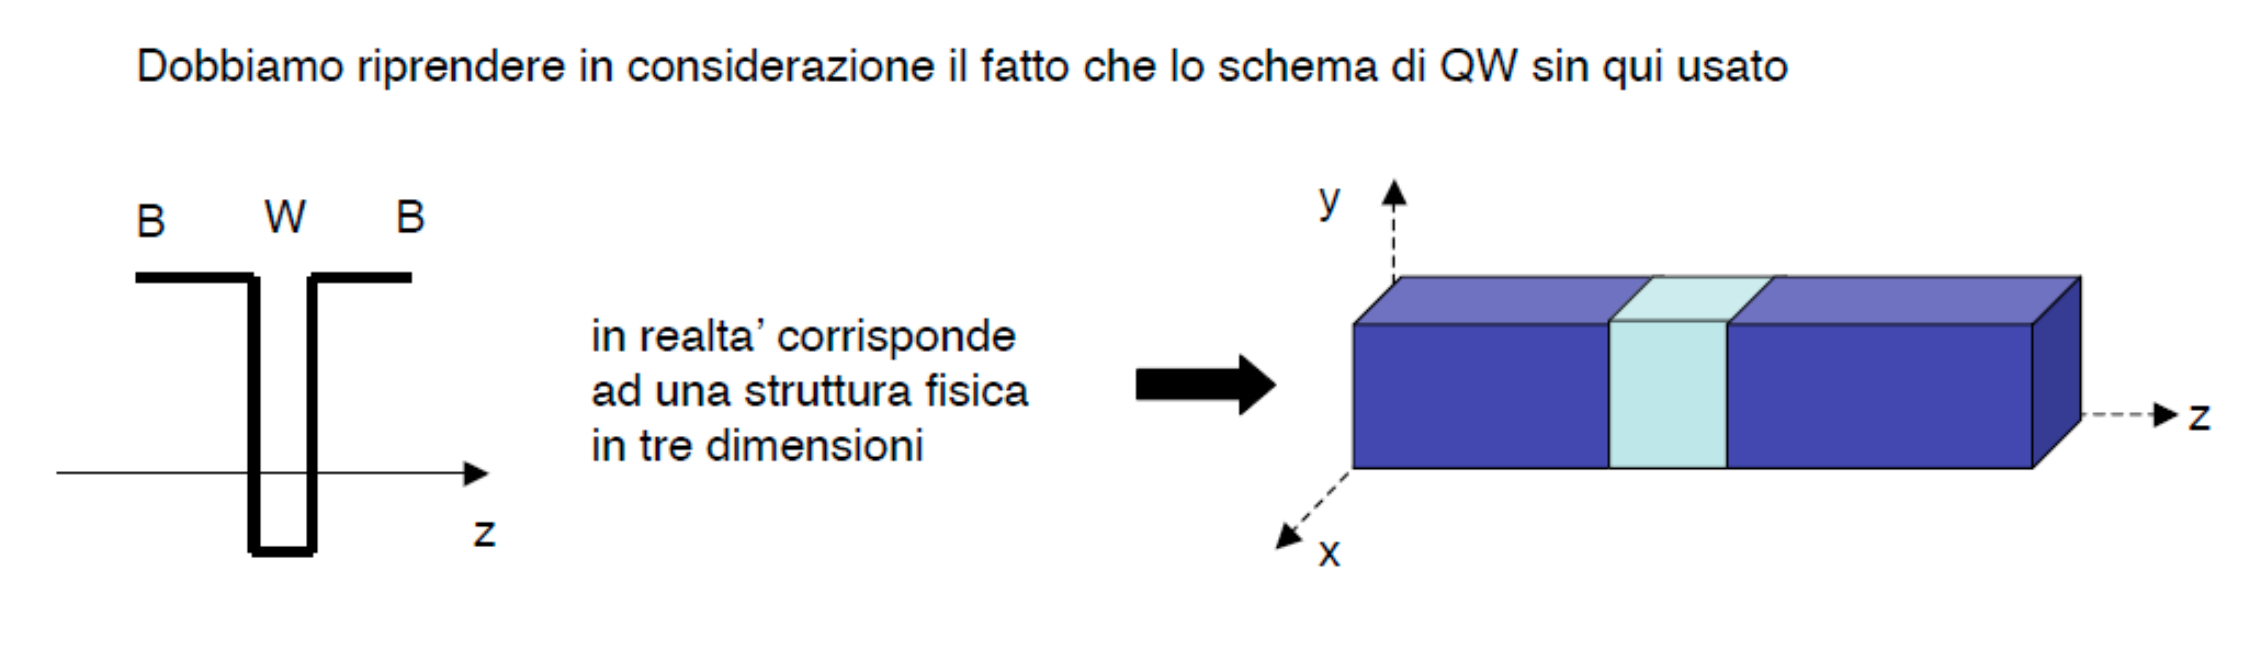
\includegraphics[width=1.1\linewidth]{images/9-Nanostrutture/IMG_1791.jpg}
\end{figure}

\textbf{Il problema completo corrisponde a considerare un'equazione agli autovalori in tre dimensioni in cui la variazione del potenziale avviene solo lungo una direzione $V(x,y,z) =V(z)$}, siccome l'elettrone è libero nel piano $(x,y)$, la soluzione generale avrà la forma: 
\[\psi(x,y,z) = e^{ik_x\cdot x} \cdot e^{ik_y\cdot y}\cdot u(z)\]
dove $u(z)$ soddisfa l'equazione unidimensionale:
\[
\left[-\frac{\hbar^2}{2m_e}\frac{d^2}{dz^2}+V(z)\right] u(z)= \varepsilon\, u(z),
\]
con
\[
\varepsilon = E - \frac{\hbar^2k_x^2}{2m_e} - \frac{\hbar^2k_y^2}{2m_e}.
\]
Gli autostati di $u(z)$ sono quelli determinati precedentemente, etichettati da un indice quantico $n$. L'energia totale dell'elettrone assume quindi la forma:
\[
E_n(k_x,k_y)= \varepsilon_n + \frac{\hbar^2}{2m_e}(k_x^2+k_y^2),
\]
e la funzione d'onda completa si scrive:
\[
\psi_{k_x,k_y,n}(x,y,z)= e^{ik_xx}\, e^{ik_yy}\, u_n(z).
\]
\begin{figure}[h]
\centering
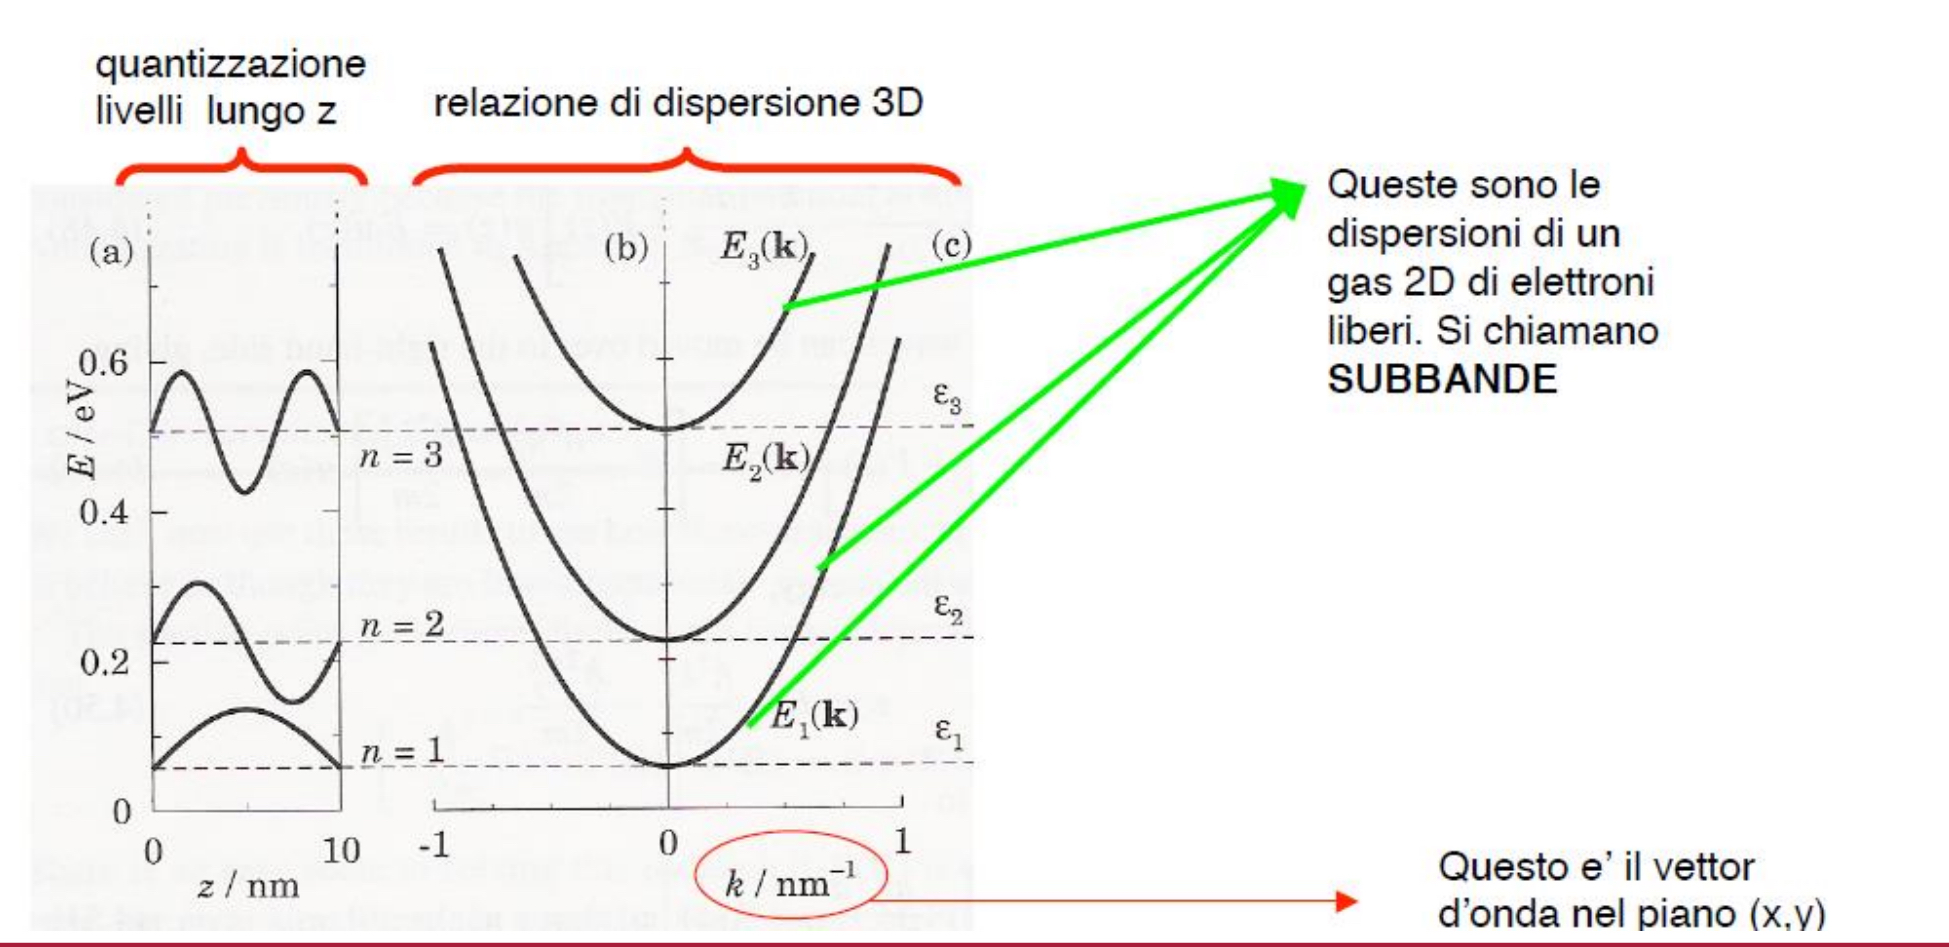
\includegraphics[width=\linewidth]{images/9-Nanostrutture/IMG_1792.jpg}
\caption{Profili delle funzioni d'onda estese.}
\end{figure}

\begin{figure}[h]
\centering
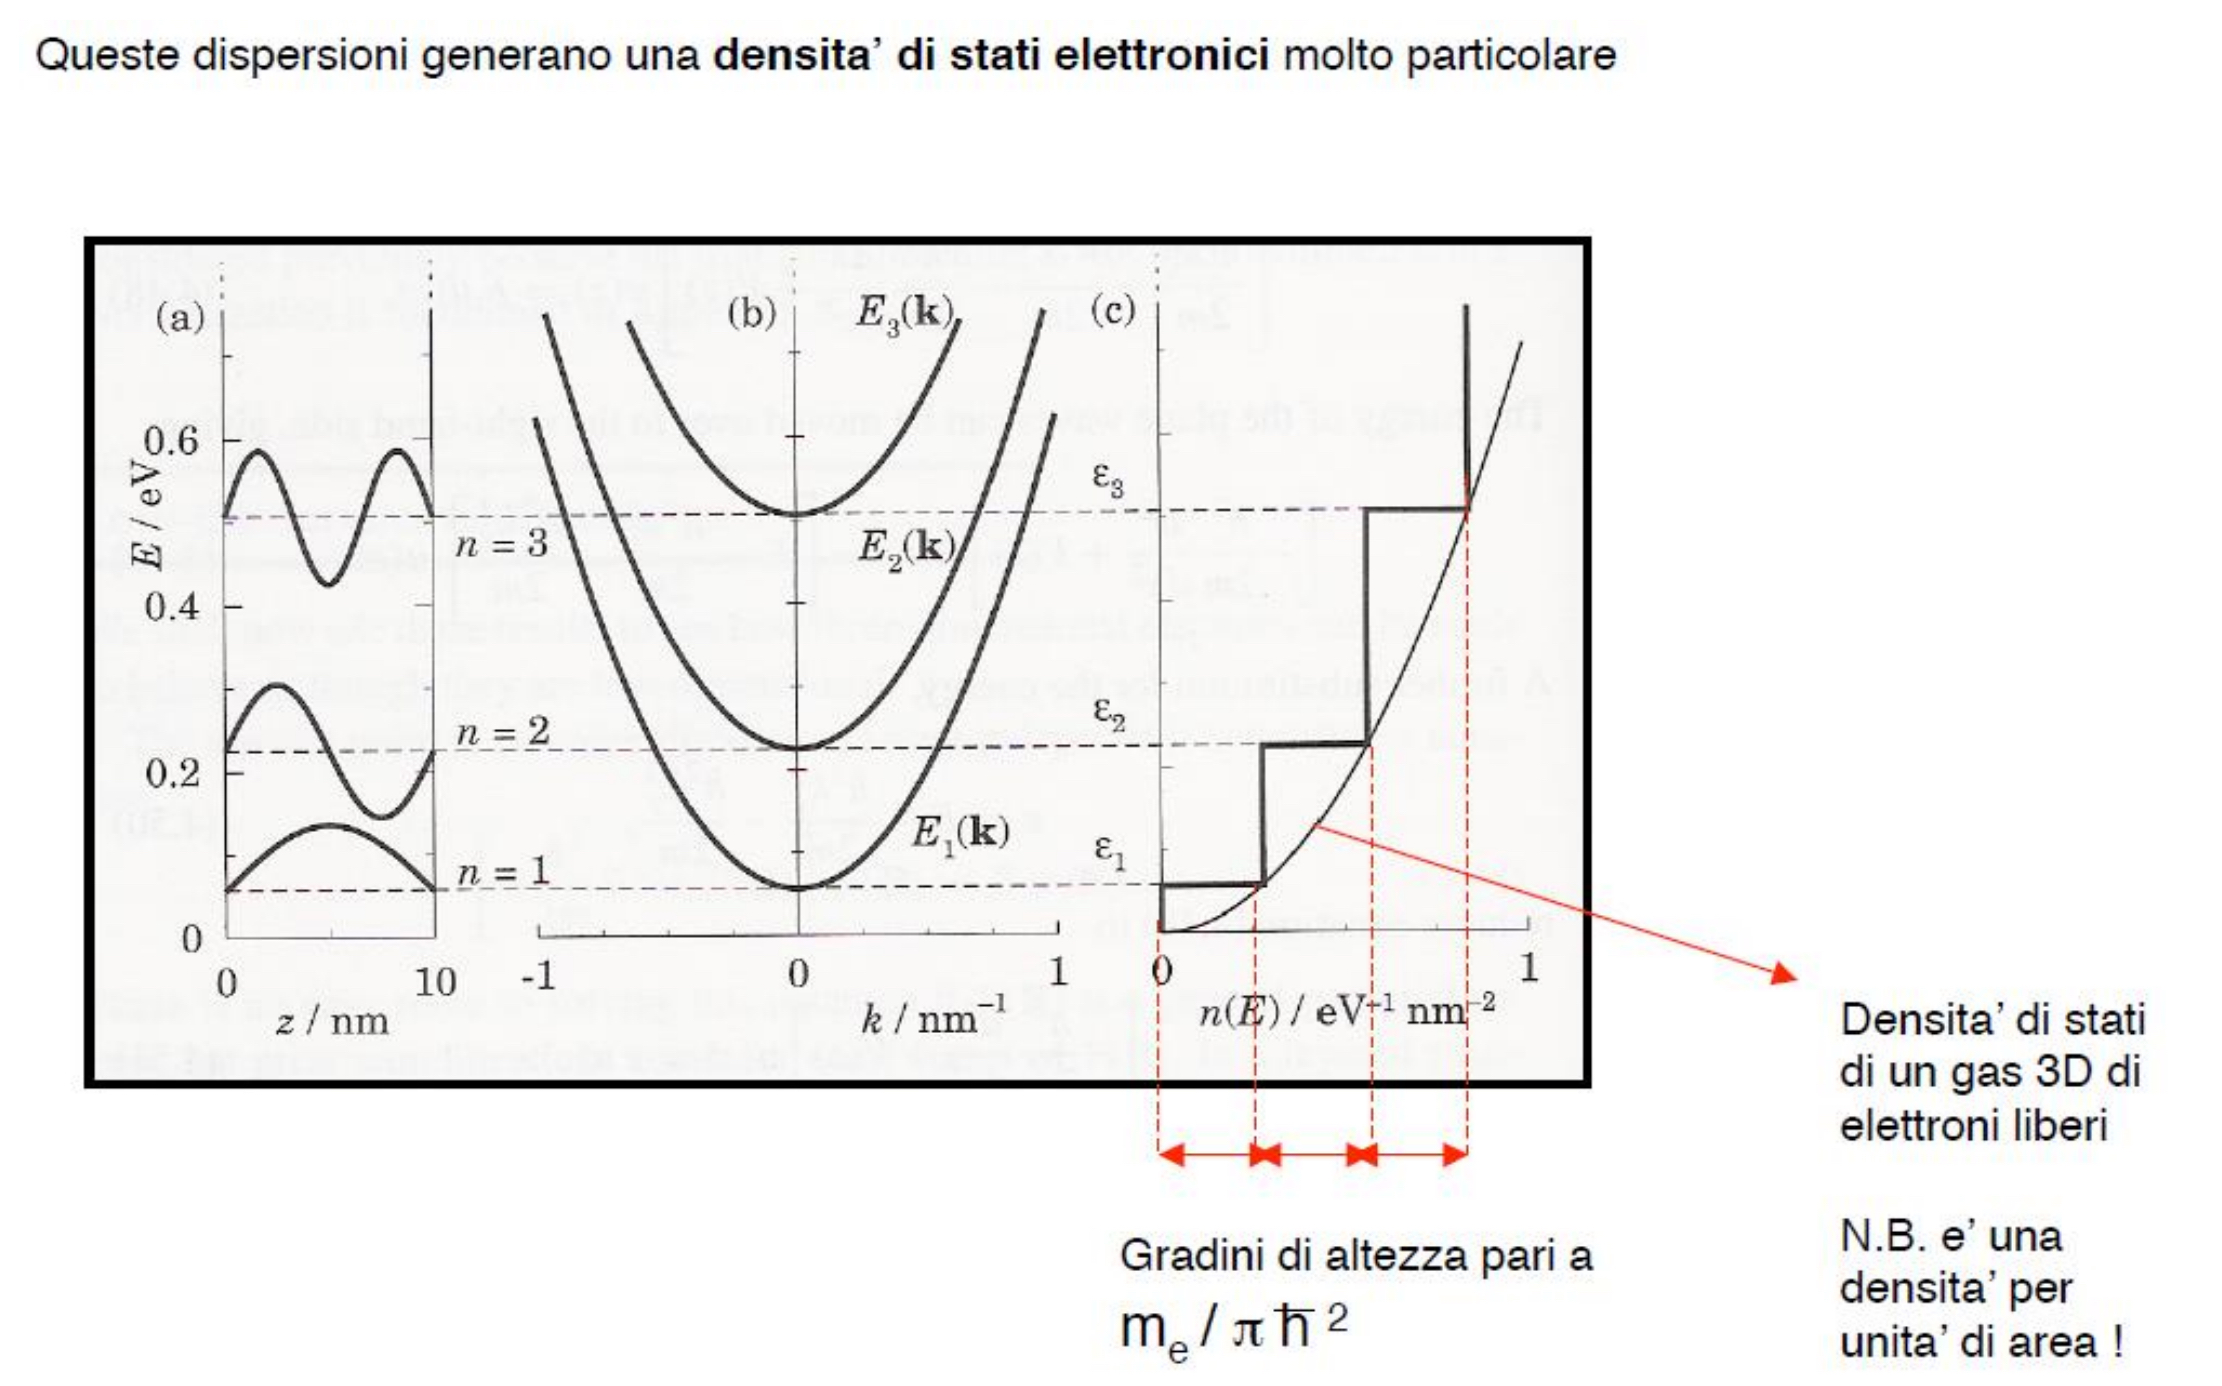
\includegraphics[width=\linewidth]{images/9-Nanostrutture/IMG_1793.jpg}
\caption{Ulteriore rappresentazione grafica del problema.}
\end{figure}
\chapter{Superconduttori}
La superconduttività venne scoperta nel 1911 da Kamerlingh Onnes raffreddando del mercurio tramite l'elio liquido. Si osservò che la conduttività del mercurio aumentava al diminuire della temperatura, quindi la resistenza diminuiva per via della diminuizione degli urti degli elettroni. Però al di sotto di una certa temperatura detta \textbf{temperatura critica} la resistenza R va a zero. Quindi inizialmente si disse che il mercurio era passato ad un nuovo stato nel quale esibiva straordinarie proprieta conduttive chiamato stato superconduttivo.
\section{Effetto Meissner e Variabile di Stato}
Ciò che distingue un semplice conduttore con resistenza molto bassa da un vero superconduttore è la presenza dell'\textbf{effetto Meissner}. Questo fenomeno consiste nell'espulsione totale del campo magnetico dal volume del materiale non appena esso entra nello stato superconduttivo. In altre parole, un superconduttore non permette la penetrazione del campo magnetico interno, indipendentemente dalle condizioni esterne precedenti.
\subsection*{Ragionamento Fisico-Matematico}
Consideriamo il seguente ragionamento: se la resistenza di un materiale tende a zero, allora la conduttività \(\sigma\) tende all'infinito. Dato che la legge di Ohm locale è espressa da
\[
J = \sigma E,
\]
per mantenere una densità di corrente \(J\) finita con \(\sigma \to \infty\) è necessario che il campo elettrico \(E\) sia nullo (altrimenti \(J\) diverrebbe infinito). 
Utilizzando ora la legge di Faraday,
\[
\vec{\nabla} \times E = -\frac{1}{c}\,\frac{\partial B}{\partial t},
\]
se \(E = 0\) allora la sua rotazione è nulla, il che implica che:
\[
\frac{\partial B}{\partial t} = 0.
\]
Questa condizione significa che, se fosse presente un campo magnetico \(B\) all'interno del materiale, esso non cambierebbe nel tempo. Un'analisi superficiale porterebbe dunque a ipotizzare che, al passaggio nello stato superconduttivo, il campo magnetico interno resti costante.
\subsection*{Il Paradosso e l'Effetto Meissner}
Nonostante il ragionamento precedente, le osservazioni sperimentali mostrano che, al calar della temperatura al di sotto di una soglia critica \(T_c\), il materiale espelle il campo magnetico, ottenendo un campo interno nullo (\(B = 0\)). Questo è l'\textbf{effetto Meissner}.\\\\
L'espulsione del campo magnetico fa sì che il campo magnetico non sia una quantità “congelata” (dipendente dalla storia del campione) ma diventi una vera e propria \textbf{variabile di stato}. Ciò significa che lo stato finale di un superconduttore (con \(B = 0\)) è univocamente determinato dalle sue condizioni termodinamiche, indipendentemente dal percorso seguito per raggiungerlo.
\subsection*{Verifica tramite Esperimenti con Sequenze Differenti}
Per mettere in evidenza questo aspetto, consideriamo due procedure sperimentali che portano al medesimo stato finale:
\begin{enumerate}
    \item \textbf{Sequenza con Effetto Meissner:}\\
    In un primo esperimento (vedi Figura \ref{fig:eff}), il materiale viene inizialmente tenuto nello stato normale (temperatura \(T > T_c\)) in presenza di un campo magnetico \(B \neq 0\). Successivamente, raffreddando il materiale al di sotto della temperatura critica, si osserva che il campo magnetico viene espulso, ottenendo infine uno stato superconduttivo in cui \(B = 0\).

    \item \textbf{Sequenza con Raffreddamento Diretto:}\\
    In un secondo esperimento (vedi Figura \ref{fig:eff} a sinistra), il materiale viene prima raffreddato direttamente a \(T < T_c\) e, solo a valle, viene applicato un campo magnetico. In questo caso, il campo non riesce a penetrare nel materiale già superconduttivo, e si ottiene nuovamente un superconduttore con \(B = 0\).
\end{enumerate}
Questi due itinerari portano sempre allo stesso stato finale, dimostrando che il campo magnetico all'interno del superconduttore è una variabile di stato. \\
Al contrario, in assenza dell'effetto Meissner (vedi Figura \ref{fig:noeff}), se il campo magnetico fosse "congelato" nello stato in cui il materiale entra nel regime superconduttivo, la storia del campione determinerebbe lo stato interno. Ad esempio:
\begin{itemize}
    \item Nel primo caso, il materiale, raffreddato in presenza di \(B\), mantenendolo costante a causa di \(\frac{\partial B}{\partial t}=0\), presenterebbe un campo magnetico interno non nullo.
    \item Nel secondo caso, il materiale raffreddato in assenza di campo resterebbe con \(B = 0\).
\end{itemize}
Le due situazioni darebbero così esiti differenti, contraddicendo il concetto di variabile di stato. 

\begin{figure} [H]
    \centering
    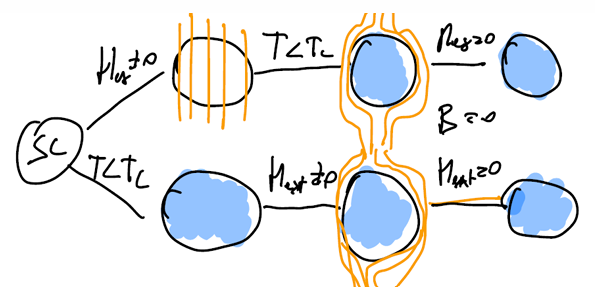
\includegraphics[width=0.7\linewidth]{images/10-Superconduttori/eff meissner.png}
    \caption{}
    \label{fig:eff}
\end{figure}
\begin{figure} [H]
    \centering
    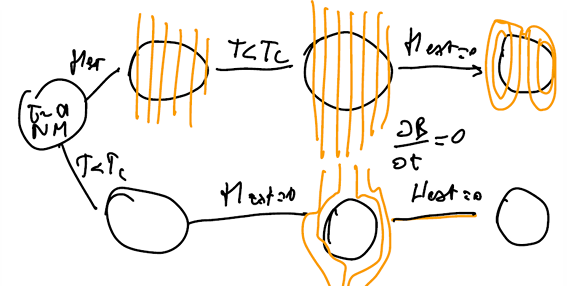
\includegraphics[width=0.7\linewidth]{images/10-Superconduttori/no eff meissner.png}
    \caption{}
    \label{fig:noeff}
\end{figure} 

\section{Origine del Passaggio di Stato e Effetto Meissner}

Il passaggio di stato che porta un materiale a diventare superconduttore non è accompagnato da alcuna modifica della struttura cristallina. Infatti, se si irragge il campione con raggi-X si osserva che la disposizione degli atomi non cambia, e non si registrano transizioni che coinvolgono l'ordine magnetico (ad es. transizioni ferromagnetiche o antiferromagnetiche). \textbf{La transizione è invece dovuta a un cambiamento nello stato elettronico: al passaggio alla fase superconduttiva si apre un gap nell'energia dei livelli elettronici in prossimità del livello di Fermi. Tale apertura comporta una modifica della densità degli stati disponibili e, conseguentemente, delle quantità termodinamiche come l'energia libera e il calore specifico.}

\subsection*{Effetti sul Calore Specifico e sull'Energia Libera}

Osservando l'andamento del calore specifico \(C_V\) e dell'energia libera \(F\) (vedi Figura \ref{fig:calspF}), si evidenzia come la presenza del gap influisca notevolmente sulle proprietà termodinamiche:
\begin{itemize}
    \item \textbf{Calore Specifico:} Nel metallo normale la distribuzione degli stati elettronici attorno al livello di Fermi è continua. Con l'apertura del gap, il numero di stati a disposizione in prossimità di \(E_F\) diminuisce, modificando il contributo entropico del sistema. Questo si traduce in un andamento del calore specifico che differisce sensibilmente da quello del metallo normale.
    \item \textbf{Energia Libera:} La variazione dell'energia libera tra lo stato normale (\(F_N\)) e quello superconduttivo (\(F_S\)) è legata all'energia necessaria per espellere il campo magnetico dal materiale, secondo il rapporto:
    \[
    F_N(T) - F_S(T) = \frac{H_C(T)^2}{8\pi}.
    \]
    Tale termine rappresenta l'energia di espulsione del campo magnetico e risulta strettamente connesso alla variazione dell'entropia tra i due stati.

    \begin{figure}[H]
        \centering
        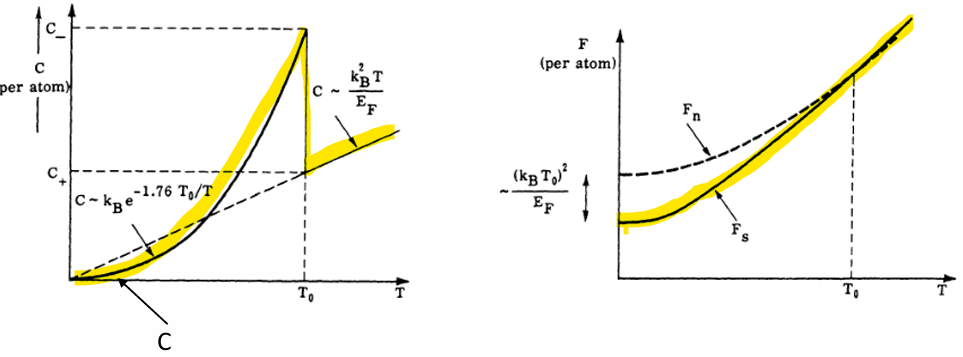
\includegraphics[width=0.9\linewidth]{images/10-Superconduttori/calspF.png}
        \caption{La linea tratteggiata rappresenta l'andamento termodinamico del metallo normale, mentre quella continua evidenzia l'andamento del superconduttore.}
        \label{fig:calspF}
    \end{figure}
\end{itemize}

\subsection*{Superconduttori di Tipo I}
I superconduttori si distinguono in due classi in base alla loro risposta al campo magnetico: \textbf{Tipo I} e \textbf{Tipo II}. Nei superconduttori di Tipo I il campo magnetico viene completamente espulso (effetto Meissner). \\
Considerando il campo magnetico applicato \(H\) come variabile di stato, si può ricavare un diagramma di fase in funzione della temperatura (vedi Figura \ref{fig:diagfaseH1}):
\begin{figure}[H]
    \centering
    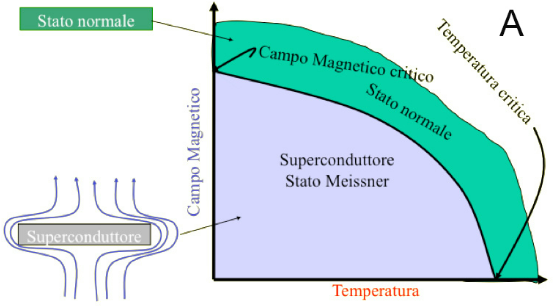
\includegraphics[width=0.7\linewidth]{images/10-Superconduttori/diagfaseH.png}
    \caption{Diagramma di fase per un superconduttore di Tipo I.}
    \label{fig:diagfaseH1}
\end{figure}

Dal diagramma risulta che:
\begin{itemize}
    \item Quando \(H > H_c(T)\) il materiale resta nello stato normale.
    \item Quando \(H < H_c(T)\) il materiale entra nello stato superconduttivo, espellendo il campo magnetico mediante la generazione di correnti di schermo sulla superficie.
\end{itemize}

Il fatto che il superconduttore impieghi una certa quantità di energia per espellere il campo magnetico è correlato alle variazioni entropiche. Per analizzare questo punto si consideri l'energia libera di Helmholtz. Al punto di transizione, quando lo stato normale e quello superconduttivo coesistono, si ha:
\[
F_N(T) = F_S(T) + \frac{H_C(T)^2}{8\pi},
\]
da cui
\[
F_N(T) - F_S(T) = \frac{H_C(T)^2}{8\pi}.
\]
Derivando questa relazione rispetto a \(T\), si ottiene:
\[
\frac{d}{dT}\Bigl[ F_N(T)-F_S(T) \Bigr] = \frac{H_C(T)}{4\pi}\frac{dH_C(T)}{dT}.
\]
Ricordando che l'entropia \(S\) è definita da \(S = -\frac{\partial F}{\partial T}\), segue:
\[
S_S - S_N = \frac{H_C(T)}{4\pi}\frac{dH_C(T)}{dT}.
\]
Dal diagramma di fase, si osserva che \(\frac{dH_C(T)}{dT} < 0\). Quindi:
\[
S_S < S_N,
\]
ovvero la transizione al regime superconduttivo è accompagnata da una diminuzione dell'entropia.

\subsection*{Espulsione del Campo Magnetico e Gap Elettronico}
\textbf{L'espulsione completa del campo magnetico nei superconduttori di Tipo I si ottiene mediante la formazione di correnti di schermo che scorrono in prossimità della superficie del materiale.} Queste correnti creano un campo magnetico che, per effetto di interferenza, annulla il campo esterno all'interno del superconduttore.\\\\

Un ulteriore aspetto fondamentale riguarda il meccanismo che porta alla formazione del gap a livello dell'energia di Fermi. Si può osservare questo fenomeno tracciando la funzione
\[
f\ln f - (1-f)\ln (1-f),
\]
dove \(f\) è la distribuzione di Fermi-Dirac, in funzione del rapporto \(E/E_F\) (vedi Figura \ref{fig:eef}). Tale funzione risulta fortemente concentrata in prossimità di \(E_F\). \\
\textbf{Per ridurre l'entropia e ottenere così un minor numero di stati accessibili nei dintorni di \(E_F\), il sistema evolve in modo da aprire un gap nell'energia dei livelli elettronici.} La riduzione degli stati disponibili è direttamente responsabile della diminuzione dell'entropia che abbiamo osservato derivando l'energia libera.
\begin{figure}[H]
    \centering
    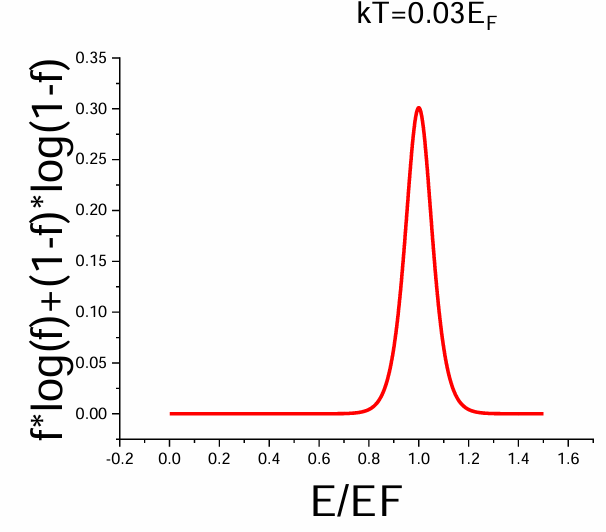
\includegraphics[width=0.7\linewidth]{images/10-Superconduttori/eef.png}
    \caption{Comportamento della funzione \(f\ln f - (1-f)\ln (1-f)\) in funzione di \(E/E_F\). La forte concentrazione in prossimità di \(E_F\) evidenzia come un gap riduca il contributo entropico degli elettroni.}
    \label{fig:eef}
\end{figure}

\subsection*{Calcolo del Calore Specifico al Punto di Transizione}
Per esaminare il punto di transizione, si studia il salto nel calore specifico, che è direttamente collegato alla variazione dell'entropia. Partiamo dalla relazione:
\[
\Delta S = \frac{H_C(T)}{4\pi} \frac{dH_C(T)}{dT}.
\]
Il calore specifico a volume costante in prossimità della temperatura critica \(T_C\) è definito come:
\[
c_V(T_C) = T_C \left( \frac{\partial S}{\partial T} \right)_V.
\]
Calcolando la derivata dell'entropia rispetto a \(T\) si ottiene:
\[
c_V(T_C) = \frac{T_C}{4\pi} \left[ \left( \frac{dH_C}{dT} \right)^2 + H_C(T_C) \left( \frac{d^2 H_C}{dT^2} \right) \right].
\]
Poiché per definizione \(H_C(T_C)=0\) (al punto di transizione il campo critico si annulla), il termine contenente la derivata seconda scompare e si ha:
\[
c_V(T_C) = \frac{T_C}{4\pi} \left( \frac{dH_C}{dT} \right)^2.
\]
Questa espressione evidenzia che il salto del calore specifico in corrispondenza della temperatura critica è determinato esclusivamente dalla pendenza del campo critico in funzione della temperatura.


\subsection{Coppie di Cooper}
L'osservazione sperimentale che la temperatura critica \(T_C\) dipende dall'isotopo, con una relazione del tipo
\[
T_C \sim \frac{1}{\sqrt{M}},
\]
dove \(M\) è la massa ionica, suggerisce fortemente il coinvolgimento dei fononi nel meccanismo di superconduttività. Infatti, sappiamo che la frequenza caratteristica dei fononi (frequenza di Debye) è data da
\[
\omega_D = \sqrt{\frac{K}{M}},
\]
con \(K\) una costante elastica. \\
Ciò implica che all'aumentare della massa ionica la frequenza dei fononi diminuisce, abbassando così \(T_C\). L'interpretazione è che l'interazione mediata dai fononi tra elettroni sia responsabile del legame che forma le cosiddette \textbf{coppie di Cooper}.\\\\

A temperature molto basse, gli elettroni in un metallo possono interagire indirettamente attraverso la deformazione del reticolo cristallino secondo il seguente meccanismo:
\begin{enumerate}
    \item Un elettrone con momento \(\mathbf{k}\) si muove all'interno del reticolo, causando una deformazione locale della rete ionica (essendo gli ioni positivamente carichi).
    \item Questa deformazione genera un'oscillazione del reticolo, che può essere interpretata come l'emissione di un \emph{fonone}.
    \item Un secondo elettrone, avente in qualche modo un momento opposto \(-\mathbf{k}\), viene attratto dalla regione in cui il reticolo è stato deformato, instaurando così un'interazione attrattiva tra i due elettroni. 
\end{enumerate}
Questo meccanismo è alla base della \textbf{BCS theory} (Bardeen-Cooper-Schrieffer), secondo la quale la trasformata di Fourier del potenziale d'interazione tra due elettroni può essere espressa come:
\[
V_S(q,\omega) = \frac{V_q}{\varepsilon(q,\omega)} + \frac{2\omega_D\, M_q^2}{\varepsilon(q,\omega) \left[\omega^2 - \omega_D^2\right]}.
\]
Il primo termine è associato alla repulsione coulombiana intrinseca tra elettroni, mentre il secondo termine, per \(\omega < \omega_D\), può assumere valori negativi (cioè attrattivi) grazie alla mediazione dei fononi. \\
Questa attrazione, se abbastanza intensa, consente a due elettroni di legarsi formando una coppia di Cooper. \\
Le coppie di Cooper si comportano come bosoni e possono condensare in un unico stato quantico macroscopico. Tale condensazione comporta una diminuzione dell'energia del sistema e apre un gap (interruzione) nella densità degli stati elettronici attorno al livello di Fermi:
\[
\Delta = -2\,\hbar\omega_D\, e^{-\frac{2}{N(0)V}},
\]
dove \(V\) è il potenziale attrattivo mediato dai fononi e \(N(0)\) è la densità degli stati alla energia di Fermi. \\
Se l'energia termica \(k_B T\) è inferiore al gap \(\Delta\), le coppie di Cooper non si rompono, mantenendo stabile lo stato superconduttivo e portando a resistenza nulla, poiché le coppie non subiscono scattering.
\section{Superconduttori di Tipo II}

I superconduttori di \textbf{Tipo II}, a differenza di quelli di tipo I, ammettono una penetrazione parziale del campo attraverso la formazione di strutture chiamate \emph{vortici} o \emph{fili quantizzati}, generando così una fase mista.\\
In particolare, il comportamento di un superconduttore di Tipo II al variare del campo magnetico esterno \(H_{\rm ext}\) può essere descritto in tre regimi:
\begin{enumerate}
    \item \(\mathbf{H_{\rm ext} > H_2^{(c)}}\): il materiale si trova nello stato normale; il campo magnetico penetra completamente.
    \item \(\mathbf{H_1^{(c)} < H_{\rm ext} < H_2^{(c)}}\): il materiale mostra una \emph{fase mista} in cui parte del campo magnetico penetra sotto forma di vortici, mentre il resto del materiale rimane superconduttivo.
    \item \(\mathbf{H_{\rm ext} < H_1^{(c)}}\): l'effetto Meissner è completo, e il campo magnetico viene escluso dall'intero campione.
\end{enumerate}
Gran parte dei metalli puri tendono ad essere superconduttori di Tipo I, mentre i composti e le leghe mostrano frequentemente un comportamento di Tipo II. La possibilità di sopportare campi magnetici esterni maggiori e di avere temperature critiche più elevate rende i superconduttori di Tipo II particolarmente utili per applicazioni tecnologiche, quali ad esempio le bobine per i magneti superconduttori.

\subsection{Flusso Quantizzato}
Un aspetto fondamentale della superconduttività è la quantizzazione del flusso magnetico. La descrizione microscopica si basa sul fatto che lo stato superconduttivo è caratterizzato da una funzione d'onda macroscopica \(\psi(r) = |\psi(r)| e^{i\phi(r)}\), dove \(\phi(r)\) è la fase. La densità di corrente superconduttiva è data dall'espressione:
\[
J_s = \frac{e^*}{m^*} |\psi(r)|^2 \left[ \hbar\, \nabla\phi(r) - \frac{e^*}{c}\, \mathbf{A}(r) \right],
\]
dove \(e^* = -2e\) e \(m^*\) sono, rispettivamente, la carica e la massa efficace delle coppie di Cooper, e \(\mathbf{A}(r)\) è il potenziale vettore.\\\\
Consideriamo ora un percorso chiuso che circonda una regione in cui il campo magnetico è confinate (ad esempio, l'interno di un vortice). In un circuito chiuso la funzione d'onda deve essere univoca, dunque la fase deve cambiare di un multiplo intero di \(2\pi\):
\[
\oint \nabla\phi(r) \cdot d\mathbf{l} = 2\pi n,\quad n\in\mathbb{Z}.
\]
Se il campione è in uno stato stazionario (quindi \(J_s = 0\) lungo il percorso chiuso), dall'equazione per \(J_s\) risulta:
\[
\hbar\, \nabla\phi(r) = \frac{e^*}{c}\, \mathbf{A}(r).
\]
Integrando lungo un percorso chiuso \(C\) otteniamo:
\[
\oint_C \nabla\phi(r) \cdot \d\mathbf{l} = \frac{e^*}{\hbar c} \oint_C \mathbf{A}(r) \cdot \d\mathbf{l}.
\]
Utilizzando il teorema di Stokes per il lato destro, si ha:
\[
\oint_C \mathbf{A}(r) \cdot \d\mathbf{l} = \int_S (\vec{\nabla} \times \mathbf{A}(r)) \cdot \d\mathbf{S} = \int_S \mathbf{B} \cdot \d\mathbf{S} = \Phi,
\]
dove \(\Phi\) è il flusso magnetico attraverso la superficie \(S\) racchiusa dal percorso \(C\).\\
Sostituendo si ottiene:
\[
2\pi n = \frac{e^*}{\hbar c}\, \Phi \quad \Longrightarrow \quad \Phi = \frac{2\pi \hbar c}{|e^*|}\, n.
\]
Notando che \(e^* = 2e\) (in modulo) si ha:
\[
\Phi = \frac{h c}{2e}\, n \equiv \Phi_0\, n,
\]
dove \(\Phi_0 = \frac{hc}{2e}\) è il \emph{quanto di flusso magnetico}. Questo risultato dimostra che il flusso magnetico attraverso un vortice in un superconduttore è quantizzato in multipli interi di \(\Phi_0\).


\subsection{Equazione di London}
In un superconduttore (in particolare di Tipo II) il comportamento del campo magnetico e della corrente superconduttiva si descrive attraverso le equazioni di Maxwell locali:
\begin{equation}
    \begin{cases}
        \vec{\nabla} \times \vec{B} = \dfrac{4\pi}{c}\,\vec{J}_s + \dfrac{1}{c}\,\dfrac{\partial\vec{E}}{\partial t},\\[1mm]
        \vec{\nabla} \times \vec{E} = - \dfrac{1}{c}\,\dfrac{\partial \vec{B}}{\partial t}.
    \end{cases}
    \label{eqn:maxwell}
\end{equation}
Qui \(\vec{J}_s\) indica la densità di corrente dei superportatori. Nel contesto della superconduttività si assume che la corrente che scherma il campo magnetico esterno sia data da
\[
\vec{J}_s = - n_s e^* \vec{v}_s,
\]
con \(n_s\) la densità di superportatori, \(e^*\) la carica efficace (per le coppie di Cooper \(e^* = -2e\)) e \(\vec{v}_s\) la loro velocità.\\
Se consideriamo il moto dei superportatori, la loro accelerazione è data dalla legge:
\[
\vec{a} = \frac{d\vec{v}_s}{dt} = - \frac{e^*}{m} \vec{E},
\]
da cui si ricava, derivando la definizione di corrente:
\[
\frac{d\vec{J}_s}{dt} = \frac{n_s (e^*)^2}{m}\, \vec{E}.
\]
Per approfondire il legame tra la corrente e il campo, prendiamo il rotore della corrente. Applicando il rotore all'equazione appena trovata e usando la legge di Faraday:
\[
\vec{\nabla} \times \vec{E} = -\frac{1}{c}\,\frac{\partial \vec{B}}{\partial t},
\]
si ha:
\[
\frac{d}{dt} \Bigl(\vec{\nabla} \times \vec{J}_s\Bigr) = \frac{n_s (e^*)^2}{m} \biggl(\vec{\nabla} \times \vec{E}\biggr)
= - \frac{n_s (e^*)^2}{m}\,\frac{1}{c}\,\frac{\partial \vec{B}}{\partial t}.
\]
Integrando nel tempo, si conclude che la quantità
\[
\vec{\nabla} \times \vec{J}_s + \frac{n_s (e^*)^2}{mc}\, \vec{B}
\]
è costante. Impostando opportunamente le condizioni al contorno (ossia, \textbf{scegliendo la costante pari a zero affinché il sistema minimizzi l'energia}), si ottiene la \textbf{Equazione di London}:
\begin{equation}
    \vec{\nabla} \times \vec{J}_s + \frac{n_s (e^*)^2}{mc}\, \vec{B} = 0.
    \label{eqn:london1}
\end{equation}

\subsubsection*{Caso Elettrostatico}
In condizioni elettrostatiche, \(\frac{\partial \vec{E}}{\partial t}=0\), si può riscrivere la relazione di Londono usando la prima equazione di Maxwell (\ref{eqn:maxwell}):
\[
\vec{J}_s = \frac{c}{4\pi}\, \vec{\nabla} \times \vec{B}.
\]
Calcolando il rotore di questa espressione:
\[
\vec{\nabla} \times \vec{J}_s = \frac{c}{4\pi}\, \vec{\nabla} \times (\vec{\nabla} \times \vec{B}).
\]
Usiamo ora l'identità vettoriale
\[
\vec{\nabla} \times (\vec{\nabla} \times \vec{B}) = \nabla(\vec{\nabla} \cdot \vec{B}) - \nabla^2 \vec{B},
\]
ma poiché \(\vec{\nabla} \cdot \vec{B}=0\), la relazione si riduce a:
\[
\vec{\nabla} \times (\vec{\nabla} \times \vec{B}) = -\nabla^2 \vec{B}.
\]
Sostituendo nell'Equazione di London (\ref{eqn:london1}), si ottiene:
\[
\frac{c}{4\pi} \, \bigl(-\nabla^2 \vec{B}\bigr) + \frac{n_s (e^*)^2}{mc}\, \vec{B} = 0,
\]
cioè:
\[
\nabla^2 \vec{B} = \frac{4\pi n_s (e^*)^2}{mc^2}\, \vec{B}.
\]
Definendo la lunghezza di penetrazione (o \textbf{lunghezza di London}) \(\lambda_L\) tramite
\[
\frac{1}{\lambda_L^2} = \frac{4\pi n_s (e^*)^2}{mc^2},
\]
l'equazione diventa:
\begin{equation}
    \nabla^2 \vec{B} = \frac{1}{\lambda_L^2}\, \vec{B}.
    \label{eqn:london2}
\end{equation}
\textbf{Questa equazione indica che il campo magnetico si attenua esponenzialmente all'interno del superconduttore con lunghezza caratteristica \(\lambda_L\).}

\subsection{Derivazione Energetica dell'Equazione di London}
La condizione per cui l'equazione di London assume il lato destro nullo deriva dalla minimizzazione dell'energia totale del sistema. L'energia totale \(E\) in un superconduttore comprende:
\begin{itemize}
    \item L'energia del sistema intrinseco, \( \int F_s \, \d\vec{r} \).
    \item L'energia cinetica \(E_k\) associata al moto dei superportatori.
    \item L'energia magnetica \(E_{mag}\).
\end{itemize}
L'energia cinetica è data da:
\[
E_k = \int \frac{1}{2} m\, n_s\, \vec{v}_s^2 \, \d\vec{r},
\]
mentre, sfruttando la relazione locale:
\[
\vec{v}_s = \frac{\vec{J}_s}{n_s e^*}
\]
e l'equazione di Maxwell in forma locale:
\[
\vec{J}_s = \frac{c}{4\pi}\, (\vec{\nabla} \times \vec{h}),
\]
si può esprimere \(E_k\) in funzione del campo magnetico. Dopo alcune manipolazioni, si giunge ad una forma del tipo:
\[
E_k = \int \frac{1}{8\pi} \lambda_L^2\, (\vec{\nabla} \times \vec{h})^2\, \d\vec{r},
\]
dove \(\vec{h}\) indica il campo magnetico locale.
L'energia magnetica invece è:
\[
E_{mag} = \int \frac{\vec{h}^2}{8\pi}\, \d\vec{r}.
\]
Pertanto, l'energia totale diventa:
\[
E = E_0 + \frac{1}{8\pi}\int \left[\vec{h}^2 + \lambda_L^2\, (\vec{\nabla} \times \vec{h})^2\right] \d\vec{r}.
\]
Minimizzando quest'energia rispetto alle variazioni \(\delta \vec{h}\) (ossia imponendo \(\delta E = 0\)) si ottiene:
\[\delta E = \frac{1}{8\pi} \cdot \int [2\vec{h}+2\cdot \lambda^2_L\cdot\vec{\nabla}\times(\vec{\nabla}\times \vec{h})]\cdot\delta \vec{h}\cdot \d\vec{r} = \frac{1}{4\pi}\cdot \int [\vec{h}-\lambda^2_L\cdot \nabla^2\vec{h}]\cdot\delta \vec{h}\cdot \d\vec{r}= 0\]
Ossia:
\[
\vec{h} - \lambda_L^2 \, \nabla^2 \vec{h} = 0,
\]
la quale è equivalente all'equazione (\ref{eqn:london2}) ricavata in precedenza. Il fatto che l'energia si minimizzi corrisponde fisicamente alla scelta della costante nulla nella relazione
\[
\vec{\nabla} \times \vec{J}_s + \frac{n_s (e^*)^2}{mc}\, \vec{B} = \text{costante}.
\]

\subsection{Esempio: Campo Magnetico Orientato}
Consideriamo ora il caso in cui il campo magnetico ha una specifica direzione e studiamo il comportamento delle correnti superficiali.\\
\paragraph{Caso 1:} \(\vec{h} \parallel \hat{z}\) \\
Se il campo è orientato lungo \(z\) allora, per la condizione \(\vec{\nabla} \cdot \vec{h} = 0\), si ha che le variazioni lungo \(z\) sono nulle e il rotore risulta nullo. Di conseguenza, in questo caso non vi sono correnti, ossia \(\vec{J} = 0\).\\\\

\paragraph{Caso 2:} \(\vec{h} \parallel \hat{x}\) o \(\vec{h} \parallel \hat{y}\) \\
Quando il campo è orientato in una direzione trasversale, l'unica variazione non nulla risiede nella direzione \(z\). In tal caso, considerando che
\[
\vec{\nabla} \times \vec{h} = \frac{4\pi}{c}\, \vec{J},
\]
l'unica componente non nulla del rotore è data da
\[
\frac{\partial h}{\partial z} = \frac{4\pi}{c}\, J.
\]
Applicando l'equazione di London (\ref{eqn:london2}) per l'andamento del campo lungo \(z\), si ha:
\[
\frac{\partial^2 h}{\partial z^2} = \frac{1}{\lambda_L^2}\, h,
\]
la cui soluzione è
\[
h(z) = h(0)\, e^{-z/\lambda_L}.
\]
Pertanto, \textbf{le correnti di schermo che schermano il campo magnetico sono localizzate sulla superficie del superconduttore e decrescono esponenzialmente con la profondità \(\lambda_L\).}\\\\
Inoltre, dalla relazione di London è possibile ricavare come varia la densità di corrente con \(z\):
\[ \vec{h} + \lambda_L^2\cdot \vec{\nabla}\times(\vec{\nabla}\times \vec{h})=0\]
 \[ \vec{h} + \lambda_L^2\cdot \vec{\nabla}\times\biggr(\frac{4\pi}{c}\cdot \vec{j}\biggr)=0 \]
        soppravvive solo una componente:
 \[\vec{h} - \frac{mc^2}{4\pi n_s e^2}\cdot \frac{4\pi}{c}\cdot \frac{\partial \vec{j}}{\partial z} = 0 \implies \frac{\partial \vec{j}}{\partial z} = \frac{n_s e^2}{mc}\cdot \vec{h}\]
\[
\frac{\partial \vec{J}}{\partial z} \propto \vec{h}.
\]

\subsection{Scelta del Gauge e Equazione Locale di London}
Consideriamo l'equazione di London nella forma
\[
\vec{\nabla} \times \vec{J}_s + \frac{n_s (e^*)^2}{mc}\, \vec{B} = 0,
\]
con 
\[
\vec{B} = \vec{\nabla} \times \vec{A},
\]
Per semplificare il problema, scegliamo il \emph{gauge di London}, il quale impone:
\[
\vec{\nabla} \cdot \vec{A} = 0.
\]
Questa condizione implica che:
\[
\nabla^2\phi = - \vec{\nabla} \cdot \vec{A} = 0,
\]
 Per semplicità si può imporre
\[
\phi = \text{costante} = 0,
\]
Inoltre, imponiamo la condizione di assenza di sorgenti per la corrente superconduttiva:
\[
\vec{\nabla} \cdot \vec{J}_s = 0.
\]
Sotto queste condizioni, l'equazione di London si riscrive, sostituendo \(\vec{B} = \vec{\nabla} \times \vec{A}\), come:
\[
\vec{\nabla} \times \vec{J}_s + \frac{n_s (e^*)^2}{mc}\, (\vec{\nabla} \times \vec{A}) = 0.
\]
Poiché il rotore è un operatore lineare, possiamo scrivere una relazione locale puntuale separando i due termini. In particolare, scegliendo opportunamente le condizioni al contorno affinché la costante di integrazione sia zero (equivalente a minimizzare l'energia del sistema) si ottiene:
\[
\vec{\nabla} \times \vec{J}_s = -\frac{n_s (e^*)^2}{mc}\, (\vec{\nabla} \times \vec{A}).
\]
Integrando, si giunge alla relazione locale:
\[
\vec{J}_s = -\frac{n_s (e^*)^2}{mc}\, \vec{A}.
\]
Questa espressione esprime una dipendenza puntuale della corrente dal potenziale vettore ed è valida quando la risposta del superconduttore al campo magnetico è "istantanea" o locale.

\subsection{Validità della Relazione Locale: Ruolo della Lunghezza di Correlazione \protect{$\zeta_0$}}
Il fatto di avere una relazione locale, come quella appena ottenuta, richiede che il materiale risponda "rapidamente" alla variazione del potenziale vettore. Fisicamente ciò significa che le coppie di Cooper devono essere rigidamente vincolate e la loro coerenza locale deve essere elevata. Tale rigidità è caratterizzata da una lunghezza di correlazione \(\zeta_0\) (detta anche lunghezza di coerenza).\\\\
Si verificano due casi:
\begin{enumerate}
    \item \textbf{Se \(\zeta_0 \gg \lambda_L\):}  
    La lunghezza di correlazione è molto maggiore rispetto alla lunghezza di penetrazione di London \(\lambda_L\). In questo caso, la risposta del materiale al campo magnetico non è effettivamente locale, ovvero il potenziale vettore varia significativamente nell'intorno spaziale definito da \(\zeta_0\). La relazione locale \(\vec{J}_s \propto \vec{A}\) perde di consistenza e bisogna adottare una descrizione non locale; questo è tipico dei superconduttori del tipo Pippard, che vengono solitamente classificati come superconduttori di Tipo I.
    
    \item \textbf{Se \(\zeta_0 \ll \lambda_L\):}  
    La lunghezza di coerenza è molto piccola rispetto a quella di London, e quindi il potenziale vettore si può considerare praticamente costante su scala \(\zeta_0\). In questo caso, la relazione locale \(\vec{J}_s = -\frac{n_s (e^*)^2}{mc}\, \vec{A}\) è valida; si tratta del comportamento tipico dei superconduttori di London, che rientrano nella categoria dei superconduttori di Tipo II.

\end{enumerate}

\subsection{Stima della Lunghezza di Correlazione \(\zeta_0\)}
Per stimare \(\zeta_0\) si utilizza una considerazione basata sul principio di indeterminazione.\\\\
Quando, a \(T = T_c\), si apre un gap \(\Delta\) nella densità degli stati \(g(E)\), gli elettroni in prossimità della Fermi–energy si accoppiano e formano le coppie di Cooper. Queste coppie sono caratterizzate da un certo "pacchetto d'onda" che ha una dimensione spaziale. Dal principio di indeterminazione vale:
\[
\delta p\, \delta x \approx \hbar.
\]
Prendiamo \(\delta x\) come la lunghezza di correlazione \(\zeta_0\). La variazione di impulso \(\delta p\) può essere stimata considerando che gli elettroni coinvolti variano nella loro energia attorno a \(\varepsilon_F\) in un intervallo di ordine \(\Delta\). Pertanto, se consideriamo:
\[
\frac{(p_F+\delta p)^2}{2m} \approx \varepsilon_F + \Delta,
\]
espandendo per piccoli \(\delta p\) si ha:
\[
\frac{p_F^2}{2m} + \frac{p_F\,\delta p}{m} \approx \varepsilon_F + \Delta.
\]
Poiché \(\frac{p_F^2}{2m} = \varepsilon_F\), si ottiene:
\[
\frac{p_F\,\delta p}{m} \approx \Delta \quad \implies \quad \delta p \approx \frac{m\Delta}{p_F}.
\]
Utilizzando la definizione della velocità di Fermi \(v_F = \frac{p_F}{m}\), risulta:
\[
\delta p \approx \frac{\Delta}{v_F}.
\]
Pertanto, dal principio di indeterminazione:
\[
\zeta_0 \approx \delta x \approx \frac{\hbar}{\delta p} \approx \frac{\hbar v_F}{\Delta}.
\]
Spesso per una definizione più precisa si introduce una costante di proporzionalità (ad esempio \(\pi\)), ottenendo:
\[
\zeta_0 \approx \frac{\hbar v_F}{\pi \Delta}.
\]
Quindi, la lunghezza di correlazione \(\zeta_0\) dipende dalla velocità di Fermi e dal gap \(\Delta\).

\subsection{Pippard Kernel}
Nel caso in cui il superconduttore non risponda in modo locale (\(\zeta_0 \gg \lambda_L\)), la relazione tra la densità di corrente e il potenziale vettore non può essere espressa in modo puntuale. In altre parole, la corrente in un punto \(\vec{r}\) dipende non solo da \(\vec{A}(\vec{r})\) ma anche dai valori del potenziale vettore in un intorno della dimensione dell'ordine di \(\zeta_0\). \\
Tale comportamento non locale viene introdotto mediante una relazione fenomenologica, detta \textbf{Pippard Kernel}, che è espressa come:
\[
\vec{j}(\vec{r}) = C \int \frac{\bigl[\vec{A}(\vec{r}') \cdot \vec{R}\bigr]\, \vec{R}}{R^4}\, e^{-R/\zeta_0}\ \d\vec{r}',\quad \text{con } \vec{R} = \vec{r} - \vec{r}',
\]
dove \(C\) è una costante che si determina in base al sistema e alle condizioni di bordo.\\\\
In pratica, se \(\vec{A}\) varia molto lentamente su lunghezze dell'ordine di \(\zeta_0\) (ossia, se \(\vec{A}\) è quasi costante all'interno del volume caratterizzato da \(\zeta_0\)), il kernel si riduce ad una forma che connette le lunghezze caratteristiche. \\
In particolare, si può dimostrare che:
\[
\lambda^3 = \lambda_L^2\, \zeta_0,
\]
e la soluzione per il campo magnetico che penetra nel superconduttore assume la forma:
\[
h(z) = h(0)\, e^{-z/\lambda},
\]
dove \(\lambda\) è la lunghezza di penetrazione effettiva in presenza del comportamento non locale.\\\\
Quindi, in un superconduttore di tipo 1 (dove \(\zeta_0 \gg \lambda_L\)) la non località mette in relazione la lunghezza d'onda del sistema (\(\lambda\)) con la lunghezza di correlazione \(\zeta_0\) e la profondità di penetrazione di London \(\lambda_L\). In questo caso la risposta del sistema al campo magnetico non può essere considerata come una funzione puntuale, ma si deve tenere conto dell'influenza del potenziale vettore in un intorno spaziale dato da \(\zeta_0\).


\subsection{Considerazioni Energetiche}
Dal punto di vista energetico, l'introduzione di un'interfaccia (ad esempio, tra il superconduttore e un metallo normale) comporta una variazione dell'energia superficiale \(\gamma\) (energia per unità di area).  
Il contributo energetico totale di un campione contenente un'interfaccia si scrive:
\[
E = \int \d\vec{r}\,\Bigl(F_n - \frac{H_c^2}{8\pi}\Bigr) + \gamma\, S,
\]
dove \(F_n\) è l'energia libera del metallo normale, \(H_c\) è il campo critico e \(S\) l'area dell'interfaccia.  
Si trovano due casi:
\begin{enumerate}
    \item \textbf{Tipo I} (\(\zeta_0 \gg \lambda_L\)): L'interfaccia aumenta l'energia del sistema (cioè, \(\gamma > 0\)), perturbando il superconduttore. Un'approssimazione è:
    \[
    \gamma \approx \frac{H_c^2}{8\pi}\,\zeta_0.
    \]
    \item \textbf{Tipo II} (\(\zeta_0 \ll \lambda_L\)): Qui l'energia superficiale \(\gamma\) può essere negativa, con un guadagno energetico per il sistema, così che:
    \[
    \gamma \approx - \frac{H_c^2}{8\pi}\,\lambda.
    \]
\end{enumerate}
Infine, se consideriamo l'energia per unità di lunghezza associata ad un vortice (cioè, l'energia in un sistema con flusso quantizzato), si ottiene:
\[
\frac{E}{l} \sim \left(\frac{\Phi_0}{4\pi\lambda}\right)^2 \ln\biggl(\frac{\lambda}{\zeta_0}\biggr),
\]
dove \(\Phi_0 = \frac{hc}{2e}\) è il quanto di flusso magnetico. Questo risultato mostra che, dal punto di vista energetico, conviene far penetrare un singolo vortice (o filamento quantizzato) per volta, piuttosto che più vortici contemporaneamente.




\end{document}